\documentclass{article} % For LaTeX2e

%%% 
% STANDARD PREAMBLE
%%%
%https://tex.stackexchange.com/questions/68821/is-it-possible-to-create-a-latex-preamble-header
\usepackage{/Users/mwojno01/Repos/latex_preamble/preamble}

%%% 
% ACTIVE VS PASSIVE AUDIENCES
%%%

% CREATE DIFFERENT VERSIONS DEPENDING ON THE AUDIENCE
% Reference: https://ramblingacademic.com/2016/10/31/multiple-latex-document-versions/
% Audience choices here: {active, passive}
% The "active" audience is used when teaching and I want to give little exercises. The "passive" version is for study group where we just want to talk through things.

% Define the switch here using "newif" and start its name with "if"
% Here, NAME_OF_SWITCH == "OneCol"
\newif\ifActive

% By default, a switch is "false". Use \NAME_OF_SWITCHtrue to set to true
% Uncomment the line below to set the switch to "true"
%\Activetrue


% USAGE:
%\ifActive 
%% stuff
%\else
%% stuff
%\fi
     
%%% 
% SPECIFIC TO THIS DOCUMENT
%%%

% FASTER LIMITS, INTEGRALS AND SUMS
\newcommand{\dlim}{\ds\lim}
\newcommand{\dint}{\ds\int}
\newcommand{\dsum}{\ds\sum}
\newcommand{\dmu}{\wrt{\mu}}

% SIGMA-FIELDS 
% Sigma fields (text)
\renewcommand{\sf}{$\sigma$-field}
\newcommand{\sfs}{$\sigma$-fields}


% SET FUNCTIONS 
%Finitely additive set functions
\newcommand{\fasf}{\tilde{\mu}_0}
% Signed measure
\newcommand{\signedmu}{\wt{\mu}}

% CARATHEODORY
\newcommand{\Caratheodory}{Carath\'eodory}



% RATIONALS
\renewcommand{\Q}{\mathbb{Q}}


% EPSILON TILDE
\newcommand{\epsilontilde}{\widetilde{\epsilon}}

% MODES OF CONVERGENCE
\newcommand{\convergenceAE}{\stackrel{a.e.}{\to}}
\newcommand{\convergenceAU}{\stackrel{AU}{\to}}
\newcommand{\convergenceInMu}{\stackrel{\mu}{\to}}
\newcommand{\convergenceInLp}{\stackrel{L^p}{\to}}
\newcommand{\convergenceInLinfty}{\stackrel{L^\infty}{\to}}
\newcommand{\weakConvergence}{\stackrel{w}{\to}}


\newcommand{\notConvergenceAE}{\stackrel{a.e.}{\not\to}}
\newcommand{\notConvergenceAU}{\stackrel{AU}{\not\to}}
\newcommand{\notConvergenceInMu}{\stackrel{\mu}{\not\to}}
\newcommand{\notConvergenceInLp}{\stackrel{L^p}{\not\to}}
\newcommand{\notConvergenceInLinfty}{\stackrel{L^\infty}{\not\to}}

% MAKE INTO A CYLINDER
\newcommand{\cylinder}[1]{\widehat{#1}}

% INTERIOR
\newcommand{\interior}[1]{{#1}^\circ}

\begin{document}

\title{Notes on Probability and Measure Theory} 
\maketitle
\setcounter{tocdepth}{2}
\tableofcontents
\newpage 

\section{Overview}

\subsection{References}
These notes are geared towards statisticians, computer scientists, engineers, and others who are interested in measure theory in the service of data science (specifically, statistics or statistical machine learning).  The primary reference is \cite{ash2000probability}.   The book is wonderful for statistical machine learning – it is rigorous,  but also accessible (prerequisites are undergrad-level real analysis and mathematical probability).  Most importantly, it is structured to build towards the kinds of applications in probability that we care about.   (A point of contrast would be a book like that of Stein and Shakarchi, which tends to dwell heavily on things that are of higher interest to pure mathematicians – Cantor sets and fractals, etc.) 

 Unless otherwise specified, all references to the ``text" refers to this textbook.  Likewise the symbol $\S$ refers to a Section of that textbook.
 
 Other useful references are \cite{folland1999real} and \cite{rudin1987real} for filling in depth.  \citet{durrett2010probability} has nice examples and high-level overviews, but in my view does not provide enough detail to become fluent in the topic.
 
\subsection{Motivation for topic} \label{sec:motivation_for_topic}

What are some motivations for measure theory?

\begin{itemize}
\item Measure theory underpins some of the most interesting research in Bayesian statistics and probabilistic machine learning (see work from Stephen G. Walker, Michael Jordan, Tamara Broderick, David Dunson, and so on).   Thus, fluency with measure theory opens doors to a higher level of research consumption. 
\item Measure theory underpins research on stochastic processes (as used in Bayesian nonparametrics) and stochastic differential equations (useful for continuous-time time series models, a current topic of active research interest in machine learning).\footnote{For instance, Gaussian processes do not have densities, and so the common presentation of basic tools (e.g., Bayes theorem, KL divergence) no longer applies.} 
\item Measure theory is convenient in unifying various kinds of random variables.\footnote{For example, it allows one to work with discrete and absolutely continuous random variables in a unified way.  For example, the exponential family includes both types of random variables.}
\item Lebesgue integration provide nice limit theorems, e.g. clarifying when one can interchange integrals and limits (such as derivatives).   
\item Lebesgue integrals can be seen as the completion of Riemann integrals (in the same way that the real numbers complete the rationals).
\item Abstract Lebesgue integration allows one to integrate over spaces more general than the reals. 

\end{itemize}



\subsection{Motivation for notes}

It is hard to beat directly consulting a textbook (such as \cite{ash2000probability}) written by a seasoned mathematician who is an excellent pedagogue. However, we have created these notes nonetheless in an attempt to \textit{support lecture and/or discussion}.   With that goal in mind, we:
\begin{itemize}
\item Format the presentation to encourage easier absorption.\footnote{E.g., we exploit space to organize the presentation, whereas a textbook will often provide proofs in paragraph form. We sometimes refactor presentations into more modular subsections.}
\item Add sketches to support intuition.
\item Curate the text.\footnote{We highlight some of the main themes (and cores of proofs), offloading additional detail to the text.} 
\item Provide additional detail in proofs.  Sometimes alternate paths have been given that seemed ``nicer" to me. 
\item Add remarks (illustrating the need for propositions, the utility of theorems, or connections between things).
\item Incorporate supporting material from outside sources (or worked homework problems).
\item Give some examples and notes for data scientists.\footnote{This is a work in progress.}
\end{itemize}


%We begin with a discussion of $\sigma$-fields, which are the domains of probability measures, and measures more generally.  As it turns out, measures cannot be defined on all subsets of many spaces that we would like to deal with. For instance, consider Proposition 1.2.6 of \cite{rosenthal2006first} which asserts the existence of non-measurable sets for the uniform distribution.  In particular, there is no definition of $P(A)$ that is defined for all subsets $A \subseteq [0,1]$ satisfying all three conditions below



\section{$\S$ 1.1: Some notes on set theory}

\subsection{Limits of sequences of sets}

\begin{definition}
The \textbf{upper limit} of a sequence of sets is given by
\[ \lim\sup A_n := \bigcap_{n=1}^\infty \bigcup_{k \geq n} A_k \]
Alternatively,
\[ x \in \lim\sup A_n \text{ iff } x \in A_n \text{ for infinitely many } n \]
\label{def:upper_limit}
\end{definition}

\begin{definition}
The \textbf{lower limit} of a sequence of sets is given by
\[ \lim\inf A_n := \bigcup_{n=1}^\infty \bigcap_{k \geq n} A_k \]
Alternatively,
\[ x \in \lim\inf A_n \text{ iff } x \in A_n \text{ eventually ( for all but finitely many $n$ ) } \]
\end{definition}

\begin{figure}[H]
\centering 
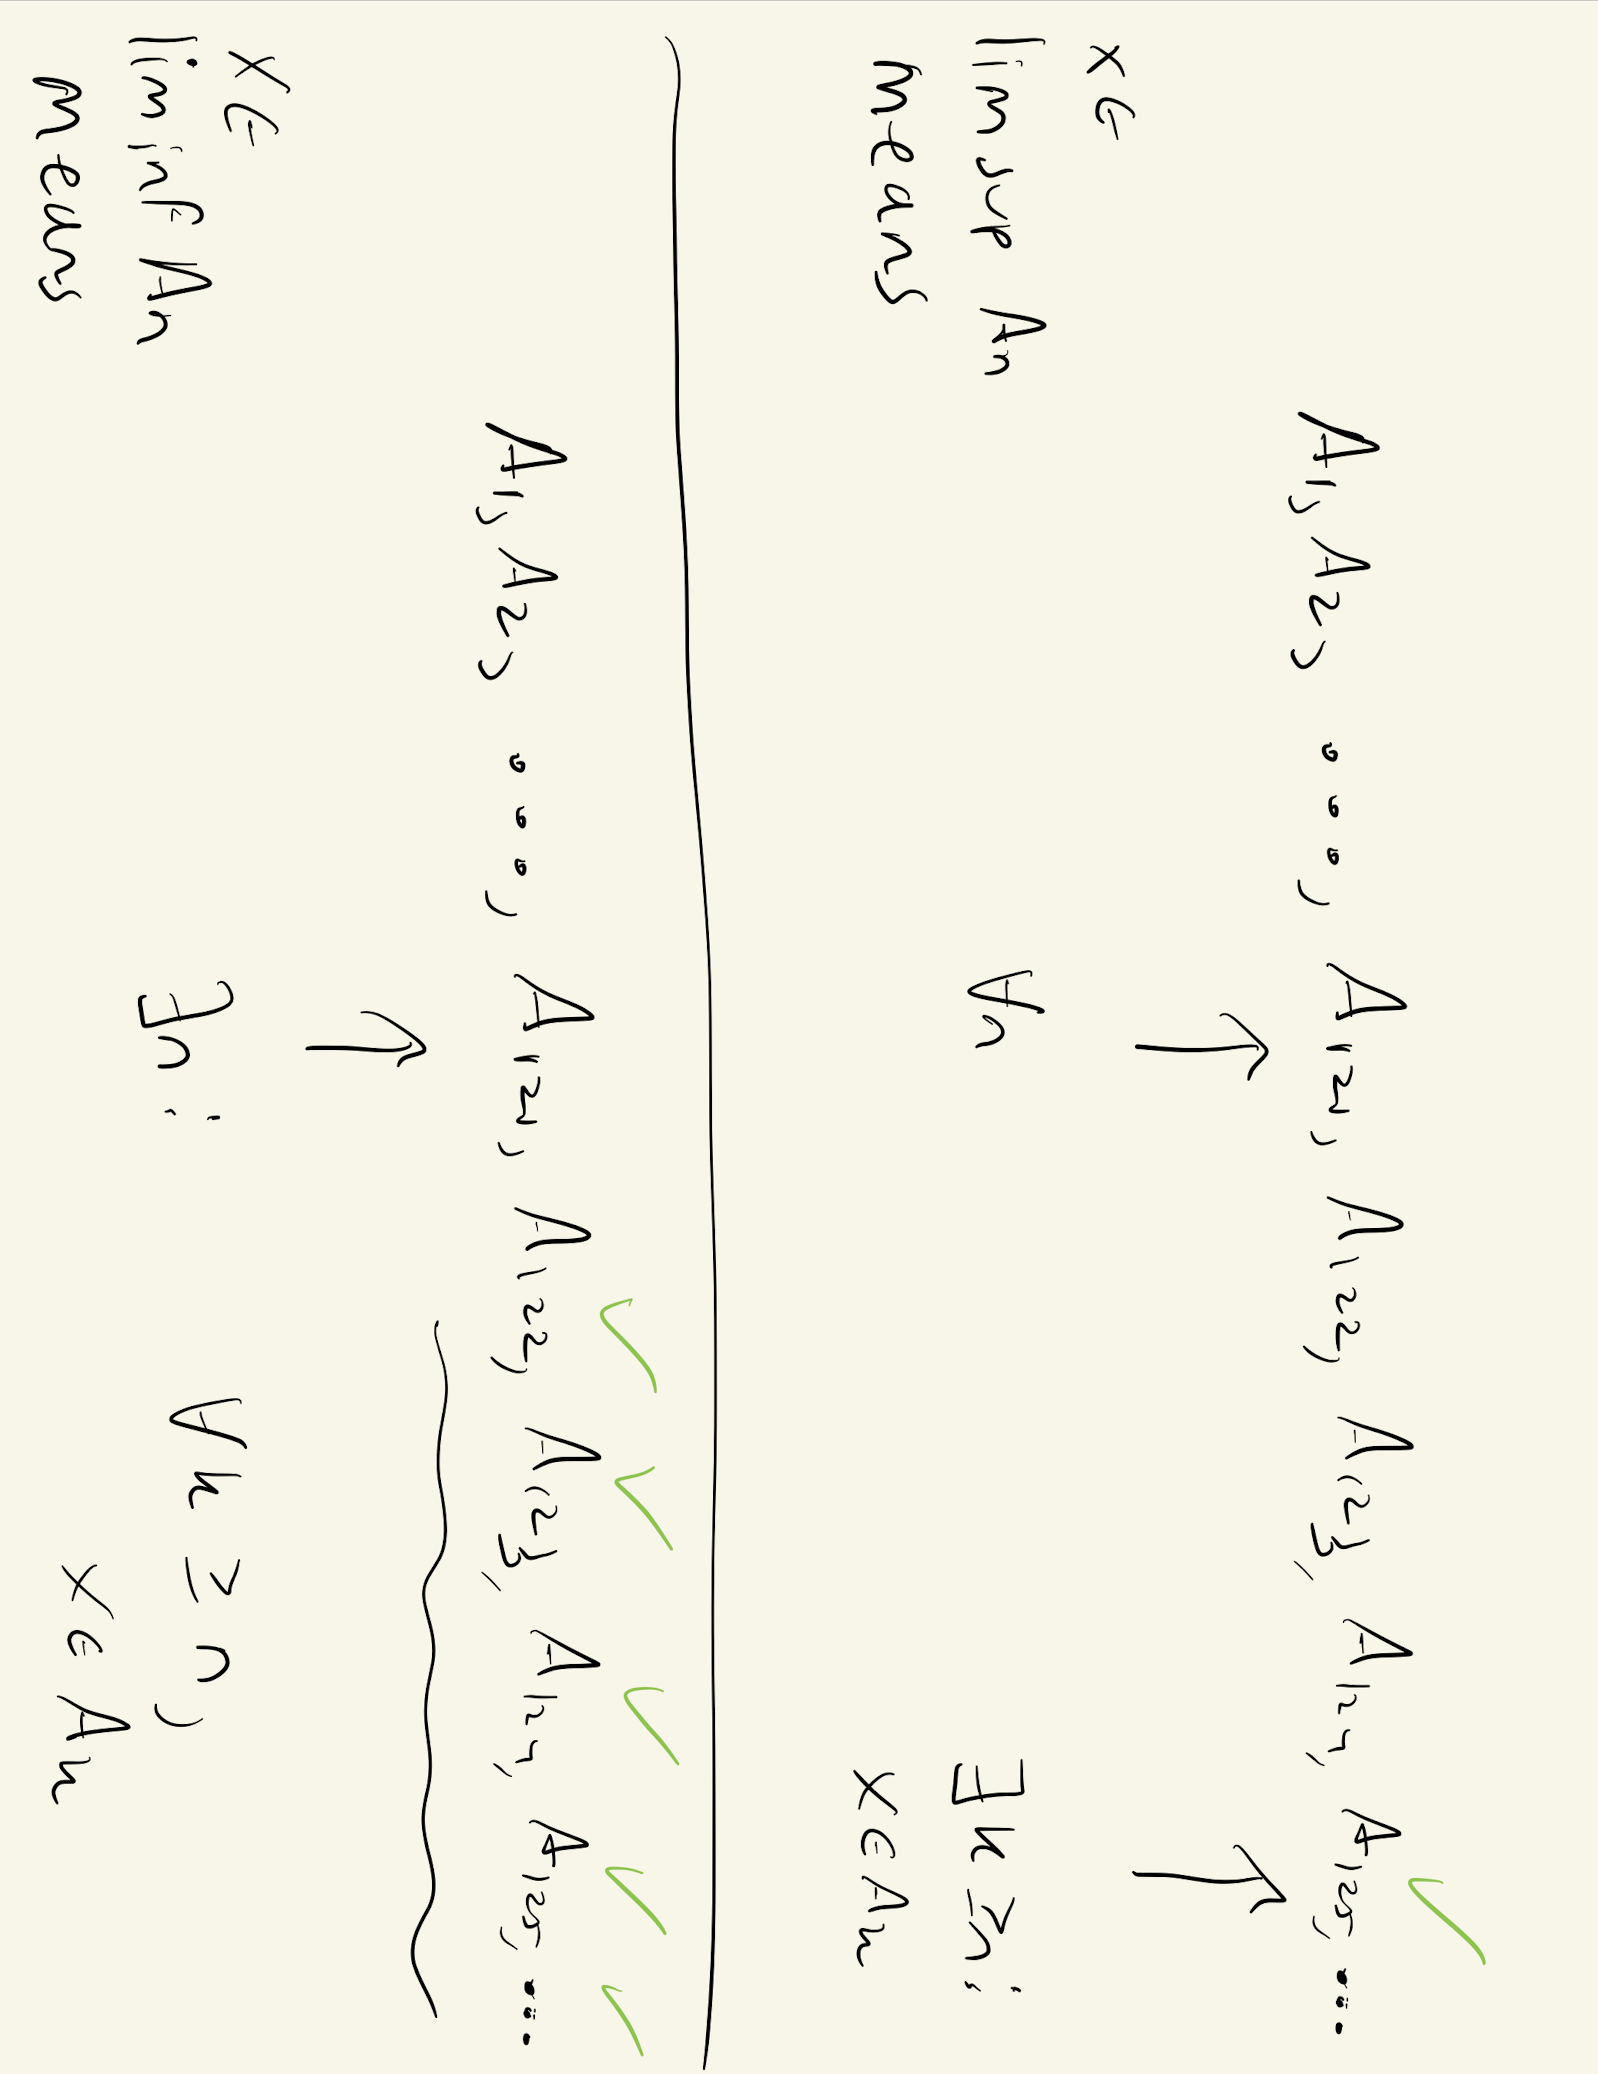
\includegraphics[angle=90, width=.6\textwidth]{images/limsup_and_liminf_of_sets}
\end{figure}

\begin{example}{\remarktitle{A sequence of sets with empty lower limit and non-empty upper limit.}}

\begin{figure}[H]
\centering 
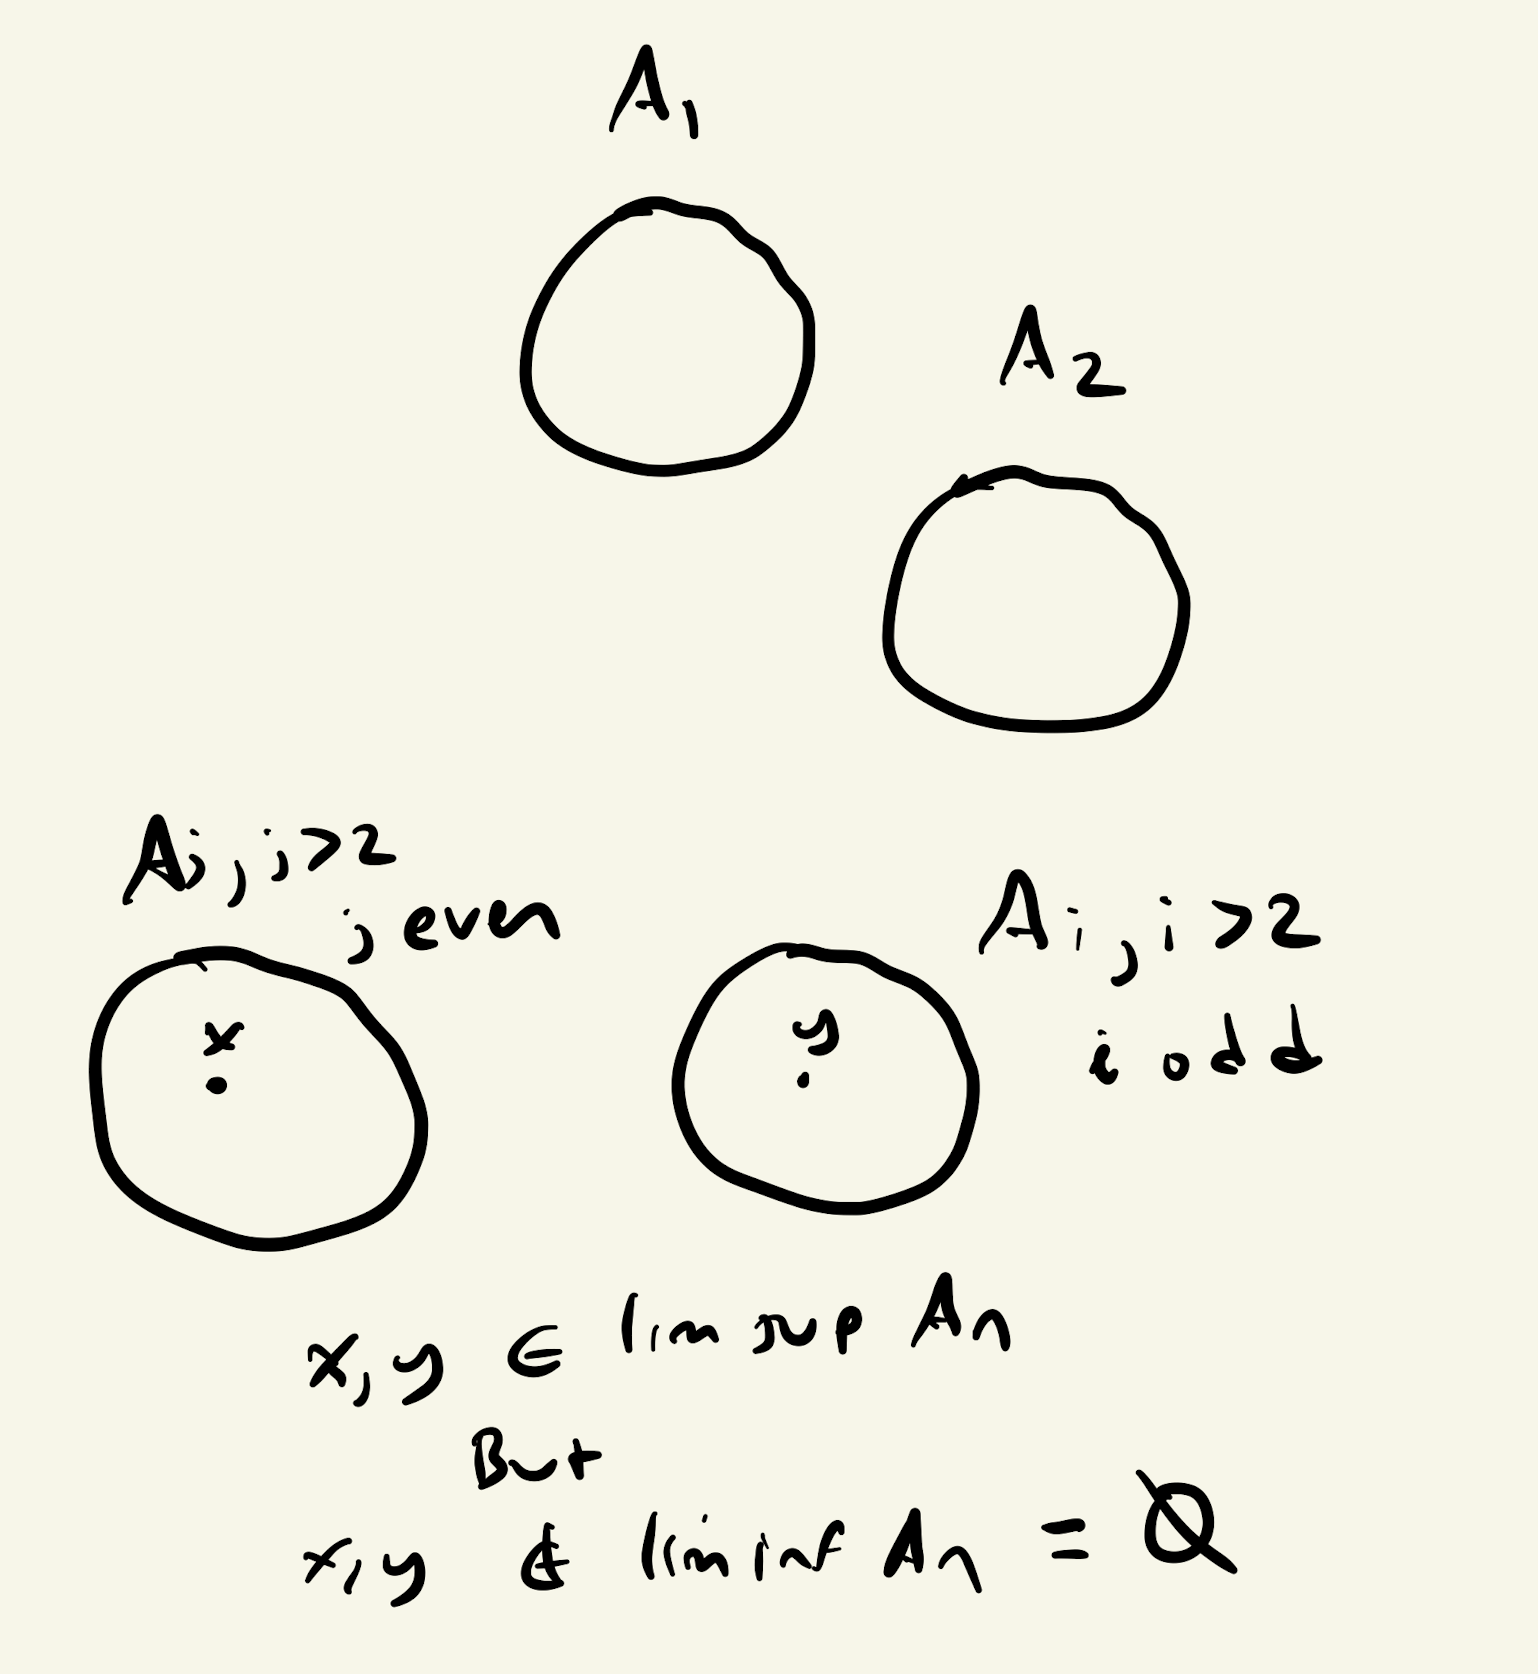
\includegraphics[width=.5\textwidth]{images/limsup_and_liminf_of_sets_example}
\caption{A sequence of sets with empty lower limit and non-empty upper limit.}
\end{figure}

\end{example}

%\begin{discussion}
%Discuss why the two characterizations of upper limit and lower limit are equivalent.	
%\end{discussion}

\begin{definition}
If $\lim\inf A_n = \lim\sup A_n = A$, then A is called the \textbf{limit} of the sequence $A_1, A_2, ...$. 
\end{definition}

\begin{figure}[H]
\centering 
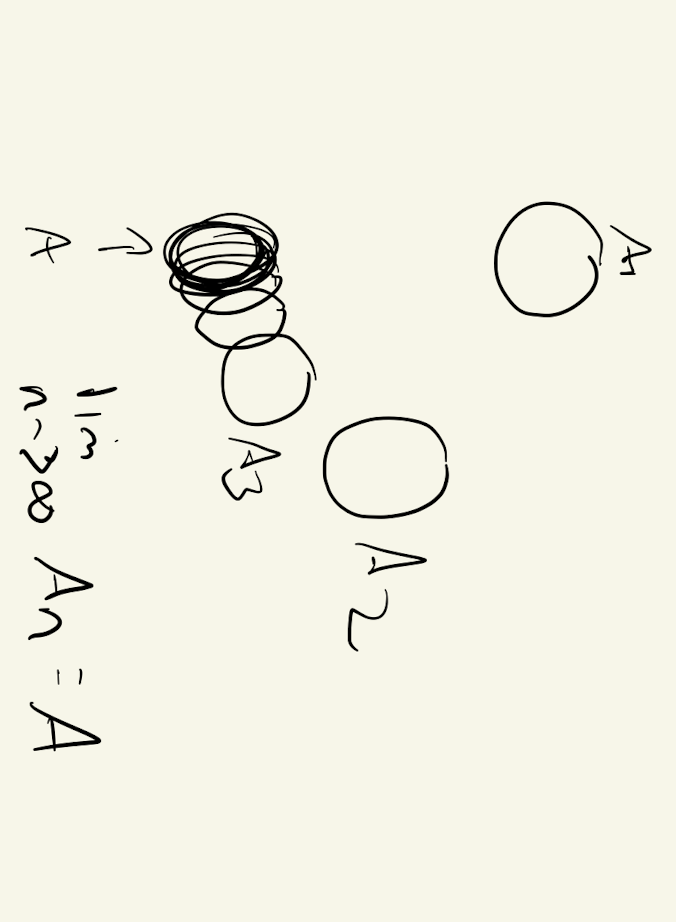
\includegraphics[angle=90, width=.5\textwidth]{images/sequence_of_sets_with_limit}
\caption{A sequence of sets with a limit.}
\end{figure}

Now we present a particular kind of limit that will be useful when we discuss continuity of measure. 

\begin{definition}
If $A_1 \subset A_2 \subset ...$ and $\cup_{n=1}^\infty A_n = A$, we say that the $A_n$ form a \textbf{increasing} sequence of sets with limit $A$ or that the $A_n$ increase to $A$; we write $A_n \uparrow A$.  If $A_1 \supset A_2 \supset ... $ and  	$\cap_{n=1}^\infty A_n = A$, we say that the $A_n$ form a \textbf{decreasing} sequence of sets with limit $A$ or that the $A_n$ decrease to $A$; we write $A_n \downarrow A$.
\end{definition}


\begin{figure}[H]
\centering 
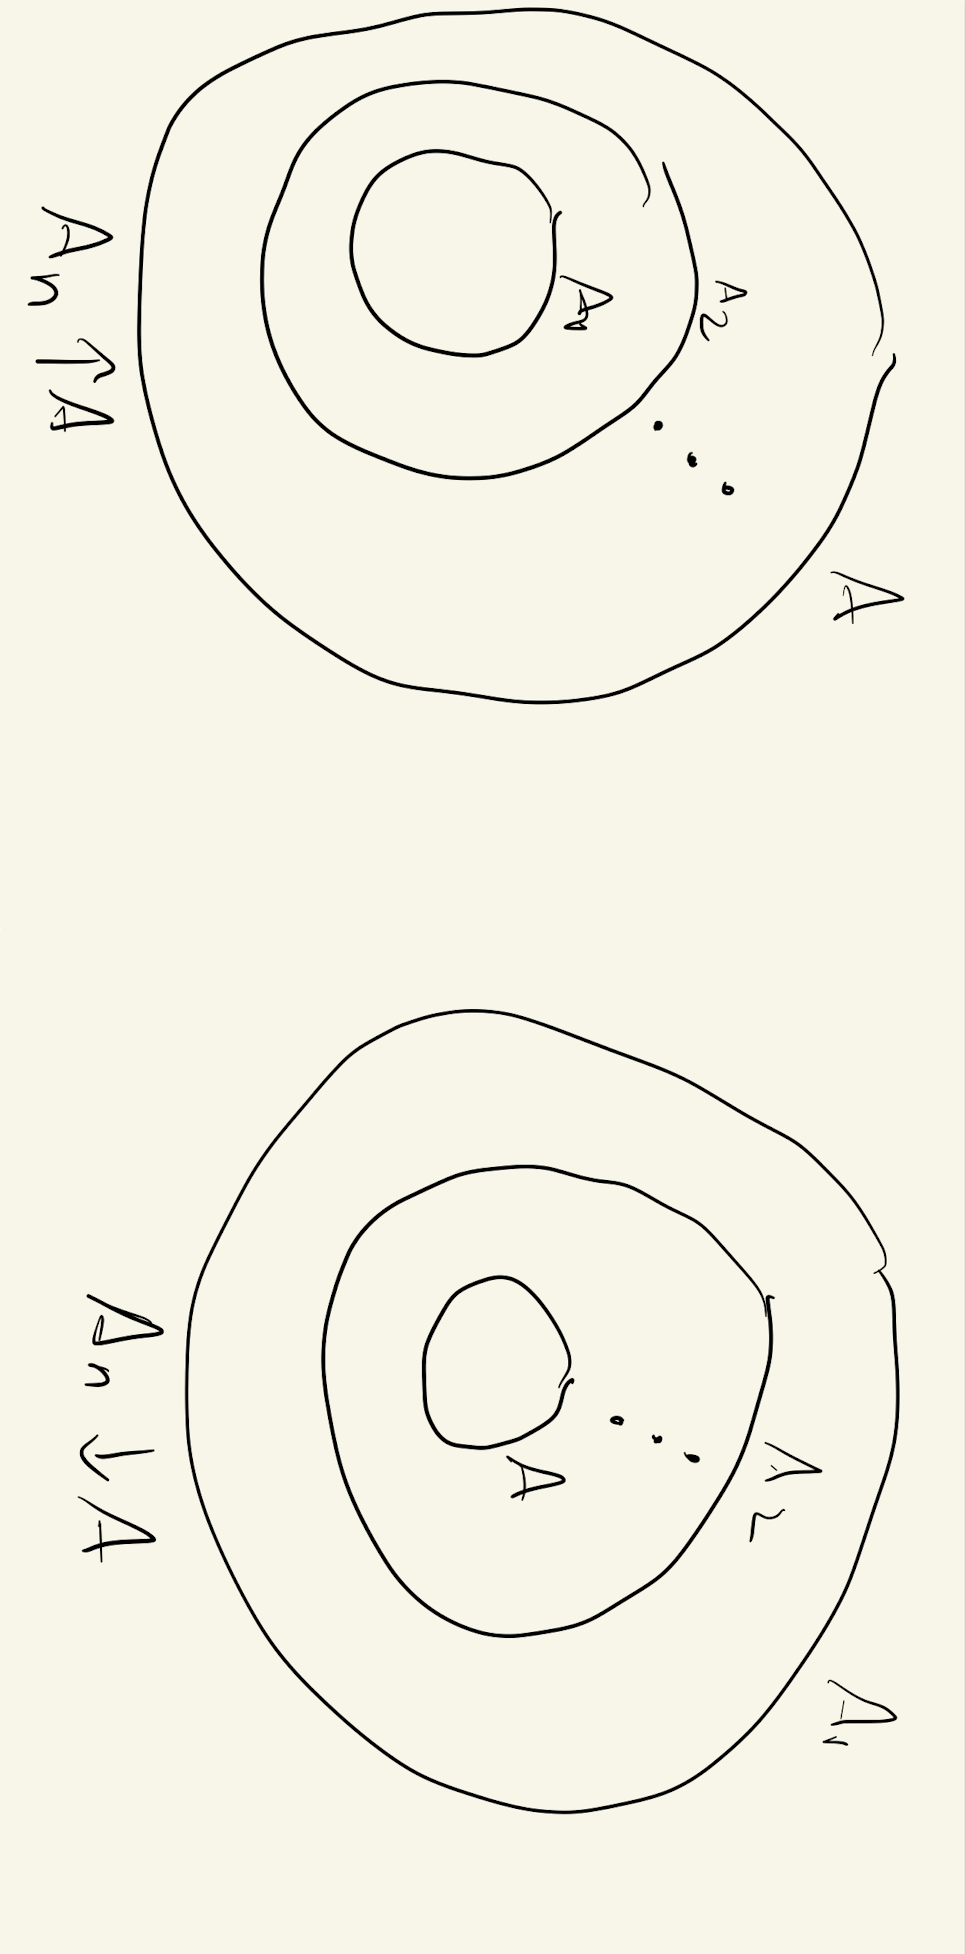
\includegraphics[width=.4\textwidth, angle=90]{images/increasing_and_decreasing_sequence_of_sets}
\caption{An increasing and decreasing sequence of sets.}
\label{fig:increasing_and_decreasing_limits_of_sets}
\end{figure}

One can verify that this definition is consistent with the definition of limits, i.e.
\[  \text{If } A_n \uparrow A \text{ or } A_n \downarrow A \text{ then } \lim\inf A_n = \lim\sup A_n = A.\]

{\tiny For instance, let $A_n \uparrow A$.  So $A_1 \subset A_2  \subset \hdots$ and $A =\bigcup_{n=1}^\infty A_n$. 

Then
\begin{align*} 
\lim\inf A_n &= \bigcup_{n=1}^\infty \bigcap_{k \geq n}^\infty A_k  \stackexplain{containment}{=} \bigcup_{n=1}^\infty  A_n  \stackexplain{def.}{=} A 
\intertext{and}
\lim\sup A_n &= \bigcap_{n=1}^\infty \bigcup_{k \geq n}^\infty A_k  \stackexplain{containment}{=} \bigcap_{n=1}^\infty \bigcup_{k =1}^\infty A_k  \stackexplain{constant}{=} \bigcup_{k =1}^\infty A_k \stackexplain{def.}{=} A 
\end{align*}
So if $A_n \uparrow A$, then $\lim\inf A_n= \lim\sup A_n = A$, i.e. the sequence of sets has a limit, and we write   $A= \lim_{n} A_n$.
}


As shown in Figure \ref{fig:increasing_and_decreasing_limits_of_sets}, limits of increasing and decreasing sequences are very special kinds of limits.


\subsection{Representing unions as disjoint unions} \label{sec:representing_unions_as_disjoint_unions}
 
\begin{remark}
If $A_1,A_2,...$ are subsets of some set $\Omega$, then
\begin{align*} 
\bigcup_{n=1}^\infty A_n = \bigcupdot_{n=1}^\infty \bigg(A_n \cap A_{n-1}^c \cap ... \cap A_1^c \bigg) 	
\labelit \label{eqn:union_as_disjoint_union}
\end{align*}

In other words, any union can be re-represented as a disjoint union. This is useful because measures are countably additive on disjoint sets, so we prefer to work with collections of disjoint sets.
\label{rk:rerepresenting_unions_as_disjoint_unions}
\end{remark}

\begin{remark}
If $A_n \uparrow A$, then \eqref{eqn:union_as_disjoint_union} becomes
\begin{align*}
	\bigcup_{n=1}^\infty A_n = \bigcupdot_{n=1}^\infty \bigg( A_n - A_{n-1} \bigg) 
\labelit \label{eqn:union_as_disjoint_union_for_increasing_sequences}
\end{align*}
This is because $A_{n-1} \subset A_{n}$, so $A_{n-1}^c \supset A_{n}^c$ by contraposition.	
\end{remark}

\section{$\S$ 1.2: Fields, \sfs, measures}

\subsection{$\S$ 1.2.1-1.2.2: Fields and \sfs}

Probability measures, and measures more generally, cannot be defined on all subsets of many spaces that we would like to deal with.  For instance, non-measurable sets can be shown to exist even for Lebesgue measure on the unit interval.  Proposition 1.2.6 of \cite{rosenthal2006first} shows that there is no definition of $P(A)$ that is defined for all subsets $A \subseteq [0,1]$ satisfying all three conditions below\footnote{In Proposition \ref{prop:existence_of_set_that_is_not_Lebesgue_measurable}, we make a similar observation, along with a proof: there cannot be a measure defined on all subsets of the reals that is both translation invariant and has a finite value on all bounded intervals.}
\begin{enumerate}
\item $P([a,b]) = b-a, \quad 0 \leq a \leq b \leq 1$.	
\item $P(\bigcupdot_{n=1}^\infty A_n ) = \ds\sum_{n=1}^\infty P(A_n)$ for $A_1, A_2, ...$ disjoint subsets of $[0,1]$.
\item $P(A \bigoplus r) = P(A), \quad 0 \leq r \leq 1$, where $A \bigoplus r$ denotes the \textit{r-shift} of $A$, i.e. 
\[ A \bigoplus r := \set{a+r : a \in A, a+r \leq 1} \cup \set{a+r-1 : a \in A, a +r >1}\]
\end{enumerate}
In Sec.~\ref{sec:set_that_is_not_Lebesgue_measurable}, we provide more information about a set that is not Lebesgue measurable.

The solution to this problem is to define measures on a restricted domain, $\sigma$-fields.

\subsubsection{$\sigma$-fields}



%We begin with a discussion of $\sigma$-fields, which are typically the domains of probability measures, and measures more generally.\footnote{In the construction of Lebesgue measure, Ash defines a probability measure on a field.  See 1.3.1 of \cite{ash2000probability}.}  As stated in the motivation (Section \ref{sec:motivation_for_topic}), measures cannot be defined on all subsets of many spaces that we would like to deal with. 

%\sfs\ are important because they are the domain of measures.  
%Here are some definitions.

\begin{definition}
Let $\F$ be a collection of subsets of a set $\Omega$.  Then $\F$ is called a \textbf{sigma-field} (or \textit{sigma-algebra}) if it satisfies

\begin{enumerate}[label=\alph*)]
	\item $\Omega \in \F$ 
	\item If $A \in \F$, then $A^c \in \F$.
	\item If $A_1,A_2, ... \in \F$ then $\cup_{i=1}^\infty A_i \in \F$.  
\end{enumerate}
that is, if $\Omega \in \F$ and $\F$ is closed under complementation and countable unions.
\label{def:sigma_field}	
\end{definition}

\begin{remark}
It follows that $\sigma$-fields are closed under countable intersections, since
\[ \cap_{i=1}^\infty A_i \stackrel{\text{DeMorgan's Law}}{=} (\cup_{i=1}^\infty A_i^c)^c \]	
\end{remark}

\begin{example}
$\F =\set{\emptyset, \Omega}$ is the smallest \sf\ on $\Omega$. 
\end{example}

\begin{example}
	$\F =2^\Omega$, i.e. the set of all subsets of $\Omega$, is the largest \sf\ on $\Omega$.
\label{ex:the_largest_sigma_field_is_the_power_set}
\end{example}

\begin{example}
If $A \in \Omega$ is non-empty, then $\F = \set{\emptyset, A, A^c, \Omega}$ is the smallest \sf\ containing $A$.
\end{example}

\begin{notation}
If $\C$ is a class of sets, the smallest \sf\ containing the sets of $\C$ is written as $\sigma(\C$).  This is sometimes called the \textit{minimal \sf\ over $C$} or the \textit{\sf\ generated by $C$}. 
\end{notation}
	
\begin{problem}{\remarktitle{\cite{ash2000probability} Problem 1.2.8}}
\label{prob:minimal_sigma_field_containing_n_subsets}
Let $A_1,...,A_n$ be subsets of $\Omega$.  Describe $\F := \sigma(\set{A_1,...,A_n})$, the smallest \sf\ containing $A_1,...,A_n$.  Also describe the number of sets in $\F$.    
\end{problem}

\begin{proof}[Solution]
We can derive the strict upper bound $|\F| \leq 2^{2^n}$. For a complete answer, see GoodNotes. 	

The gist is that the collection $\set{A_1,...,A_n}$ partitions $\Omega$ into up to $M=2^N$ pieces, and the minimal sigma field contains all possible finite unions of these pieces, so has at most $2^{M}$ elements.
  
\begin{figure}[h!]
\centering 
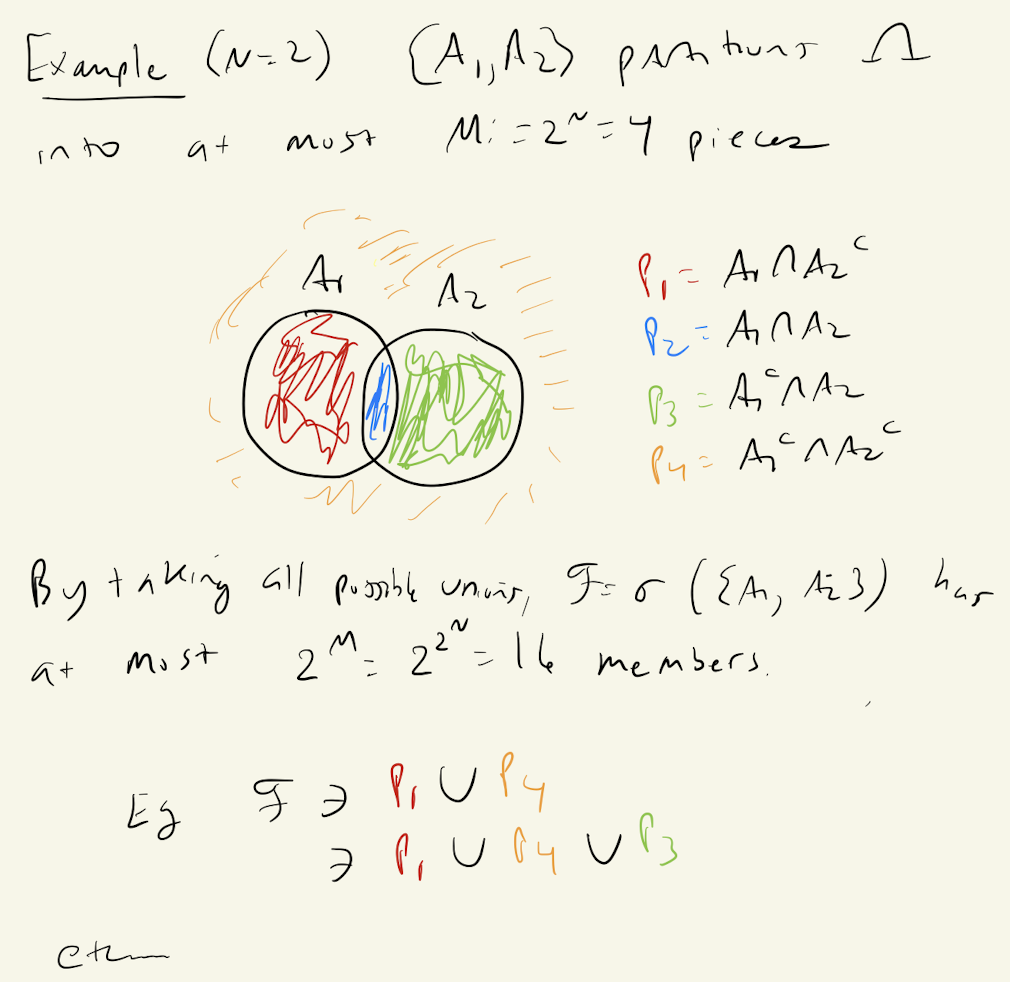
\includegraphics[width=.7\textwidth]{images/minimal_sigma_fields}
%\caption{An increasing and decreasing sequence of sets, followed by a sequence of sets which is neither, but which has a limit.}
\end{figure}

\end{proof}

\subsubsection{Fields}

Fields are more general than $\sigma$-fields.  Measures are sometimes constructed by being defined on fields, and then extended to \sfs.  Indeed, we will see this strategy with Lebesgue measure. 

\begin{definition}
Let $\F$ be a collection of subsets of a set $\Omega$.  Then $\F$ is called a \textbf{field} (or \textit{algebra})  if satisfies Definition \ref{def:sigma_field} after replacing condition c) with

\begin{enumerate}
	\item[c')] If $A_1,...A_n \in \F$ then $\cup_{i=1}^n A_i \in \F$.
\end{enumerate}
that is, if $\Omega \in \F$ and $\F$ is closed under complementation and \textit{finite} unions.
\label{def:field}	
\end{definition}

\begin{example} What is an example of a collection that is a \textit{field}, but not a $\sigma$-\textit{field}?  

Let $\Omega=\R$ and $\F_0 = \set{\text{finite disjoint unions of right semi-closed intervals } (a,b], a \neq b}$.\footnote{By convention, we also count $(a, \infty)$ as right semi-closed for $-\infty\leq a < \infty$, which is necessary for the \sf\ to be closed under complements. See Def.~\ref{def:rsc_intervals}.}    Then $\F_0$ is a field, as can be motivated graphically (or see Remark~\ref{rk:the_collection_of_disjoint_unions_of_right_semi_closed_rectangles_is_a_field} for a precise argument). 

\begin{figure}[H]
\centering
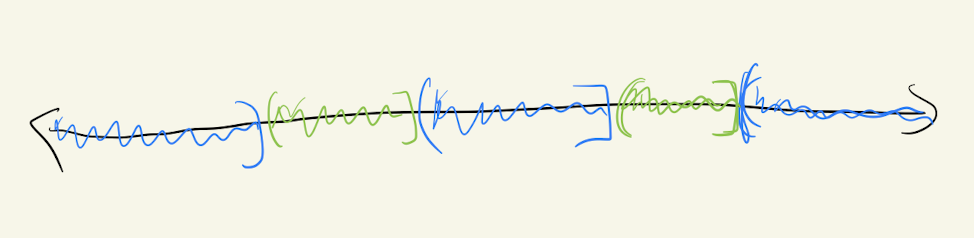
\includegraphics[width=.6\textwidth]{images/rsc_intervals}	
\end{figure}

But $\F_0$ is \underline{not} a \sf.  

\ifActive 
\textbf{Workshop Exercise}: Prove this.
\else 
Note that if $A_n = (-\frac{1}{n},0]$, then $\bigcap_{n=1}^\infty A_n = \set{0}  \not\in \F_0$.
\fi 

\label{ex:field_of_finite_disjoint_unions_of_rsc_intervals}
\end{example}

Now we give a simple way to form fields \cite[pp. 23]{folland1999real}.  We do this in Prop.~\ref{prop:from_elementary_families_to_fields}. First, a definition. 

\begin{definition}
An \textbf{elementary family} is a collection $\scriptE$ of subsets of $\Omega$ such that 
\begin{alphabate}
\item $\emptyset \in \scriptE$
\item if $E,F \in \scriptE$ then $\scriptE \cap \F \in \scriptE$
\item if $E \in \scriptE$, then $E^c$ is a finite disjoint union of members of $\scriptE$.	
\end{alphabate}
\label{def:elementary_family}
\end{definition}

\begin{proposition}
If $\scriptE$ is an elementary family then the collection 
\[ \F_0 := \set{ \text{finite disjoint unions of members of } \scriptE} \]
is a field.
\label{prop:from_elementary_families_to_fields}	
\end{proposition}

\begin{proof}
See \cite[pp.24]{folland1999real}.
\end{proof}

\begin{remark}{\remarktitle{The collection of disjoint unions of right semi-closed rectangles is a field.}}
By Prop.~\ref{prop:from_elementary_families_to_fields}, it is sufficient to show that the right semi-closed rectangles $\set{(a,b], a \neq b}$ (see Def.~\ref{def:rsc_intervals} for a precise definition) are an elementary family.  So we verify the conditions:

\begin{alphabate}
\item $\emptyset \in \scriptE$ ? \greencheck. Take $b<a$.
\item if $E,F \in \scriptE$ then $\scriptE \cap \F \in \scriptE$ ? \greencheck.  Let $E = (a_1, b_1]$ and $F= (a_2, b_2]$.   
	\begin{itemize}
	\item If $a_2 \geq b_1$, then $E \cap F = \emptyset  \explaintermbrace{by (a)}{\in \scriptE}.$
	\item If $a_2 < b_1$, then $E \cap F = (a_2, b_1] \explaintermbrace{by def rsc intervals}{\in \scriptE}.$
	\end{itemize}
\item if $E \in \scriptE$, then $E^c$ is a finite disjoint union of members of $\scriptE$ ?	\greencheck.  If $E = (a,b]$, then 
\[  E^c  = \explaintermbrace{$\in \scriptE$ by def r.s.c}{(-\infty, a]} \cup  \explaintermbrace{$\in \scriptE$ by a technicality; see Def.~\ref{def:rsc_intervals} }{(b, \infty)}\]
\end{alphabate}
\label{rk:the_collection_of_disjoint_unions_of_right_semi_closed_rectangles_is_a_field}	
\end{remark}



\begin{remark}
 If $\F$ is a field, a countable union of sets in $\F$ can be expressed as the limit of an increasing sequence of sets in $\F$, and conversely. For if $A_n \in \F$ and $A_n \uparrow A$, then A is a countable union of sets in $\F$ by definition.  Conversely, if $A = \cup_{n=1}^\infty A_n$, then set $B_N := \cup_{n=1}^N A_n$ and $B_N \uparrow A$. This shows that a \sf\ can also be described as a field that is closed under limits of increasing sequences.  More generally, if $\G$ is the collection of all limits of increasing sequences of sets in some field $\F_0$, we can also describe $\G$ as the collection of all countable unions of sets in $\F_0$. \label{rk:the_limits_of_increasing_and_decreasing_sequences_of_sets_in_a_field_are_also_the_countable_unions}
\end{remark}
%Recalling Figure \ref{fig:increasing_and_decreasing_limits_of_sets}, limits of increasing sequences are very special kinds of limits.


\subsubsection{``Good sets" strategy} \label{sec:good_sets_strategy}

Ash says that there is a type of reasoning that occurs so often in problems involving \sfs\ that it deserves explicit mention.  It is called the \textit{good sets strategy}.   Suppose you want to show that all members of a $\sigma$-algebra   $\F$ have some property $P$.  Define ``good sets" as those that satisfy the property
\[ \G := \{ G \in \F : G \text{ has property } P \} \]
The strategy is then to simply
\begin{enumerate}
\item Show $\G$ contains some class $\C$ such that $\F = \sigma(\C)$
\item Show $\G$ is a $\sigma$-algebra 	
\end{enumerate}


Then you're done!  

Why does this work?

\begin{align*}
& \quad \C \subset \G &&	\text{by 1}\\
&\implies \sigma(\C) \subset \sigma(\G) &&  \\
&\implies \F \subset \G && \text{by 1,2} \\
& \text{Yet $\G \subset \F$ by definition of $\G$.} && \\
& \text{So $\G = \F$.} && \\
& \text{ So all sets in $\F$ are good.} && \\
\end{align*}

Some example applications:
 \begin{itemize}
 \item In the text, Ash uses this strategy (see pp.5) to show that if $\C$ is a class of subsets of $\Omega$, and $A \in \Omega$, then

\[ \explaintermbrace{take minimal sigma field first, then intersect}{\sigma_\Omega(\C) \cap A} = \explaintermbrace{intersect first, then take minimal sigma-field}{\sigma_A(\C \cap A)} \]
 \item  See my handwritten homework exercise for  $\S$ 1.2, Problem 6.
 \item Sections of measurable sets are measurable.
 %\item See the proof of Caratheodory Extension Theorem (Theorem \ref{thm:caratheodory_extension}).	
 \end{itemize}

\begin{remark} 
Later, we will cover the Monotone Class Theorem (see Theorem \ref{thm:monotone_class_theorem}), which provides an alternate mechanism for executing the Good Sets Strategy.  See Remark \ref{rk:monotone_class_theorem_for_executing_good_sets_strategy}.
\end{remark}

\subsubsection{Borel Sets} \label{sec:borel_sets}

An important example of a $\sigma$-field is the Borel Sets $\B(\R)$, defined as the smallest \sf\ of subsets of $\R$ containing all right semi-closed intervals $(a,b] \subset \R$.  

We may alternately characterize $\B(\R)$ as the smallest \sf\ containing
\begin{alphabate}
\item all intervals $(a,b], \; a,b \in \R$
\item all intervals $(a,b), \; a,b \in \R$
\item all intervals $[a,b), \; a,b \in \R$
\item all intervals $[a,b], \; a,b \in \R$.
\item all intervals $(a,\infty), \; a \in \R$.
\item  all intervals $[a,\infty), \; a \in \R$.
\item 	 all intervals $(-\infty,b), \; b \in \R$.
\item  all intervals $(-\infty,b], \; b \in \R$.\footnote{Let $a \in \R$. Intervals of the form $(a, \infty)$ or $(-\infty, a)$ are called open rays.  Intervals of the form $[a, \infty)$ or $(-\infty, a]$  are called closed rays.}
\item all open sets of $\R$.\footnote{Recall that an open set is a countable union of open intervals.}
\item all closed sets of $\R$.\footnote{Recall that a set is open iff its complement is closed.}
\end{alphabate}

\ifActive 
\textbf{Workshop Exercise}: Justify that (a) and (b) are equivalent. 
\else 
To illustrate these equivalences, let us equate the first two conditions. That is, let us show that a \sf\ contains all open intervals $(a,b)$ iff it contains all right semi-closed intervals $(a,b]$.  To see this, simply note
\begin{subequations}
\begin{align}
(a,b] &= \bigcap_{n=1}^\infty \bigg(a, b+\frac{1}{n}\bigg) \\
	\intertext{and}
(a,b) &= \bigcup_{n=1}^\infty \bigg(a, b-\frac{1}{n}\bigg] 
\end{align}
\label{eqn:open_intervals_as_rsc_intervals_and_vice_versa}
\end{subequations}
{\tiny For example, the first equation in \eqref{eqn:open_intervals_as_rsc_intervals_and_vice_versa} can be verified by the argument 
\[x \in  \bigcap_{n=1}^\infty \bigg(a, b+\frac{1}{n}\bigg) \iff x \in (a,b-\frac{1}{n}) \; \forall n \iff x>a \; \text{and} \; x < b -\frac{1}{n} \; \forall n \iff x >a \; \text{and} \; x \leq b \iff x \in (a,b] \]
.}

\fi 




\begin{question}
The text gives another description of the Borel sets $\B(\R)$ as the smallest \sf\ containing $\F_0$, the field of disjoint unions of right semi-closed intervals $(a,b]$.  Can we make the same statement about the field of finite disjoint unions of left semi-closed intervals?
\end{question}

The Borel sets are a large collection of sets.  For instance, Remark \ref{rk:cantor_set_is_a_borel_set} notes that the Cantor set is a Borel set. 

\begin{remark}{\remarktitle{The Cantor set is a Borel set}}
The Cantor set must be a Borel set because it is closed.  To see this more explicitly, note that in each step you "remove the middle third of each part".  
\[K = \bigcap_{i=1}^\infty\bigcap_{j=1}^{3^{i-1}-1}\left[0,\frac{3j+1}{3^i}\right]\cup \left[\frac{3j+2}{3^i}, 1\right] \]
which is a countable number of intersections and unions of closed intervals, and hence Borel by characterization (d) above. 
\label{rk:cantor_set_is_a_borel_set}
\end{remark}

\subsection{$\S$ 1.2.3-1.2.4: Measures}




\begin{definition}
A \textbf{measure} on a \sf\ $\F$ is a non-negative, extended real-valued function $\mu$ on $\F$ such that whenever $A_1, A_2, ...$ form a finite or countably infinite collection of disjoint sets in $\F$, we have countable additivity; that is,
\[ \mu \bigg( \bigcupdot_n A_n \bigg) = \ds\sum_n \mu(A_n) \]
\label{def:measure}	
\end{definition}

\begin{definition}
A \textbf{probability measure} is a measure (Definition \ref{def:measure}) where $\mu(\Omega)=1$.
\label{def:prob_measure}		
\end{definition}

\begin{remark}
Ash additionally assumes that a measure does not take $\mu(A) = \infty$ for all $A \in \F$.\footnote{Likewise, he assumes that signed measures do not take $\mu(A) = -\infty$ for  for all $A \in \F$.}  From this, we automatically obtain $\mu(\emptyset)=0$. For $\mu(A) < \infty$ for some $A$, and by considering the sequence $A, \emptyset, \emptyset, ...$, we have that $\mu(\emptyset)=0$ by countable additivity.   	
\end{remark}

\begin{example}
Let $\Omega$ be any set.  Fix $x_0 \in \Omega$.  Let $\F = 2^\Omega$.  For any $A \in \F$ define $\mu(A) = 1$ if $x_0 \in A$ and $\mu(A) = 0$ if $x_0 \not\in A$.  Then $\mu$ may be called the \textbf{unit mass} concentrated at $x_0$.
\end{example}

\begin{example}
Let $\Omega = \set{x_1,x_2,...}$ be a finite or countably infinite set.  Let $p_1, p_2,...$ be non-negative reals.  Let $\F = 2^\Omega$.  Define
\[\mu(A) = \ds\sum_{x_i \in A} p_i \quad \text{ for all } A \in \F\]
Then $\mu$ is a measure on $\F$. We might call it the ``point weighting" measure. 
\begin{itemize}
\item If $p_i \equiv 1 \; \forall \, i$, then $\mu$ is called the \textbf{counting measure}. (It gives the number of points in $A \subset \Omega$.)
\item If $\sum_i p_i =1$, then $\mu$ is a discrete probability measure.	
\end{itemize}
	
\end{example}


\begin{example}{\remarktitle{Lebesgue measure}}
Define $\mu$ such that 
\[ \mu(a,b] = b-a \quad \forall \, a,b \in \R : b>a \]
As we will see in Section \ref{sec:extension_of_measures}, this requirement determines $\mu$ on a large collection of sets, the Borel Sets $\B(\R)$, which we defined in Section \ref{sec:borel_sets} as the smallest \sf\ of subsets of $\R$ containing all intervals $(a,b] \subset \R$. 
\label{ex:Lebesgue_measure}
\end{example}


\subsection{$\S$ 1.2.5-1.2.6: Properties of measures (and some more general set functions)}

The text considers some generalizations of measures that can be obtained
\begin{enumerate}
\item  by restricting the domain to a field {\footnotesize (in other texts, such functions are called \textit{pre-measures}) }
\item  by only assuming \textit{finite} additivity 
\item by allowing the range to be extended reals ($\bar{\R}$) instead of non-negative extended reals ($\bar{\R}_{\geq 0}$).  
\end{enumerate}



\begin{remark}
With respect to pre-measures, a countably additive function can be defined on a \textit{field} (rather than \sf) if the condition is taken to hold whenever a countable union \textit{does} happen to still be in the field.  Unless otherwise specified, I will assume in these notes by that countably additive functions are always defined on \sfs, and finitely additive functions are defined on fields.
\label{rk:i_am_assuming_a_domain_based_on_the_type_of_additivity}
\end{remark}	



\begin{table}[!h]
\centering	
\begin{tabular}{rcc}
&\multicolumn{2}{c}{\textbf{Range}} \\
& \textbf{non-negative extended reals} & \textbf{extended reals} \\
\textbf{countably additive}& $\mu$ measure  & $\tilde{\mu}$ signed measure \\
\textbf{finitely additive}& $\mu_0$ & $\tilde{\mu}_0$ \\	
\end{tabular}
\caption{Notation for generalizations of measure (For assumed domain in each case, see Remark \ref{rk:i_am_assuming_a_domain_based_on_the_type_of_additivity}.)}
\label{tab:notation_for_generalizations_of_measure}
\end{table}

In Table \ref{tab:notation_for_generalizations_of_measure},  we introduce some notation to try to clarify more immediately when results hold. Note the relations\footnote{So, for example, if something holds for $\tilde{\mu}_0$, it holds for $\mu$.  A simple mnemonic is that adding stuff to the notation generalizes the function.}  
\[ \set{\mu} \subset \set{\mu_0}, \set{\tilde{\mu}} \subset \set{\tilde{\mu}_0}. \]

\begin{remark}
Being able to work with these generalizations will be important in Section \ref{sec:extension_of_measures} on extension of measures.  In particular, it will help us show that we can construct the Lebesgue measure on the Borel sets.
\end{remark}

 \begin{example} Let $\F_0$ be the field of finite disjoint unions of right semi-closed intervals (see Definition \ref{def:rsc_intervals} ), and define the set function $\fasf$ on $\F_0$ as follows\footnote{This example comes from Problem 4 in Section 1.2 of the text}:

\begin{align*}
\fasf(-\infty,a] &=a, && a \in \R  \\
\fasf(a,b] &= b-a, && a,b \in \R, \quad a<b  \\
\fasf(b, \infty) &= -b, && b \in \R \\
\fasf(\R) &=0 &&\\
\fasf(\bigcupdot_{i=1}^n I_i) &= \sum_{i=1}^n \fasf(I_i), && \text{if $I_1, ..., I_n$ are right semi-closed intervals} 
\end{align*}
	
Then $\fasf$ is finitely additive, but not countably additive on $\F_0$.  (Why?) For a proof, see GoodNotes.
 \end{example}

 
Measure-like set functions have useful properties. Using the notation in Table \ref{tab:notation_for_generalizations_of_measure}, we rewrite Theorem 1.2.5 of the text:
 
 \begin{theorem}
 Let $\fasf$ be a finitely additive set function on the field $\F_0$.  Then
 \begin{enumerate}[label=\alph*)]
 \item \label{itm:first} $\fasf(\emptyset)=0$
 \item \label{itm:second} $\fasf(A \cup B) + \fasf (A \cap B) = \fasf(A) + \fasf(B)$ for all $A,B \in \F_0$.
 \begin{figure}[H]
 \centering
 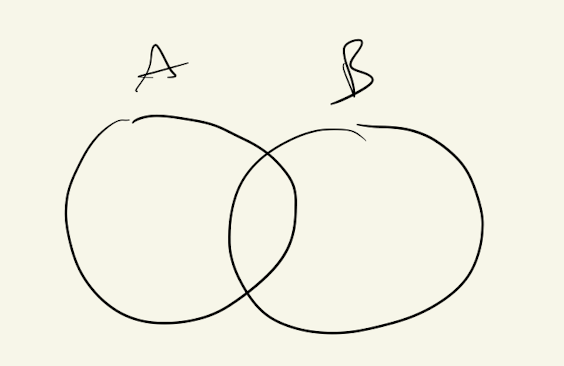
\includegraphics[width=.2\textwidth]{images/two_overlapping_sets}	
 \end{figure}

 \item \label{itm:piece-and-difference} If $A,B \in \F_0$ and $B \subset A$, then   
  \[ \fasf(A) = \fasf(B) + \fasf(A-B)\quad \text{(piece-and-difference decomposition)} \] 
 \begin{figure}[H]
 \centering
 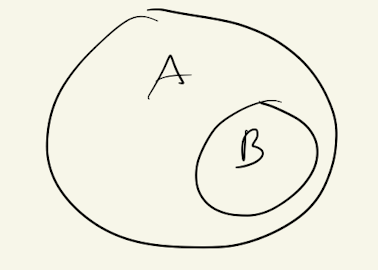
\includegraphics[width=.2\textwidth]{images/whole_and_piece}	
 \end{figure}
 
 \footnote{If the ``piece" satisfies $\fasf(B) < \infty$, we have $\fasf(A-B) = \fasf(A) - \fasf(B) $.  One useful takeaway for piece-and-difference decompositions is that : \textit{the finite measure of the difference is the difference of the finite measures}.}So $\fasf(A) \geq \fasf(B)$ if $\fasf(A-B) \geq 0$. More generally, for non-negative set functions, we have
 \[ \mu_0 (A) \geq \mu_0 (B) \quad \text{(monotonicity)} \] 
 \item \label{itm:subadditivity} Subadditivity holds if $\fasf$ is non-negative, i.e.
 \begin{align*}
 \mu_0 (\cup_{i=1}^n A_i)& \leq \sum_{i=1}^n \mu_0(A_i) \\
  \mu (\cup_{i=1}^\infty A_i)& \leq \sum_{i=1}^\infty \mu(A_i) \\
 \end{align*}
 \end{enumerate}
\label{thm:basic_properties_of_finitely_additive_set_functions}
 \end{theorem}
  
\begin{proof}
 We prove Theorem \ref{thm:basic_properties_of_finitely_additive_set_functions} (b).  The rest is an exercise for the reader (or see the text).
 
 \ifActive 
\textbf{Workshop Exercise}: Prove part (b).
\else 
 First, we break things into disjoint pieces
 {\footnotesize 
\begin{align*}
A &= \bigg(A \cap B \bigg) \, \bigcupdot \, \bigg(A \cap B^c \bigg)	&& \implies \fasf(A) = \fasf (A \cap B) +  \fasf (A \cap B^c)  && (1) \\
B &= \bigg(A \cap B \bigg) \, \bigcupdot \, \bigg(A^c \cap B \bigg)	&& \implies \fasf(B) = \fasf (A \cap B) +  \fasf (A^c \cap B)  && (2) \\
A \cup B &= \bigg(A \cap B \bigg) \, \bigcupdot \, \bigg(A \cap B^c \bigg) \bigcupdot \, \bigg(A^c \cap B \bigg)	&& \implies \fasf(A \cup B) = \fasf (A \cap B) +  \fasf (A \cap B^c) + \fasf (A^c \cap B)   && (3) 
\end{align*}
}

Summing (1) and (2), we obtain
\[\fasf(A) + \fasf(B) = 2 \fasf(A \cap B) + \fasf(A \cap B^c) + \fasf(A^c \cap B). \]
We use (3) to simplify the RHS, and the result follows.
\fi 
\end{proof}

\begin{remark}
In the proof of Theorem \ref{thm:basic_properties_of_finitely_additive_set_functions} (b), note that we use a common strategy -- breaking sets into disjoint pieces so that we can apply the assumed (finite or countable) additivity of the set function. 
\end{remark}


\begin{remark}
Is \textit{finiteness} ($|\mu_g (A)| < \infty \; \forall \; A \in \F_g$) equivalent to \textit{boundedness} ($\sup \set{|\mu_g (A)| : A \in \F_g} < \infty$)?
\begin{itemize}
\item $\mu_0, \signedmu$ ? \greencheck
\item $\fasf$ ? \redx (too general)
\end{itemize}
The fact that equivalence holds for signed measures $\signedmu$ is surprising.  Somehow countable additivity compensates for the signedness. See Section 2.1.3 of the text. 
\end{remark}


\subsection{$\S$ 1.2.7-1.2.8: Continuity of countably additive set functions}

Countably additive set functions have a basic continuity property. Continuity of measure is a special case. 

\begin{theorem}
Let $\signedmu$ be a countably additive set function on the \sf\ $\F$. Then

\begin{alphabate}
\item (continuity from below) If $A_1, A_2, ... \in \F$ and $A_n \uparrow A$, then $\signedmu(A_n) \to \signedmu(A)$ as $n \to \infty$.

\begin{figure}[H]
 \centering
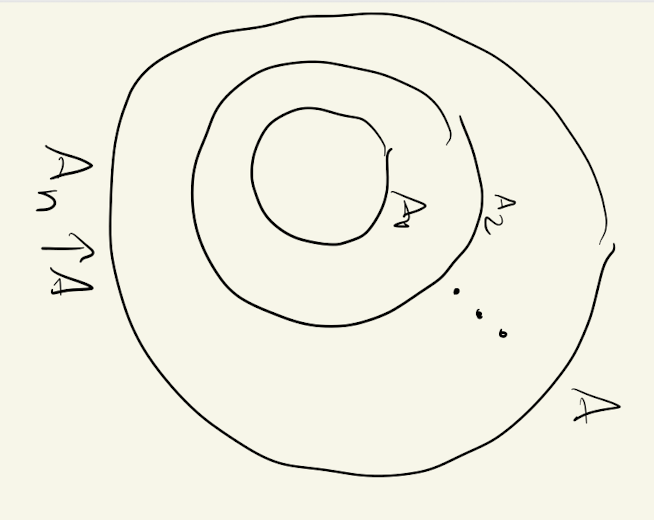
\includegraphics[width=.2\textwidth, angle=90]{images/increasing_sequence_of_sets}	
 \end{figure}
   
\item (continuity from above)  If $A_1, A_2, ... \in \F$, $A_n \downarrow A$, and $\signedmu(A_1)$ is finite, then $\signedmu(A_n) \to \signedmu(A)$ as $n \to \infty$. 
\end{alphabate}
\label{thm:continuity_of_countably_additive_set_functions}
\end{theorem}

\begin{proof}
We prove continuity from below, and leave continuity from above as an exercise to the reader (or see text). 
 
First let us assume that all $\signedmu(A_n)$ are finite (*). Then 
\ifActive 
 \textbf{Workshop Exercise}: Give the proof under this assumption. 
\vspace{2in}

\else 
\begin{align*}
A &= A_1 \cupdot (A_2 - A_1) \cupdot (A_3 - A_2) \cupdot ... && 	\text{ by } \eqref{eqn:union_as_disjoint_union_for_increasing_sequences} \\
\implies \signedmu(A) &= \signedmu(A_1) + \signedmu(A_2 - A_1) + \signedmu(A_3 - A_2) + ... && \text{(countable additivity)}\\ 
&= \signedmu(A_1) + \signedmu(A_2) - \signedmu(A_1) + \signedmu(A_3) - \signedmu(A_2) + ... && \text{(Theorem \ref{thm:basic_properties_of_finitely_additive_set_functions} \ref{itm:piece-and-difference}, (*) }\\
&= \ds\lim_{n \to \infty} \signedmu(A_n) && \text{(telescoping difference)}
\end{align*}

Now suppose $\signedmu(A_n) = \infty$ for some $n$.   So write 
\begin{align*}
A &= A_n \cupdot A- A_n && \text{(increasing sequence)}\\ 
\implies \signedmu(A) &= \signedmu(A_n) + \signedmu(A - A_n) && \text{(countable additivity)}\\  
&= \infty + \signedmu(A - A_n) 
\end{align*}

So $\signedmu(A)=\infty$.\footnote{Note that we cannot have $\signedmu(A - A_n)=-\infty$, because that would violate additivity.} Replace $A$ by $A_k$ for any $k \geq n$ to also find $\signedmu(A_k)=\infty$ for all $k \geq n$ and the result follows.

Finally suppose $\signedmu(A_n) = -\infty$ for some $n$. Then the result follows in the same way as for $\signedmu(A_n) = \infty$. 
\fi 

\end{proof}

\begin{remark}
The logic of the proof of Theorem \ref{thm:continuity_of_countably_additive_set_functions} under the finiteness assumption is as follows.  First, we re-represent the union as a disjoint union (the form is particularly simple since the sets are increasing).  This allows us to apply countable additivity. Then we apply the piece-and-difference decomposition (and the subtraction is defined under the finiteness assumption). 	
\end{remark}



\begin{remark}

In proving Theorem \ref{thm:continuity_of_countably_additive_set_functions}  for the case where $\mu(A_n) = \infty$ for some $n$, it is tempting to make the simpler argument 
\begin{align*}
\mu(A) & \geq \mu(A_n) && \text{(monotonicity)}\\	
\mu(A_k) & \geq \mu(A_n) && \text{(monotonicity)}	 
\end{align*}
for $k \geq n$.  But recall from Theorem \ref{thm:basic_properties_of_finitely_additive_set_functions} that monotonicity only holds under non-negativity, and the theorem statement is more general, applying to \textit{signed} set functions as well. 
\end{remark}

\begin{remark}
Theorem \ref{thm:continuity_of_countably_additive_set_functions} still holds if $\F$ is only assumed to be a field, so long as the limit sets $A$ belong to $\F$.  %We will use this formulation later when we want to extend the set function $\mu(a,b]=b-a$ from a field (of disjoint unions of right semi-closed intervals) to a sigma field. 
\end{remark}

We have the result that finite additivity plus continuity equals countable additivity. 

\begin{theorem}
Let $\fasf$ be a finitely additive set function on the field $\F_0$.  Suppose either
\begin{alphabate}
\item $\fasf$ is continuous from below
\item $\fasf$ is continuous from above at the empty set.	
\end{alphabate}
Then $\fasf$ is countably additive.
\label{thm:finite_additivity_plus_continuity_gives_countable_additivity}
\end{theorem}

\begin{proof}
We prove that the conclusion holds under (a) and leave doing the same for (b) as an exercise to the reader (or see text). 	%To show that $\fasf$ is countably additive, we need to show that  $ \fasf \bigg( \bigcupdot_{n=1}^\infty A_n \bigg) = \ds\sum_{n=1}^\infty \fasf(A_n)$.   

Given $A = \bigcupdot_{n=1}^\infty A_n$, we define $P_n := \bigcup_{m \leq n} A_n$ and so $P_n \uparrow A$.   So we have
\begin{align*}
\fasf(P_n) &\to \fasf(A) && \text{(continuity from below)} \\
\implies \fasf(\bigcup_{m \leq n} A_n) &\to \fasf(A) && \text{(definition)} \\	
\implies \ds\sum_{m=1}^n \fasf(A_n) &\to \fasf(A) && \text{(finite additivity)} \\
\end{align*}
Taking $n \to \infty$ gives countable additivity.
\end{proof}


\subsection{Borel-Cantelli Lemma}

\begin{lemma}{\textbf{Borel Cantelli Lemma}}
If $A_1, A_2, ... \in \F$ and $\sum_{n=1}^\infty \mu(A_n) < \infty$, then $\mu(\limsup_{n \to \infty} A_n) = 0$.
\label{lemma:borel_cantelli}
\end{lemma}

\begin{proof}\footnote{\cite{ash2000probability} has a proof that does not require continuity of measure, although I currently personally enjoy its role here.}
Recall from Definition \ref{def:upper_limit} that
\[ \explaintermbrace{$:=B$}{\limsup_{n \to \infty} A_n} = \bigcap_{k=1}^\infty \explaintermbrace{$:=B_k$}{\bigcup_{n=k}^\infty A_n} = \set{x : x \in A_n \text{ i.o. }}  \]	
where we have also introduced some notation for convenience.

Now $B_{k+1} \subset B_k$ and $\cap_{k=1}^\infty B_k =B$, so $B_k \downarrow B$.  Since also $\mu(B_1) < \infty$ (by hypothesis and monotonicity), then we can apply continuity from above (Theorem~\ref{thm:continuity_of_countably_additive_set_functions}) to get
\begin{align*}
\mu(B) &= \ds\lim_{k \to \infty} \mu(B_k) \\
&= 	\ds\lim_{k \to \infty} \mu \bigg( \bigcup_{n=k}^\infty A_n \bigg) && \tinytext{def. $B_k$} \\
&\leq \ds\lim_{k \to \infty} \ds\sum_{n=k}^\infty \mu (A_n) && \tinytext{subadditivity} \\
&=0 && \tinytext{convergent series have vanishing tails}
\end{align*}
  
\end{proof}

\begin{remark}{\remarktitle{Intuition for Borel-Cantelli}}
An attempt at a verbal description of the proof of Lemma \ref{lemma:borel_cantelli} follows:  Convergent series of real numbers have arbitrarily small tails. When the series is constructed of measures $(\sum_{n=1}^\infty \mu(A_n))$, this implies that the measure of the tail $(\cup_{n=k}^\infty A_n)$ is arbitrarily small (by subadditivity).  Now $\limsup_{n \to \infty} A_n$ is the set of points in $\set{A_n}$ i.o., so such points must be in \textit{all} tails $(\cap_{k=1}^\infty \cup_{n=k}^\infty A_n)$, and by continuity of measure (from above), the measure of such a set is the limit of the measure of the tail, i.e. 0.
\end{remark}

	


%By , we have


 %we break up the limit of the increasing sequence into a disjoint union as follows	



 \section{$\S$ 1.3: Extension of measures} \label{sec:extension_of_measures}
 
 
\subsection{Extension and approximation} \label{sec:extension_and_approximation}
 
In Example \ref{ex:Lebesgue_measure}, we discussed the concept of length of a subset of $\R$; in particular, we mentioned extending the set function given on intervals by $\mu(a,b] = b-a$ to a larger class of subsets of $\R$.  


 As remarked in Example \ref{ex:field_of_finite_disjoint_unions_of_rsc_intervals}, if we define $\F_0 = \set{\text{finite disjoint unions of right semi-closed intervals } (a,b], a < b}$, then $\F_0$ is a field, as can be easily verified.  And $\mu$ can easily be extended to be a finitely additive set function on $\F_0$.   

\begin{figure}[H]
\centering
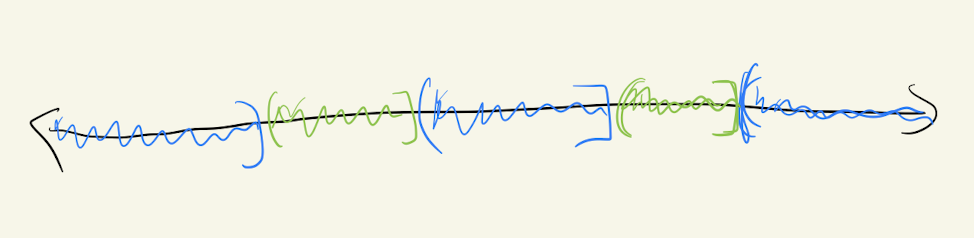
\includegraphics[width=.6\textwidth]{images/rsc_intervals}	
\end{figure}

However, $\F_0$ is not a $\sigma$-field.   So how can we extend this function to a measure on a larger class of subsets?  For instance, we would at least like to be able to measure intervals such as $(a,b), [a,b)$ or $[a,b]$ and points $\set{x}$.   The challenges are:

\begin{itemize}
\item \textit{We need to show that $\mu$ is countably additive.} We will do this in Section ?.   Moreover, in that section, we will generalize our problem to set functions given by $\mu(a,b] = F(b)-F(a)$, where $F$ is an increasing right-continuous function from $\R$ to $\R$.
\item \textit{We need to extend $\mu$ to $\sigma(\F_0)$, the minimal $\sigma$-field containing $\F_0$.} In other words, we need to extend $\mu$ to the Borel sets.  We will handle the problem in this section more generally.  In this section, we will deal with the problem of extending a measure on $\F_0$ to a measure on $\sigma(\F_0)$. We do so using \Caratheodory's Theorem  (Theorem \ref{thm:caratheodory_extension}).  Along the way, we will use Theorem \ref{thm:extension_of_finite_measure} and Theorem \ref{thm:monotone_class_theorem} to prove Theorem \ref{thm:caratheodory_extension}. 
% We refer to a countably additive set function $\mu$ on a field $\F_0$ as a \textit{pre-measure}
\end{itemize}

 \begin{theorem}
 (Theorem 1.3.6 \cite{ash2000probability}) A finite measure on a field $\F_0$ can be extended to a measure on $\sigma(\F_0)$. 	
 \label{thm:extension_of_finite_measure}
 \end{theorem}

\begin{proof}
See pp. 12-17 of \cite{ash2000probability}.	
\end{proof}

\begin{theorem}{\textbf{(Monotone Class Theorem)}}
Let $\F_0$ be a field of subsets of $\Omega$ and $\C$ be a class of subsets of $\Omega$ that is monotone (if $A_n \in \C$ and $A_n \uparrow 
A$ or $A_n \downarrow A$, then $A \in \C$).  If $\C \supset \F_0$ then $\C \supset \sigma(\F_0)$, then minimal $\sigma$-field over $\F_0$. 
 \label{thm:monotone_class_theorem}
\end{theorem}

\begin{proof}
See pp. 18-19 of \cite{ash2000probability}.	
\end{proof}

\begin{remark}
During the proof of Theorem \ref{thm:monotone_class_theorem}, some key observations are made about the relationship between monotone classes and $\sigma$-fields:
\begin{alphabate}
\item A monotone class that is also field is a sigma-field.  (See Remark \ref{rk:the_limits_of_increasing_and_decreasing_sequences_of_sets_in_a_field_are_also_the_countable_unions}.)
\item The smallest monotone class and smallest sigma-field over a field coincide. 
\end{alphabate}
\label{rk:monotone_classes_and_sigma_fields}
\end{remark}

\begin{remark}{\remarktitle{The utility of the Monotone Class Theorem}}
The Monotone Class Theorem provides an alternate route towards executing on the Good Sets Strategy (Section \ref{sec:good_sets_strategy}.)  Suppose you want to show that all members of a $\sigma$-algebra   $\F$ have some property $P$.  Define ``good sets" as those that satisfy the property
\[ \G := \{ G \in \F : G \text{ has property } P \} \]
The strategy is then to simply
\begin{enumerate}
\item Show $\G$ contains some class $\C$ such that $\F = \sigma(\C)$
\item Show $\G$ is a monotone class.  
\end{enumerate}	 
\label{rk:monotone_class_theorem_for_executing_good_sets_strategy}
\end{remark}

\begin{remark}
The strategy in Remark \ref{rk:monotone_class_theorem_for_executing_good_sets_strategy} is very much like induction.  Step \#1 is the ``base" step and step \#2 is the ``induction" step.
\end{remark}

For an example of where the strategy in Remark \ref{rk:monotone_class_theorem_for_executing_good_sets_strategy} is used, see the proof of uniqueness in the \Caratheodory~Extension Theorem (Theorem \ref{thm:caratheodory_extension}).  It is also used extensively to show that Borel sets have some property; see Section \ref{sec:properties_of_borel_sets}.


\begin{theorem}{\textbf{(\Caratheodory~Extension Theorem)}} Let $\mu$ be a pre-measure on a field $\F_0$ of subsets of $\Omega$, and assume that $\mu$ is $\sigma$-finite on $\F_0$, so that $\Omega$ can be decomposed as $\cup_{n=1}^\infty A_n$ where $A_n \in \F_0$ and $\mu(A_n) < \infty$ for all $n$.  Then $\mu$ has a unique extension to a measure on $\F := \sigma(\F_0)$, the minimal $\sigma$-field over $\F_0$. 
 \label{thm:caratheodory_extension}
\end{theorem}

\begin{proof} (We follow the argument of \cite{ash2000probability}, but add some detail.) 
First we prove existence.  {\footnotesize [Without loss of generality, we assume the $A_n$ are disjoint.  This is possible because we can use \eqref{eqn:union_as_disjoint_union} to re-express the countable union as a disjoint countable union:  $\Omega = \cup_{i=1}^\infty A_i = \cupdot_{i=1}^\infty B_i$, where $B_i := A_i \cap A_{i-1}^c ... \cap A_1^c$.]  } 

If we define $\mu_n(A)=\mu(A \cap A_n)$ for each $A \in \F_0$, then we can decompose $\mu$ into a countable sum of finite measures:
\begin{itemize}
\item $\mu_n$ is a measure on $\F_0$. {\footnotesize   [Its countable additivity is inherited from $\mu$. If $\cupdot_{i=1}^\infty A_i$ is a disjoint union, then so is $\cupdot_{i=1}^\infty (A_i \cap A_n)$, and $\mu( \cupdot_{i=1}^\infty (A_i \cap A_n)) = \sum_{i=1}^\infty \mu(A_i \cap A_n) $ since $A_i \cap A_n$ are in $\F_0$. ] }
\item $\mu_n$ is finite.  {\footnotesize  [True because $\mu_n(A) = \mu(A \cap A_n) \stackrel{\text{monotonicity}}{\leq} \mu(A_n) < \infty$.]	 }
\item  $\mu = \sum_{n=1}^\infty \mu_n$. {\footnotesize  [True because $\mu(A) = \mu(A \cap \Omega) = \mu(A \cap (\cupdot_{n=1}^\infty A_n)) =\mu(\cupdot_{n=1}^\infty (A \cap A_n)) = \sum_{n=1}^\infty \mu(A \cap A_n) = \mu_n (A). $] }
\end{itemize}
Now by Theorem \ref{thm:extension_of_finite_measure}, we can extend each $\mu_n$ to a measure $\mu_n^*$ on $\F$.   Thus $\mu^* := \sum_{n=1}^\infty \mu_n^*$ extends $\mu$ to $\F$.  Moreover, $\mu^*$ is still a measure since the order of summation in a double series of nonnegative terms can be reversed.  {\footnotesize   [Countable additivity still holds  since:

\begin{align*}
\mu^*(\cupdot_{i=1}^\infty A_i) &= \ds\sum_{n=1}^\infty \mu_n^* (\cupdot_{i=1}^\infty A_i) && \\ &= \ds\sum_{n=1}^\infty \ds\sum_{i=1}^\infty \mu_n^* (A_i) && \tinytext{$\mu_n^*$ is measure, so countably additive}\\
	&= \ds\sum_{i=1}^\infty \ds\sum_{n=1}^\infty \mu_n^*(A_i) && \tinytext{reverse order of summation for double series with non-negative terms} \\
	&= \ds\sum_{i=1}^\infty \mu^*(A_i) && \tinytext{def. of $\mu^*$}
\end{align*}

]. }


Now we prove uniqueness.   That is, we prove that if $\lambda$ is a measure on $\F$ and $\lambda = \mu^*$ on $\F_0$, then $\lambda = \mu^*$ on $\F$.    To see this, as before, we decompose the measure into a sum of finite measures: $\lambda = \sum_{n=1}^\infty \lambda_n$ where $\lambda_n := \lambda (A_n \cap A)$.  Now by assumption $\lambda_n = \mu_n^*$ on $\F_0$.  Where are they equal on $\F$?  Let us define the ``good sets" (recall Section \ref{sec:good_sets_strategy})
\[ \G : = \set{A \in \F : \lambda_n (A) = \mu_n^* (A)} \]
Now we can show $\G = \F$ -- that is, \textit{all} sets in the $\sigma$-field are good sets -- by observing
\begin{itemize} 
\item 	 $\G$ is a monotone class.  {\footnotesize 
[This is true by continuity from below (see Theorem \ref{thm:continuity_of_countably_additive_set_functions}). In particular, a countable union can be considered the limit of an increasing sequence of partial unions (See Remark \ref{rk:the_limits_of_increasing_and_decreasing_sequences_of_sets_in_a_field_are_also_the_countable_unions}.) As a result, the measure of the limiting set is determined, as the limit of the the measure of the sets in that sequence.] }
\item $\G \supset \F_0$. {\footnotesize 
[This is true by construction.] }
\end{itemize} 
And so by Monotone Class Theorem (Theorem \ref{thm:monotone_class_theorem}), we have $\G \supset \F$.  But by construction $\G \subset \F$, and so $\G = \F$.  Therefore $\lambda_n = \mu_n^*$ for each $n$.  

So 
\[ \lambda \stackrel{\text{decomposition}}{=} \sum_n \lambda_n = \sum_n \mu_n^* \stackrel{\text{recomposition}}{=} \mu^*, \] proving uniqueness.
\end{proof}


\begin{remark}{\remarktitle{Folland's statement of \Caratheodory's extension theorem, with explicit construction of the measure.}}
\cite[Thm.~1.14]{folland1999real} gives a useful version of Theorem \ref{thm:caratheodory_extension},  which provides an explicit construction of the measure extended from a pre-measure. {\tiny (The constructiveness will be useful e.g. for product measures (see Sec.~\ref{sec:product_measure}; in particular see the product measure of the unit square diagonal under lebesgue and counting measure factors Ex.~\ref{ex:lebesgue_counting_measure_on_the_unit_square_diagonal}.)}

Folland's construction is as follows:  Let $\F_0 \subset \mathcal{P}(\Omega)$ be a field, $\mu_0$ be a premeasure on $\F_0$, and $\F = \sigma(\F_0)$.   Then there exists a measure $\mu$ on $\F$ such that $\mu |_{\F_0} = \mu_0$, namely
for all $A \in \F$,
%
\begin{align}
\mu(A) = \inf \bigg\{ \ds\sum_{j=1}^\infty \mu_0(A) : A_j \in \F_0, \bigcup_{j=1}^\infty A_j \supset A  \bigg\} 
\label{eqn:explicit_construction_of_measure_extended_from_premeasure}	
\end{align}
%
Folland's construction also highlights that the $\sigma$-finite assumption in Theorem \ref{thm:caratheodory_extension} is only necessary for uniqueness. 
\end{remark}

\begin{remark}{\remarktitle{Folland's statement of \Caratheodory's extension theorem does not require $\sigma$-finite pre-measures.}}
In \cite[Thm.~1.14]{folland1999real}, we see that the extension theorem also applies to non-$\sigma$-finite pre-measures, but in that case, we lose uniqueness.
\label{rk:extension_theorem_gives_uniqueness_iff_the_premeasure_is_sigma_finite} 
\end{remark}

\begin{remark}
The proof of Theorem \ref{thm:caratheodory_extension} reveals the appeal of $\sigma$-finite measures -- they can be decomposed as the countable sum of finite measures (and the order of summation of double series can be reversed for nonnegative series, so countable additivity still holds). 
\end{remark}




In Remark \ref{rk:monotone_classes_and_sigma_fields} (b), we observed that minimal $\sigma$-fields over a field can be characterized as the minimal monotone classes over a field -- so we merely need to close the field over increasing and decreasing sequences of sets.   This idea suggests that if $\F_0$ is a field and $\F = \sigma(\F_0)$, sets in $\F$ can be approximated in some sense by sets in $\F_0$.  The following result formalizes this notion. 


\begin{theorem}{\textbf{(Approximation Theorem)}} Let $(\Omega, \F, \mu)$ be a measure space.  Let $\F = \sigma(\F_0)$ where $\F_0$ is a field of subsets of $\Omega$.  Let $\mu$ be $\sigma$-finite on $\F_0$.  Then for every $A \in \F$ and fixed $\epsilon >0$, there is a set $B \in \F_0$ such that $\mu( A \triangle B) < \epsilon$.  
\label{thm:approximation theorem}	
\end{theorem}


\begin{example}

This interesting example (from \cite{ash2000probability} pp. 20) provides a counterexample to the theorems when $\F_0$ is not $\sigma$-finite. 

\begin{figure}[h!]
\centering
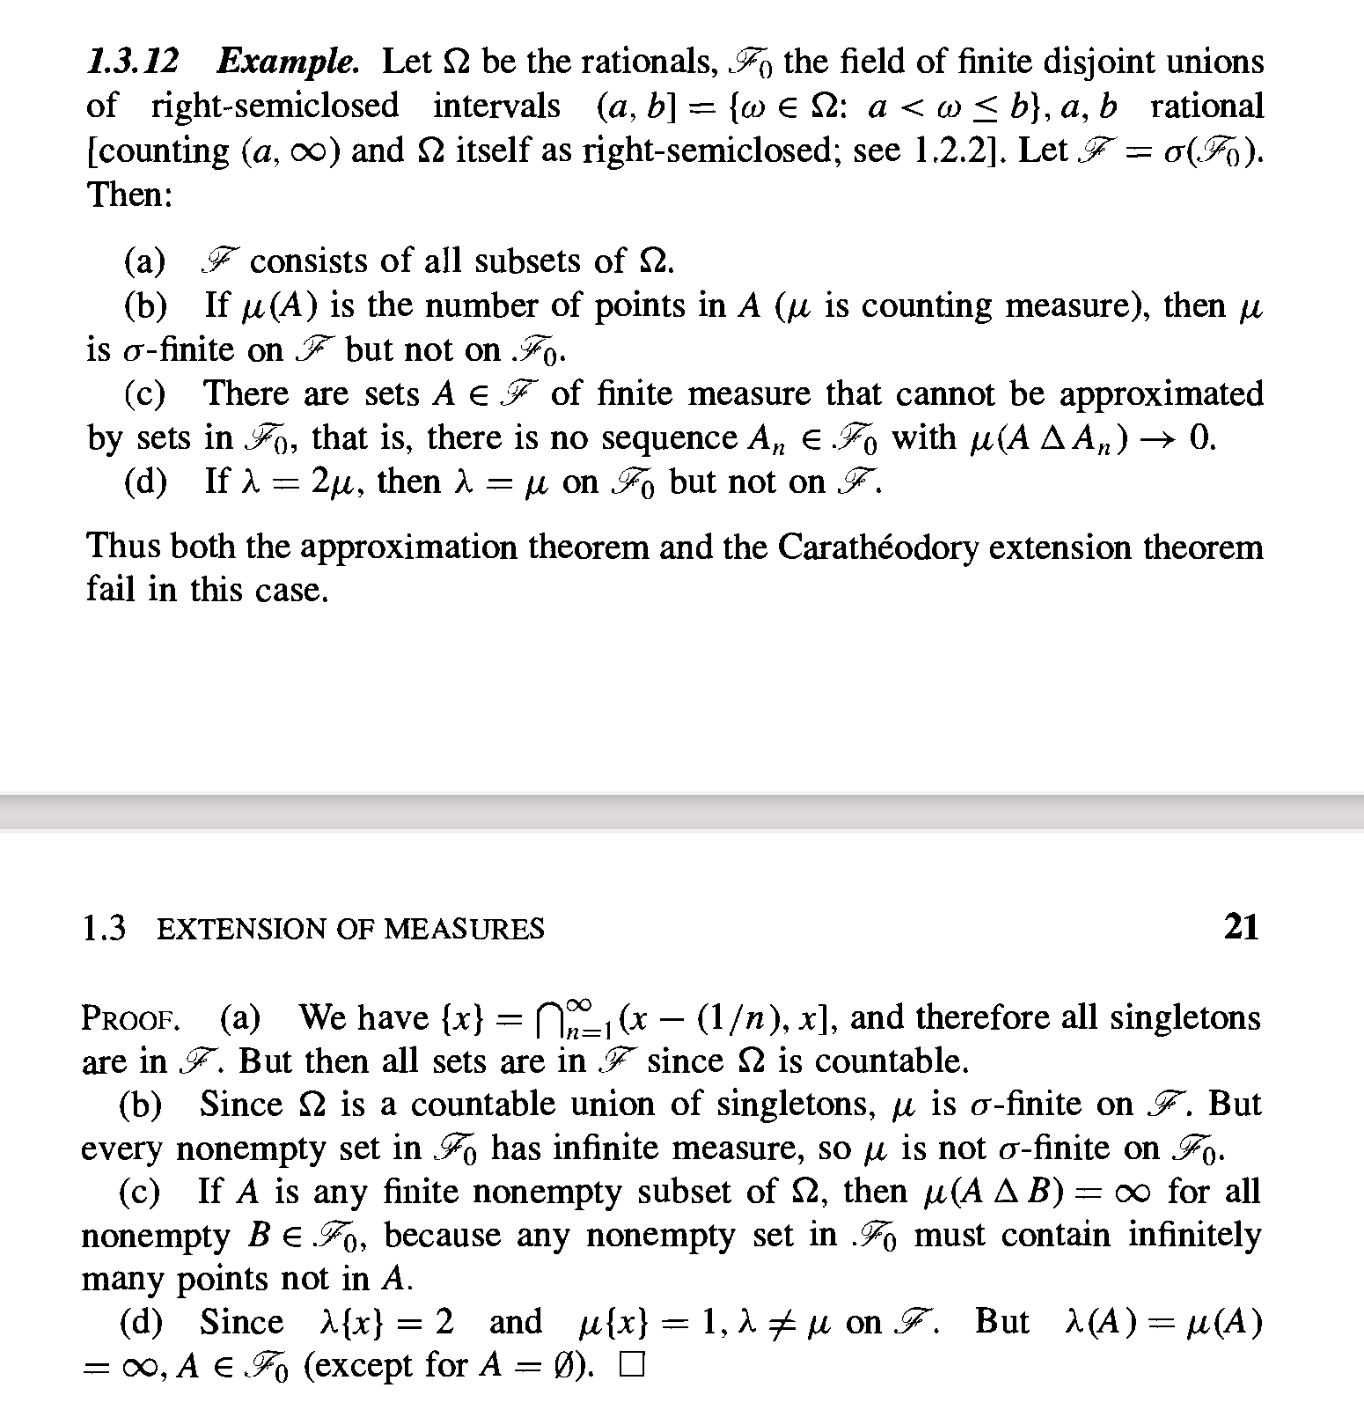
\includegraphics[width=1.\textwidth]{images/example_of_extension}	
\end{figure}
\end{example}

\subsection{Completion of measure spaces} \label{sec:completion_of_measure_spaces}

\begin{definition}
A measure $\mu$ on a $\sigma$-field $\F$ is said to be \textit{complete} iff whenever $A \in F$ and $\mu(A) =0$, we have $B \in F$ for all $B \subset A$.
\end{definition}

\begin{definition}
The \textit{completion} of a measure space $(\Omega, \F, \mu)$ is given by $(\Omega, \F_\mu, \mu)$, where 
\[ \F_\mu := \set{A \cup S : A \in \F, S \subset N 
\text{ for some } N \in \F \text { with } \mu(N) = 0 } \]
and where $\mu$ is extended to $\F_\mu$ by setting $\mu (A \cup S) = \mu(A)$.
\label{def:completion_of_measure_space}
\end{definition}

\begin{remark}
Let us show that Definition \ref{def:completion_of_measure_space} is a valid definition by showing that

\begin{enumerate}
\item \textit{$\F_\mu$ is a $\sigma$-field.}
\item \textit{$\mu$ is a measure on $\F_\mu$.}
\item \textit{The completion is complete.} 	
\end{enumerate}

We justify these in turn:

\begin{enumerate}
\item $\F_\mu$ is closed under countable unions, since 
\[ \cup_{i=1}^\infty (A_i \cup S_i) =  \explaintermbrace{$\in \F$}{(\cup_{i=1}^\infty A_i)} \; \cup \; \explaintermbrace{has measure 0}{(\cup_{i=1}^\infty S_i)} \]
 where the term on the right has measure 0 because $\cup_{i=1}^\infty S_i \subset \cup_{i=1}^\infty N_i \in \F$, and $\mu(\cup_{i=1}^\infty N_i) = \sum_{i=1}^\infty \mu(N_i)= 0$.
 
 $F_\mu$ is also closed under complements, since $S \subset N \implies N^c \subset S^c$, and so
 \[ ( A \cup S)^c = (A^c \cap S^c) = \explaintermbrace{$\in \F$}{(A^c \cap N^c)} \cup \explaintermbrace{has measure 0}{(A^c \cap S^c - N^c)} \]
 where the term on the right has measure 0 by monotonicity, because $A^c \cap S^c - N^c \subset S^c - N^c = S^c \cap (M^c)^c = S^c \cap N \subset N$.
\item First, we show that countable additivity holds in $\F_\mu$. 
\[ \mu(\cupdot_{i=1}^\infty  (A_i \cup S_i)) \stackexplain{see below}{=} \mu(\cupdot_{i=1}^\infty A_i) \stackexplain{$\mu$ countably additive on $\F$ \; }{=} \sum_{i=1}^\infty \mu(A_i) \stackexplain{construction of extension}{=}  \sum_{i=1}^\infty \mu(A_i \cup S_i)  \]
The first equality holds because we can re-represent a disjoint union  $\cupdot_{i=1}^\infty  (A_i \cup S_i) = (\cupdot_{i=1}^\infty A_i) \cup (\cupdot_{i=1}^\infty S_i) $.  Since $\cupdot_{i=1}^\infty S_i  \subset \explaintermbrace{has measure 0 in $\F$}{\cupdot_{i=1}^\infty N_i}$, we have that $\mu((\cupdot_{i=1}^\infty A_i) \cup (\cupdot_{i=1}^\infty S_i)) = \mu(\cupdot_{i=1}^\infty A_i)$. 

Next, we show that $\mu$ is invariant to decompositions: if $A_1 \cup S_1 = A_2 \cup S_2$, then $\mu(A_1 \cup S_1) = \mu(A_2 \cup S_2)$, or more simply $\mu(A_1)=\mu(A_2)$.

\begin{figure}[H]
\centering
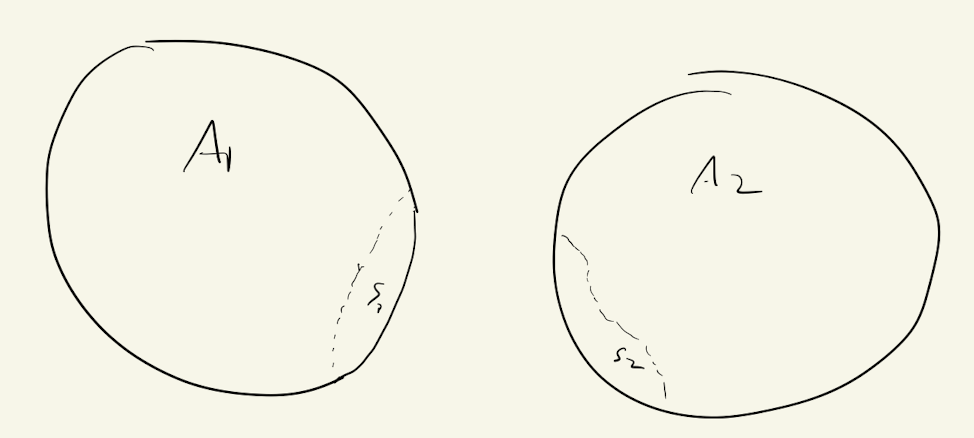
\includegraphics[width=.4\textwidth]{images/completion_of_measure_space}	
\end{figure}

We have    
\[ \mu(A_1)  \stackexplain{countable additivity}{=} \mu(A_1 \cap A_2) + \mu(A_1 \cap A_2^c)\stackexplain{see below}{=} \mu(A_1 \cap A_2) \stackexplain{monotonicity}{\leq} \mu(A_2) \]
where the second equality holds since $A_1 \cap A_2^c \subset S_2$ {\footnotesize (which, in turn, holds since $x \in A_1 \implies x \in A_2 \text{ or } x \in S_2$, so $x \in A_1 \text{ and } x \not\in A_2 \implies x \in S_2$)} .

By symmetry, $\mu(A_2) \leq \mu(A_1)$, so $\mu(A_1)=\mu(A_2)$. 
\item By the definition of a complete measure, we need to show that if $B \in \F_\mu$ and $\mu(B)=0$ then $C \in \F_\mu$ for all $C \subset B$.

%Now $B \in \F_\mu \implies B = \explaintermbrace{$\in \F$}{A} \cup \explaintermbrace{has measure 0}{S}$.  

Now $B \in \F_\mu \implies B = \explaintermbrace{$\in \F$}{A} \cup \explaintermbrace{$\subset N \in \F : \mu(N)=0$}{S}$.  

So our assumption $\mu(B) = 0$ gives us $\mu(A) = 0$, since $\mu(B) = \mu(A \cup S) \stackrel{\text{choice of extension}}{=} \mu(A)  =0$.

Now since we have assumed $C \subset B$ we have
\[\mu(C) \stackexplain{monotonicity}{\leq} \mu(B) \stackrel{B \in \F_\mu}{=} \mu(A \cup S)  \stackexplain{subadditivity}{\leq} \mu(A)+\mu(S)  \stackexplain{see above}{=} 0 + \mu(S) = 0 + 0= 0\]

Since $\mu$ is non-negative, this implies that $\mu(C) =0$.  

We can therefore write $C = \explaintermbrace{$\in \F$}{\emptyset} \cup \explaintermbrace{has measure 0}{C}$, so $C \in \F_\mu$.

Thus, $\mu$ on $\F_\mu$ is complete, since any subset of measure 0 is contained in $\F_\mu$.  
\end{enumerate}
\label{rk:completion_of_measure_space_is_well_defined} 
\end{remark}


\begin{example}
Let us provide a simple example of where completing a measure space generates new measurable sets. Consider a measure space given by $(\Omega, \F, \mu)$ where $\Omega=\R$, $\F = \set{\emptyset, A, A^c, \Omega}$ where we take $A=[0,1]$ for concreteness, and where $\mu$ is defined by $\mu(A^c)=1$ and $\mu(A)=0$.  The measure space is not complete, since no proper subset of $A$  is contained in $\F$. (For example, $[0,\half] \not\in \F$.)  If we complete the measure space, we obtain $(\Omega, \F_\mu, \mu)$ where $\F_\mu = \set{\emptyset, A, A^c, \Omega, \text{ any subset of } [0,1]}$.
\end{example}

\begin{problem}
Let $(\Omega, \F, \mu)$ be a complete measure space.  If $f: (\Omega, \F) \to (\Omega', \F')$ and $g: \Omega \to \Omega'$, $g=f$ except on a subset of a set $A \in \F$ with $\mu(A)=0$, show that $g$ is measurable (relative to $\F$ and $\F'$)
\label{prob:in_a_complete_metric_space_you_are_a_measurable_function_if_you_are_equal_to_some_other_measurable_function_ae}
\end{problem}

\begin{proof}[Solution.]
For all $A \in \F'$, 
{\footnotesize 
\begin{align*}
g^{-1}(A) &= \biggset{x: x \in g^{-1}(A) \text{ and } x \in f^{-1}(A)} && \bigcup \biggset{x: x \in g^{-1}(A) \text{ and } x \not\in f^{-1}(A)}	 \\
&= \explaintermbrace{$\in \F$ since $f$ measurable}{\set{x \in f^{-1}(A)}}\setminus \explaintermbrace{$\in \F$ by completeness, as a subset of a set of measure 0 }{\biggset{x : x \in f^{-1}(A) \text{ and } x \not\in g^{-1}(A)}} && \bigcup \explaintermbrace{$\in \F$ by completeness, as a subset of a set of measure 0 }{\biggset{x: x \in g^{-1}(A) \text{ and } x \not\in f^{-1}(A)}}
\end{align*}
 }
 
So by closure properties of $\sigma$-fields, $g^{-1}(A) \in \F$. 

 \begin{figure}[H]
 \centering
 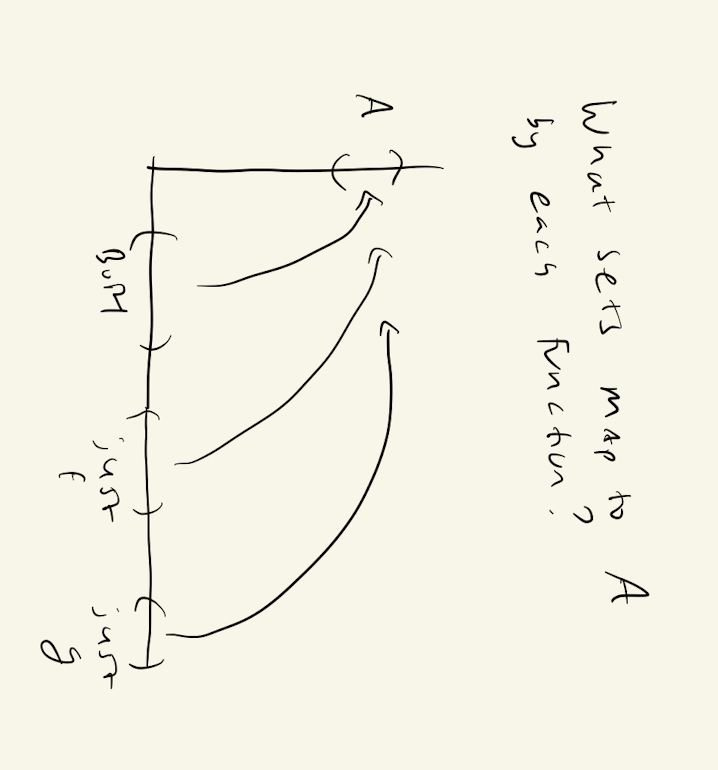
\includegraphics[width=.4\textwidth, angle=90]{images/measurability_of_functions_in_complete_measure_spaces_from_ae_equality}
 \end{figure}

\end{proof}



 \section{$\S$ 1.4: Lebesgue-Stieltjes Measures and Distribution Functions} \label{sec:ls_measures_and_distribution_functions}
 
 \begin{definition}
 A \textit{Lebesgue-Stieltjes measure} on $\R$ is a measure $\mu$ on $\B(\R)$ such that $\mu(I) < \infty$ for each bounded interval $I$.	
 \end{definition}

\begin{definition}
 A \textit{distribution function} on $\R$ is a map $F : \R \to \R$ that is increasing [ $a<b$ implies $F(a) \leq F(b)$] and right continuous [ $\lim_{x \downarrow x_0} F(x) = F(x_0)$]. 
 \end{definition}
 

In this Section, we show that the formula $\mu(a,b] = F(b) - F(a)$ sets up a one-to-one correspondence between distribution functions and Lebesgue-Stieltjes measures.  {\tiny (For reference, Fig.~\ref{fig:distribution_function_with_positive_mass_on_points_that_is_not_concentrated_on_a_countable_set} shows a distribution function.)}
 
 \subsection{$\S$ 1.4.2 Each Lebesgue-Stietljes measure uniquely determines a distribution function (up to an additive constant)}
 First, the easy part: we show that to every Lebesgue-Stieltjes  measure, there is a unique distribution function (up to an additive constant). 
 
 \begin{theorem}
 Let $\mu$ be a Lebesgue-Stietljes measure on $\R$.  Let $F : \R \to \R$ be defined (up to additive constant) by $F(b)-F(a) = \mu(a,b]$ for $a<b$. Then $F$ is a distribution function.
\label{thm:from_ls_measure_to_distribution_function}
 \end{theorem}

\begin{proof}
We must show that $F$ is increasing and right continuous.

\ifActive 
\textbf{Workshop Exercise}: Finish the proof.
\else 
\begin{enumerate}
\item We have $F(b) - F(a) = \mu(a,b] \geq 0$, since $\mu$ is non-negative. So $F$ is increasing.  
\item By the continuity (from above) of measure (which can be applied since since Lebesgue-Stietljes measures are finite on any interval), 
\[ \ds\lim_{b' \downarrow b}[F(b') - F(a)] = \ds\lim_{b' \downarrow b} \mu(a,b'] = \mu(a,b]\]

Thus, rearranging,
\[ \ds\lim_{b' \downarrow b} F(b') = \mu(a,b] + F(a) = \bigg(F(b)-F(a)\bigg) + F(a) = F(b)\]
So $F$ is right continuous.  
\end{enumerate}
\fi 
\end{proof}


  \subsection{$\S$ 1.4.3-1.4.4 Each distribution function (identified up to additive constant) uniquely determines a Lebesgue-Stietljes measure }
  
 Now the harder part.  We need to show that every distribution function $F$ (identified up to additive constant) uniquely determines a Lebesgue-Stieltjes  measure.  
 
 We will temporarily work with $\overline{\R}$, because it is a compact space, and then convert back to $\R$.  In $\overline{\R}$, by a similar reasoning as we've seen before (e.g. see Section \ref{sec:extension_and_approximation}), it is straightforward to show that the formula $\mu(a,b] = F(a)-F(b), a,b \in \overline{\R}, a <b$ defines a finitely additive set function on $\F_0(\overline{\R})$, the field of disjoint unions of right semi-closed intervals of the extended reals.  
 
 The challenge will be to show that this set function is countably additive.  If we can do that, then we can apply Carath\'eodory's Extension Theorem to extend the corresponding function $\mu$ on $\F_0(\R)$ to $\B(\R)$, as will be done in Theorem \ref{thm:extension_for_Lebesgue_stietljes_measure}. 

\begin{lemma}
The set function $\mu$ is countably additive on $\F_0(\overline{\R})$.
\label{lemma:ls_measures_are_countably_additive_on_the_field_of_disjoint_rsc_intervals} 	
\end{lemma}

\begin{proof}
We assume $F(\infty) - F(-\infty) < \infty$, so that $\mu$ is finite.   (We leave the case where $F(\infty) - F(-\infty) = \infty$	to the reader, or see the text.)  Our strategy will be to show that $\mu$ is continuous from above, in which case we can apply Theorem \ref{thm:finite_additivity_plus_continuity_gives_countable_additivity} (b) to show that the set function is countably additive.

Let $A_n$ be a sequence of sets in $\F_0(\overline{\R})$ such that $A_n \downarrow \emptyset$.  Now each $A_n$ is a finite union of disjoint r.s.c. intervals.

\begin{figure}[H]
\centering
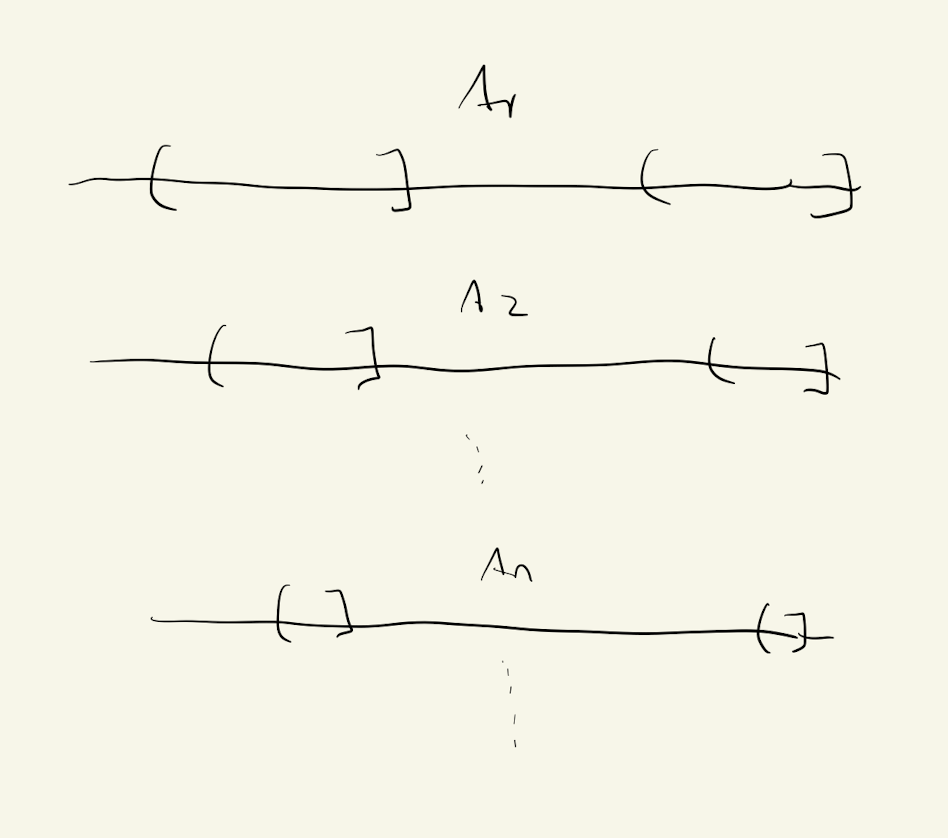
\includegraphics[width=.45\textwidth]{images/decreasing_sequence_of_union_of_rsc_intervals}	
\end{figure}

 Suppose one such interval is $(a,b]$.  By the right continuity of $F$, we can find intervals $(a',b]$ that approximate $(a,b]$ from the inside arbitrarily well, since by continuity from below
\[ \mu(a',b] = F(b) - F(a') \to \mu(a,b] = F(b) - F(a) \text{ as } a' \downarrow a \] 

\begin{figure}[H]
\centering
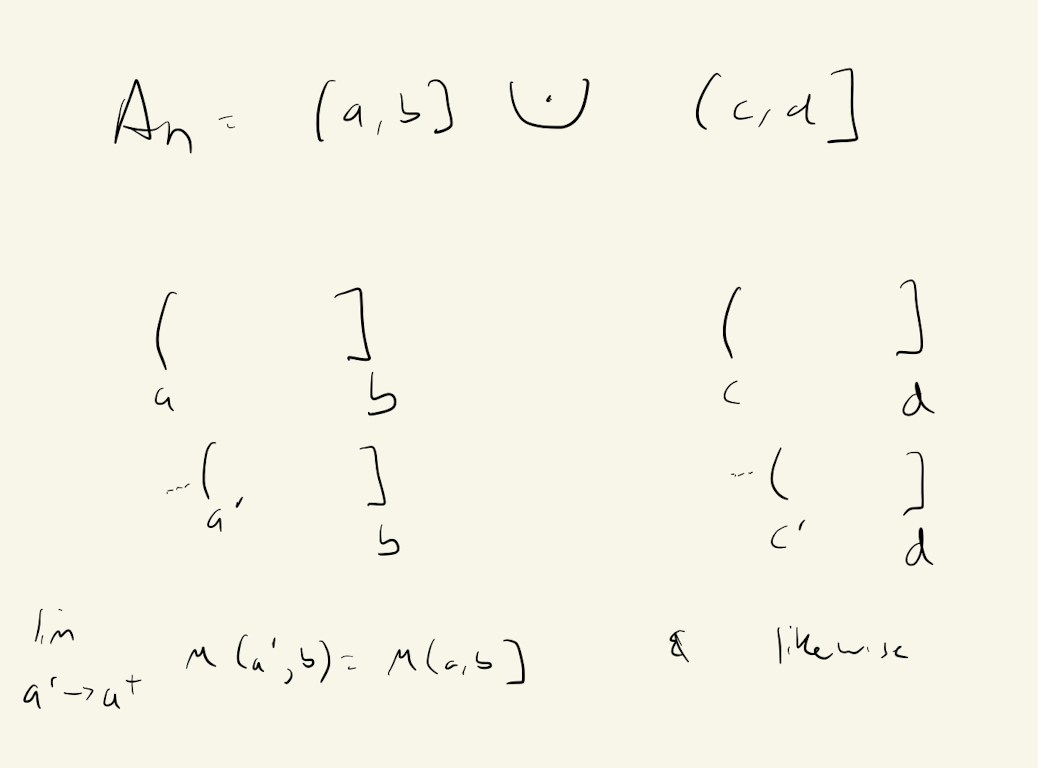
\includegraphics[width=.45\textwidth]{images/approximating_union_of_rsc_intervals}	
\end{figure}

Thus, we can find sets $B_n \in \F_0(\overline{\R})$  where $\mu(B_n)$ approximates $\mu(A_n)$ to any desired $\epsilon > 0$ that satisfy $B_n \subset \overline{B}_n \subset A_n$.  By these inclusion properties and the decreasing nature of the sequence, we have:
\begin{alphabate}
\item $\cap_{n=1}^\infty \overline{B}_n = \emptyset$.	\quad  {[\footnotesize True because each $\overline{B}_n \subset A_n$, so $\cap_{n=1}^\infty \overline{B}_n \subset \cap_{n=1}^\infty A_n = \emptyset$.  ]} 
\item $\cap_{k=1}^n \overline{B}_k = \emptyset$ for sufficiently large $n$.	\quad  {\footnotesize [We have $\overline{\R} \; \stackrel{ \text{item a)}}{=} \; (\overline{\R} - \cap_{n=1}^\infty \overline{B}_n) \; \stackrel{\text{DeMorgan } \eqref{eqn:demorgan_for_relative_complements}}{=} \; \cup_{n=1}^\infty (\overline{\R} - \overline{B}_n)$.   So $\set{\overline{\R} - \overline{B}_n}$ is an open cover of the compact space $\overline{\R}$. By the Heine-Borel theorem, there must be a finite subcover.  So for sufficiently large $n$, we have $\cup_{k=1}^n (\overline{\R} - \overline{B}_k) = \overline{\R}$.  Taking complements of both sides, and once again applying DeMorgan's law \eqref{eqn:demorgan_for_relative_complements} to the relative complement, we find $\cap_{k=1}^n \overline{B}_k = \emptyset$.  ]}
\item $\cap_{k=1}^n B_k = \emptyset$ for sufficiently large $n$. {\footnotesize [This follow from item b) and the fact that each $B_k \subset \overline{B}_k$.]}
\end{alphabate}

So now we use a piece-and-difference decomposition (Theorem \ref{thm:basic_properties_of_finitely_additive_set_functions} (b) ):
\begin{align*}
A_n &= \bigg( \bigcap_{k=1}^n B_k \bigg) \; \bigcupdot \; \bigg(  A_n - \bigcap_{k=1}^n B_k \bigg) && \tinytext{since $\cap_{k=1}^n B_k \subset B_n \subset A_n$} \\
\implies \mu(A_n) &= \mu(\cap_{k=1}^n B_k) \; + \; \mu(A_n - \cap_{k=1}^n B_k) && \tinytext{countable additivity}\\
 &= \cancelto{0}{\mu(\cap_{k=1}^n B_k)} \; + \; \mu(A_n - \cap_{k=1}^n B_k) && \tinytext{for sufficiently large $n$, by item c) above}\\ 
& \leq  \mu( \cup_{k=1}^n (A_k - B_k))&& \tinytext{monotonicity, since $A_n - \cap_{k=1}^n B_k \stackrel{\text{DeMorgan}}{=} \cup_{k=1}^n
(A_n - B_k) \subset \cup_{k=1}^n
(A_k - B_k)$} \\
& \leq \sum_{k=1}^n \mu( A_k - B_k) && \tinytext{finite subadditivity} \\
& = \sum_{k=1}^n \mu( A_k) - \mu(B_k) && \tinytext{piece-and-difference decomposition; also uses finiteness} \\
&\leq \epsilon \sum_{k=1}^n 2^{-k} && \tinytext{Choose $B_k$ such that $\mu(A_k) - \mu(B_k) < \epsilon 2^{-k}$} \\
& < \epsilon. 
\end{align*}

So for sufficiently large $n$, we have $\mu(A_n) < \epsilon$ for any fixed $\epsilon >0$. Thus, $\mu(A_n) \to 0$ for $A_n \downarrow \emptyset$, and so $\mu$ is continuous from above.  So by Theorem \ref{thm:finite_additivity_plus_continuity_gives_countable_additivity} (b), $\mu$ is countably additive.
\end{proof}

\begin{remark}
The proof of Lemma \ref{lemma:ls_measures_are_countably_additive_on_the_field_of_disjoint_rsc_intervals} is a very cool application of Heine-Borel!  In trying to show continuity from above, we started out with an \textit{infinite} intersection of sets.  But in showing continuity, we needed to work with \textit{finite} collection so that we could apply \textit{finite} subadditivity, since that's all we had to use, by assumption. 
\end{remark}

\begin{theorem}
Let $F$ be a distribution function on $\R$, and let $\mu(a,b] = F(b) - F(a), a < b$.  Then there is a unique extension of $\mu$ to a Lebesgue-Stietljes measure on $\R$.
\label{thm:extension_for_Lebesgue_stietljes_measure}
\end{theorem}

\begin{proof}
See text. 	
\end{proof}

\begin{remark}
The proof of Theorem \ref{thm:extension_for_Lebesgue_stietljes_measure}
essentially directly applies Carathe\'odory's Extension Theorem, since we know from Lemma \ref{lemma:ls_measures_are_countably_additive_on_the_field_of_disjoint_rsc_intervals} that $\mu$ is countably additive on $\F_0(\R)$, a field from which the Borel sets are generated.  The only real additional work is a tedious technical detail to identify a $\mu$-preserving correspondence between sets in $\F_0(\overline{\R})$ (over which we proved countable additivity) and sets in $\F_0(\R)$ (which is the field we actually want to extend).
\end{remark}

  \subsection{$\S$ 1.4.5 Properties of Lebesgue-Stietljes measures}
 Before extension, we had $\mu(a,b] =F(b) - F(a)$ for $a < b$ where $F$ is a distribution function. The set function $\mu$ was defined only on $\F_0(\R)$, the field of disjoint unions of r.s.c interval.  But after extension, $\mu$ is defined on $\B(\R) = \sigma(\F_0(\R))$, which allows us to measure other types of intervals as well (by expressing those intervals as countable unions or intersections of r.s.c intervals; recall \eqref{eqn:open_intervals_as_rsc_intervals_and_vice_versa}).
 
 \begin{proposition}
 Let $\mu$ be a Lebesgue-Stieltjes measure, and let $F$ be its associated distribution function.    Let $F(x^-) = \lim_{y \uparrow x} F(y)$. Then 

 \begin{alphabate}
 \item $\mu(a,b] = F(b) - F(a)$	
 \item $\mu(a,b) = F(b^-) - F(a)$	
 \item $\mu[a,b] = F(b) - F(a^-)$	
 \item $\mu[a,b) = F(b^-) - F(a^-)$	
 \item $\mu\set{x} = F(x) - F(x^-)$	
 \item $\mu(-\infty,x] = F(x) - F(-\infty)$	
 \item $\mu(-\infty,x) = F(x^-) - F(-\infty)$	
 \item $\mu(x,\infty) = F(\infty) - F(x)$	
 \item $\mu[x,\infty) = F(\infty) - F(x^-)$	
 \item $\mu(\R) = F(\infty) - F(-\infty)$	
 \end{alphabate}
 \label{prop:properties_of_LS_measures}
\end{proposition}

\begin{proof}
We prove some of these statements and leave the rest to the reader.  

 \ifActive 
\textbf{Workshop Exercise}: Prove part (b)
\else 

For (b), note that $(a,b) = \cup_{n=1}^\infty (a, b-\frac{1}{n}]$.  So let $A_n = (a, b-\frac{1}{n}]$. Then  by continuity from below,
\[\mu(a,b) = \ds\lim_{n \to \infty}  \mu(A_n) = \ds\lim_{n \to \infty} \big[F(b-\frac{1}{n}) - F(a) \big] = F(b^-) - F (a) \]

For (c), note that $[a,b] = \cap_{n=1}^\infty (a-\frac{1}{n}, b]$.   So by continuity from above (which applies since the sets in the intersection have finite measure),
\[\mu(a,b] = \ds\lim_{n \to \infty} \big[F(b) - F(a - \frac{1}{n}) \big] = F(b) - F (a^-) \]

For (e), note that $\set{x} = \cap_{n=1}^\infty (x-\frac{1}{n}, x]$.   So the statement follows by the same argument as used in (c).

For (i), we can write $[x,\infty) = \cup_{n=1}^\infty [x, x+n)$.  So by continuity from below, 
\[\mu[x,\infty) = \ds\lim_{n \to \infty}  \mu[x, x+n) \stackrel{(d)}{=} \ds\lim_{n \to \infty} \big[ F\big( (x+n)^- \big) - F(x^-) \big] = F(\infty) - F(x^-) \]

For (j), we can write $\R = \cup_{n=1}^\infty [-n, n]$.  So by continuity from below, 
\[\mu(\R) = \ds\lim_{n \to \infty}  \mu[-n,n] \stackrel{(c)}{=} \ds\lim_{n \to \infty} \big[ F(n) - F(-n) \big] = F(\infty) - F(-\infty) \]
\fi 
\end{proof}


\begin{remark}{\remarktitle{Distribution is continuous at a point iffi the point has zero measure}}
\;
\begin{enumerate}
\item Note that
\begin{align*} 
\mu\set{x} = 0 \quad \Leftrightarrow \quad \text{F is continuous at } x
\labelit\label {eqn:continuity_at_a_point_iffi_measure_zero_at_a_point}
\end{align*} 

which holds by Proposition \ref{prop:properties_of_LS_measures} part e) and the fact that $F$ is already right-continuous by definition. 

\item The magnitude of the discontinuity corresponds with the measure of $\set{x}$. 
\end{enumerate}

 For example, the measure corresponding to the distribution function in Figure \ref{fig:distribution_function_with_positive_mass_on_points_that_is_not_concentrated_on_a_countable_set} puts positive probability mass on the points $\set{x_1}, \set{x_2}, \set{x_3}$ and zero probability mass on all other points. 

 \begin{figure}[H]
 \centering
 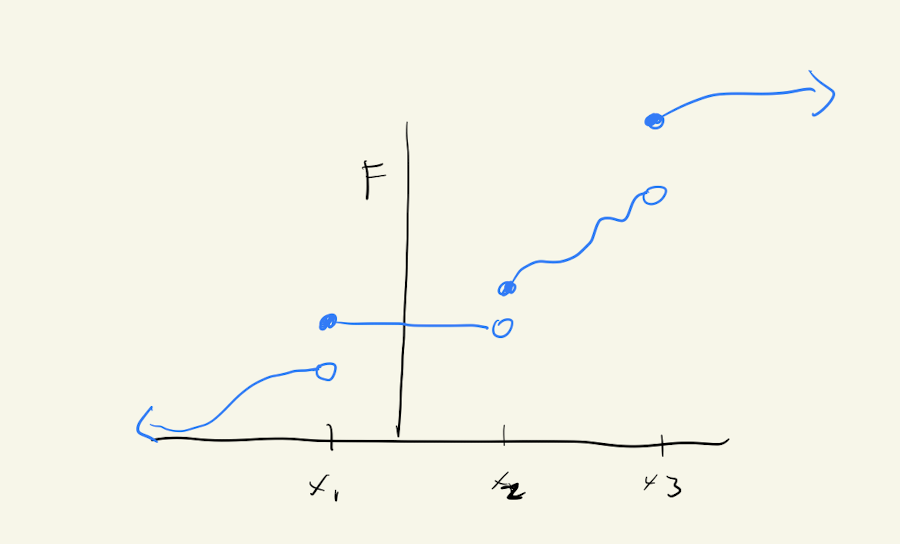
\includegraphics[width=.5\textwidth]{images/distribution_function_with_positive_mass_on_points_that_is_not_concentrated_on_a_countable_set}
 \caption{A distribution function with positive mass on points that is not concentrated on a countable set}	
\label{fig:distribution_function_with_positive_mass_on_points_that_is_not_concentrated_on_a_countable_set}
\end{figure}


%Figure \ref{fig:distribution_function_with_positive_mass_on_points_that_is_not_concentrated_on_a_countable_set} helps to illuminate how working with distribution functions will allow us to cover absolutely continuous, discrete, and mixed random variables in a single paradigm. 
   
\label{rk:continuity_at_a_point_iffi_measure_zero_at_a_point}
\end{remark}

\begin{remark}
The characterization of continuity in Remark \ref{rk:continuity_at_a_point_iffi_measure_zero_at_a_point} in terms of measure zero can be an interesting way to prove continuity, or prove the existence of functions with interesting properties.   For instance, take a countable set $S = \set{x_1, x_2, ...}$ and non-negative weights $\set{w_1, w_2, ...}.$ such that $\sum_i w_i < \infty$.   Then define $\mu(A) = \sum_{i} \set{w_i : x_i \in A}$.  Now $\mu$ is a Lebesgue-Stietljes measure (and is in fact a finite measure), since $\mu(I) < \infty$ for each bounded interval $I$. By taking $S$ to be the rationals, we have proven the existence of an increasing function $F : \R \to \R$ that is continuous on the irrationals and discontinuous on the rationals {\footnotesize [since each Lebesgue-Stieltjes measure determines a distribution function $F$ (up to additive constant), and the set of continuities is given by \eqref{eqn:continuity_at_a_point_iffi_measure_zero_at_a_point}]}.
\end{remark}

\begin{remark}{\remarktitle{Lebesgue-Stieltjes measures of intervals for continuous distribution functions}}
When a distribution function $F$ is continuous rather than simply right continuous, the properties in Proposition \ref{prop:properties_of_LS_measures} reveal that the Lebesgue-Stieltjes measure of an interval does not depend upon whether the intervals are open or closed, i.e. 
\begin{subequations}
\begin{align}
\mu(a,b] &= \mu(a,b) = \mu[a,b) = \mu[a,b] = F(b)-F(a) &&  \text{for } a \leq b \\
\mu(-\infty,x) &= \mu(-\infty,x] = F(x) - F(-\infty) && \text{for } x \in \R  \\
\mu(x,\infty) &= \mu[x,\infty) = F(\infty) - F(x) && \text{for } x \in \R  
\end{align}
\label{eqn:LS_measures_with_continuous_distribution_function_dont_care_about_intervals_being_open_or_closed}
\end{subequations}

We will informally summarize this as $\mu(a,b]=\mu(a,b)=\mu[a,b)=\mu[a,b]$, where we may take $a,b \in \overline{\R}$ as long as we aren't closing the interval at $\pm \infty$.
\label{rk:LS_measures_with_continuous_distribution_function_agnostic_to_open_vs_closed_intervals}
\end{remark}


\begin{remark}
Note that the properties in Proposition \ref{prop:properties_of_LS_measures} hold even though differences (between a set and a subset) and measures don't commute outside of finite measures.\footnote{See Theorem \ref{thm:basic_properties_of_finitely_additive_set_functions}.}  For instance, if we determine $F$ from the equivalence class by setting $F(-\infty)=0$, then property d) of Proposition \ref{prop:properties_of_LS_measures} says 
\[  \mu[a,b) = \mu(-\infty, b) - \mu(-\infty, a).\]
But we couldn't make that statement by the piece-and-difference decomposition (see Theorem \ref{thm:basic_properties_of_finitely_additive_set_functions}), since $\mu$ isn't necessarily finite.  Thus, continuity of measure lets claim things that the piece-and-difference decomposition does not.
\end{remark}



\subsection{Examples of Lebesgue-Stieltjes measures on $\R$}

\begin{example}{\remarktitle{Lebesgue measure}}
Under the identity distribution function ($F(x)=x$), we have $\mu(a,b]=F(b)-F(a)$.  This is known as Lebesgue measure.  Recall from Remark \ref{rk:LS_measures_with_continuous_distribution_function_agnostic_to_open_vs_closed_intervals} that since $F$ is continuous, we also have $\mu(a,b]=\mu(a,b)=\mu[a,b)=\mu[a,b]$.
\label{ex:Lebesgue_measure_as_example_of_Lebesgue_stieltjes} 
\end{example}

\begin{example}{\remarktitle{Generating Lebesgue-Stieltjes measures via integration}}
We can generate a large class of measures on $\B(\R)$ as follows.  Let $f$ be integrable (Riemann for now) on any finite interval, and define
\[ F(b) - F(a) = \ds\int_{a}^b f(t) \, dt\]
which determines $F$ up to an additive constant.   Then $F$ is a distribution function (as it is both increasing and continuous), so it gives rise to a Lebesgue-Stieltjes measure $\mu(a,b] = F(b) - F(a)$.  Lebesgue measure (Example \ref{ex:Lebesgue_measure_as_example_of_Lebesgue_stieltjes}) is a special case where $f \equiv 1$.  Once again, Remark \ref{rk:LS_measures_with_continuous_distribution_function_agnostic_to_open_vs_closed_intervals} reveals that by continuity of $F$, we have $\mu(a,b]=\mu(a,b)=\mu[a,b)=\mu[a,b]$.  
\end{example}

\paragraph{A non-example.} All Lebesgue-Stieltjes measures are sigma-finite. (To see this, simply set $\R = \cup_{n \in \mathbb{N}} (-n,n)$, and observe that $\mu(-n,n)<\infty$.). Here we provide an example of a sigma-finite measure that is not Lebesgue-Stieltjes.   First, let $\mu$ be concentrated on $S$ (i.e. $\mu(S^c)=0$), where we set $S= \set{1/n : n=1,2,...}$.    Take $\mu\set{1/n}=1/n$ for all $n$.  Since $\R = \cup_{n=1}^\infty {1/n} \cup S^c$, $\mu$ is sigma-finite.  However,
\[  \mu[0,1] \stackrel{\text{countable additivity}}{=} \ds\sum_{n=1}^\infty \df{1}{n} = \infty\]
and so $\mu$ is not a Lebesgue-Stieltjes measure. 
 
\subsection{Lebesgue measurable sets} \label{sec:Lebesgue measurable sets}

\begin{definition}
The completion of Lebesgue measure relative to $\B(\R)$ gives what is known as the \textit{Lebesgue measurable sets}, denoted $\L(\R)$.\footnote{See Section \ref{sec:completion_of_measure_spaces} for the definition of the completion of a measure space.}   
\end{definition}

Each Lebesgue measurable set is the union of a Borel set and a subset of a Borel set with Lebesgue measure zero.

\begin{remark}
The term ``Lebesgue measure" can be used to refer to

\begin{align*}
\mu : \; & \L(\R) \to \R^+
\intertext{as well as}
\mu : \; & \B(\R) \to \R^+
\end{align*}
\cite[pp.~37]{folland1999real},\cite{ash2000probability}.
\label{rk:lebesgue_measure_can_refer_to_the_function_whose_domain_is_the_borel_sets_or_whose_domain_is_the_lebesgue_measurable_sets}
\end{remark}


\subsection{$\S$ 1.4.6 Lebesgue-Stieltjes Measures on $\R^n$}

\subsubsection{Overview}
In $\R^n$, as with $\R$, is it possible to establish a one-to-one correspondence between Lebesgue-Stieltjes measures and distribution functions (up to some identification conditions).  However, the details are quite tedious.  

For our purposes, we will focus on
\begin{itemize}
\item Pointing out that, and motivating why, the definition of a distribution function must change in $\R^n$.
\item Showing that if $\mu$ is a \textit{finite} measure on the Borel sets of $\R^n$ and $F(x) = \mu(-\infty, x], x \in \R^n$, then $F$ is a distribution function on $\R^n$ and $\mu(a,b]$ can be provided in terms of it.     (The finite condition can be relaxed, but we omit this here.) %#= \Delta_{(a,b]} F$.
\item Providing some examples of Lebesgue-Stieltjes distribution functions in $\R^n$. 
%\item Stating the converse -- that if $F$ is a distribution on $\R^n$, there there is a unique Lebesgue-Stieltjes measure associated to it, with $\mu(a,b]$ determined by it. 	
\end{itemize}

 
\subsubsection{Definitions}
The definition of Lebesgue-Stieltjes measures on $\R^n$ parallels those on $\R$.

\begin{definition}
We define a \textit{right semi-closed interval} (or right semi-closed rectangle or right semi-closed box) in $\R^n$ as
\[ (a,b] :=	(a_1,b_1] \times ... \times (a_n, b_n]  = \set{x \in \R^n : a_1 < x_1 \leq b_1, ...., a_n < x_n \leq b_n }\]
\end{definition}


\begin{figure}[H]
\centering
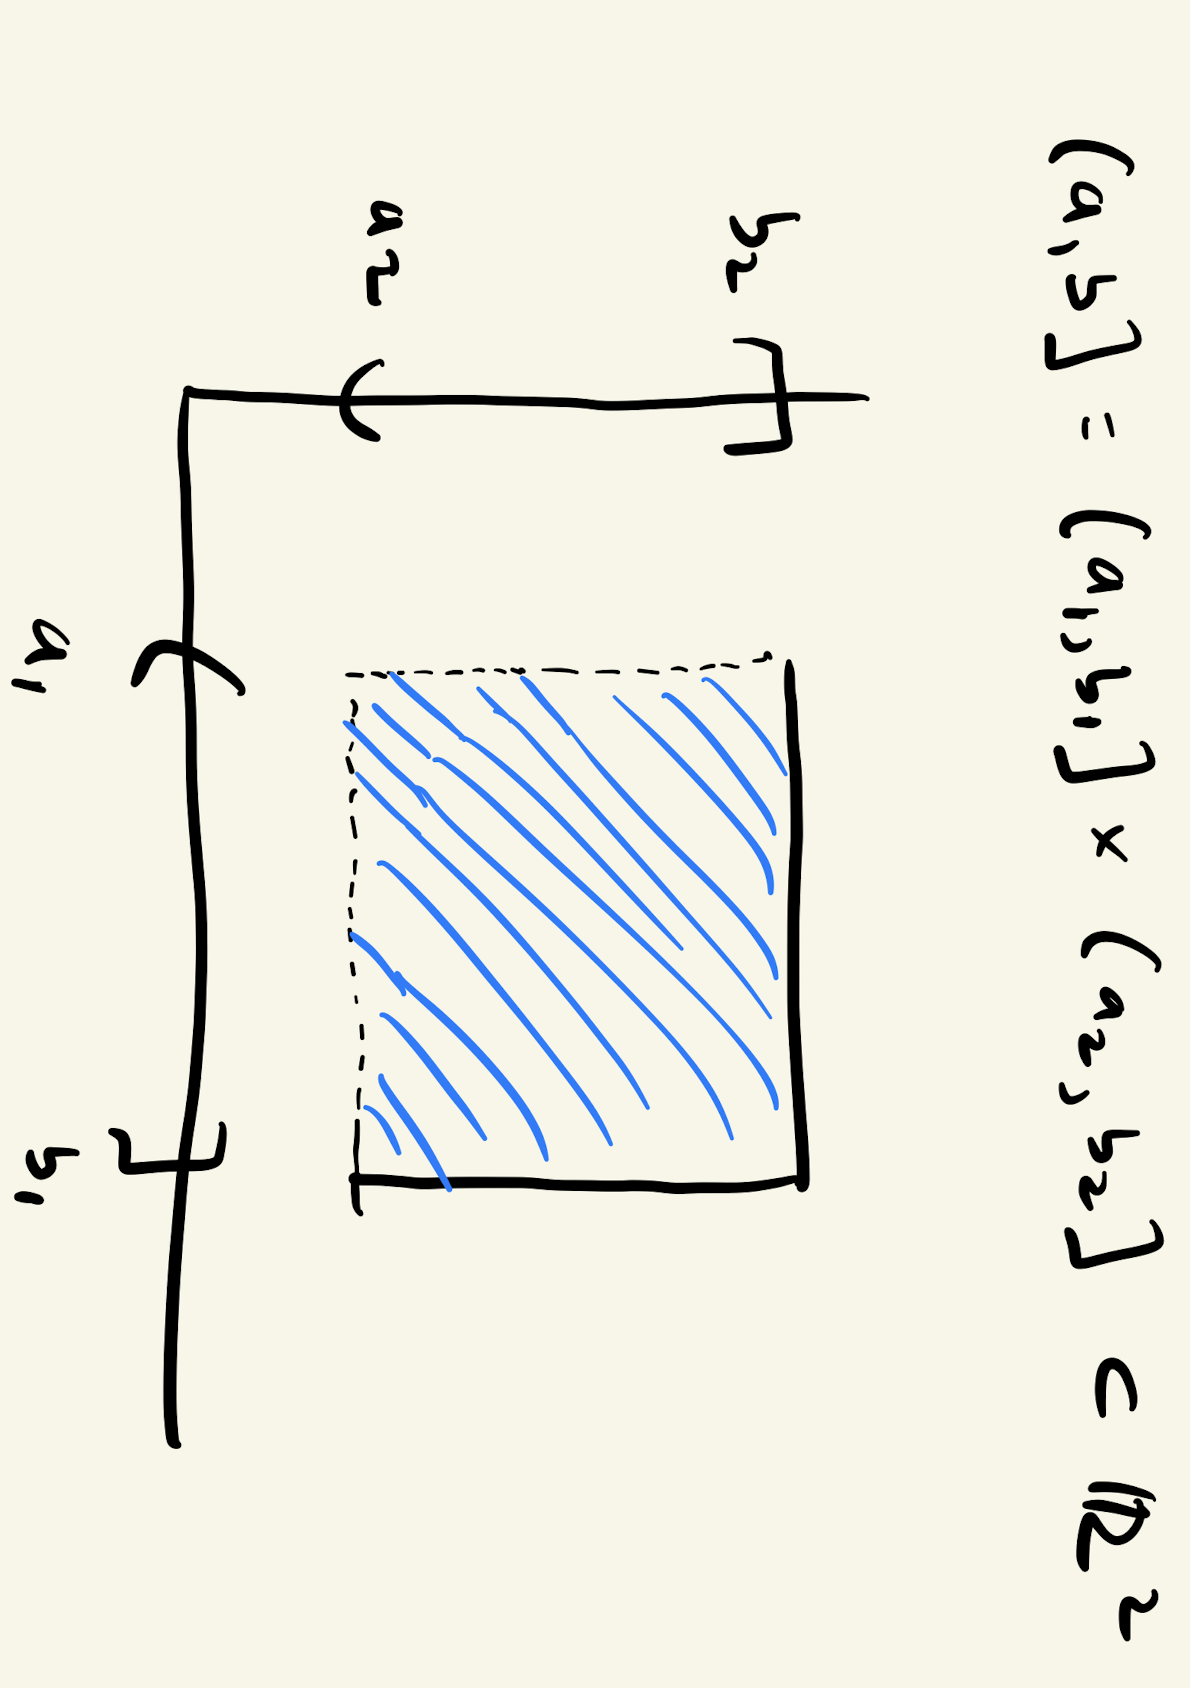
\includegraphics[angle=90, width=.3\textwidth]{images/rsc_rectangle_in_R2}	
\end{figure}

\begin{definition}
The \textit{vertices} of a right semi-closed interval in $\R^n$ are given by
\[ V(a,b] = \set{a_1,b_1} \times ... \times \set{a_n, b_n}\]
\label{def:vertices_of_rsc_interval_in_Rn}
\end{definition}

\begin{definition}
The \textit{Borel sets} of 	$\R^n$, denoted $\B(\R^n)$, are those sets which are members of the smallest sigma field containing all right semi-closed intervals $(a,b], a,b \in \R^n$. 
\end{definition}

\begin{definition}
A \textit{Lebesgue-Stieltjes measure} on $\R^n$ is a measure $\mu$ on $\B(\R^n)$ such that $\mu(I) < \infty$ for each bounded interval $I$. 	
\end{definition}

%We have established how to relate distribution functions and measures when the underlying space is $\R$.  When the underlying space is $\R^n$, the situation is different.

\subsubsection{From (finite) measures on $\B(\R^n)$ to distribution functions}
Recall that in $\R$, we observed the following relation between distribution functions  and Lebesgue-Stieltjes measures on right semi-closed intervals 
\begin{align*}
\mu(a,b] = F(b) - F(a), \quad a,b \in \R, a<b 
\labelit \label{eqn:measure_as_distribution_function_difference_for_motivating_LS_in_Rn}
\end{align*}
In particular, we observed that given $\mu$, we could construct an $F$ (up to additive constant) via the above relationship.   If we defined $F(-\infty) = 0$, then we could construct $F$ from $\mu$ directly via 
\[ F(x)=\mu(-\infty, x] = \mu(\omega \in \R : \omega \leq x) \]

We would like to to do the same for $\R^n$.  However, note that the equation 
\begin{align*}
\mu(a,b] = F(b) - F(a), \quad a,b \in \R^n, a<b 	
\labelit \label{eqn:measure_as_distribution_function_difference_for_motivating_LS_in_Rn}
\end{align*}
does \textit{not} hold anymore! To see this, let us define  $F : \R^n \to \R$ via 
\[  F(x) = \mu(-\infty, x] = \mu(\omega \in \R^n : \omega_1 \leq x_1, ..., \omega_n \leq x_n)\]

%{\footnotesize We note that that this parallels the situation in $\R$, where  we have $\mu(-\infty, a]=F(a)$ if we identify a member from the equivalence classes of distribution functions by assuming $F(-\infty)=0$.}


\begin{figure}[H]
\centering
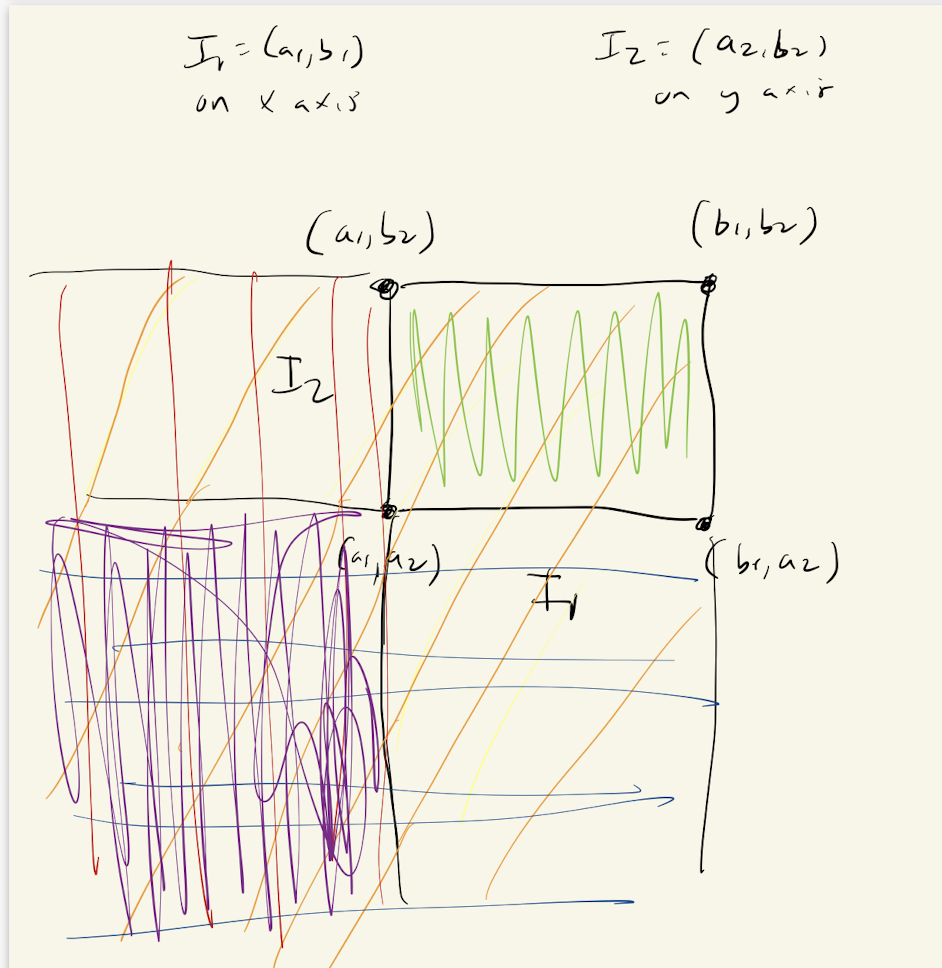
\includegraphics[width=.5\textwidth]{images/distribution_functions_in_Rn}	
\caption{Using a distribution function in $\R^2$ to measure the box $I_1 \times I_2$.}
\label{fig:distribution_functions_in_Rn}
\end{figure}


Now consider Figure \ref{fig:distribution_functions_in_Rn}. We see that if $(a,b] = I_1 \times I_2 = (a_1,b_1] \times (a_2, b_2]$, then 
\begin{align*}
\mu(a,b] &= F(b_1, b_2) - F(a_1, b_2) - F(b_1, a_2) + F(a_1, a_2)
\labelit \label{eqn:measure_of_rsc_interval_in_R2} \\
& \neq F(b_1, b_2) - F(a_1, a_2)
\end{align*}
(Note that we add back in the region that we had double subtracted.)

Now we generalize \eqref{eqn:measure_of_rsc_interval_in_R2} to a formula for measuring r.s.c. intervals in $n$ dimensions, rather than just $2$ dimensions.

\begin{theorem}
Let $\mu$ be a finite measure on $\B(\R^n)$. Define  $F : \R^n \to \R$ via $F(x) = \mu(-\infty, x] = \mu(\omega \in \R^n : \omega_1 \leq x_1, ..., \omega_n \leq x_n)$. Then 
\begin{alphabate}
\item We have 	
	\begin{align*}
	\mu(a,b] &= \Delta_{(a,b]} F  := \Delta_{b_1a_1} \cdots \Delta_{b_na_n} F(x_1, ..., x_n) 
	\labelit \label{eqn:measure_of_rsc_interval_in_Rn_via_distribution_function}
	\intertext{where}
	\Delta_{b_ia_i} G(x_1,...,x_n) &:= G(x_1,....,x_{i-1}, b_i, x_{i+1}, ..., x_n) - G(x_1,....,x_{i-1}, a_i, x_{i+1}, ..., x_n)
	\end{align*}
\item We have
	\begin{align*}
\Delta_{(a,b]} F = \sum_{v \in V(a,b]} (-1)^{\# \text{ of $a_i$'s in v}} \; F(v)
\labelit \label{eqn:computing_area_of_a_rectangle_via_a_distribution}	
	\end{align*}
where $V(a,b]$ are the vertices of $(a,b]$ (see Definition \ref{def:vertices_of_rsc_interval_in_Rn}). 
\end{alphabate}
\label{thm:measure_of_rsc_interval_in_Rn_via_distribution_function}
\end{theorem}

\begin{proof}
We prove part (a) and leave (b) to the reader.
\begin{align*}
\Delta_{b_na_n} &F(x_1, ..., x_n) = 	F(x_1,...,x_{n-1}, b_n) - F(x_1,...,x_{n-1}, a_n)\\
&=\mu(\set{\omega_1 \leq x_1, \; ..., \; \omega_{n-1} \leq x_{n-1}, \; \omega_{n} \leq b_{n}}) - \mu(\set{\omega_1 \leq x_1, \; ..., \; \omega_{n-1} \leq x_{n-1}, \;\omega_{n} \leq a_{n}}) \\
&=\mu(\set{\omega_1 \leq x_1, \; ..., \; \omega_{n-1} \leq x_{n-1}, \; a_n < \omega_{n} \leq b_{n}})
\end{align*}
where the last equality follows by the piece-and-difference decomposition of finite measures.

Similarly, 
\begin{align*}
\Delta_{b_{n-1}a_{n-1}} &\Delta_{b_na_n} F(x_1, ..., x_n) \\
&=\mu(\set{\omega_1 \leq x_1, \;..., \; \omega_{n-2} \leq x_{n-2}, \; a_{n-1} < \omega_{n-1} \leq b_{n-1}, \; a_n < \omega_{n} \leq b_{n}})
\end{align*}
Repeating this, we obtain
\[\Delta_{b_1a_1} \cdots \Delta_{b_na_n} F(x_1, ..., x_n) =  \mu(\set{a_1 < \omega_1 \leq b_1, \; ... \; a_n < \omega_{n} \leq b_{n}}) = \mu(a,b]\]

\end{proof}

\begin{notation}
What I call $\Delta_{(a,b]} F$ in \eqref{eqn:measure_of_rsc_interval_in_Rn_via_distribution_function} is called $F(a,b]$ by \cite{ash2000probability}.  See e.g. \cite[pp.28, or pp.149]{ash2000probability}.  I find Ash's notation completely puzzling.
\label{notation:ash_notation_for_multivariate_distribution_function_applied_to_an_rsc_interval}
\end{notation}



\begin{remark}
Note from the proof of Theorem \ref{thm:measure_of_rsc_interval_in_Rn_via_distribution_function} part (a) that the application of the $n$th difference operator restricts the set being measured to the bounds given in the $n$th dimension.  See Figure \ref{fig:applying_the_difference_operator_to_distribution_functions_in_R2}.

\begin{figure}[H]
\centering
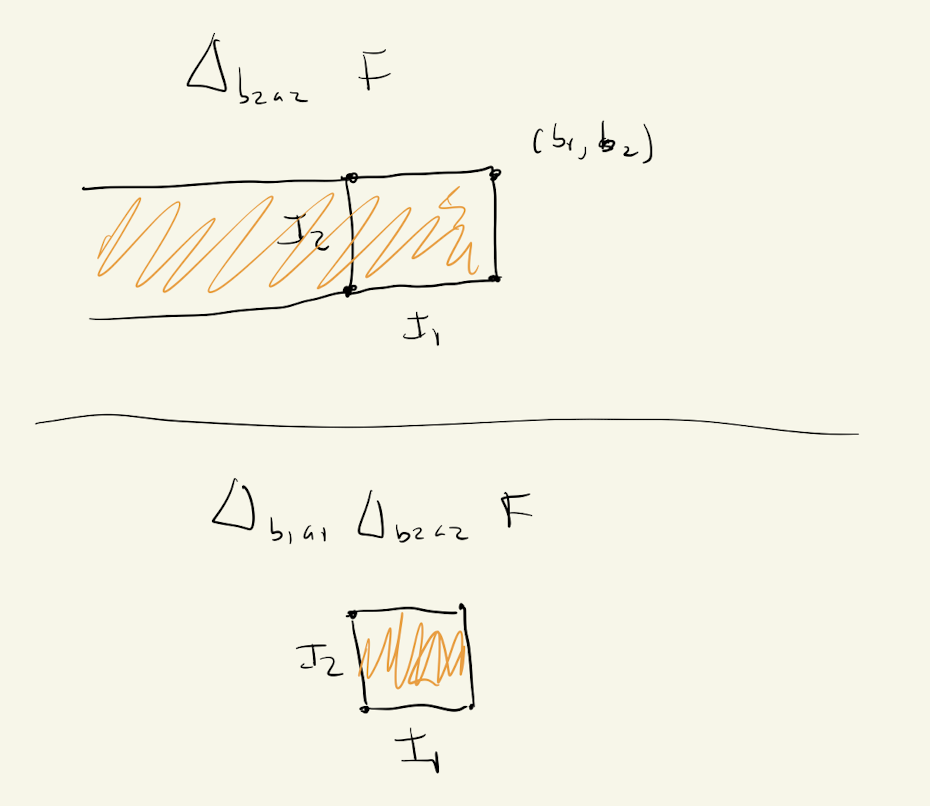
\includegraphics[width=.5\textwidth]{images/applying_the_difference_operator_to_distribution_functions_in_R2}	
\caption{Repeated applications of the difference operator to a distribution function in $\R^2$.}
\label{fig:applying_the_difference_operator_to_distribution_functions_in_R2}
\end{figure}


\end{remark}

\begin{remark}
Equation \eqref{eqn:computing_area_of_a_rectangle_via_a_distribution} tells us that we can measure any $n$-dimensional rectangle in $\R^n$ via $2^n$ evaluations of the distribution function. 
\end{remark}


\subsubsection{Defining distribution functions in $\R^n$}

When defining distribution functions on $\R^n$,  we must alter our notion of \textit{increasing}.     This is due to Theorem \ref{thm:measure_of_rsc_interval_in_Rn_via_distribution_function} part (a).

\begin{definition}
 A \textit{distribution function} on $\R^n$ is a map $F : \R^n \to \R$ that is:
 
 \begin{alphabate}
 \item \textit{increasing}, i.e. its increments must be non-negative in the sense that
 \begin{align*}
 \Delta_{(a,b]} F \geq 0 \quad \text{ for all r.s.c. intervals $(a,b]$}
 \labelit \label{eqn:increasing_condition_for_distribution_functions_on_Rn}
 \end{align*}



 \item \textit{right continuous}, that is
 \[ \ds\lim_{y \downarrow x} F(y) = F(x) \]
 where $y \downarrow x$ means $y_i \downarrow x_i$ for each $i=1,...,n$.
 \end{alphabate}
 \label{def:distribution_function_on_Rn}
 \end{definition}
 
 \begin{remark}
 Note that Definition \ref{def:distribution_function_on_Rn} defines increasing in a different manner than what might be intuitive:
 \[ F(y) \geq F(x) \; \text { if } \; y_i \geq x_i \quad \text{ for all } i=1,...,n\]
 However, such a condition would be insufficient to describe a distribution function in $\R^n.$ For an example of a distribution function that is right continuous and increasing in this sense, but which can assign negative measure to an interval, see pp. 6-7 of \cite{durrett2010probability}.
 \end{remark}

 \subsubsection{From distribution functions on $\R^n$ to Lebesgue-Stieltjes measures}
 
 \begin{theorem}
 Let $F$ be a distribution function on $\R^n$, and let $\mu(a,b] = F(a,b], a,b \in \R^n, a \leq b$. Then there is a unique extension of $\mu$ to a Lebesgue-Stieltjes measure on $\R^n$.	
 \end{theorem}
 
 \begin{proof}
 See text. 	
 \end{proof}

\subsubsection{Examples} \label{sec:examples_of_how_to_construct_lebesgue_stieltjes_measures_from_distribution_functions}

Here we provide some examples of how Lebesgue-Stieltjes measures can be constructed on $\R^n$ via distribution functions.

\begin{enumerate}
\item Let $F_1,F_2,...,F_n$ be distribution functions on $\R$, and define $F(x_1,...,x_n) = F_1(x_1) F_2(x_2) \cdots F_n(x_n)$.  Then $F$ is a distribution function on $\R^n$; it is clearly right-continuous, and it is increasing since
\[ \Delta_{(a,b]} F =\ds\prod_{i=1}^n [F(b_i) - F(a_i)] \geq 0 \]
	
A special case is where each $F_i$ is the distribution function corresponding to Lebesgue measure on $\B(\R)$.  Then each $F_i(x_i) = x_i$, and so we have
\[ F(x_1,...,x_n) = x_1x_2 \cdots x_n\]
This $\mu$ is \textit{Lebesgue measure} on $\B(\R^n)$.  Note that 
\[ \mu(a,b] = \Delta_{(a,b]} F = \ds\prod_{i=1}^n (b_i-a_i) \]
and more generally, the Lebesgue measure of any rectangular box is its volume (which can be seen by using a slight tweak to the arguments of parts (b)-(d) of the proof of Proposition \ref{prop:properties_of_LS_measures}). 
\item Let $f$ be any non-negative function from $\R^n$ to $\R$ such that 
\[ \ds\int_{-\infty}^\infty \cdots  \ds\int_{-\infty}^\infty f(x_1,...,x_n) \; dx_1 \cdots dx_n < \infty \]
(For now, we assume the integration is in the Riemann sense.)

Define 
\[ F(x) = \ds\int_{(-\infty,x]} f(t) dt \]
Then $F$ is a distribution function. It is continuous by the fundamental theorem of calculus, and it is increasing since
\[ \Delta_{(a,b]} F(x) = \ds\int_{a_1}^{b_1} \cdots  \ds\int_{a_n}^{b_n} f(x_1,...,x_n) \; dx_1 \cdots dx_n < \infty \]  
\end{enumerate}

%\begin{exercise}
%We wrote ``more generally, the Lebesgue measure of any rectangular box is its volume."  Show that, indeed, 
%\[  \mu(a,b]  = \mu(a,b) = \mu[a,b) = \mu[a,b] \]
%for Lebesgue measure on $\B(\R^n)$.  (Recall that we have shown that these equalities hold for Lebesgue measure on $\B(\R)$.)
%\end{exercise}

\begin{remark}

It may seem hard to verify \eqref{eqn:increasing_condition_for_distribution_functions_on_Rn}, the condition that a distribution function on $\R^n$ must be increasing.  Not to worry, the recipes above provide straightforward mechanisms for constructing distribution functions on $\R^n$ in which the condition will automatically be verified.
\end{remark}

\subsubsection{Summary}

Let us summarize.\footnote{This passage is basically a paragraph from \cite{ash2000probability} pp. 32 verbatim. However, we alter it slightly here to match our notation.} We have seen that if $F$ is a distribution function on $\R^n$, then there is a unique Lebesgue-Stieltjes measure determined by $\mu(a,b] = \Delta_{(a,b]} F, a \leq b$.  Also, if $\mu$ is a finite measure on $\B(\R^n)$ and $F(x) = \mu(-\infty, x], x \in \R^n$, then $F$ is a distribution function on $\R^n$ and $\mu(a,b] =  \Delta_{(a,b]} F, a \leq b$.   It is possible to associate a distribution function with arbitrary Lebesgue-Stieltjes measure on $\R^n$, and thus to establish a one-to-one correspondence between Lebesgue-Stieltjes measures and distribution functions (provided distribution functions with the same increments $\Delta_{(a,b)} F, a,b \in \R^n, a \leq b$ are identified).  However, the result will not be needed, and the details are quite tedious. 

%applying_the_difference_operator_to_distribution_functions_in_R2

% TODO: Define the difference operator, give theorem 1.4.8 but for (b) use the Durrett statement, prove (a) like my notes.  Skip the proof of (b).   Perhaps give the Ash statement for (b) in a remark.  Make a picture and remark for (a) giving the intuition: the $n$th application of the difference operator restricts the set being measured to the bounds given in the $n$th dimension.   Then define distribution functions in R^n.  Finally give the extension statement for $R^n$. 

\subsection{Properties of Borel sets under Lebesgue measure} \label{sec:properties_of_borel_sets}

Below we show some properties of Borel sets that hold under Lebesgue measure.  How can we accomplish this?  After all, the Borel sets are rather abstractly defined, and although we have been generating them via disjoint unions of r.s.c intervals, they also contain many types of members (e.g., proper open intervals, proper closed intervals, and singletons; bizarre sets like the Cantor set; inverse images of Borel measurable sets under Borel measurable functions; etc.).

To prove that such properties hold, we can take a standard tact: use the the Monotone Class Theorem,  to show that the Borel sets have some property.  Using this approach, we can show that a property holds for \textit{all} Borel sets if we can just show that the property holds for some field generating the Borel sets (e.g., $\F_0 := \set{\text{disjoint unions of } (a,b], a,b \in \R^n }$) -- a much more tangible object to work with.


\begin{remark}{\remarktitle{Using the Monotone Class Theorem to prove that the Borel sets have some property}}
Suppose you want to show that all Borel sets $\B(\R^n)$ have some property $P$.  Define ``good sets" as those that satisfy the property
\[ \G := \{ B \in \B(\R^n) : B \text{ has property } P \} \]
The strategy is then to simply
\begin{enumerate}
\item Show $\G$ contains $\F_0 := \set{\text{disjoint unions of } (a,b], a,b \in \R^n }$.
\item Show $\G$ is a monotone class.  
\end{enumerate}	 
\label{rk:monotone_class_theorem_for_executing_good_sets_strategy_with_borel_sets}
\end{remark}


This is a particular version of the Good Sets Strategy (see Remark \ref{rk:monotone_class_theorem_for_executing_good_sets_strategy}) in the special case where the $\sigma$-field of interest is the Borel sets (and where we take the field generating them to be $\F_0$).  As pointed out in Remark \ref{rk:monotone_class_theorem_for_executing_good_sets_strategy}, this strategy is very much like induction.  Step \#1 is the ``base" step and Step \#2 is the ``induction" step.

For examples where this strategy is used, see the  Approximation Theorem for Borel sets (Theorem \ref{thm:approximation_theorem_for_borel_sets}) or the proof that Lebesgue measure is translation invariant (Proposition \ref{prop:Lebesgue_measure_is_translation_invariant}). We begin with the Approximation Theorem for Borel sets.  This theorem shows that under appropriate conditions, a Borel set can be approximated from below by a compact set, and from above by an open set. 

%\begin{remark}{\remarktitle{Using the Monotone Class Theorem to prove that the Borel sets have some property}} The Borel sets are rather abstract, and also contain many types of members (e.g., proper open intervals, proper closed intervals, singletons, bizarre sets like the Cantor set, etc.).  The MCT gives us a mechanism for showing that some property holds for \textit{all} Borel sets if we can just show that the property holds for some field generating the Borel sets (e.g., $\F_0 := \set{\text{disjoint unions of } (a,b], a,b \in \R^n }$) -- a much more tangible object to work with.  The strategy that is often used is a variant of the Good Sets strategy (see Remark \ref{rk:monotone_class_theorem_for_executing_good_sets_strategy}):  we consider the class of sets that have some desired property, and show that it is a monotone class and contains $\F_0$.  By the Monotone Class Theorem, these two facts are sufficient to prove that some property holds for all Borel sets.  For examples where this is used, see the  Approximation Theorem for Borel sets (Theorem \ref{thm:approximation_theorem_for_borel_sets}) or the proof that Lebesgue measure is translation invariant (Proposition \ref{prop:Lebesgue_measure_is_translation_invariant}).
%\label{rk:utility_of_montone_class_theorem}	
%\end{remark}

%\subsubsection{$\S$ 1.4.11 Approximation theorem for Borel sets}



\begin{theorem}
\textbf{(Approximation Theorem for Borel sets).} If $\mu$ is a $\sigma$-finite measure on $\B(\R^n)$, then for each $B \in \B(\R^n)$,
\begin{alphabate}
\item $\mu(B) = \sup \set{\mu(K) : K \subset B, K \text{ compact}}$
\item If $\mu$ is in fact a Lebesgue-Stieltjes measure, then
\[ \mu(B) = \inf \set{\mu(V) : V \supset B, V \text{ open}}\]
\item There is an example of a $\sigma$-finite measure on $\B(\R^n)$ that is not a Lebesgue-Stieljes measure for which (b) fails.
\end{alphabate}
\label{thm:approximation_theorem_for_borel_sets}	
\end{theorem}

\begin{proof}
\;
\begin{alphabate}
\item We prove (a) for finite measures.   For the extension to $\sigma$-finite measures, see the text.  

We use the Monotone Class Theorem to show that all Borel sets have the desired property. Let $\G$ be the class of subsets that have the desired property.\footnote{The reader may recognize that we are using the ``good sets" strategy.  See Section \ref{sec:good_sets_strategy} and Remark \ref{rk:utility_of_montone_class_theorem}.} 
	\begin{itemize}
	\item \textit{First, observe that $\G$ contains all compact sets.}  If $K$ is a compact set, then $\mu(K)$ is an upper bound on $\set{\mu(K') : K' \subset K, K' \text{ compact}}$ by monotonicity {\footnotesize [$\mu(K) \geq \mu(K') \text{ for } K' \subset K,  K' \text{ compact}$].}  It is also the least upper bound since for each $\epsilon$, there is a compact $K' \subset K$ satisfying $\mu(K') > \mu(K) - \epsilon$. {\footnotesize [Just take $K'=K$].}  
	\item \textit{Next, we show that $\G$ is a monotone class.}  So we need to show that (i) if $B_n \in \G$ and $B_n \downarrow B$ then $B \in \G$ and (ii) if $B_n \in \G$ and $B_n \uparrow B$ then $B \in \G$.  
		\begin{itemize}
		\item[(i)] Since each $B_n \in \G$, by definition of supremum (see Remark \ref{rk:usage_of_alternate_characterization_of_inf_and_sup}), we can find $K_n \subset B_n$, $K_n$ compact, such that 
		\[\mu(B_n) \leq \mu(K_n) + \epsilon 2^{-n}\]
		Set $K=\cap_{n=1}^\infty K_n$.   Then
		\begin{align*}
		\mu(B) - \mu(K) &= \mu(B-K) && \tinytext{piece-and-difference, $\mu$ finite} \\
		&\stackrel{1}{\leq} \mu(\cup_{n=1}^\infty (B_n-K_n)) && \tinytext{DeMorgan, monotonicity}\\
		&\leq \sum_{n=1}^\infty \mu(B_n - K_n) && \tinytext{countable subadditivity} \\
		&= 	\sum_{n=1}^\infty \mu(B_n) - \mu(K_n) && \tinytext{piece-and-difference, $\mu$ finite} \\
		&= \epsilon 
		\end{align*}
		{\footnotesize [For more detail, Equation (1) applies because $B - \cap_{n=1}^\infty K_n \stackrel{\text{DeMorgan}}{=} \cup_{n=1}^\infty (B-K_n) \stackrel{B \subset B_n}{\subset} \cap_{n=1}^\infty (B_n - K_n)$.]} \\
		
		So for all sets $B$ formed by $B_n \downarrow B$ for $B_n \in \G$, we have that $\mu(B)$ satisfies the second property of the supremum (see Definition \ref{def:supremum_and_infimum}).  {\scriptsize [It satisfies the first property immediately since $K_n \subset B_n  \implies \cap_{n=1}^\infty K_n \subset \cap_{n=1}^\infty  B_n$, so by monotonicity $\mu(K) \leq \mu(B)$, and so $B$ is an upper bound.]} 
		\item[(ii)]  Up to reader or see text for proof. 	
		\end{itemize}
	\item \textit{Now we show that $\G$ contains $\F_0 := \set{\text{disjoint unions of } (a,b], a,b \in \R^n}$}.  Consider that 
	\[ (a,b] = \bigcup_{n=1}^\infty \explaintermbrace{compact}{ \big[a+\frac{1}{n}, b \big] } \]	
	So $[a+1/n, b] \uparrow (a,b]$.  And since $(a,b]$ is the limit of an increasing sequence of compact sets, $(a,b] \in \G$ by the first two bullet points.  A similar argument holds for disjoint unions of sets which have the form $(a,b]$.  
	\item \textit{Now we use the Monotone Class Theorem to finish the proof.} By the previous bulletpoints, $\G$ contains $\F_0 := \set{\text{disjoint unions of } (a,b], a,b \in \R^n}$, and $\G$ is a monotone class.  So by the Monotone Class Theorem (Theorem \ref{thm:monotone_class_theorem}), $\G$ contains $\sigma(\F_0) = \B(\R^n)$.\footnote{In other words, \textit{all} Borel sets are are ``good" - they have the property stated in part (a).}  
	\end{itemize}


\item We prove part (b) for finite measures.  For the extension to $\sigma$-finite measures, see the text.

We have 
\begin{align*}
\mu(B) & \stackrel{1}{\leq}	\inf \set{\mu(V) : V \supset B, V \text{ open}} && \tinytext{by monotonicity and Definition \ref{def:supremum_and_infimum}} \\
 & \stackrel{2}{\leq}	\inf \set{\mu(K^c) : K^c \supset B, K \text{ compact}} && \tinytext{by monotonicity and Proposition \ref{prop:sup_and_inf_for_subsets_are_tighter}} \\
 &= \inf \set{\mu(\R^n) - \mu(K) : K \subset B^c, K \text{ compact}} && \tinytext{by piece-and-difference, $\mu$ finite} \\
 & \stackrel{3}{=}	\mu(\R^n) - \sup \set{\mu(K) : K \subset B^c, K \text{ compact}} && \tinytext{by Proposition \ref{prop:sup_and_inf_for_minkowski_sum_and_diff}} \\
  & =	\mu(\R^n) - \mu(B^c)  && \tinytext{by part (a)}\\
&= \mu(B)
\end{align*}
For more details, Equation (1) holds since, by monotonicity, the LHS is a lower bound on the RHS, so the statement must be true by definition of infimum. Equation (2) holds since the LHS is a smaller set than the RHS (because not every open set is the complement of a compact set)\footnote{Recall that in $\R^n$, a compact set is both closed \textit{and} bounded.}, and the infimum can only increase on subsets by Proposition \ref{prop:sup_and_inf_for_subsets_are_tighter}. Equation (3) holds by writing $\mu(K^c) = \mu(\R^n) - \mu(K)$.  This has the form of a Minkowski set difference $A = \set{c} - B$, where $c$ is a singleton.  So we have $\inf A = \inf ( \set{c} - B) \stackrel{Prop. \ref{prop:sup_and_inf_for_minkowski_sum_and_diff}}{=} \inf \set{c} - \sup B = c - \sup B$. 
\item See the text.
\end{alphabate}
 
 \end{proof}

%\subsubsection{Translation Invariance of Lebesgue Measure}

\begin{proposition}
\textbf{(Translation Invariance of Lebesgue Measure.)} Lebesgue measure is translation invariant.  That is, if $B \in \L(\R^n)$ and $c \in \R^n$, then $B+c \in  \L(\R^n)$ and $\mu(B+c)=\mu(B)$, where $\mu$ is Lebesgue measure.	
\label{prop:Lebesgue_measure_is_translation_invariant}
\end{proposition}

\begin{proof}
We prove the statement for $\B(\R^n)$ and leave the extension to $\L(\R^n)$ to the reader. We shall use the Monotone Class Theorem as our vehicle for executing the Good Sets Strategy (see Remark \ref{rk:monotone_class_theorem_for_executing_good_sets_strategy}).  That is, we will let $\G$ be the class of ``good sets" that have the desired property. Then we must show: (a) that $\G$ is a monotone class and (b) that $\G$ contains $\F_0 = \set{\text{disjoint union of sets of the form } (a,b], a, b \in \R^n}$. We will use this strategy twice, to show: (1) that $B \in \B(\R^n)$ and $c \in \R^n$ implies $B+c \in  \B(\R^n)$  (2) that $\mu(B+c)=\mu(B)$ for all $B \in \B(\R^n)$.  

\begin{enumerate}
\item We want to show that $B \in \B(\R^n) \implies B+c \in \B(R^n)$.  Let $\G$ be the sets where the property holds.
	\begin{alphabate}
	\item Consider a sequence $B_n \uparrow B$ such that $B_n \in \G$.  That is, by hypothesis, we have $B_n \in \B(\R^n) \implies B_n+c \in \B(R^n)$.  Then 
	\[  B+c = (\bigcup_{n=1}^\infty B_n) + c = \bigcup_{n=1}^\infty \explaintermbrace{\quad in $ \B(\R^n)$ \, by hypothesis}{(B_n + c)} \explaintermbrace{\quad by $\sigma$-field}{\in \B(\R^n)}\]
	So $B \in \G$.
	\item This property holds on $\F_0$; that is $\G \supset \F_0$.   Given $(a,b] \in \F_0, (a,b]+c = (a+c,b+c] \in \F_0$.  A similar statement holds for disjoint unions of r.s.c. intervals. 
	\end{alphabate}
\item We want to show that $\mu(B+c)=\mu(B)$ for all $B \in \B(\R^n)$.
	\begin{alphabate}
	\item Let $\G$ be the sets where the property holds. We show $\G$ is a monotone class. \\
	 
	 First, we handle increasing sequences. So we want to show $B_n \in \G, B_n \uparrow B \implies B \in G$.   Now by hypothesis, $\mu(B_n + c) = \mu(B_n)$.  So 
	 \begin{align*}
	 \mu(B+c) &=  \mu \big( \cup_{n=1}^\infty (B_n)+c \big)  && \tinytext{def. of $B$} \\
	  &=  \mu \big( \cup_{n=1}^\infty (B_n+c) \big)  && \tinytext{def. of union and +; still an increasing sequence} \\
	 &= \ds\lim_{n \to \infty} \mu(B_n+c)  && \tinytext{continuity from below} \\
	 &= \ds\lim_{n \to \infty} \mu(B_n) && \tinytext{hypothesis} \\
	 &= \mu(B) && \tinytext{continuity from below}
	 \end{align*}
 
 	Now we handle decreasing sequences.  So we want to show $B_n \in \G, B_n \downarrow B \implies B \in G$.  We could use the same argument as above with continuity from above instead of continuity from below, but continuity from above only applies for sets with finite measure.  However, Lebesgue measure is $\sigma$-finite, so we can handle this problem in the standard way.\footnote{In particular, we write $\Omega = \cupdot_{n=1}^\infty \Omega_n$ where $\mu (\Omega_n) < \infty$.\footnote{Recall that we can represent any union as a disjoint union; see Section \ref{sec:representing_unions_as_disjoint_unions}.}  Then we define a finite measure $\mu_n$ via $\mu_n(A) := \mu(A \cap \Omega_n)$.  We have 
 		\[ \mu(A) = \sum_{n=1}^\infty \mu_n(A), \quad (*)\]
 		since $\mu(A) = \mu(\cupdot A \cap \Omega_n) = \sum_n \mu(A \cap \Omega_n) = \sum_n \mu_n(A)$.
 		
 		Now, using the continuity from above argument for finite measures, we have 
 			\[ \mu_n(B+c) = \mu_n(B), \quad (+)\]
 			
 		And so
 		\[\mu(B+c) \stackrel{(*)}{=} \sum_n \mu_n (B+c)   \stackrel{(+)}{=}  \sum_n \mu_n(B) \stackrel{(*)}{=} \mu(B)  \]
 	}
% 	 \begin{align*}
%	 \mu(B+c) &\leq \mu(B) + \mu(c) && \tinytext{countable subadditivity} \\
%	 &= \ds\lim_{n \to \infty} [\mu(B_n)] + \mu(c) && \tinytext{continuity from below} \\
%	 &= \ds\lim_{n \to \infty} [\mu(B_n) + \mu(c)] && \tinytext{limit properties} \\
%	 &= \ds\lim_{n \to \infty} [\mu(B_n)] && \tinytext{hypothesis} \\
%	 &= \mu(B) && \tinytext{continuity from below}
%	 \end{align*}
% 
% 	\red{I AM ON DRUGS, THIS DOESNT HOLD}
	\item Now we show that $\G$ contains $\F_0$. The property certainly holds for r.s.c intervals; that is, $\mu(a+c,b+c] = \mu(a,b]$. \footnote{ For example, in $\R$, we have
	\[ \mu\big( (a,b] + c \big) = \mu\big( (a+c,b+c]\big) =(b+c) - (a+c) = b-a = \mu(a,b]\] 
	}  For Lebesgue measure on $\R^n$, the distribution function is $F(x_1, ..., x_n) = x_1 \cdots x_n$, and so $\mu (a,b] = \Delta_{b_1 a_1} \cdots \Delta_{b_n a_n} [x_1 \cdots x_n]$. Now note that
		\begin{align*}
		\Delta_{b_i + c_i, a_i+c_i} [x_1 \cdots x_n] &= x_1 \cdots x_{i-1} \bigg( (b_i + c_i) - (a_i + c_i)  \bigg) x_{i+1} \cdots x_n \\
		& = x_1 \cdots x_{i-1} \bigg( b_i - a_i  \bigg) x_{i+1} \cdots x_n \\
		&= \Delta_{b_i a_i} [x_1 \cdots x_n]  
		\end{align*}
	So $\Delta_{b_i + c_i, a_i+c_i} = \Delta_{b_i, a_i}$ for each $i=1,..n$.  Thus,  
	\[ \mu(a+c,b+c] = \Delta_{b_1+c_1, a_1 +c_1} \cdots \Delta_{b_n+c_n, a_n+c_n} [x_1 \cdots x_n] = \Delta_{b_1 a_1} \cdots \Delta_{b_n a_n} [x_1 \cdots x_n] = \mu(a,b] \] 
	A similar proof holds for disjoint unions of r.s.c intervals.
	\end{alphabate}
\end{enumerate}

\end{proof}

\subsection{A set that is not Lebesgue measurable} \label{sec:set_that_is_not_Lebesgue_measurable}

\begin{proposition}
Call $x,y \in \R$ equivalent iff $x-y \in \mathbb{Q}$.\footnote{So, for example, some equivalence classes are:
\begin{itemize}
\item $e \sim e + \frac{1}{10} \sim e - \frac{1}{10} \sim e+\frac{50}{3} \sim ...$
\item  $\pi \sim \pi + \frac{1}{10} \sim \pi - \frac{1}{10} \sim \pi+\frac{50}{3} \sim ...$
\item $1 \sim 1 + \frac{1}{10} \sim 1 - \frac{1}{10} \sim 1 +\frac{50}{3} \sim ...$
\end{itemize}
} Define $A \subset [0,1]$ as a set containing one member from each class. (This set exists by axiom of choice.) Then $A$ is not Lebesgue measurable.

\label{prop:existence_of_set_that_is_not_Lebesgue_measurable}
\end{proposition}

\begin{proof}
\begin{alphabate}
\item First, we show that we can partition the reals as $\R = \bigcupdot_{q \in \mathbb{Q}} (q+A)$.  
	\begin{itemize}
		\item \textit{(disjointedness)} Suppose $x \in q+A$ and $x \in r+A$ for some $r,q \in \mathbb{Q}, r \neq q$.  Then $\exists\, a_1,a_2 \in A : q + a_1 = r + a_2 \implies a_1 - a_2 = r - q$.   Now since $r \neq q$, we know that $a_1$ and $a_2$ are not the same.  But they are in the same equivalence class, since $r-q \in \mathbb{Q}$. This  contradicts how $A$ was constructed.
		\item \textit{(containment)} We show $\R \subset \bigcupdot_{q \in \mathbb{Q}} (q+A)$ (as the other direction is obvious).  If $x \in \R$ and $a_x$ is its representative in $A$, then $x-a_x = q \in \mathbb{Q}$, and so $x \in q + A$. %x is in A translated by q.
	\end{itemize}
\item Now we note that since $A \subset [0,1]$, we have 
\[ \bigcupdot_{q \in \mathbb{Q}, 0 \leq q \leq 1} (q + A) \subset [0,2] \]
So 
\[ 2 = [0,2] \stackreltext{subadditivity}{\geq} \mu\bigg(\bigcupdot_{q \in \mathbb{Q}, 0 \leq q \leq 1} q + A \bigg)  = \ds\sum_{q \in \mathbb{Q}, 0 \leq q \leq 1} \mu(q+A) \stackreltext{translation invariance}{=} \ds\sum_{q \in \mathbb{Q}, 0 \leq q \leq 1}  \mu(A) \]
This implies $\mu(A) = 0$, since the RHS of this equation is a countable sum of a constant, and so can only take on values $0$ or $\infty$.
	
But then 
\[ \infty = \mu(\R) \stackreltext{part (a)}= \mu \bigg(\bigcupdot_{q \in \mathbb{Q}} (q+A) \bigg)
= \ds\sum_{q \in \mathbb{Q}} \mu(q+A) 
 \stackreltext{translation invariance}{=}   \ds\sum_{q \in \mathbb{Q}} \mu(A) \stackreltext{see above}{=} 0. \;    \contradiction \]

\end{alphabate}

	
\end{proof}

\begin{remark}
The proof of Proposition \ref{prop:existence_of_set_that_is_not_Lebesgue_measurable} only used the following two properties of Lebesgue measure:
\begin{itemize}
\item translation invariance
\item finiteness on bounded intervals %(note that the argument in part (b) would go through for any bounded interval $[a,b]$ by the choice of bounds on $A$ and on the rationals used in part (b)). % Commented this out because it's outdated and possibly no longer relevant
\end{itemize}
Therefore, our argument shows that there cannot be a translation invariant measure $\lambda$ (except $\lambda \equiv 0$) on the class of all subsets of $\R$ such that $\lambda(I) < \infty$ for all bounded intervals $I$.
\label{rk:implications_of_existence_of_set_that_is_not_Lebesgue_measurable}
\end{remark}

% Commented the question out because it's outdated and possibly no longer relevant
%\begin{question}
%Our discussion in Remark \ref{rk:implications_of_existence_of_set_that_is_not_Lebesgue_measurable} parallels that of \cite{ash2000probability} pp. 35.  But haven't we actually proved a stronger result - namely that there cannot be a translation invariant measure $\lambda$ (except $\lambda \equiv 0$) on the class of all subsets of $\R$ such that $\lambda(I) < \infty$ for \textit{any} bounded interval $I$?
%\end{question}

\section{$\S$ 1.5 Measurable functions and Integration}

In this section, we will introduce the general theory of integration of a function with respect to a general measure, as introduced by Lebesgue.  We will refer to this as \textit{integration} or \textit{Lebesgue integration}. We use use \textit{(Lebesgue) integration against Lebesgue measure} to refer to the special case of integrating a function defined on a sub-domain of the real line with respect to the Lebesgue measure.   %  Some authors reserve the term \textit{Lebesgue integration} for  the special case of integration of a function defined on a sub-domain of the real line with respect to the Lebesgue measure, and refer to integration against arbitrary measure as \textit{abstract Lebesgue integration}.  We will differentiate between the general and special cases by referring to \textit{Lebesgue integration} (which can be against arbitrary measure) and \textit{Lebesgue integration against Lebesgue measure}.

\subsection{Intuition\footnote{Here we borrow freely from some sections of Wikipedia.}} \label{sec:intuition_on_Lebesgue_integration}

Folland summarizes the difference between the Riemann and Lebesgue approaches thus: ``to compute the Riemann integral of $f$, one partitions the domain [...] into subintervals", while in the Lebesgue integral, ``one is in effect partitioning the range of $f$ " \cite{folland1999real}.

Figure \ref{fig:Lebesgue_vs_Riemann} compares how the Riemann and Lebesgue approaches would approximate the area under the curve of a function $f : \R \to \R$. 

\begin{figure}[H]
\centering 
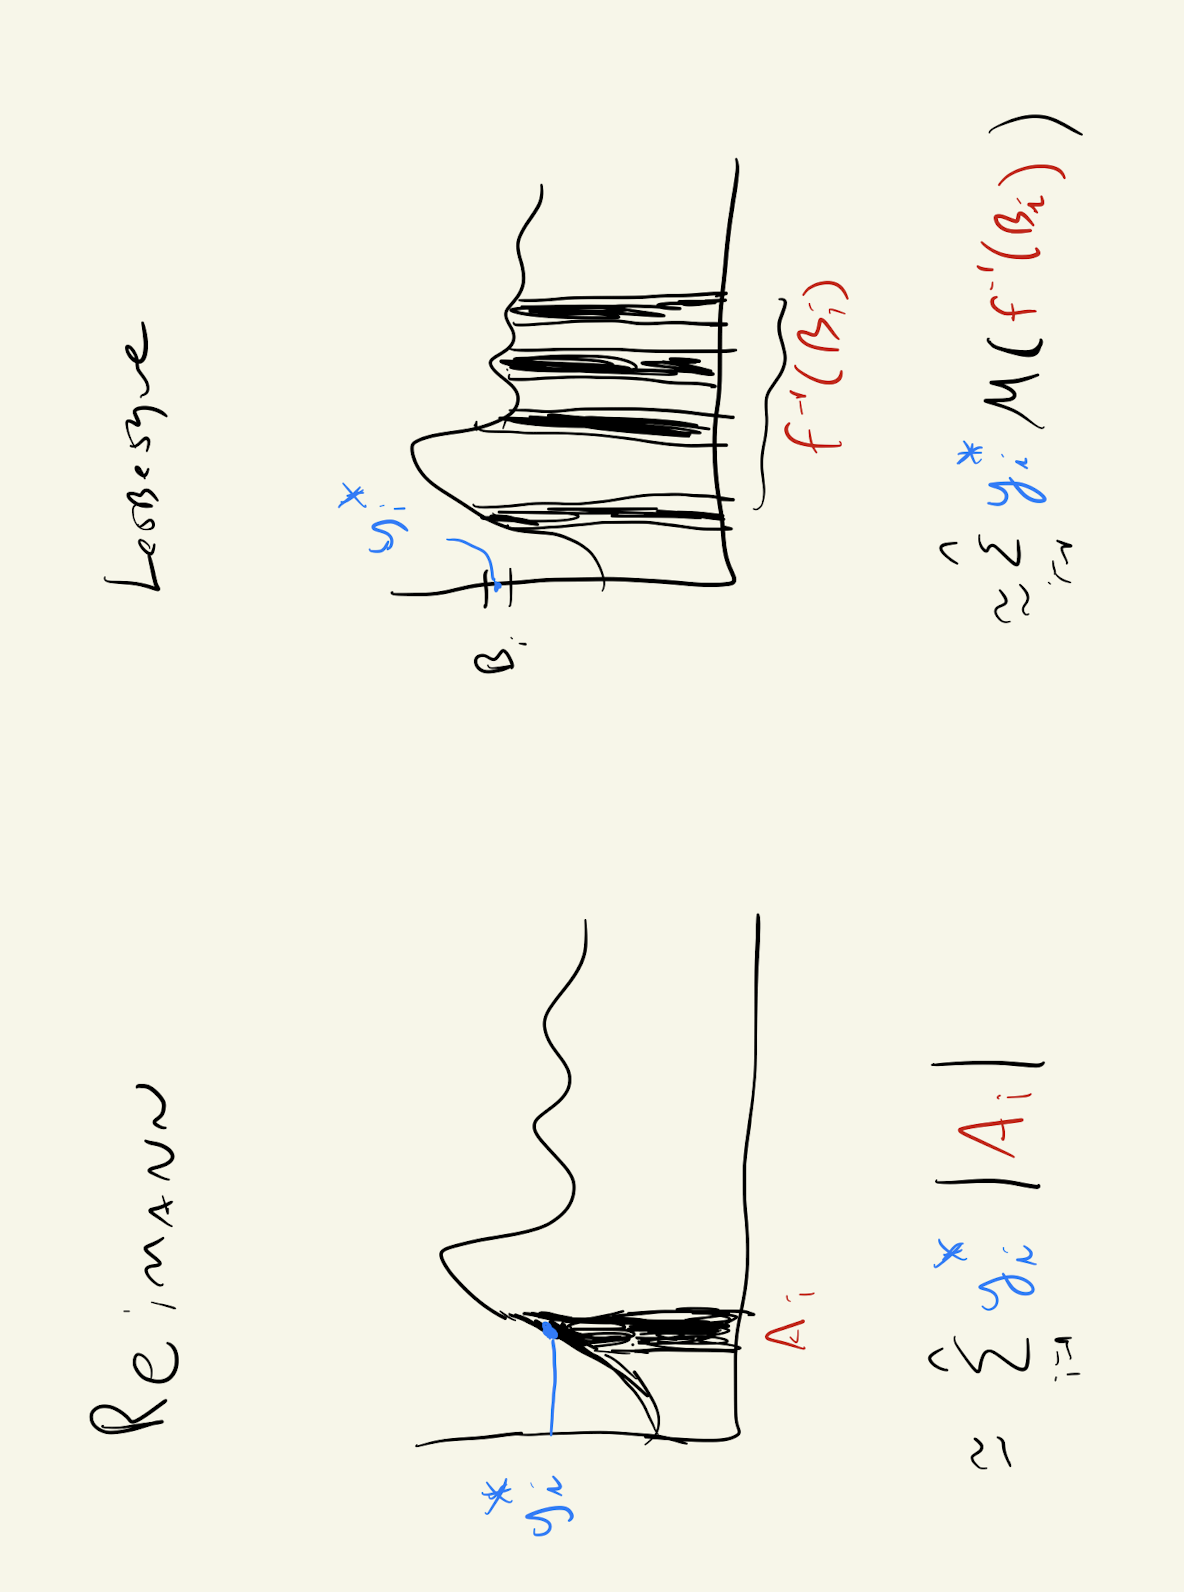
\includegraphics[width=.7\textwidth, angle=270]{images/Lebesgue_vs_Riemann}
\caption{Illustrating the fundamental differences between Riemann and Lebesgue integration}
\label{fig:Lebesgue_vs_Riemann}
\end{figure}

 In particular, notice:
\begin{enumerate}
\item Lebesgue integration partitions the range of $f$, whereas Riemann integration partitions the domain of $f$. As a result, the Lesbegue approach provides \textit{adaptive grouping} when computing the area under the curve as the sum over $n$ contributions.  Whereas a function can vary a lot in Riemann subintervals of the form $A_i = (a_i,b_i)$, in the Lebesgue approach, the function will have controlled amount of variation for each of the $n$ contributions.  While the approaches give equivalent answers for sufficiently nice functions (like continuous functions), the Lebesgue definition makes it possible to calculate integrals for a broader class of functions. For example, as we will see, the \textit{Dirichlet function}, which is 0 where its argument is irrational and 1 otherwise, has a Lebesgue integral, but does not have a Riemann integral.

Lebesgue summarized his approach to integration in a letter to Paul Montel:
\begin{quotation}
I have to pay a certain sum, which I have collected in my pocket.  I take the bills and coins out of my pocket and give them to the creditor in the order I find them until I have reached the total sum. This is the Riemann integral. But I can proceed differently. After I have taken all the money out of my pocket I order the bills and coins according to identical values and then I pay the several heaps one after the other to the creditor. This is my integral.
\end{quotation}



The insight is that one should be able to rearrange the values of a function freely, while preserving the value of the integral.  This process of rearrangement can convert a very pathological function into one that is ``nice" from the point of view of integration, and thus let such pathological functions be integrated.

\item The Riemann approach implicitly assumes that sets in the domain have sizes that are given by Lebesgue measure ($\mu(A) = |A|)$, whereas the Lebesgue approach allows sets in the domain to have sizes given by any arbitrary measure $\mu$.
% Commenting this out because I'm not sure if it's true. \item The Riemann approach assumes that the domain is totally ordered.  In contrast, Lebesgue integrals can be defined for functions on arbitrary spaces.
\end{enumerate}


For another example with domain in $\R^2$, suppose we want to find a mountain's volume (above sea level).

\begin{itemize}
\item \textbf{The Riemann approach}: Divide the base of the mountain into a grid of 1 meter squares. Measure the altitude of the mountain at the center of each square. The volume on a single grid square is approximately 1 $m^2 \times$  (that square's altitude), so the total volume is 1 $m^2$ times the sum of the altitudes.
\item \textbf{The Lebesgue approach}: Draw a contour map of the mountain, where adjacent contours are 1 meter of altitude apart. The volume of earth a single contour contains is approximately 1 m $\times$ (that contour's area), so the total volume is the sum of these areas times 1 m.

\begin{figure}[H]
\centering 
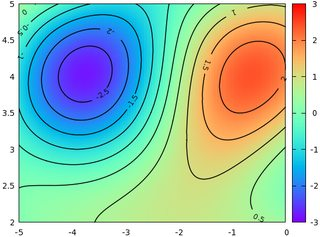
\includegraphics[width=.5\textwidth]{images/contour_plot}
\end{figure}
\end{itemize}

While the Riemann integral considers the area under a curve as made out of vertical rectangles, the Lebesgue definition considers slabs that are not necessarily just rectangles, and so it is more flexible. 



\subsection{$\S$ 1.5.1 Measurable functions}

\subsubsection{Definitions}

\begin{definition}
If $\F$ is a $\sigma$-field of subsets of $\Omega$, then $(\Omega, \F)$ is called a \textit{measurable space} and sets in $\F$ are called \textit{measurable sets}.
\label{def:measurable_space_and_measurable_sets}	
\end{definition}

We can now define measurable functions as those which preserve measurability under inverse images.
   
\begin{definition}
If $h : \Omega_1 \to \Omega_2$, $h$ is a \textit{measurable function} relative to the $\sigma$-fields $\F_j$ of subsets of $\Omega_j$, $j=1,2$, iff $h^{-1}(A) \in F_1$ for all $A \in \F_2$.  We sometimes denote measurable functions as an explicit mapping between measurable spaces: $h : (\Omega_1, \F_1) \to (\Omega_2, \F_2)$.
\label{def:measurable_function}
\end{definition}


Borel measurable functions are a special case of particular interest.  
 
\begin{definition}
A \textit{Borel measurable function} is a measurable function $h : (\Omega_1, \F_1) \to (\R^n, \B(\R^n))$ or  $h : (\Omega_1, \F_1) \to (\overline{\R}^n, \B(\overline{\R}^n))$.  
\label{def:borel_measurable_function}
\end{definition}

Note that the \textit{Borel} in Borel measurability refers to the measurable sets in the \textit{range}, not the domain.  A more precise term would be \textit{$(\F_1, \text{Borel})$-measurable}, since the condition to be a measurable function depends on both sigma-fields.  However, people do not say that.  Unless stated otherwise, we assume $\F_1 = \B$ whenever $\Omega_1$ is a Borel subset of $\R^k$ or $\overline{\R}^k$.

\subsubsection{``Computational" definitions}
In practice, to show that a function is measurable, it suffices to apply what we might call the ``computational definition of measurable functions."

\begin{claim}{\remarktitle{Computational definition of measurable functions}}
For $h : \Omega_1 \to \Omega_2$ to be measurable relative to the $\sigma$-fields $\F_j$ of subsets of $\Omega_j$, $j=1,2$, it suffices to show that $h^{-1}(B) \in \F_1$ for all $B \in \C : \sigma(\C) = \F_2$. 
\label{claim:computational_def_measurability}	
\end{claim}

\begin{proof}
We apply the ``Good Sets" strategy (see Section \ref{sec:good_sets_strategy}).  The ``base" condition is satisfied by hypothesis.  For the ``induction step", we need to show that the good sets form a $\sigma$-field.

Let us define the good sets as $\G := \set{B \in \F_2 : h^{-1}(B) \in \F_1}$.  We check the three conditions:
\begin{itemize}
\item $\Omega_2 \in \G$	? \greencheck.  True because $h^{-1}(\Omega_2) = \Omega_1 \in \F_1$ by  the fact that $\F_1$ is a $\sigma$-field.
\item $B \in \G \implies B^c \in \G$? \greencheck.  Since complements and inverse images commute (see Section \ref{sec:why_define_measurability_this_way}), we have $h^{-1}(B^c) = h^{-1}(B)^c \in \F_1$ by assumption and the fact that $\F_1$ is a $\sigma$-field, and hence closed under complements.
\item $B_1, B_2, ... \in \G \implies \cup_{i=1}^\infty B_i \in \G$? \greencheck.  Since unions and inverse images commute (see Section \ref{sec:why_define_measurability_this_way}), we have $h^{-1}(\cup_{i=1}^\infty B_i) = \cup_{i=1}^\infty h^{-1}(B_i) \in \F_1$ by assumption and the fact that $\F_1$ is a $\sigma$-field, and hence closed under countable unions.   
\end{itemize}

\end{proof}




%\begin{definition}
%Given a measurable function $h : (\Omega_1, \F_1) \to (\Omega_2, \F_2)$, sets in $\F_1$ are called the \textit{measurable sets}. 
%\label{def:measurable_sets}
%\end{definition}

\begin{remark}{\remarktitle{The computational definition of Borel measurability.}}
Thanks to Claim \ref{claim:computational_def_measurability}, to show that a function $h$ is Borel measurable, we simply need to show that $h^{-1}(B) \in \F_1$ for $B \in \C$ for any collection $\C$ that generates the Borel sets. For instance, when $h$ is real-valued, it suffices to show
\begin{itemize}
\item $h^{-1}\big((a,\infty)\big) \in \F_1$ for each $a \in \R$.
\item $h^{-1}\big([a,\infty)\big) \in \F_1$ for each $a \in \R$.
\item $h^{-1}\big((a,b)\big) \in \F_1$ for each $a,b \in \R$.
\item $h^{-1}\big([a,b]\big) \in \F_1$ for each $a,b \in \R$.
\item $h^{-1}(U) \in \F_1$ for each open set $U \subset \R$.
\item $h^{-1}(V) \in \F_1$ for each closed set $V \subset \R$.
\item etc.
\end{itemize}
For a larger list, recall Section \ref{sec:borel_sets}. 
\label{rk:computational_definition_of_Borel_measurability}
\end{remark}

\subsubsection{Examples}

\begin{example}{\remarktitle{Constant functions are measurable.}}
Consider a constant function, i.e. $h: (\Omega_1, \F_1) \to (\Omega_2, \F_2)$ such that $h(\omega) =   c$ for all $\omega \in \Omega_1$.  
\ifActive 
	\textbf{Workshop Exercise:} Show that $h$ is measurable. 
\else 
	Then $h$ is measurable, since 
	\[ h^{-1}(B) = 
	\begin{cases}
	\Omega_1, & \text{ if } c \in B\\ 
	\emptyset, & \text{ if } c \not\in B\\ 
	\end{cases}
	\]
	
	\begin{figure}[H]
	\centering
	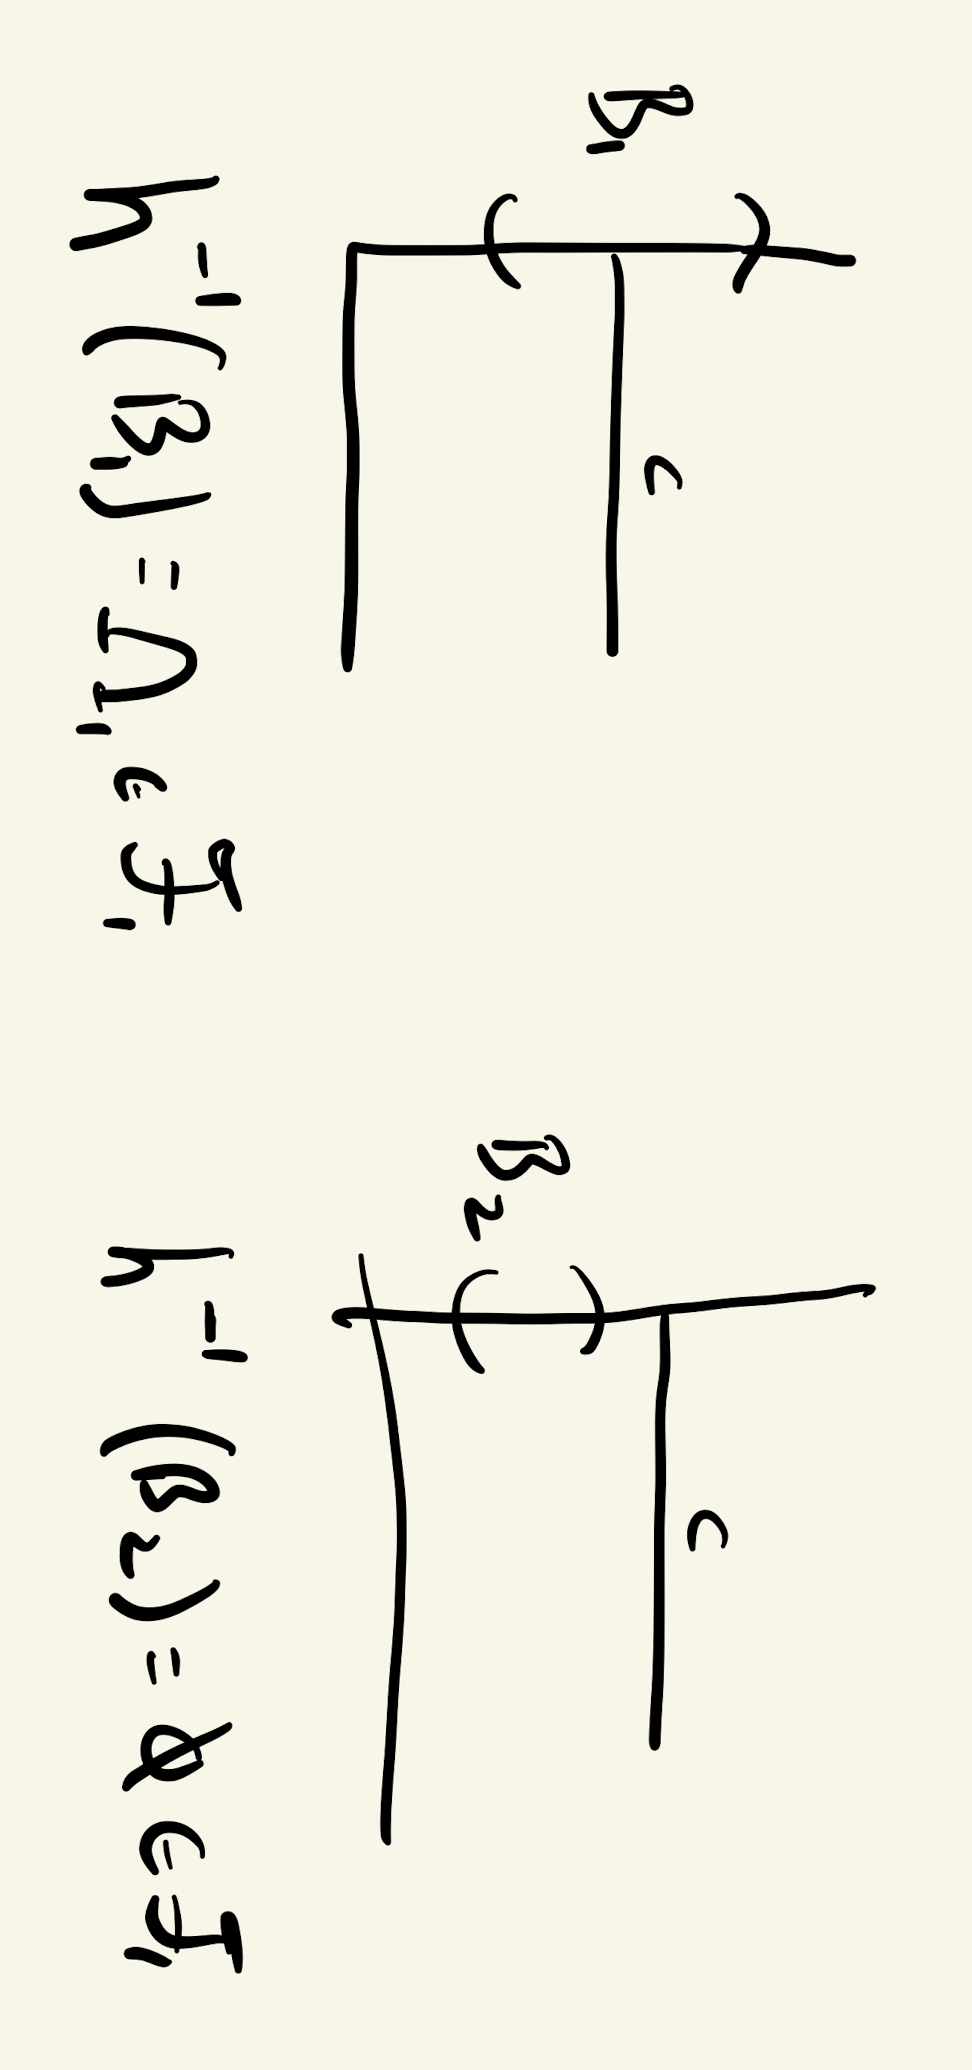
\includegraphics[angle=90, width=.5\textwidth]{images/constant_functions_are_measurable}
	\end{figure}
\fi 
\label{ex:constant_functions_are_measurable}
\end{example}

\begin{example}{\remarktitle{Any function is measurable with respect to the trivial $\sigma$-field.}}
Consider any function $h : (\Omega_1, \F_1) \to (\Omega_2, \F_2)$, where $\F_2$ is the trivial $\sigma$-field: $\F_2 = \set{\emptyset, \Omega_2}$.  Then $h$ is measurable since $h^{-1}(\emptyset) = \emptyset \in \F_1$ and  $h^{-1}(\Omega_2) = \Omega_1 \in \F_1$
\label{ex:any_function_is_measurable_with_respect_to_trivial_sigma_field}	
\end{example}

\begin{example}{\remarktitle{Indicators of Borel sets are Borel measurable.}}
Let $A$ be a Borel subset of $\R$,\footnote{Recall Section \ref{sec:borel_sets}.  For instance, we might take $A$ to be an open interval, or a disjoint union of open intervals, or the Cantor set.} and let $I_A : \R \to \R$ be the indicator of $A$; that is $I_A(x)=1$ for $x \in A$ and $0$ for $x \not\in A$. Then $I_A$ is Borel measurable, since for all $B \in \B(\R)$, we have
\[ I_A^{-1}(B) = 
\begin{cases}
\R, & \text{ if } 0,1 \in B\\ 
A, & \text{ if } 1 \in B, 0 \not\in B \\
A^c, & \text{ if } 0 \in B, 1 \not\in B \\	
\emptyset, & \text{ if } 0,1 \not\in B\\ 
\end{cases}
\]

\begin{figure}[H]
\centering
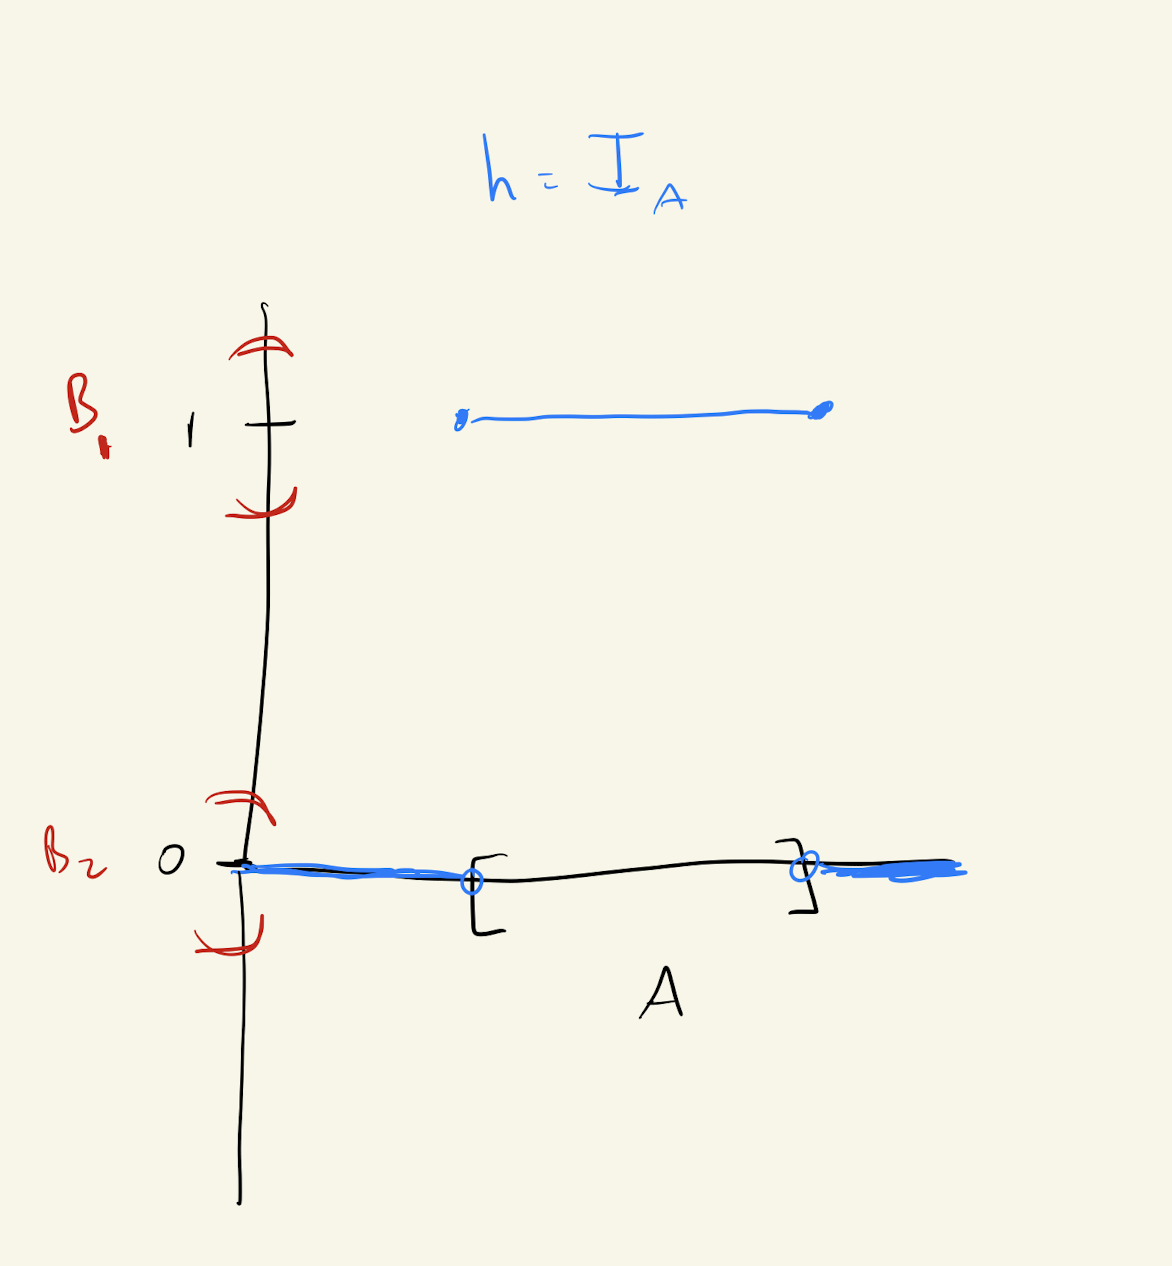
\includegraphics[width=.4\textwidth]{images/indicator_of_borel_set}	
\end{figure}

\end{example}

\begin{example}{\remarktitle{Indicators of non-Borel sets are not Borel measurable - but they may still be measurable.}}
Let $A$ be a subset of $\R$ that is not Borel (e.g., $A$ could be the non-Borel set described in Section \ref{sec:set_that_is_not_Lebesgue_measurable}), and let $I_A : \R \to \R$ be the indicator of $A$.   Then $I_A$ is \textit{not} Borel measurable.  

However, $I_A$  \textit{is} measurable with respect to the trivial sigma-field; that is, if we take the mapping to be $I_A : (\R, \B(\R)) \to (\R, \F_2)$, where $F_2 := \set{\emptyset, \R}$.  See Example \ref{ex:any_function_is_measurable_with_respect_to_trivial_sigma_field}.
\label{ex:indicators_of_non_borel_sets_are_not_borel_measurable}
\end{example}

\begin{example}{\remarktitle{Continuous functions are Borel measurable}}. Let $h : \R^k \to \R^n$ be continuous.  Since $h$ is continuous, the inverse image of any open set is open. Hence $h$ is Borel measurable by the computational definition of Borel measurability -- see Remark \ref{rk:computational_definition_of_Borel_measurability}.
\end{example}

\subsubsection{Why define measurability this way?} \label{sec:why_define_measurability_this_way}

Measurable functions do \textit{not} preserve measurability in \textit{both} directions. That is, if $h : (\Omega_1, \F_1) \to (\Omega_2, \F_2)$ is a measurable function, it is not necessarily true that $h(A) \in \F_2$ for all $A \in \F_1$.  For a counterexample, we take $\F_2 = \set{\emptyset, \Omega_2}$, recalling Example \ref{ex:any_function_is_measurable_with_respect_to_trivial_sigma_field}.   Then any $h$ is measurable.  But if there is $A \in F_1$ such that $h(A)$ is a nonempty proper subset of $\Omega_2$, then it is not a measurable set ($h(A) \not\in \F_2$). 

So why is measurability defined by preserving measurability over \textit{inverse} images, rather than in terms of direct images?  In measure theory, inverse images are much nicer objects than direct images.  This is because basic set operations are preserved by inverse images, but in general not by images.  

In particular, for any function $f$
\begin{alphabate}
\item Inverse images and complements commute: $f^{-1}(B^c) = \big(f^{-1}(B)\big)^c$	

\textit{Proof.} $ \big(f^{-1}(B)\big)^c := \set{x : x \not\in f^{-1}(B) } = \set{x : f(x) \not\in B } = \set{x: f(x) \in B^c} = \set{x: x \in f^{-1}(B^c)} := f^{-1}(B^c).$

\begin{figure}[H]
\centering
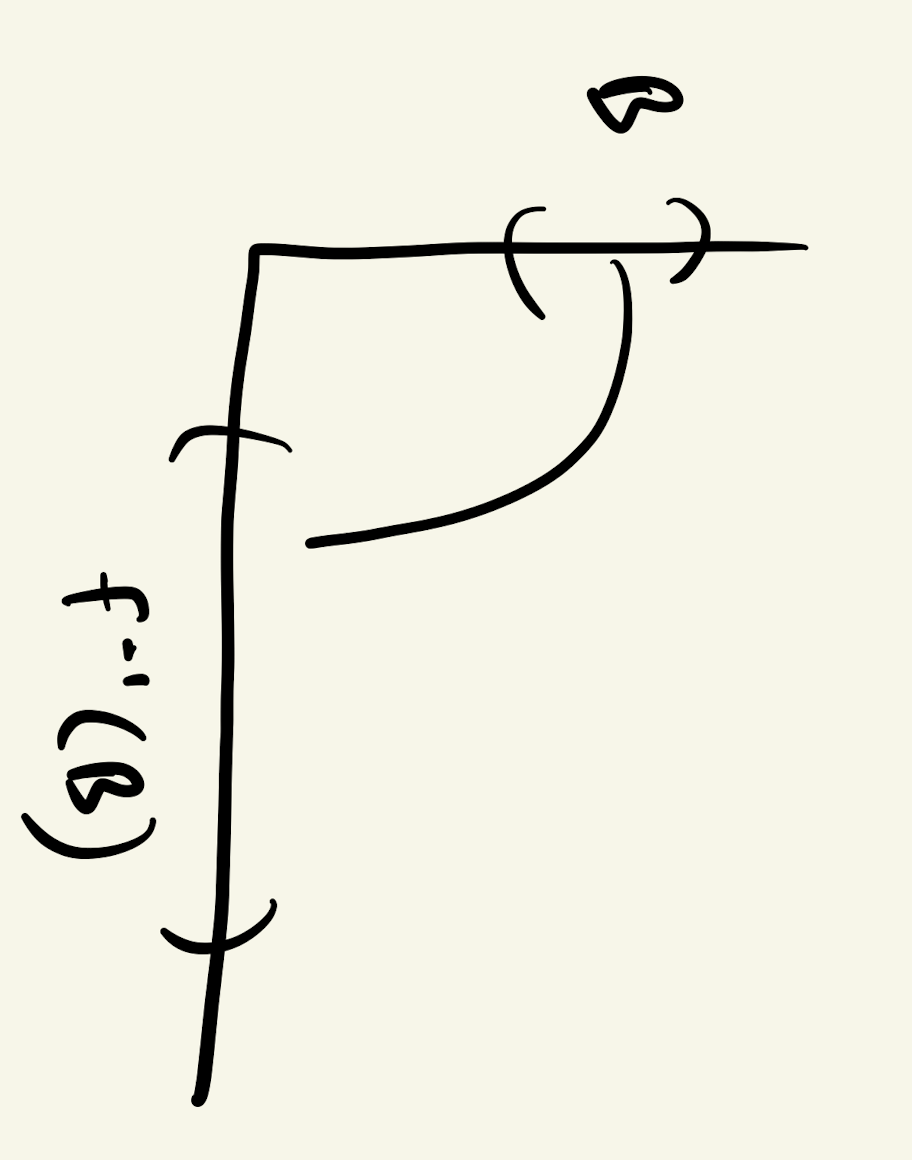
\includegraphics[angle=90, width=.25\textwidth]{images/inverse_images_and_complements_commute}	
\end{figure}


\item Inverse images and unions commute: $f^{-1}(\cup_i B_i) = \cup_i \big(f^{-1}(B_i)\big)$
\item Inverse images and intersections commute: $f^{-1}(\cap_i B_i) = \cap_i \big(f^{-1}(B_i)\big)$	
\end{alphabate}

However, 
\begin{itemize}
\item[d)] Direct images and complements do not in general commute: $f(A^c) \neq \big(f(A)\big)^c$	

\ifActive 
	\textbf{Workshop Exercise:} Prove this.
\else 
	\textit{Proof.} Let $f : \Omega \to \R$ be the constant function, i.e. $f(\omega) = c$ for some $c \in \R$ for all $\omega \in \Omega$.  Let $A$ be a non-empty proper subset of $\Omega$.  Then $f(A) = c$ and $f(A^c) = c$.  So $\R \setminus c = \big(f(A)\big)^c \neq  f(A^c) = c$.
	
	\begin{figure}[H]
	\centering
	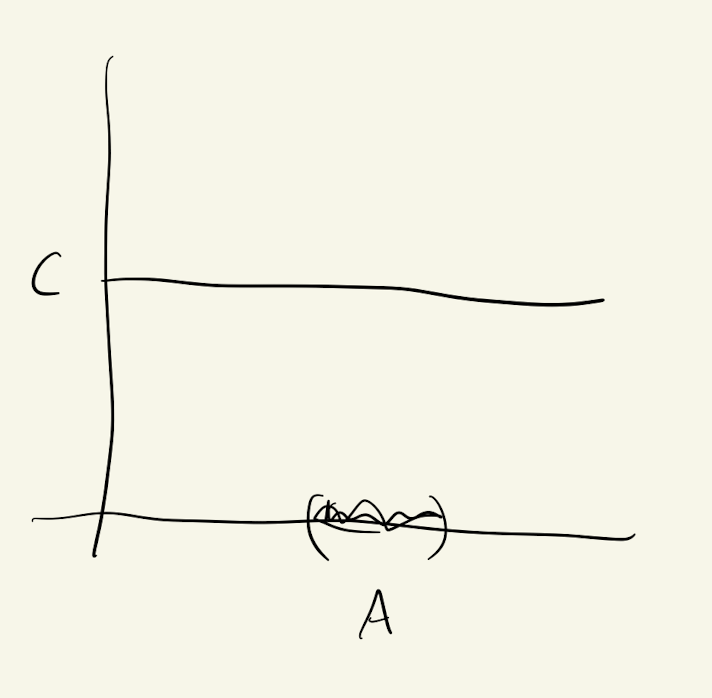
\includegraphics[width=.25\textwidth]{images/direct_images_and_complements}	
	\end{figure}
\fi 

\item[e)] Direct images and intersections do not in general commute: $f(\cap_i A_i) \neq \cap_i \big(f(A_i)\big)$	
\end{itemize}

Recall in Section \ref{sec:intuition_on_Lebesgue_integration} that Lebesgue and Riemann integration are distinguished in terms of whether they partition the range or domain of the function.  My speculation is that the nice interplay of basic set operations and inverse images (but not direct images) at least partially explains why Lebesgue's approach has been more successful than Riemann's approach (in the sense of better limit theorems, better handling of non-Euclidean spaces, etc.).

\subsubsection{Closure properties} \label{sec:closure_properties_of_measurable_functions}

\begin{proposition}
If $h_1, h_2 : (\Omega, \F) \to (\overline{\R}, \B(\overline{\R}))$ are Borel measurable, then so are $h_1 + h_2$ and $h_1 h_2$.  
\label{prop:borel_measurability_closed_under_multiplication_and_addition}
\end{proposition}

\begin{proof}
See \cite{folland1999real} Proposition 2.6.
\end{proof}

\begin{proposition}
If $\set{h_n}$ is a sequence of $\overline{\R}$-valued Borel measurable functions on $(\Omega, \F)$, then the functions
\begin{align*}
\sup_n h_n(\omega), & \quad \quad \limsup_{n \to \infty} h_n(\omega) \\
\inf_n h_n(\omega), & \quad \quad  \liminf_{n \to \infty} h_n(\omega) \\	
\end{align*}
are all measurable. Thus, if $h(\omega) = \lim_{n \to \infty} h_n(\omega)$ exists for all $\omega \in \Omega$, then $h$ is measurable.
\label{prop:borel_measurability_closed_under_inf_sup_liminf_limsup}
\end{proposition}

\begin{proof}
See \cite{folland1999real} Proposition 2.7.
\end{proof}

\begin{proposition} 
A composition of Borel measurable functions is measurable.
\label{prop:a_composition_of_Borel_measurable_functions_is_measurable}
\end{proposition}

\begin{proof}
See \cite{ash2000probability} Lemma 1.5.7.
\end{proof}


Below we see that Borel measurability of a multivariate function is equivalent to the Borel measurability of all the component functions.

\begin{proposition}
\cite[Thm.~1.5.8]{ash2000probability}.   Let $h : \Omega \to \overline{\R}^n$.  So $h=(h_1(\omega), \hdots, h_n(\omega))$.  Then $h$ is Borel measurable iff $h_i$ is Borel measurable for all $i=1,\hdots n$.  
\label{prop:multivariate_function_is_Borel_measurbale_iff_component_functions_are_Borel_measurable}
\end{proposition}

\begin{proof}
First, some notation.  Let $p_i : \overline{\R}^n \to \overline{\R}$ be the projection map taking $(x_1,\hdots, x_n)$ to $x_i$.   Then each component function can be written as $h_i = p_i \circ h$.

Now we prove each direction
\begin{itemize}
\item $\boxed{\implies}$.  Let $h$ be Borel measurable. We need to show that
\[ h_i^{-1}(B) \in \B(\overline{\R}), \quad \forall B \in \B(\overline{\R}). \]
By the computational def. of measurable functions (see Remark~\ref{rk:computational_definition_of_Borel_measurability}), it suffices to show that 
\[ h_i^{-1}(I) \in \B(\overline{\R}), \quad \forall I = [a,b] \subset \overline{\R}.\]
So note that each $p_i$ is Borel measurable, since 
 \[ p_i^{-1} \set{x_i \in \overline{\R} : a_i \leq x_i \leq b_i} = \set{x \in \overline{\R}^n : a_i \leq x_i \leq b_i,  -\infty \leq x_j \leq \infty, \quad j \neq i }\]
 which is an interval of $\overline{\R}^n$.  So $h_i = p_i \circ h$ is the composition of measurable functions, which is measurable by Proposition~\ref{prop:a_composition_of_Borel_measurable_functions_is_measurable}.

\item $\boxed{\impliedby}$. Let each $h_i$ be Borel measurable.   Again using Remark~\ref{rk:computational_definition_of_Borel_measurability}, we have
\begin{align*}
h^{-1} \set{x \in \overline{\R}^n : a \leq x \leq b} &= \bigcap_{i=1}^n \set{\omega \in \Omega : a_i \leq h_i(\omega) \leq b_i} \explaintermbrace{by hypoth.}{\in \F}.
\end{align*}
  
\end{itemize}
 	
\end{proof}

%{rk:computational_definition_of_Borel_measurability}

\subsection{$\S$ 1.5.2-1.5.3 Integrating  Borel measurable functions}

In this section, we define integral of a Borel measurable function $h : (\Omega, \F) \to (\overline{\R}, \B(\overline{\R}))$ against arbitrary measure $\mu$.  The integral can be written as:
\[ \ds\int_{\Omega} h \wrt{\mu}, \quad \quad \ds\int_{\Omega} h(\omega) \wrt{\mu(\omega)}, \quad \text{ or } \quad \ds\int_{\Omega} h(\omega) \mu(d \, \omega) \]
 
 We proceed in three steps: first, we consider where $h$ is simple, then we consider $h$ non-negative, then we consider $h$ arbitrary. 



\subsubsection{Integrals of simple functions}

\paragraph{Definition of simple functions} 

\begin{definition}
Let $(\Omega, \F)$ be a measurable space, fixed throughout the discussion.  If $h : \Omega \to \overline{\R}$, $h$ is said to be \textit{simple} iff $h$ is measurable and takes on only finitely many distinct values.  That is, $h$ is simple iff it can be written $h = \sum_{i=1}^r y_i I_{A_i}$ where the $A_i$ are disjoint sets in $\F$ and $I_{A_i}$ is the indicator of $A_i$; the $y_i$ need not be distinct. 
\label{def:simple_function}	
\end{definition}

\begin{remark}{\remarktitle{Simple functions generalize step functions}}
A special case of simple functions are the step functions used in Riemann integration. 


For $a,b \in \overline{\R}$ with $a<b$, $f : [a,b] \to \R$ is a \textit{step function} if there exists a partition $a = x_0 < x_1 < ... < x_n = b$ and constants $y_1, ..., y_n \in \R$ such that $f(x)=y_i$ for all $y \in (x_{i-1},x_i)$ and each $i=1,...,n$.  Then $f$ is equal to the following simple function:
\[ y_i I_{(x_{i-1}, x_i)} + f(x_i) I_{\set{x_i}}\]

Note that in this case, the sets $A_i$ take on a specific form, as open intervals or one of finitely many singletons.  In general, simple functions allow more general $A_i$. 

%Some observations:
%\begin{itemize}
%\item In this case, the sets $A_i$ take on a specific form, as open intervals or singletons.  In general, simple functions allow more general $A_i$. 
%\item Simple functions do not require that the domain is totally ordered.  
%\end{itemize}
\label{rk:simple_functions_generalize_step_functions}
\end{remark}

\begin{remark}
Note that the indicator function for a non-Borel set (see Example \ref{ex:indicators_of_non_borel_sets_are_not_borel_measurable}) is \textit{not} a simple function, even though it only takes on values 0 and 1. 
%Note that the term \textit{simple} in simple function refers to properties of \textit{both} the domain and range. So for instance, the indicator function for a non-Borel set (see Example \ref{ex:indicators_of_non_borel_sets_are_not_borel_measurable}) is \textit{not} a simple function, even though it only takes on values 0 and 1.  
\end{remark}

\paragraph{Definition of the integral of simple functions}

\begin{definition}
Let $h$ be simple, say $h = \sum_{i=1}^r y_i I_{A_i}$ where the $A_i$ are disjoint sets in $\F$.  Then
\begin{align*}
\ds\int_{\Omega} h \wrt{\mu} := \ds\sum_{i=1}^r y_i \; \mu(A_i).
\labelit \label{eqn:integral_of_simple_function}	
\end{align*}
 \label{def:integral_of_simple_function}
\end{definition}

The integral of a simple function can also be expressed as 
\[\ds\int_{\Omega} h \wrt{\mu} := \ds\sum_{i=1}^r y_i \; \mu \bigg( h^{-1}(y_i) \bigg) \]

\begin{figure}[H]
\centering 
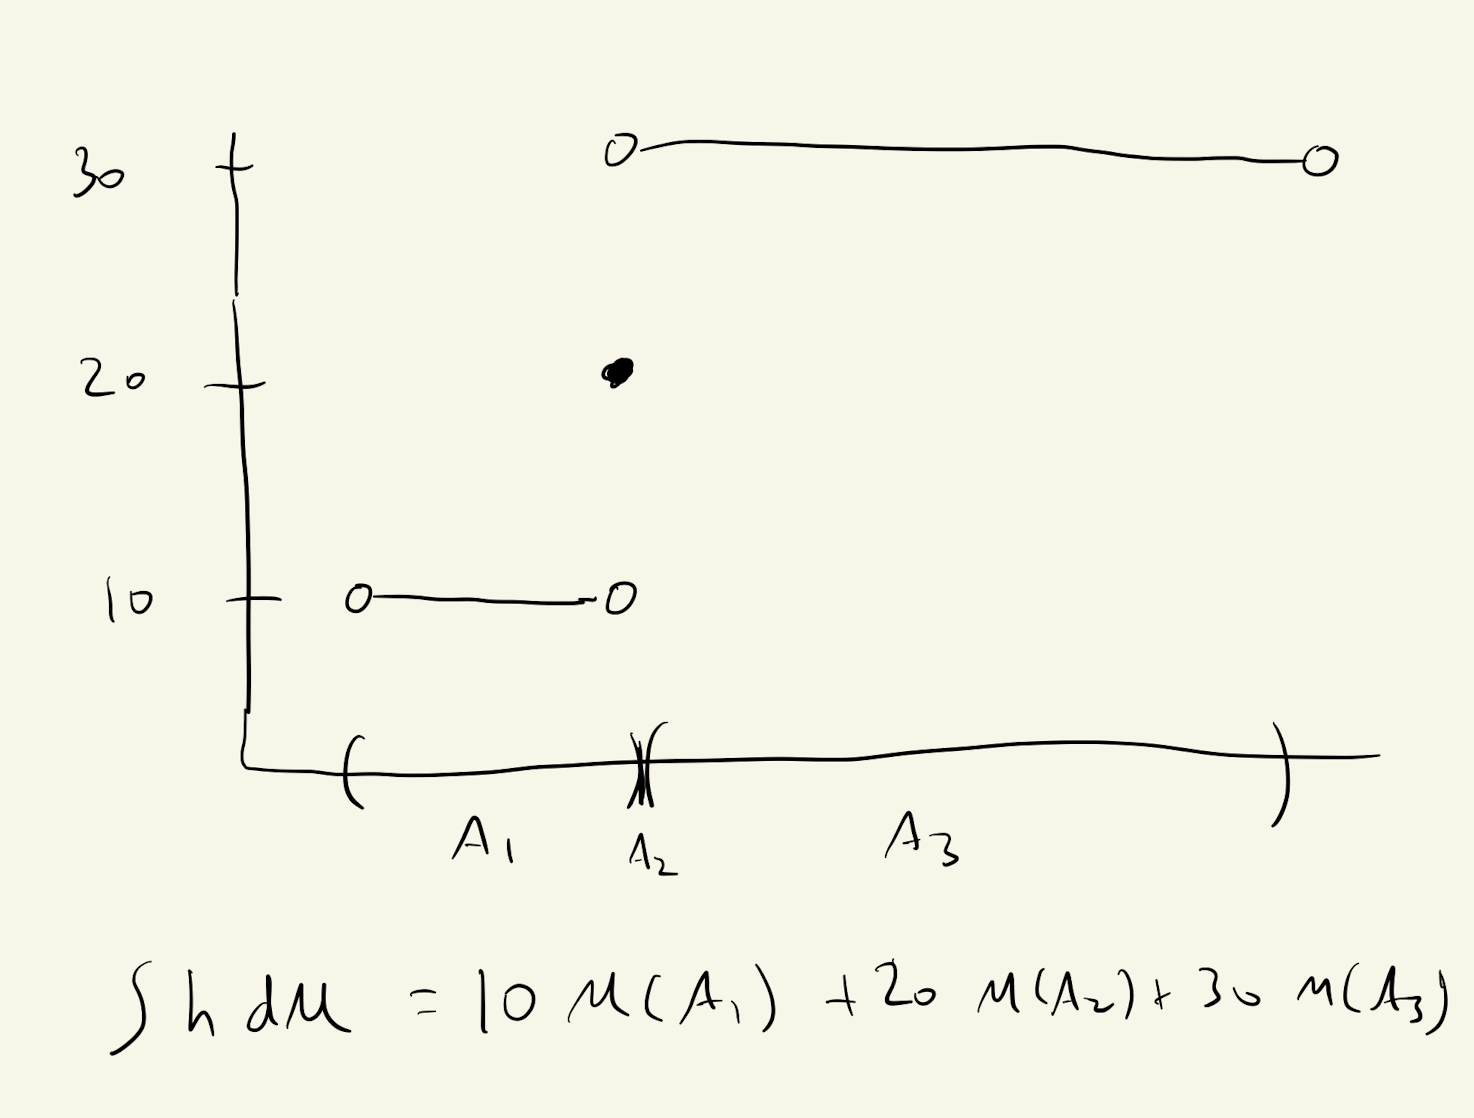
\includegraphics[width=.5\textwidth]{images/integral_of_simple_function}	
\caption{The Lebesgue integral of a simple function. {\scriptsize (In this case, the simple function is also a step function.)}}
\end{figure}

\begin{remark}{\remarktitle{When does the integral of a simple function exist}}
The integral of a simple function exists whenever $\infty$ and  $-\infty$ do not both appear in the sum.  So in particular, the integral for $h$ does not exist when
\begin{itemize}
\item The finite values it takes on $\set{y_i}_{i=1}^r$ include 	$\infty$ and $-\infty$ on sets that are not of measure zero.
\begin{figure}[H]
\centering
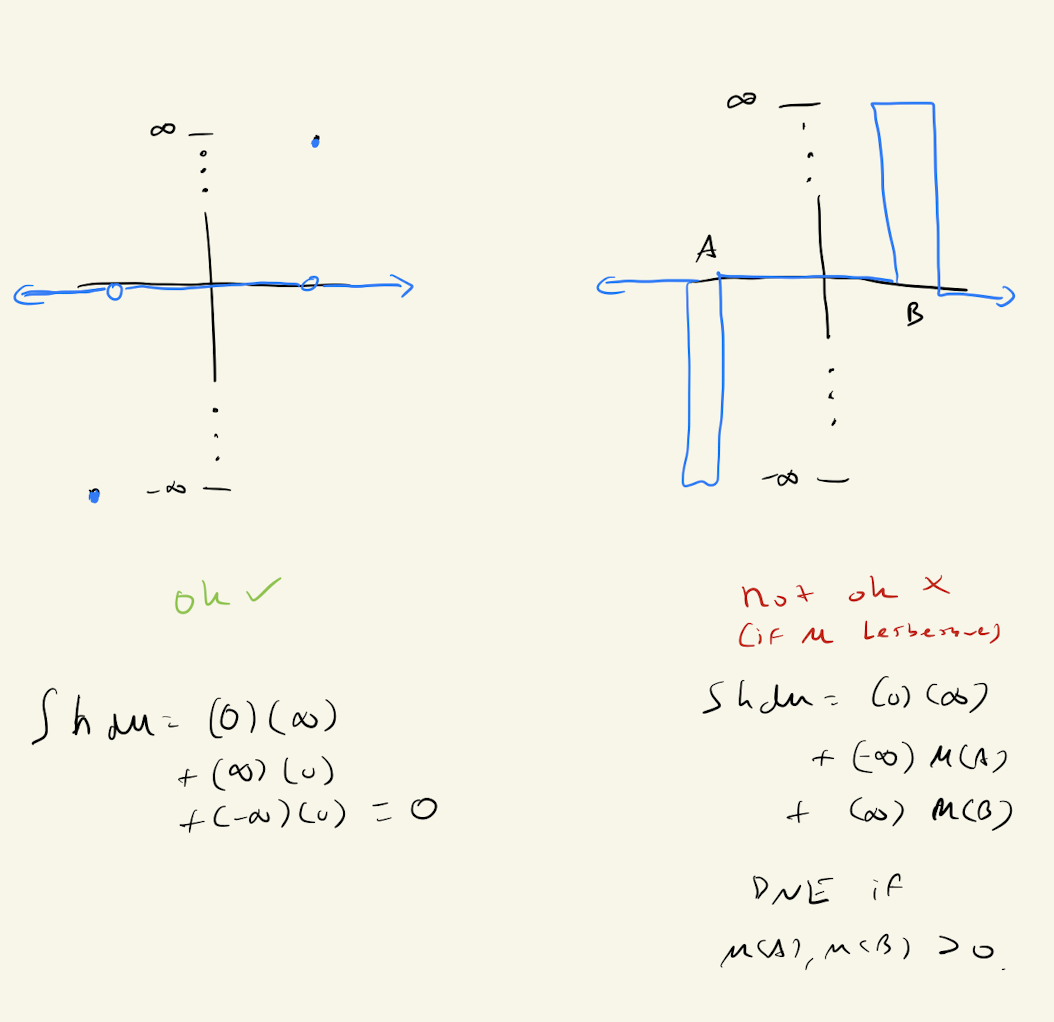
\includegraphics[width=.5\textwidth]{images/when_does_integral_of_simple_function_exist_part_1}
\end{figure}

\item It takes on values of opposite signs on two sets of infinite measure.
\begin{figure}[H]
\centering
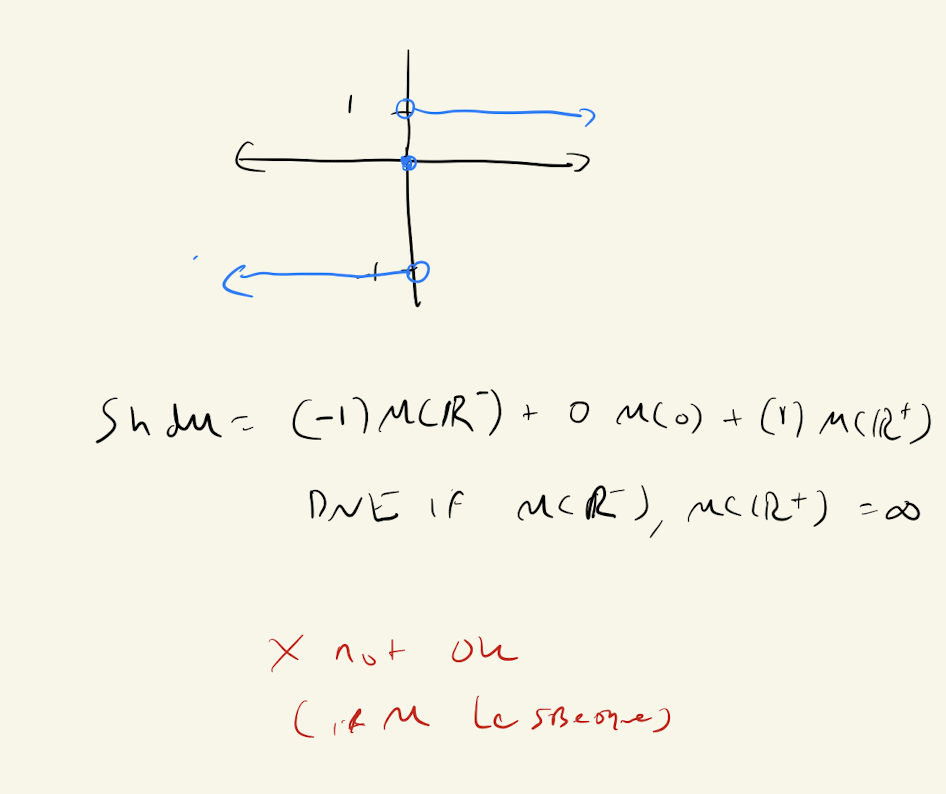
\includegraphics[width=.5\textwidth]{images/when_does_integral_of_simple_function_exist_part_2}
\end{figure}
\end{itemize}
 
\label{rk:when_does_integral_of_simple_function_exist}
\end{remark}

\begin{remark}{\remarktitle{Integrating simple functions over arbitrary measurable subsets}}
For any $A \in \F$ and simple function $s$, we define 
\[ \ds\int_A s \wrt{\mu} := \ds\int_\Omega s \, \indicate{A} \wrt{\mu}  \]

This definition is possible because whenever $s$ is a simple function, then so is $s \indicate{A}$ for any measurable set $A$.   Indeed, if we express $s = \sum_{i=1}^r y_i \indicate{{B_i}}$, then $s \indicate{A} = \sum_{i=1}^r y_i \indicate{A} \indicate{B_i} = \sum_{i=1}^r y_i \indicate{A \cap B_i}$, and each $A \cap B_i \in \F$.  
\label{rk:integrating_simple_functions_over_arbitrary_measurable_subsets}
 \end{remark}
 
\paragraph{Comparison to Riemann integration}

\begin{example}{\remarktitle{Integrating a step function}}
Let $h$ be a step function, as defined in Remark \ref{rk:simple_functions_generalize_step_functions}.   So  $a = x_0 < x_1 < ... < x_n = b$ is a partition of $\Omega := \text{dom}(h)$, and $h$ takes on values $y_i$ on $(x_{i-1},x_i)$ for $i=1,...,n$.  Then 
\begin{align*}
\ds\int_{\Omega} h \wrt{\mu} &= \ds\sum_{i=1}^n y_i \; \mu(x_{i-1},x_i) + \ds\sum_{i=1}^n f(x_i) \mu\set{x_i} \\
& \stackreltext{(if $\mu$ is Lebesgue measure)}{=} \; \ds\sum_{i=1}^n y_i \; (x_i - x_{i-1}) + \cancelto{0}{\ds\sum_{i=1}^n f(x_i) \mu\set{x_i}}
\end{align*}

So the Lebesgue integral of the step function agrees with the Riemann integral when $\mu$ is Lebesgue measure (although not for general measure).
\end{example}

Now we integrate a simple function that is not a step function -- in fact, a simple function for which there is not a Riemann integral. 

\begin{example}{\remarktitle{Integrating the Dirichlet function}}
Let $h$ be the Dirichlet function; that is $h = I_{\Q} : \R \to \R$ is the indicator of the rationals.  Let us integrate $h$ against Lebesgue measure $\mu$. 
%
\ifActive 
	\textbf{Workshop Exercise:} Derive the integral. 
\else 
	\begin{align*}
	\ds\int_{\Omega} h \wrt{\mu} &= 1 \; \mu(\Q) + 0 \; \mu(\R - \Q) && \tinytext{def. integral of simple function} \\
	 &= 1 \; \mu(\Q) && \tinytext{arithmetic of $\overline{\R}$: \; $0 \cdot x = 0$ for $x \in \overline{\R}$} \\
	 	&= 1 \; \mu(\bigcupdot_{q \in \Q} \set{q}) && \tinytext{rewrite $\Q$} \\
	&= 1 \; \ds\sum_{q \in \Q} \mu(\set{q}) && \tinytext{countable additivity, $\Q$ is countable} \\
	& \stackrel{1}{=} 1 \ds\sum_{q \in \Q} 0 && \tinytext{Proposition \ref{prop:properties_of_LS_measures}} \\
	&= 0.  
	\end{align*}
	Note Equation 1 holds for any Lebesgue-Stieljes measure with a continuous distribution function (see Remark \ref{rk:continuity_at_a_point_iffi_measure_zero_at_a_point}).  However, other measures may yield other results.
\fi 
\label{ex:integrating_the_dirichlet_function}
\end{example}

Now we show that the Dirichlet function does not have a Riemann integral. 

\begin{remark}{\remarktitle{The Dirichlet function does not have a Riemann integral.}}	
Let $h$ be the Dirichlet function; that is $h = I_{\Q} : \R \to \R$ is the indicator of the rationals.  Fix $[a,b] \subset \R$, and let $f=h |_{[a,b]}$; that is $f : [a,b] \to \R$ is the Dirichlet function restricted to $[a,b]$.  

We consider an arbitrary \textit{partition} $P$ of $[a,b]$ into a collection of $n$ subintervals via a finite sequence $P=\set{x_i}_{i=0}^n$ such that $a=x_0 < x_1 < ... < x_n = b$.  Now by Proposition \ref{prop:Riemann_integrable_iff_oscillation_goes_to_zero_as_partition_gets_finer}, a function on $[a,b]$ is Riemann integrable iff $\text{Osc}(f,P) \to 0$ as the maximum interval length of a partition $P$ goes to 0.\footnote{For a refresher on how these terms are defined, see Section \ref{sec:some_info_relevant_to_Riemann_integrals}.}  But for any partition $P$, any subinterval $(x_{k-1}, x_k)$ will contain at least one rational number and at least one irrational number, and so
\begin{align*}
S^+(f,P) &= \ds\sum_{k=1}^n 1 \cdot (x_k - x_{k-1}) = b-a \\	
S^-(f,P) &= \ds\sum_{k=1}^n 0 \cdot (x_k - x_{k-1}) = 0\\
\end{align*}
Thus $\text{Osc}(f,P) = b-a$ for all partitions $P$. In particular $\text{Osc}(f,P) \not\to 0$ 	as the maximum interval length of a partition $P$ goes to 0.\footnote{To be more explicit, the condition of Proposition \ref{prop:Riemann_integrable_iff_oscillation_goes_to_zero_as_partition_gets_finer} is that $\forall \epsilon > 0, \;\exists \delta >0  : \forall P  \text{ where the maximum interval length of } P < \delta, \; \text{Osc}(f,P) < \epsilon$. But since $\text{Osc}(f,P) = b-a$ for all partitions $P$, the condition is contradicted: $\exists \epsilon = \frac{b-a}{2} >0 : \forall P, \text{Osc}(f,P) > \epsilon.$}  Thus $f$ is not Riemann integrable. 

The Riemann integral of $h: \R \to \R$ would be an improper integral defined as the limiting value of the Riemann integrals $h|_{[a,b]}$ as $a \to -\infty, b \to \infty$.  But since the proper Riemann integrals for $h|_{[a,b]}$ don't exist, neither does the improper Riemann integral for $h$. 
\label{rk:dirichlet_function_is_not_Riemann_integrable}
\end{remark}

%Recall that a proper Riemann integral $\int_{a}^b f(x) \, dx$, when it exists,  is defined only for real-valued functions  $f$ whose domain is a compact space $[a,b] \subset \R$.  Recall also that an improper Riemann integral is  defined for functions $h: \R \to \R$ as the limiting value of proper Riemann integrals.  

% Commenting this out because we haven't defined almost everywhere yet.

%\begin{remark}{\remarktitle{The Dirichlet function does not have a Riemann integral}} A function on $[a,b]$ is Riemann integrable if and only if it is bounded and continuous almost everywhere.  However, the Dirichlet function $f$ is continuous nowhere.  For every irrational number $x$, there is a sequence of rational numbers $\{r_n\}$ that converges to it. We have:
%$$
%\lim_{n\to\infty} f(r_n) = 1 \ne 0 = f(x)
%$$
%
%Thus, $f$ isn't continuous at irrational numbers. Rational numbers can be handled similarly.
%	
%\label{rk:dirichlet_function_has_no_Riemann_integral}
%\end{remark}
%\end{document}
%
%Example \ref{ex:integrating_the_dirichlet_function} shows how Lebesgue integration can handle functions not handled by Riemann integration.  As noted in Remark \ref{rk:{rk:dirichlet_function_has_no_Riemann_integral}, a function on $[a,b]$ is Riemann integrable if and only if it is bounded and continuous almost everywhere.  Lebesgue integration can handle functions that do not meet these criteria.

\paragraphnewline{Properties of integrals of simple functions} 

In this section, for now, we only provide properties that come up in our exposition.  For other useful properties, see Proposition 2.13 of \cite{folland1999real}.


\begin{proposition} 
Let $g$ and $h$  be simple functions.  Then 
\begin{alphabate}
\item (monotonicity) If $g \leq h$ then $\ds\int g \wrt{\mu} \leq \ds\int h \wrt{\mu}$.
\item (additivity) $\ds\int (g + h) \wrt{\mu} = \ds\int g \wrt{\mu} + \ds\int h \wrt{\mu}$ .
\item (scalar multiple property) $\ds\int c \, g \wrt{\mu} = c \ds\int g \wrt{\mu}$.
\end{alphabate}
\label{prop:properties_of_integrals_of_simple_functions}
\end{proposition}

\begin{proof}


\begin{alphabate}
\item 
\ifActive 
	\textbf{Workshop exercise:} Prove that the monotonicity property holds for integrals of simple functions.
\else 
	By definition of simple functions, we write \[g = \ds\sum_{i=1}^r x_i I_{A_i} ,\quad \quad h = \ds\sum_{j=1}^s y_j I_{B_j}  \]	
	But if we use a common (finer) partition of $\Omega$ into sets $\set{A_i \cap B_j}$, we can write
	\begin{align*}
	g = \ds\sum_{i=1}^r \ds\sum_{j=1}^s x_i I_{A_i \cap B_j} ,\quad \quad h = \ds\sum_{i=1}^r \ds\sum_{j=1}^s y_j I_{A_i \cap B_j}  
	\labelit \label{eqn:two_simple_functions_with_common_partition}
	\end{align*}
	
	where by assumption, $x_i \leq y_j$ on each $A_i \cap B_j$.	
		
	So 
	\begin{align*}
	\ds\int g \wrt{\mu}  = \ds\sum_{i=1}^r \ds\sum_{j=1}^s x_i \, \mu(A_i \cap B_j)  \leq \ds\sum_{i=1}^r \ds\sum_{j=1}^s y_i \, \mu(A_i \cap B_j) = \ds\int h \wrt{\mu}.
	\end{align*}
\fi 
\item We sum the two forms in \eqref{eqn:two_simple_functions_with_common_partition} and apply the definition of integral of simple functions to obtain
\begin{align*}
\ds\int (g+h) \wrt{\mu} = \ds\sum_{i=1}^r \ds\sum_{j=1}^s (x_i + y_j) \, \mu(A_i \cap B_j)
\labelit \label{eqn:intermediate_result_addivity_of_simple_functions}
\end{align*}

But since we have 
\[A_i =\bigcupdot_j (A_i \cap B_j), \quad  B_j =\bigcupdot_i (A_i \cap B_j)\]
Then by finite additivity
\[\mu(A_i) =\sum_{j=1}^s \mu(A_i \cap B_j), \quad  \mu(B_j) =\sum_{i=1}^r \mu(A_i \cap B_j)\]
And so
\begin{align*}
\ds\int g \wrt{\mu} &= \ds\sum_{i=1}^r x_i \mu(A_i) = \ds\sum_{i=1}^r x_i \bigg(\sum_{j=1}^s \mu(A_i \cap B_j)\bigg) \\	
\ds\int h \wrt{\mu} &= \ds\sum_{j=1}^s y_i \mu(B_i) = \ds\sum_{j=1}^s y_i \bigg(\sum_{i=1}^r \mu(A_i \cap B_j)\bigg) \\	
\end{align*}
and summing these together yields \eqref{eqn:intermediate_result_addivity_of_simple_functions}.
\item This follows immediately from the distributive property.
\[ c \ds\int g \wrt{\mu} = c \ds\sum_{i=1}^r x_i \mu(A_i) =  \ds\sum_{i=1}^r c \, x_i \mu(A_i) = \ds\int cg \wrt{\mu} \]
\end{alphabate}

\end{proof}

\begin{proposition}
Let $s$ be a non-negative simple function. Then 
\[ A \mapsto \ds\int_A s \wrt{\mu} \]
is a measure on $\F$.
\label{prop:the_integral_of_a_simple_function_over_a_set_is_one_way_to_measure_that_set} 
\end{proposition}

\begin{proof}
Weshow  countable additivity.\footnote{Non-negativity is clear from the definition.  See Remark \ref{rk:integrating_simple_functions_over_arbitrary_measurable_subsets}.}  So let $A = \bigcupdot_{i=1}^\infty A_i$.   Writing the simple function as $s = \sum_{j=1}^r y_j \indicate{B_j}$, we obtain

\begin{align*}
\ds\int_A s \wrt{\mu} &= \ds\sum_{j=1}^r y_j \, \mu(B_j \cap A) && \tinytext{Integrals of simple functions over subsets (see Remark \ref{rk:integrating_simple_functions_over_arbitrary_measurable_subsets})} \\
&= \ds\sum_{j=1}^r \ds\sum_{i=1}^\infty y_i \, \mu(B_j \cap A_i) && \tinytext{countable additivity -- note $\bigg(B_j \cap \bigcupdot_{i=1}^\infty A_i \bigg) = \bigcupdot_{i=1}^\infty (B_j \cap A_i)$} \\
&= \ds\sum_{i=1}^\infty  \ds\sum_{j=1}^r y_i \, \mu(B_j \cap A_i) && \tinytext{sum of limit is limit of sum} \\
&= \ds\sum_{i=1}^\infty \ds\int_{A_i} s \wrt{\mu} &&  \tinytext{Remark \ref{rk:integrating_simple_functions_over_arbitrary_measurable_subsets}} 
\end{align*}
\end{proof}

\begin{remark}
Proposition \ref{prop:the_integral_of_a_simple_function_over_a_set_is_one_way_to_measure_that_set} says that we can measure a set by integrating a simple function over it.  Given some initial measure for $A$, we can get a new measure by breaking $A$ into finitely many (measurable) pieces and giving different weights to the measures of the different pieces.

\begin{figure}[H]
\centering
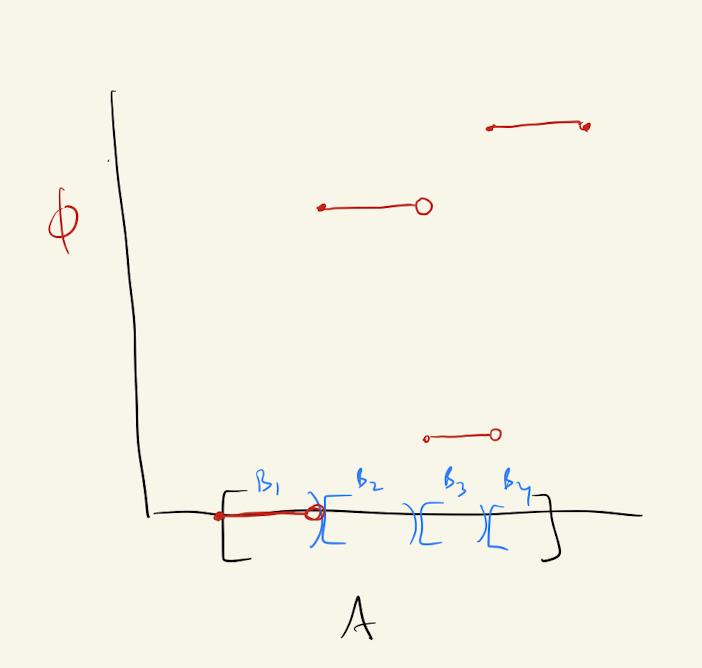
\includegraphics[width=.5\textwidth]{images/integrals_of_simple_functions_induce_new_measures}
\end{figure}
\end{remark}

\begin{remark}{\remarktitle{Continuity of measure applied to measures given by integrals of simple functions over sets}}
Recall (Theorem \ref{thm:continuity_of_countably_additive_set_functions}) that measure satisfies continuity from below: if $A_n$ are measurable and $A_n \uparrow A$, then $\lim_{n \to \infty} \mu(A_n) = \mu(A)$.    Combining this with Proposition \ref{prop:the_integral_of_a_simple_function_over_a_set_is_one_way_to_measure_that_set}, we have that if $A_n$ are measurable and $A_n \uparrow A$,
\[ \ds\lim_{n \to \infty} \ds\int_{A_n} s \wrt{\mu} =  \ds\int_A s \wrt{\mu} \]
for any simple function $s$.  
\label{rk:continuity_of_measure_applied_to_measures_given_by_integrals_of_simple_functions_over_sets}
\end{remark}



\subsubsection{Integrals of non-negative Borel measurable functions}

\paragraph{Definition of integral of non-negative Borel measurable functions}

\begin{definition}
If $h$ is non-negative Borel measurable, we define 

\begin{align*}
\ds\int_{\Omega} h \wrt{\mu} = \sup \bigg\{ \ds\int_{\Omega} s \wrt{\mu} : s \quad \text{simple,} \quad 0 \leq s \leq h  \bigg\} 
\labelit \label{eqn:def_integral_of_non_negative_Borel_measurable_function}
\end{align*}
\label{def:integral_of_non_negative_Borel_measurable_function}
\end{definition}

When $h$ is simple, this definition agrees with the definition of the integral for simple functions (Definition \ref{def:integral_of_simple_function}). This follows from Proposition \ref{prop:properties_of_integrals_of_simple_functions} (a) and the fact that the family of functions over which the supremum is taken includes $h$ itself.\footnote{Let us show in more detail that when $h$ is simple, the definition of the integral for non-negative Borel measurable functions (Definition \ref{def:integral_of_non_negative_Borel_measurable_function}) agrees with the definition of the integral for simple functions (Definition \ref{def:integral_of_simple_function}).  Let $h$ be simple and take $\int_{\Omega} h \wrt{\mu}$ to be given by Definition \ref{def:integral_of_simple_function}. Then by Proposition \ref{prop:properties_of_integrals_of_simple_functions} (a), $\int_{\Omega} h \wrt{\mu}$ must be an upper bound for  $A$, which we define as the set of integrals on the RHS of  Definition \ref{def:integral_of_non_negative_Borel_measurable_function}.  Moreover, it is the least upper bound by Remark \ref{rk:when_upper_or_lower_bound_is_contained_in_the_set_itself}, since for every $M' < M:= \int_{\Omega} h \wrt{\mu}$ there is an $a \in A$ such that $a>M'$, namely $a=\int_{\Omega} h \wrt{\mu}$.} 

\begin{figure}[H]
\centering
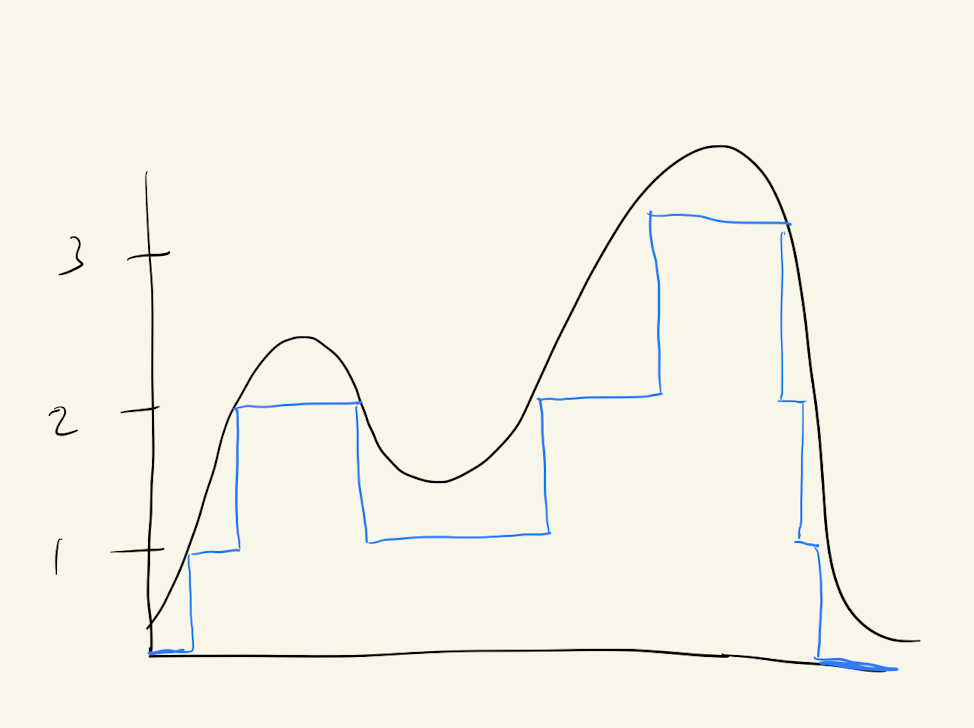
\includegraphics[width=.4\textwidth]{images/simple_function_approximating_non_negative_function}	
\caption{A simple function approximating a non-negative function in terms of its integral}
\end{figure}

\begin{remark}{\remarktitle{When does the integral of a non-negative Borel measurable function exist?}}
The integral of a non-negative Borel measurable function \textit{always} exists (although it may take on the value $+\infty$).  Note that neither case discussed in Remark \ref{rk:when_does_integral_of_simple_function_exist} apply, since the supremum is simply taken over the set of simple functions that never take on negative values. 
\label{rk:when_does_integral_of_non_negative_Borel_measurable_function_exist}
\end{remark}


\paragraphnewline{Properties of integral of non-negative Borel measurable functions (Part I)}

We will use these basic properties below:
\begin{proposition}
Let $f,g$ be non-negative Borel measurable functions. Then
\begin{alphabate}
\item (monotonicity) $\ds\int f \leq \ds\int g \text{ whenever } f \leq g$
\item (non-negative constant multiples) $\ds\int cf = c \ds\int f \text{ for all } c \geq 0.$	
\end{alphabate}
\label{prop:properties_of_integrals_of_non_negative_borel_measurable_functions}
\end{proposition}

\begin{proof}
\begin{alphabate}
\item 
\ifActive
\textbf{Workshop exercise: Prove monotonicity.}
\else 
	\begin{align*}
	f \leq g & \implies \set{s : s \text{ simple } , 0 \leq s \leq f} \subset \set{s:  s \text{ simple } , 0 \leq s \leq g} \\
	& \implies	\set{ \ds\int s \wrt{\mu}  :   s \text{ simple } , 0 \leq s \leq f} \subset \set{ \ds\int s \wrt{\mu} :  s \text{ simple } , 0 \leq s \leq g} && \tinytext{monotonicity for simple fns} \\
	& \implies \sup \set{ \ds\int s \wrt{\mu}  :  s \text{ simple } , 0 \leq s \leq f} \leq  \sup \set{ \ds\int s \wrt{\mu} :   s \text{ simple } , 0 \leq s \leq g} && \tinytext{Prop. \ref{prop:sup_and_inf_for_subsets_are_tighter}} \\
	& \implies \ds\int f \wrt{\mu} \leq \ds\int g \wrt{\mu} && \tinytext{def. integral for non-negative fns}
	\end{align*}
\fi 
\item 
\begin{align*}
\ds\int c f \wrt{\mu} &= \sup \set{\ds\int s' \wrt{\mu} : s' \text{ simple } , 0 \leq s' \leq cf} \\
&=  \sup  \set{\ds\int cs \wrt{\mu}   : s\text{ simple } , 0 \leq s \leq f} && \tinytext{Let $s' = cs$} \\
&= \sup  \set{c \ds\int s \wrt{\mu}   : s\text{ simple } , 0 \leq s \leq f} && \tinytext{Linearity of integral of simple functions} \\
&= c \set{ \ds\int s \wrt{\mu}   : s\text{ simple } , 0 \leq s \leq f} && \tinytext{Prop. \ref{prop:supremum_and_infimum_under_constant_multiples_of_sets}}\\
&= c \ds\int f \wrt{\mu} 
\end{align*}
% By Proposition \ref{prop:borel_measurability_closed_under_multiplication_and_addition} and Example \ref{ex:constant_functions_are_measurable},  $cf$ is a measurable function. Now 
\end{alphabate}

\end{proof}

\paragraphnewline{Computing the integral of non-negative Borel measurable functions}

The following proposition may provide additional confidence in Definition \ref{def:integral_of_non_negative_Borel_measurable_function}, since simple functions approximate non-negative Borel measurable functions.

\begin{proposition}\textbf{(Any non-negative Borel measurable function is the pointwise limit of a sequence of simple functions.)}
Let $h$ be a non-negative Borel measurable function.  Then there is a sequence $\set{s_n}$ of simple functions such that $0 \leq s_1 \leq s_2 \leq ... \leq h$, $s_n \to h$ pointwise, and $s_n \to h$ uniformly on any set on which $h$ is bounded.	
\label{prop:there_is_a_sequence_of_simple_fucntions_that_increases_to_any_non_negative_borel_measurable_function}
\end{proposition}

\begin{proof}
Define 
\[ s_n(\omega) = 
\begin{cases}
\df{k-1}{2^n}, & \text{ if } \quad \df{k-1}{2^n} \leq h(\omega) \leq \df{k}{2^n},\quad k=1,2,...,n2^n \\
n, & \text{ if } \quad h(\omega) \geq n 
\end{cases}
\]	

\begin{figure}[H]
\centering
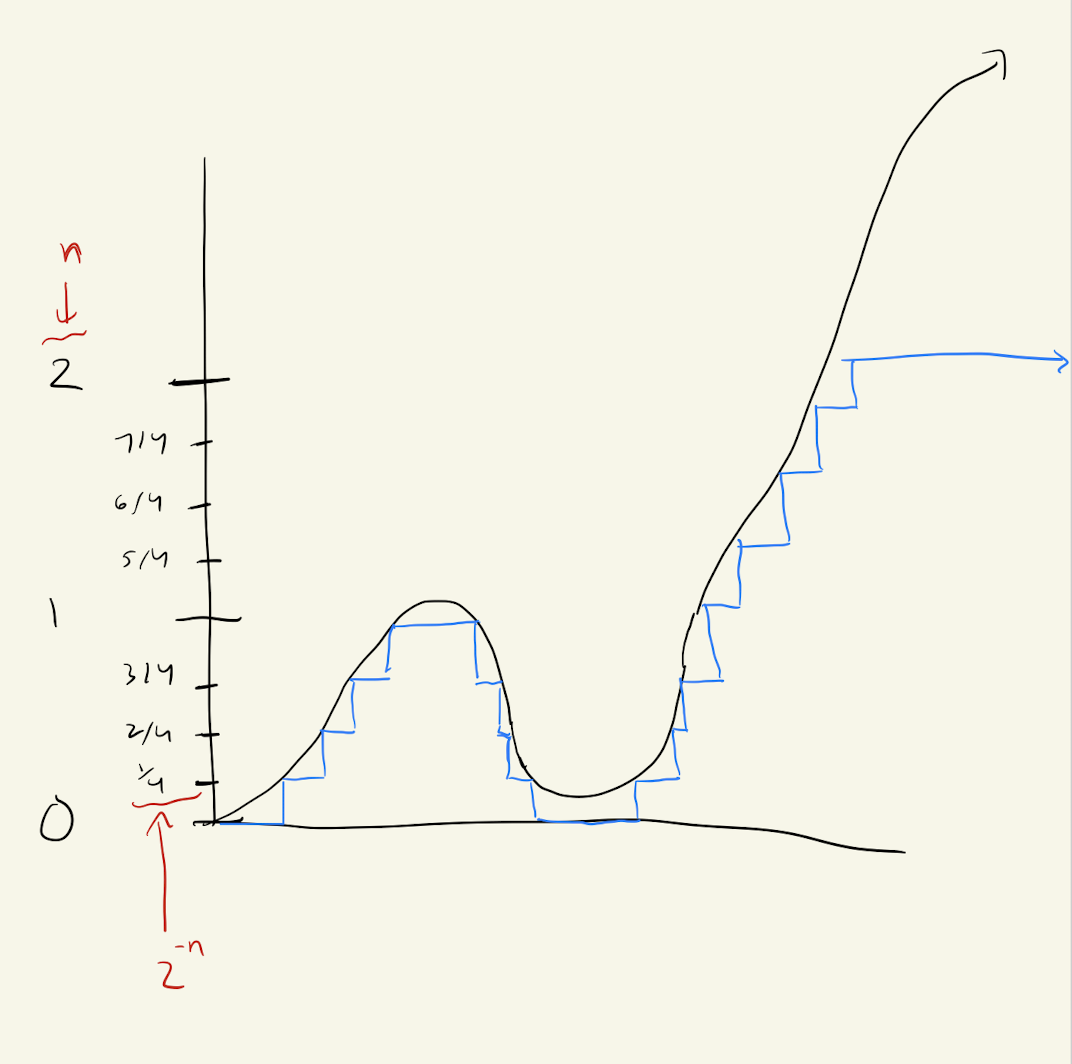
\includegraphics[width=.7\textwidth]{images/approximate_nonnegative_with_simple}	
\caption{An element of an increasing sequence of simple functions approximating an arbitrary non-negative Borel measurable function. The $n$th function in the sequence has a maximum value of $n$ and divides the range into bins of size $2^{-n}$.}
\end{figure}


Then 
\begin{itemize}
\item $s_n \leq s_{n+1}$ for all $n$
\item $0 \leq h - s_n \leq 2^{-n}$ on the set where $h \leq n$.
\end{itemize}
\end{proof}

\begin{question}
When working with $\overline{\R}$, how does one check convergence of a function at a point $\omega$ such that $h(\omega)=\infty$?  Does the proof of Proposition \ref{prop:there_is_a_sequence_of_simple_fucntions_that_increases_to_any_non_negative_borel_measurable_function} still work at such points?
\end{question}

\begin{corollary}{\remarktitle{A Borel measurable function is the limit of a sequence of simple functions which it dominates.}}
An arbitrary Borel measurable function $f$ is the limit of a sequence of finite-valued simple functions $s_n$, with $|s_n|<|f|$ for all $n$.
\label{cor:measurable_function_is_limit_of_simple_functions_which_it_dominates}
\end{corollary}

\begin{proof}
Straightforward. See \cite[Theorem 1.5.5b]{ash2000probability}.	
\end{proof}


Now we establish one of the fundamental convergence theorems. 

\begin{theorem}{\textbf{The Monotone convergence theorem.}}
If $\set{h_n}$ is a sequence of non-negative Borel measurable functions such that $h_n \leq h_{n+1}$ for all $n$ and $h =\lim_{n \to \infty} h_n (= \sup_n h_n)$, then 
\begin{align*}
\ds \int h_n \wrt{\mu} \uparrow \ds\int h \wrt{\mu}
\labelit \label{eqn:monotone_convergence_theorem_conclusion}	
\end{align*}
\label{thm:monotone_convergence_theorem}
\end{theorem}

\begin{proof}

We break the proof into four parts.  Consider
\begin{align*}
\ds \int h \wrt{\mu} = \lim_{n \to \infty} \ds\int h_n \wrt{\mu}
\labelit \label{eqn:monotone_convergence_theorem_pre_conclusion}	
\end{align*}

\begin{itemize}
\item We first show that both quantities in \eqref{eqn:monotone_convergence_theorem_pre_conclusion} exist. First, recall from Remark \ref{rk:when_does_integral_of_non_negative_Borel_measurable_function_exist} that the integral of a non-negative Borel measurable function always exists. So the LHS exists because $h$ is Borel measurable (by Proposition \ref{prop:borel_measurability_closed_under_inf_sup_liminf_limsup}) and non-negative.  The RHS exists since each $\int h_n$ exists and is increasing (by monotonicity; see Prop. \ref{prop:properties_of_integrals_of_non_negative_borel_measurable_functions}), and therefore has a limit (possibly $\infty$). 

\item Next, we show $\geq$ for \eqref{eqn:monotone_convergence_theorem_pre_conclusion}; that is we show $\lim_{n \to \infty} \int h_n \leq \int h$.
\[ h_n \leq h \stackreltext{monotonicity}{\implies} \ds\int h_n \leq \ds\int h \stackreltext{limits preserve (non-strict) inequalities}{\implies} \ds\lim_{n \to \infty} \ds\int h_n \leq \ds\int h \]

\item Now, we show $\leq$ for \eqref{eqn:monotone_convergence_theorem_pre_conclusion}; that is we show $\lim_{n \to \infty} \int h_n \geq \int h$.   Let $\alpha \in (0,1)$ and $s$ be a simple function such that $0 \leq s \leq h$.  Now define 
\[ A_n := \set{\omega : h_n(\omega) \geq \alpha s(\omega) }\]
And note that $A_n \uparrow \Omega$.

So
\begin{align*}
 \ds\int h_n  \stackreltext{monotonicity}{\geq} \ds\int_{A_n} h_n \stackreltext{def. $A_n$, monotonicity}{\geq} \ds\int_{A_n} \alpha s \stackreltext{linearity}{=} \alpha   \ds\int_{A_n} s 
 \labelit \label{eqn:intermediate_eqn_from_proof_mct} 
 \end{align*}
   Now we recognize the right hand side as a measure on $A_n$, and since $A_n \uparrow \Omega$, we can apply continuity from below (see Remark \ref{rk:continuity_of_measure_applied_to_measures_given_by_integrals_of_simple_functions_over_sets}), so taking the limit as $n \to \infty$, Equation \eqref{eqn:intermediate_eqn_from_proof_mct} becomes
\[  \ds\lim_{n \to \infty} \ds\int h_n  \geq \alpha \ds\int s \]
Now since the equality holds for all $\alpha <1$, it holds for $\alpha =1$, and so we have
\[   \ds\lim_{n \to \infty}  \ds\int h_n  \geq \ds\int s \]
Since the LHS is an upper bound on the set in the RHS, it must be greater than the least upper bound, so 
\[   \ds\lim_{n \to \infty}  \ds\int h_n  \geq \ds\int h \]
\item Now we know that \eqref{eqn:monotone_convergence_theorem_pre_conclusion} holds.  It just remains to show that \eqref{eqn:monotone_convergence_theorem_pre_conclusion} $\implies$ \eqref{eqn:monotone_convergence_theorem_conclusion}.  By monotonicity, $\int h_{n+1} \wrt{\mu}  \geq \int h_{n} \wrt{\mu}$ for all $n$, and since the limit of an increasing sequence is its supremum (Prop. \ref{prop:limit_of_monotone_sequences_as_inf_and_sup}), $\int h \wrt{\mu}  \geq \int h_{n} \wrt{\mu}$ for all $n$.
\end{itemize}
\end{proof}


\begin{remark}{\remarktitle{The monotone convergence theorem aids in computation.}}
The monotone convergence theorem can actually be used to make it easier to do computations with integrals of non-negative Borel measurable functions!  Let us quote \cite{folland1999real} (except with changes of notation and references)

\begin{quotation}
 The definition of $\int h$  involves the supremum over a huge (usually uncountable) family of simple functions, so it may be difficult to evaluate $\int h$ directly from the definition (see Definition \ref{def:integral_of_non_negative_Borel_measurable_function}).  The monotone convergence theorem, however, assures us that to compute $\int h$, it is enough to compute $\lim \int s_n$, where $\set{s_n}$ is any sequence of simple functions that increase to $h$, and Proposition \ref{prop:there_is_a_sequence_of_simple_fucntions_that_increases_to_any_non_negative_borel_measurable_function} guarantees that such sequences exist. 
\end{quotation}
\end{remark}

\begin{remark}{\remarktitle{Monotone convergence theorem fails for the Riemann integral.}}
Using an enumeration of the rational numbers between 0 and 1, we define the function $f_n$ (for all nonnegative integer $n$) as the indicator function of the set of the first $n$ terms of this sequence of rational numbers. The increasing sequence of functions $f_n$ (which are nonnegative, Riemann-integrable with a vanishing integral\redfootnote{TODO: Justify that each $f_n$ is Riemann integrable.}) pointwise converges to the Dirichlet function which is not Riemann-integrable (see Remark \ref{rk:dirichlet_function_is_not_Riemann_integrable}).
\end{remark}

\paragraphnewline{Properties of integral of non-negative Borel measurable functions (Part II)}

With the monotone convergence theorem in hand, we can now provide some additional properties of the integrals of non-negative Borel measurable functions.

\begin{proposition}{\textbf{Additivity of integration with non-negative Borel measurable functions.}}
Let $f, g$ be non-negative Borel measurable functions. Then
\[ \ds\int f + \ds\int g = \ds\int f+g \]
\label{prop:additivity_of_integral_for_non_negative_Borel_measurable_functions}
\end{proposition}

\begin{proof}
By Proposition \ref{prop:there_is_a_sequence_of_simple_fucntions_that_increases_to_any_non_negative_borel_measurable_function}, there are sequences of simple functions $\set{s_n}, \set{t_n}$ such that $s_n \uparrow f$ and $t_n \uparrow g$.   Thus, by limit properties, $(s_n + t_n) \uparrow (f+g)$.  So we have
\begin{align*}
	\ds\int f + \ds\int g &=\ds\lim_{n \to \infty} \ds\int s_n + \ds\lim_{n \to \infty} \ds\int t_n && \tinytext{Monotone convergence theorem} \\
	&= \ds\lim_{n \to \infty} ( \ds\int s_n +  \ds\int t_n ) && \tinytext{Sum of limits is limit of sum} \\
	&=  \ds\lim_{n \to \infty} \ds\int (s_n + t_n)  && \tinytext{Linearity of integral for simple functions}\\
	&= \ds\int (f+g)  && \tinytext{Monotone convergence theorem}
 \end{align*}
\end{proof}

Below we show that Proposition \ref{prop:additivity_of_integral_for_non_negative_Borel_measurable_functions} actually extends to linearity with countably infinite sums. 

\begin{corollary}{\remarktitle{Linearity with countably infinite sums of non-negative measurable functions}}
If $\set{f_n}$ is a sequence of non-negative measurable functions,  and 
\[ f(\omega) = \ds\sum_{n=1}^\infty f_n(\omega), \quad \quad \text{ for all } \omega \in \Omega  \]
Then 
\begin{align*}
 \dint_\Omega f \dmu = \ds\sum_{n=1}^\infty \ds\int_\Omega f_n \dmu 
\labelit \label{eqn:consequence_of_linearity_with_countably_infinite_sums_of_non_negative_measurable_functions}	
\end{align*}
Thus, any series of non-negative Borel measurable functions may be integrated term by term.

% Below is Ash's formulation of the statement.  I've replaced it with Rudin's, as I trust Rudin more :)
% 
%If $h_1, h_2, ...$ are non-negative Borel measurable, 
%\[ \ds\int_\Omega \bigg(  \ds\sum_{n=1}^\infty h_n \bigg) \dmu  = \ds\sum_{n=1}^\infty \ds\int_\Omega h_n \dmu\]
\label{cor:linearity_with_countable_infinite_sums_of_non_negative_functions}
\end{corollary}

\begin{proof}
By induction, the linearity of Proposition \ref{prop:additivity_of_integral_for_non_negative_Borel_measurable_functions} extends to a finite collection $\set{f_n}_{n=1}^N$. Now $\ds\sum_{n=1}^N f_n \uparrow \ds\sum_{n=1}^\infty f_n$, so we apply Monotone Convergence Theorem (MCT)
\[ \explaintermbrace{ $\stackexplain{(additivity)}{=} \dsum_{n=1}^\infty \dint f_n \dmu$}{\dlim_{N \to \infty} \dint \dsum_{n=1}^N f_n \dmu} \stackexplain{(MCT)}{=} \dint \dsum_{n=1}^\infty f_n \dmu \]
\end{proof}

\begin{remark}
If we let $\mu$ be the counting measure on a countable set, the statement of  Corollary \ref{cor:linearity_with_countable_infinite_sums_of_non_negative_functions} becomes a statement about double series of non-negative real numbers (which can be proved by more elementary means) \cite{rudin1987real}:

That is, if $a_{ij} \geq 0$ for $i$ and $j = 1, 2, 3, ...$, then 
\[ \ds\sum_{i=1}^\infty \ds\sum_{j=1}^\infty  a_{ij} = \ds\sum_{j=1}^\infty \ds\sum_{i=1}^\infty  a_{ij} \]

{\tiny More explicitly, on $\Omega =\set{1,2,3,...}$, we define sequence $\set{f_i}$ such that $f_i(j) = a_{ij}$.  Then we define $f = \sum_{i=1}^\infty f_i$, so $f(j) = \sum_{i=1}^\infty f_i(j) = \sum_{i=1}^\infty a_{ij}$.

Then, since $\mu$ is the counting measure, the LHS of  \eqref{eqn:consequence_of_linearity_with_countably_infinite_sums_of_non_negative_measurable_functions} becomes 
\[  \dint_\Omega f(j) \dmu(j) = \dsum_{j=1}^\infty f(j) = \ds\sum_{j=1}^\infty \ds\sum_{i=1}^\infty a_{ij}\]	
and the RHS of \eqref{eqn:consequence_of_linearity_with_countably_infinite_sums_of_non_negative_measurable_functions} is 
\[ \ds\sum_{i=1}^\infty \ds\int_\Omega f_i \dmu = \ds\sum_{i=1}^\infty \ds\sum_{j=1}^\infty a_{ij}. \]
}

\end{remark}


\begin{remark}{\remarktitle{Linearity of integration with non-negative Borel measurable functions.}} The scalar multiple property is given by Prop.~\ref{prop:properties_of_integrals_of_non_negative_borel_measurable_functions}, and the additivity is given by Prop.~\ref{prop:additivity_of_integral_for_non_negative_Borel_measurable_functions}.
\label{rk:integrals_are_linear_over_non_negative_Borel_measurable_function}
\end{remark}


%{rk:continuity_of_measure_applied_to_measures_given_by_integrals_of_simple_functions_over_sets}

\subsubsection{Integrals of arbitrary Borel measurable functions}

Let $h$ be an arbitrary Borel measurable function.   We will express an arbitrary Borel measurable function as as the difference of two non-negative Borel measurable functions.

Define:
\begin{align*}
h^+ &:= \max (h,0) \\
h^- &:= \max (-h,0) \\	
\end{align*}
Then 
\begin{align*}
h &= h^+ - h^- \\
|h| &= h^+ + h^- \\	
\end{align*}

\begin{figure}[H]
\centering
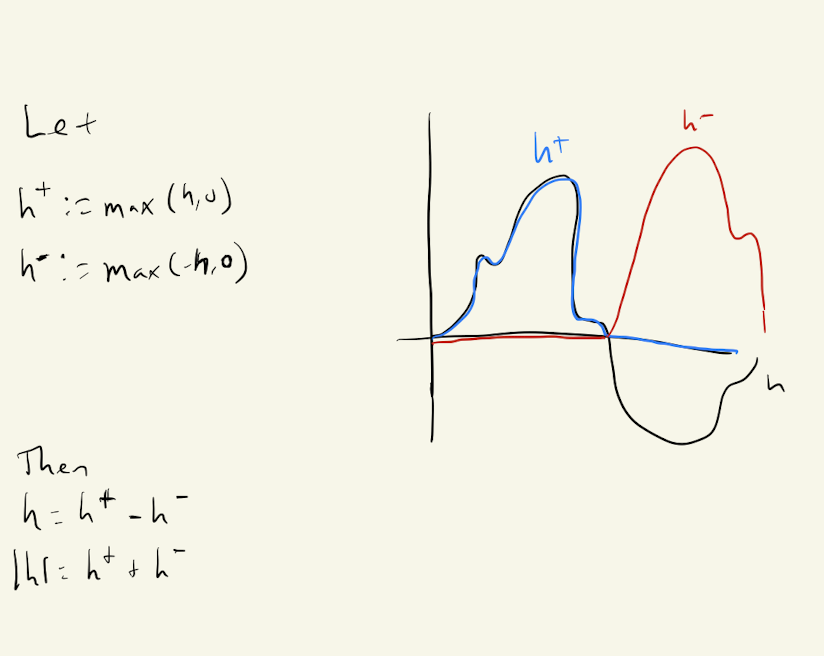
\includegraphics[width=.7\textwidth]{images/arbitrary_borel_measurable_functions_in_terms_of_nonnegative_borel_measurable_functions}
\end{figure}

Now both $h^+$ and $h^-$ are Borel measurable as well.  This holds because if $h_1, h_2$ are Borel measurable, then so are $\max(h_1,h_2)$ and $\min(h_1,h_2)$:

\begin{align*}
\bigg\{ \omega : \max \bigg( h_1(\omega), h_2(\omega) \bigg) < c  \bigg\} &=	\set{\omega :  h_1(\omega) < c } \cap \set{\omega : h_2(\omega) < c } \\
\bigg\{ \omega : \min \bigg( h_1(\omega), h_2(\omega) \bigg)  < c \bigg\} &=	\set{\omega :  h_1(\omega) < c } \cup \set{\omega : h_2(\omega) < c }
\end{align*}


which is sufficient to show measurability by the ``computational definition of measurability" (see Remark \ref{rk:computational_definition_of_Borel_measurability}). 

So we have expressed an arbitrary Borel measurable function as as the difference of two non-negative Borel measurable functions. Therefore, we can define its integral as follows.  

\begin{definition}{\remarktitle{Integral of an arbitrary Borel measurable function}}
\begin{align} 
 \ds\int_\Omega h \wrt{\mu} = \ds\int_\Omega h^+ \wrt{\mu} - \ds\int_\Omega h^- \wrt{\mu} 
\label{eqn:definition_of_integral_of_arbitrary_borel_measurable_function}
\end{align}
\label{def:integral_of_arbitrary_borel_measurable_function}
\end{definition}




\begin{remark}{\remarktitle{When does the integral of an arbitary Borel measurable function exist?}}
Recall from Remark \ref{rk:when_does_integral_of_non_negative_Borel_measurable_function_exist} that the integral of a non-negative Borel measurable function \textit{always} exists (although it may take on the value $+\infty$).  Thus, the integral of an arbitrary non-negative Borel function exists so long as it does not take the form $+\infty - \infty$. 
\label{rk:when_does_integral_of_arbitary_Borel_measurable_function_exist}
\end{remark}

\begin{definition}{\remarktitle{Integrable and extended integrable functions.}}
We say that a function $h$ is $\mu$-integrable (or just integrable if $\mu$ is understood) if $
\ds\int_\Omega h \wrt{\mu}$ is finite, that is, iff $
\ds\int_\Omega h^+ \wrt{\mu}$ and $
\ds\int_\Omega h^- \wrt{\mu}$ are both finite.   %We can express this condition as 
%\[ \bigg| \dint h \dmu \bigg| \stackrel{def. integral}{=} \bigg| \dint h^+ \dmu - \dint h^- \dmu \bigg| < \infty \]
Following \cite[pp.~86]{folland1999real}, we say that a function $h$ is extended $\mu$-integrable iff at least one of $
\ds\int_\Omega h^+ \wrt{\mu}$ and $
\ds\int_\Omega h^- \wrt{\mu}$ are finite (which means that the integral $\ds\int_\Omega h \wrt{\mu}$ exists).
\label{def:integrable_and_extended_integrable_functions}
\end{definition}

\begin{remark}{\remarktitle{Integrals on subsets}}
For $A \in \F$, we define 
\[ \ds\int_A h \wrt{\mu} = \ds\int_\Omega  h \indicate{A} \wrt{\mu} \]
This definition works because whenever $h$ is measurable, then so is $h \indicate{A}$:
\[\set{ \omega : h \indicate{A} (\omega) < c } =	\explaintermbrace{$\in \F$ since $h$ measurable}{\set{\omega :  h(\omega) < c }} \cap \explaintermbrace{$\in \F$ by assumption}{\set{\omega : \omega \in A }} \\  \]
\end{remark}

\begin{example}{\remarktitle{Sums as integrals against counting measure.}}
\cite[pp.89 and Problem 1a (real part only) pp.94]{ash2000probability}.  
Let $\Omega = \set{1,2,3, ...}$, $\F=2^\Omega$ (i.e. all subsets of $\Omega$), and $\mu$ be the counting measure. 
\ifActive
\textbf{Workshop Exercise}: Show that in this setting, the integral is sum.
\else 
	A real-valued function $f$ on $\Omega$ can be written as a sequence of real numbers; we write $f=\set{a_n}, n=1,2, \hdots$.  We will show that an integral on this space is really a sum:
	%
	\begin{align}
	\int_\Omega f \dmu = \ds\sum_{n=1}^\infty a_n	
	\label{eqn:sums_as_integrals}
	\end{align}
	%
	where the series is interpreted as $\sum_{n=1}^\infty a_n^+ - \sum_{n=1}^\infty a_n^-$ if this is not of the form $\infty - \infty$ (if it is, the integral does not exist).\footnote{Recall that $a_n^+ := \max(a_n,0)$ and $a_n^- := \max(-a_n,0)$.}
	
	To justify \eqref{eqn:sums_as_integrals}, let us first assume that $a_n \geq 0$ for each $n$.  We define a sequence of non-negative functions $\set{f_k}$ by $f_k : n \mapsto f(n) \indicate{n \leq k}$, i.e. $f_k = (a_1, a_2, \hdots, a_k, 0, 0, \hdots)$.   
	
	We know how to integrate each $f_k$, since by the definition of integrals of simple functions, we have
	%
	\begin{align}
	 \int f_k \dmu = \ds\sum_{i=1}^k a_i 
	\label{eqn:intermediate_quantity_in_proof_of_integrals_as_sums}
	\end{align}
	%
	Since $f_k \uparrow f$, we apply Monotone Convergence Theorem to obtain
	\begin{align}
	\ds\int f \dmu \stackexplain{def $f$}{=} \ds\int \lim_{k \to \infty} f_k \dmu \stackexplain{MCT}{=}    \ds\lim_{k \to \infty} \ds\int  f_k \dmu \stackexplain{\eqref{eqn:intermediate_quantity_in_proof_of_integrals_as_sums}}{=} \ds\lim_{k \to \infty}  \ds\sum_{i=1}^k a_i = \ds\sum_{i=1}^\infty a_i 
	\label{eqn:second_intermediate_quantity_in_proof_of_integrals_as_sums}
	\end{align}
	%
	Relaxing the non-negativity assumption to allow $a_n \in \R$, we then have
	%
	\begin{align*}
	\int f \dmu &= \int f^+ \dmu - \int f^- \dmu && \tinytext{Def. integral of arbitrary measurable functions}\\
	&= \ds\sum_{i=1}^\infty a_i^+  - \ds\sum_{i=1}^\infty a_i^- && \tinytext{Result with non-negative functions, \eqref{eqn:second_intermediate_quantity_in_proof_of_integrals_as_sums}}
	\end{align*}
	%
	which exists whenever this does not take the form $\infty - \infty$. 
\fi 
\label{ex:integrals_as_sums}
\end{example}



\begin{remark}{\remarktitle{Conditionally convergent sums are not integrals.}}
When summation is considered from the point of Lebesgue integration theory, series that converge conditionally but not absolutely are ignored.\footnote{The alternating harmonic series $\sum_{n=1}^\infty \frac{(-1)^{n-1}}{n}$ is an example of a series that converges conditionally but not absolutely. It is (potentially) easier for series with both negative and positive terms to converge, because terms with different signs may partially cancel or compensate.  See \url{https://www.sfu.ca/math-coursenotes/Math\%20158\%20Course\%20Notes/sec\_AbsoluteConvergence.html}.} 

To see this, note that the expression $\int f \dmu = \sum_{n=1}^\infty a_n^+ - \sum_{n=1}^\infty a_n^-$ from \eqref{eqn:sums_as_integrals} yields four cases

\begin{enumerate}
\item 	$\sum_{n=1}^\infty a_n^+ = \infty,  \sum_{n=1}^\infty a_n^- < \infty$.  The series diverges to $\infty$ and the integrals is $\infty$.
\item  $\sum_{n=1}^\infty a_n^+ < \infty,  \sum_{n=1}^\infty a_n^- = \infty$. The series diverges to $-\infty$ and the integrals is $-\infty$.
\item $\sum_{n=1}^\infty a_n^+ < \infty,  \sum_{n=1}^\infty a_n^- < \infty$. The series is absolutely convergent and the integral equals the sum of the series.
\item  $\sum_{n=1}^\infty a_n^+ = \infty,  \sum_{n=1}^\infty a_n^- = \infty$. The series is not absolutely convergent; it may or may not converge conditionally.  Whether it does or not, the integral does not exist.
\end{enumerate}
\end{remark}


\subsubsection{Properties of the integral of arbitrary Borel measurable functions} \label{sec:properties_of_integral_of_arbitrary_Borel_measurable_functions}

\begin{proposition}
Let $f,g,h$ arbitrary Borel measurable functions. Then
\begin{alphabate}
\item \label{item:scalar_multiple}  (Scalar multiple.) If $\int f \wrt{\mu}$ exists and $c \in \R$, then $\int cf$ exists and $\int cf \wrt{\mu} = c \int f \wrt{\mu} $. %$\ds\int cf \wrt{\mu} = c \ds\int f \wrt{\mu} \text{ for all } c \in \R.$ \quad {\tiny (More explicitly, if $\int f \wrt{\mu}$ exists and $c \in \R$, then $\int cf$ exists and $\int cf \wrt{\mu} = c \int f \wrt{\mu} $.)}
\item \label{item:monotonicity} (Monotonicity.)  If $g \geq h$ and both integrals exist, then $\ds\int g \wrt{\mu} \geq  \ds\int h \wrt{\mu}$. Moreover, if  $g \geq h$,  $\ds\int h \wrt{\mu}$ exists and $\ds\int h \wrt{\mu} > -\infty$, then $\ds\int g \wrt{\mu}$ exists.  And if  $g \geq h$, $\ds\int g \wrt{\mu}$ exists and $\ds\int g \wrt{\mu} < \infty$, then $\ds\int h \wrt{\mu}$ exists.\footnote{We might consider this as a ``dominance criterion for existence."  For more on why the monotonicity statement is concerned with existence, see Remark \ref{rk:why_does_existence_matter_for_monotonicity}.} 
\item \label{item:triangle_inequality_for_integrals}(Triangle inequality for integrals.) If $\int_\Omega h \dmu$ exists, then $|\int_\Omega h \dmu| \leq \int_\Omega |h| \dmu$.
\item \label{item:delayed_truncation_of_simple_functions} (Delayed truncation of simple functions.) If $h \geq 0$ and $B \in \F$, then\footnote{For why this needs to be proven, see Remark \ref{rk:why_delayed_truncation_of_simple_functions_is_something_that_needs_to_be_proven}.} 
\[ \ds\int_B h \wrt{\mu} = \sup \biggset{ \ds\int_B s \wrt{\mu} : \; 0 \leq s \leq h, \; s \text{ simple }} \]
\item \label{item:existence_transfers_to_subsets}(Existence of integral transfers to subsets.) 
\begin{align}
\ds\int_{\Omega} h \wrt{\mu} \text{ exists } &\implies 	\ds\int_{A} h \wrt{\mu} \text{ exists} \quad \forall A \in \F \\
\ds\int_{\Omega} h \wrt{\mu} \text{ finite } &\implies 	\ds\int_{A} h \wrt{\mu} \text{ finite} \quad \forall A \in \F
\end{align}

\end{alphabate}
\label{prop:properties_of_integrals_of_arbitrary_borel_measurable_functions}
\end{proposition}

\begin{proof}
\begin{alphabate}
\item Since $cf$ is a Borel measurable function\footnote{The function $cf$ is a Borel measurable fucntion by Proposition \ref{prop:borel_measurability_closed_under_multiplication_and_addition} and Example \ref{ex:constant_functions_are_measurable}.  Alternatively, we could verify this directly.  If $c \geq 0$, then $\set{\omega : c f(\omega) \leq k} = \set{\omega : f(\omega) \leq k/c} \in \F$ by the Borel measurability of $f$.  Similarly if  $c < 0$, then $\set{\omega : c f(\omega) \leq k} = \set{\omega : f(\omega) \geq k/c} \in \F$ by the Borel measurability of $f$.}, we apply Definition \ref{def:integral_of_arbitrary_borel_measurable_function}.

We have 
\begin{subequations}
\begin{align}
\text{if $c \geq 0$}, && (cf)^+ &= cf^+  & (cf)^- &= cf^-   \label{eqn:decomposing_scalar_multiple_of_borel_measurable_function_into_two_nonnegative_functions_when_scalar_multiple_is_nonnegative} \\
\text{if $c < 0$}, && (cf)^+ &= -cf^-  & (cf)^- &= -cf^+. \label{eqn:decomposing_scalar_multiple_of_borel_measurable_function_into_two_nonnegative_functions_when_scalar_multiple_is_negative} 
\end{align}
\end{subequations}

\begin{figure}[H]
\centering
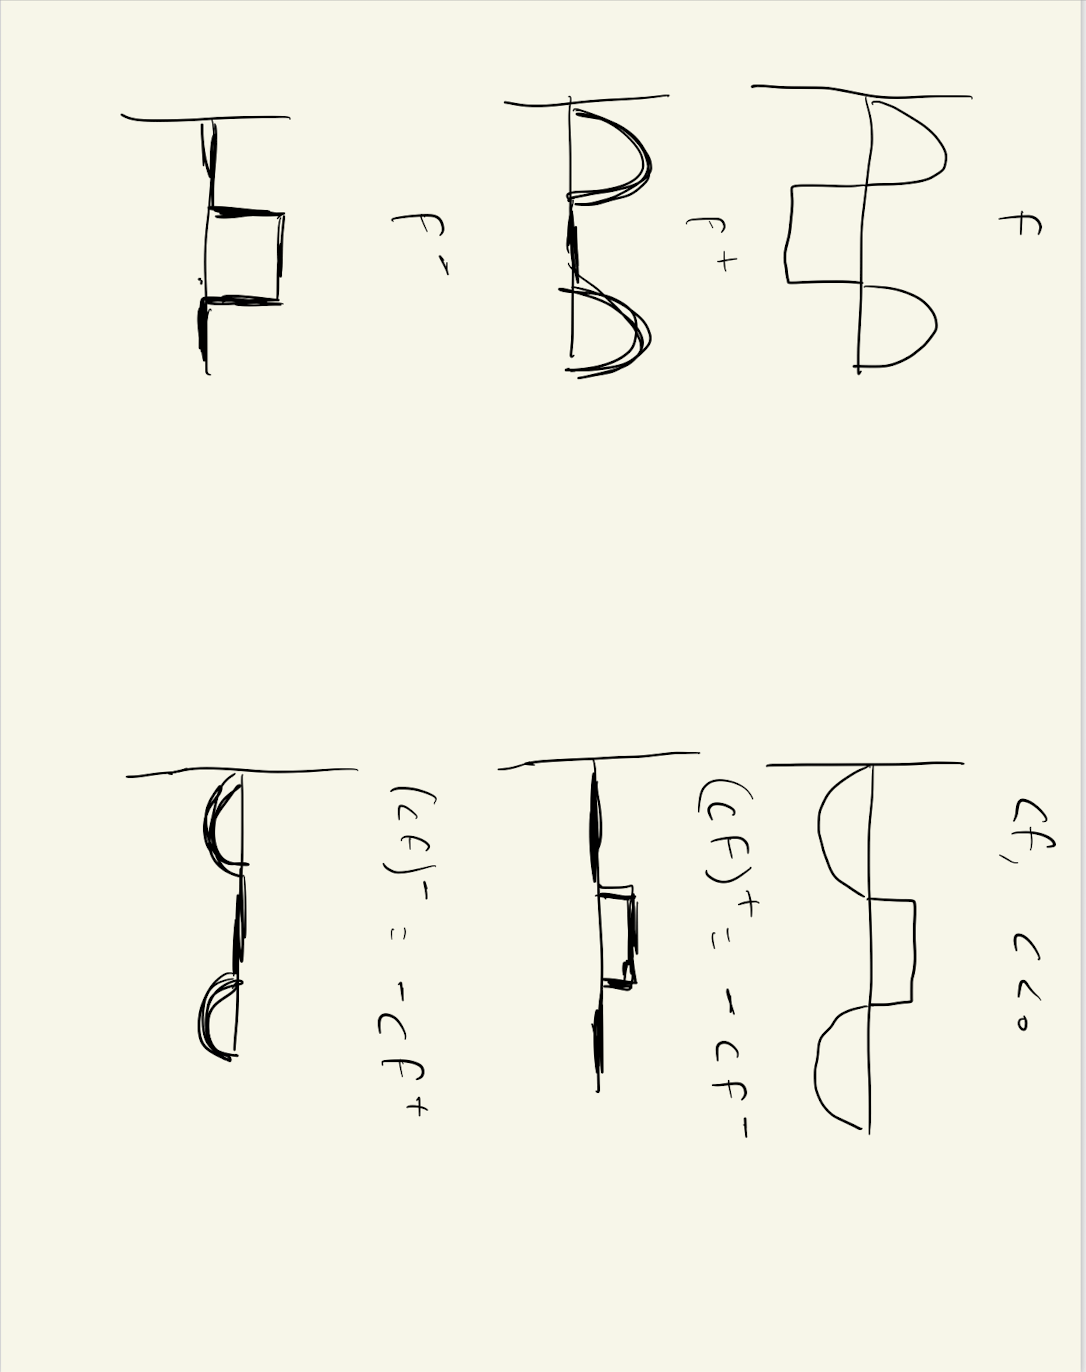
\includegraphics[width=.5\textwidth, angle=90]{images/decomposing_scalar_multiple_of_borel_measurable_function_into_two_nonnegative_functions_when_scalar_multiple_is_negative}	
\end{figure}


Now we will use the fact that if $f$ is non-negative Borel measurable and $c \geq 0$, then we already know the identity holds (see Prop. \ref{prop:properties_of_integrals_of_non_negative_borel_measurable_functions} (b)).


So if $c\geq 0$
\begin{align*}
\ds\int cf \wrt{\mu} &= \ds\int (cf)^+ \wrt{\mu} - \ds\int (cf)^- \wrt{\mu} && \tinytext{Def. \ref{def:integral_of_arbitrary_borel_measurable_function}} \\
&= \ds\int cf^+ \wrt{\mu} - \ds\int cf^- \wrt{\mu} && \tinytext{\eqref{eqn:decomposing_scalar_multiple_of_borel_measurable_function_into_two_nonnegative_functions_when_scalar_multiple_is_nonnegative}} \\ 
& \stackrel{*}{=} c \ds\int f^+ \wrt{\mu} - c \ds\int f^- \wrt{\mu} && \tinytext{ Prop. \ref{prop:properties_of_integrals_of_non_negative_borel_measurable_functions} (b)} \\ %\labelit \label{eqn:expanding_integral_of_nonnegative_scalar_times_function} \\
& = c \ds\int f \wrt{\mu} && \tinytext{Def. \ref{def:integral_of_arbitrary_borel_measurable_function}} 
\end{align*}

Likewise if $c < 0$
\begin{align*}
\ds\int cf \wrt{\mu} &= \ds\int (cf)^+ \wrt{\mu} - \ds\int (cf)^- \wrt{\mu} && \tinytext{Def. \ref{def:integral_of_arbitrary_borel_measurable_function}} \\
&= \ds\int -cf^- \wrt{\mu} - \ds\int -cf^+ \wrt{\mu} && \tinytext{\eqref{eqn:decomposing_scalar_multiple_of_borel_measurable_function_into_two_nonnegative_functions_when_scalar_multiple_is_negative}} \\ 
& \stackrel{**}{=} -c \ds\int f^- \wrt{\mu} + c \ds\int f^+ \wrt{\mu} && \tinytext{ Prop. \ref{prop:properties_of_integrals_of_non_negative_borel_measurable_functions} (b)}  \\ %\labelit \label{eqn:expanding_integral_of_positive_scalar_times_function} \\
& = c \ds\int f \wrt{\mu} && \tinytext{Def. \ref{def:integral_of_arbitrary_borel_measurable_function}} \\
\end{align*}	

Equations (*) and (**) reveal that $\int cf \wrt{\mu}$ exists whenever $\int f \wrt{\mu}$ exists.

\item First we show that $g \geq h \implies \ds\int g \wrt{\mu} \geq \ds\int h \wrt{\mu}$ when both integrals exist.  We decompose each function into its positive and negative parts
\[ g = g^+ - g^-, \quad h = h^+ - h^-. \]
By hypothesis,
\[ g^+ \geq h^+, \quad g^- \leq h^-. \]
So by monotonicity for non-negative functions (Prop. \ref{prop:properties_of_integrals_of_non_negative_borel_measurable_functions} (a)), we have 
\begin{align} \ds\int g^+ \wrt{\mu} \geq \ds\int h^+ \wrt{\mu}, \quad \ds\int g^- \wrt{\mu}  \leq \ds\int h^- \wrt{\mu}. 
\label{eqn:monotonicity_for_positive_and_negative_parts_separately}
\end{align}

So
\begin{align*}
\ds\int g \wrt{\mu} &= 	\ds\int g^+ \wrt{\mu} - \ds\int g^- \wrt{\mu} && \tinytext{(def. integral; existence assumed)} \\
&\geq \ds\int h^+ \wrt{\mu} - \ds\int h^- \wrt{\mu} &&  \tinytext{\eqref{eqn:monotonicity_for_positive_and_negative_parts_separately}} \\
&=\ds\int g \wrt{\mu} && \tinytext{(def. integral;  existence assumed)}
\end{align*}

Now we consider the ``dominance criterion for existence".  We prove the second sentence of (b), as the third is proved similarly. 

If $\ds\int h \wrt{\mu}$ exists and $\ds\int h \wrt{\mu} > -\infty$, then by definition of the integral, $\ds\int h^- \wrt{\mu} < \infty$.  Since $g \geq h$, then $g^- \leq h^-$, so 
\[ \ds\int g^- \wrt{\mu} \leq \ds\int h^- \wrt{\mu} < \infty \]
Thus, $\ds\int g \wrt{\mu}$ exists.\footnote{Recall that for $\ds\int f \wrt{\mu}$ to exist, at least one of  $\ds\int f^- \wrt{\mu}$, $\ds\int f^+ \wrt{\mu}$ must be finite.}
\item We have $-|h| \leq h \leq |h|$.  So by monotonicity and the scalar multiple property, $- \int_\Omega |h| \dmu \leq \int_\Omega h \dmu \leq \int_\Omega |h| \dmu$.  By multiplying the left-hand inequality by -1 and keeping the right-hand inequality as is, we see  
\[ - \int_\Omega h \dmu \leq \int_\Omega |h| \dmu  \quad \text { and } \quad \int_\Omega h \dmu \leq \int_\Omega |h| \dmu  \] 
which taken together says $|\int_\Omega h \dmu| \leq \int_\Omega |h| \dmu$.
\item  We want to prove that if $h \geq 0$ and $B \in \F$, then
\[ \ds\int_B h \wrt{\mu} = \sup \biggset{ \ds\int_B s \wrt{\mu} : \; 0 \leq s \leq h, \; s \text{ simple }}. \] 
We prove \framebox{$\geq$}, \framebox{$\leq$}  separately, using the strategy of Remark \ref{rk:one_way_to_show_two_supremums_are_equal}.

\begin{itemize}
\item \framebox{$\geq$}.  For $0 \leq s \leq h$, $s$ simple,
\begin{align*}  
\ds\int_B h \wrt{\mu} \geq \ds\int_B s \wrt{\mu}  && \tinytext{monotonicity}
\end{align*}
Since the LHS is an upper bound on the set of the integrals on the RHS, \framebox{$\geq$} holds. 

\item \framebox{$\leq$} 
\begin{align*}
\set{t: t \text{ simple}, 0 \leq t \leq h \indicate{B}}  & \subseteq \set{s \indicate{B} : s \text{ simple }, 0 \leq s \leq h }  \\
\implies \explaintermbrace{:=$\ds\int_B h \wrt{\mu}$}{\sup \biggset{\ds\int t  \wrt{\mu} : \; t \text{ simple}, \; 0 \leq t \leq h \indicate{B} }} & \leq \sup \biggset{\ds\int s \indicate{B} \wrt{\mu} : \; s \text{ simple}, \; 0 \leq s \leq h } 
\end{align*}

\end{itemize}

\item 
\[ (h \indicate{A})^+ = h^+\indicate{A} \, \leq h^+, \quad  (h \indicate{A})^- = h^- \indicate{A}  \, \leq h^- \]
So by monotonicity,
\begin{align*}
\explaintermbrace{A1}{\ds\int (h \indicate{A})^+ \wrt{\mu}} \leq \explaintermbrace{B1}{\ds\int h^+ \wrt{\mu}} \\
\explaintermbrace{A2}{\ds\int (h \indicate{A})^- \wrt{\mu}} \leq \explaintermbrace{B1}{\ds\int h^- \wrt{\mu}} \\
\end{align*}
So $B_i < \infty \implies A_i < \infty$.

By assuming the conditional holds for at least one $i \in \set{1,2}$, we prove transfer of existence. By assuming the conditional holds for both $i$, we prove transfer of finiteness. 

\end{alphabate}
\end{proof}




\begin{remark}{\remarktitle{Why the monotonicity property is concerned with existence.}}
Why is Proposition \ref{prop:properties_of_integrals_of_arbitrary_borel_measurable_functions} \ref{item:monotonicity} concerned with monotonicity? Answer: even if $\ds\int g \wrt{\mu}$ exists and $g \geq h$, we can still have $\ds\int h \wrt{\mu}$ not exist, because of \eqref{eqn:monotonicity_for_positive_and_negative_parts_separately}.  For example, we can have 
\begin{align}
\ds\int g^+ \wrt{\mu} &= \ds\int h^+ \wrt{\mu} = \infty  \\
\ds\int g^- \wrt{\mu} & < \ds\int h^- \wrt{\mu} = \infty 	
\end{align}
and so $\ds\int h \wrt{\mu}$ DNE.
\label{rk:why_does_existence_matter_for_monotonicity}
\end{remark}

\begin{remark}{\remarktitle{Why delayed truncation of simple functions is something that needs to be proven.}}
Proposition \ref{prop:properties_of_integrals_of_arbitrary_borel_measurable_functions} \ref{item:delayed_truncation_of_simple_functions} needs to be proven because it is \textit{not} what is given by the definition of the integral for an arbitrary Borel measurable function (after observing that $h \indicate{B}$ is still measurable).   Note that
\begin{subequations}
\begin{align}	
\ds\int_\Omega h \wrt{\mu} &= \sup \biggset{ \ds\int s \wrt{\mu} : \; 0 \leq s \leq h \indicate{B}, \; s \text{ simple} } && \tinytext{def. integral} \label{eqn:integral_over_subset_according_to_definition} \\
\ds\int_\Omega h \wrt{\mu} &= \sup \biggset{ \ds\int s \indicate{B} \wrt{\mu} : \; 0 \leq s \leq h, \; s \text{ simple}  }&& \tinytext{Prop. \ref{prop:properties_of_integrals_of_arbitrary_borel_measurable_functions}  \ref{item:delayed_truncation_of_simple_functions}. } \label{eqn:integral_over_subset_according_to_delayed_truncation_property}
\end{align}
\end{subequations}

\begin{figure}[H]
\centering 
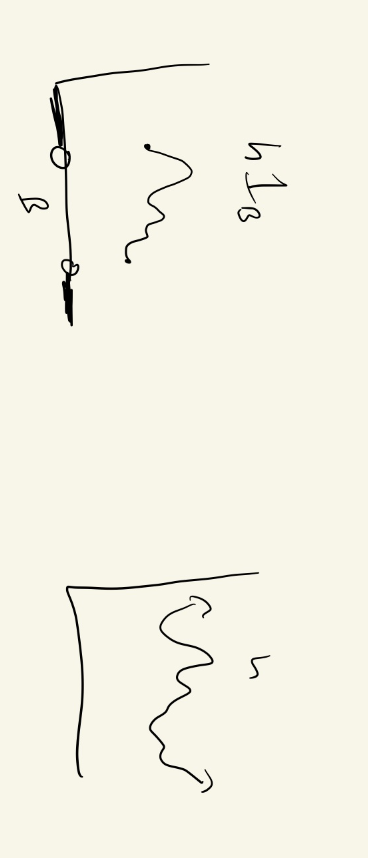
\includegraphics[width=.2\linewidth, angle=90]{images/function_and_truncated_function}	
\end{figure}

What does each say?
\begin{itemize}
\item \eqref{eqn:integral_over_subset_according_to_definition} : truncate first, then ``simplify"
\item \eqref{eqn:integral_over_subset_according_to_delayed_truncation_property} ``simplify" first, then truncate
\end{itemize}


\label{rk:why_delayed_truncation_of_simple_functions_is_something_that_needs_to_be_proven}.
\end{remark}
 
\begin{example}{\remarktitle{A simple example of triangle inequality for integrals.}}
Let $h(x) = \sin(x)$, $A=[0,2\pi]$, and $\mu$ be Lebesgue measure. Then 
\begin{figure}[H]
\centering 
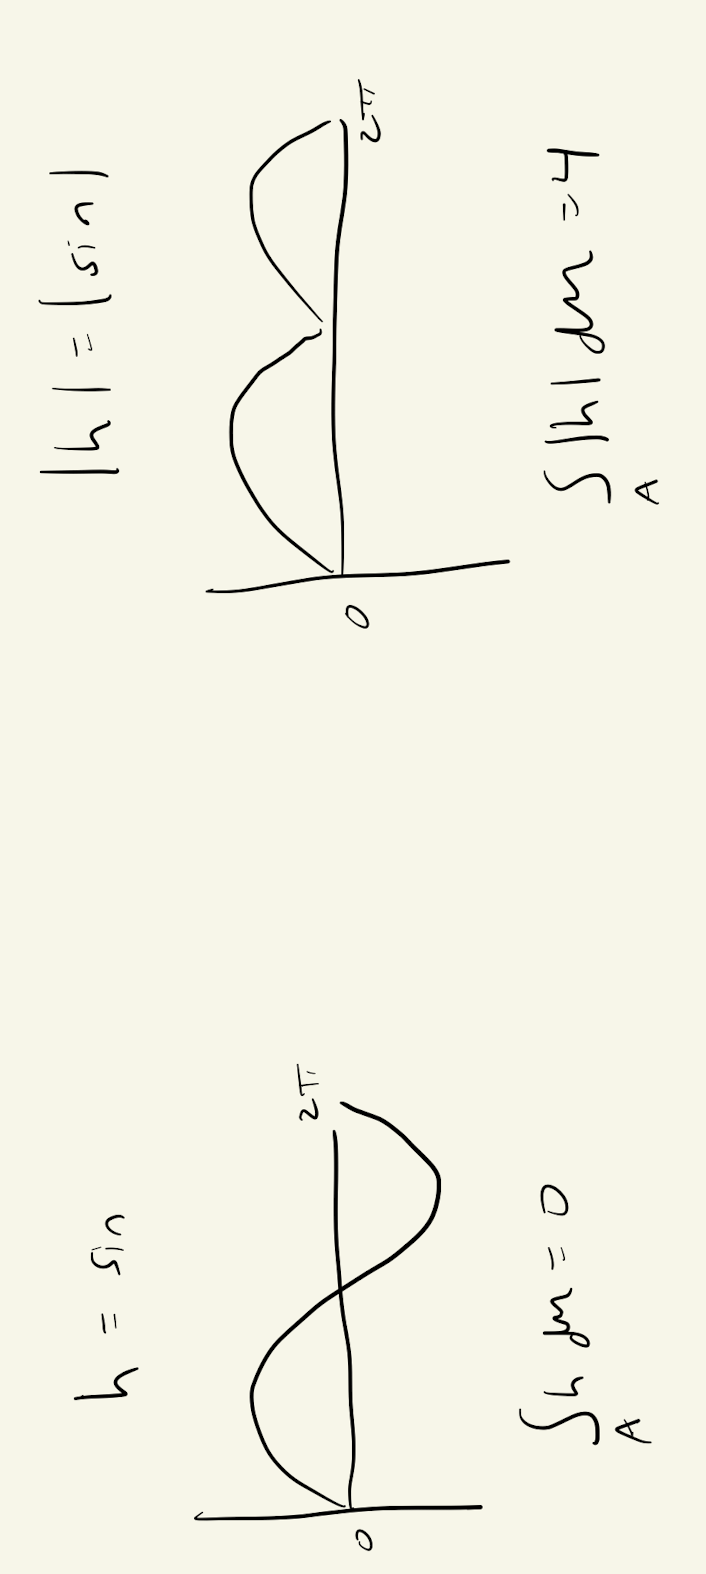
\includegraphics[width=.2\linewidth, angle=270]{images/triangle_inequality_for_integrals}	
\end{figure}
The basic idea is that integrating over a function $h$ that can take on both positive and negative values can lead to cancelations, which explains the result.	
\label{ex:simple_example_of_triangle_inequality}
\end{example}

 
\section{$\S$ 1.6 Basic Integration Theorems}

Here we prove some basic integration theorems, and further properties of integration that can be derived thereof.  %Note that we have already provided the Monotone Convergence Theorem and Fatou's lemma in the previous section (since we give statements that apply to non-negative functions). 

\subsection{Indefinite integrals as countably additive set functions}

\begin{definition}
We say that $\lambda$ is an \textit{indefinite integral}\footnote{This interpretation of ``indefinite integral" is used in \cite[pp.~61]{ash2000probability}}  with respect to $\mu$ if for any $A \in \F$ we have
%
\begin{align*}
\lambda(A)  =  \ds\int_A f \dmu
\labelit \label{eqn:indefinite_integral}
\end{align*}
where $f$ is a Borel measurable function and where $\int_\Omega f \dmu$ exists.
\label{def:indefinite_integrals}	
\end{definition}

\begin{theorem}{\textbf{Indefinite integrals are countably additive set functions.}}
Let $f$ be a Borel measurable function such that $\int_\Omega f \wrt{\mu}$ exists.  Define $\lambda(B) = \int_B f \wrt{\mu}$, $B \in \F$.  Then $\lambda$ is countably additive on $\F$; thus if $f \geq 0$, $\lambda$ is a measure.	
\label{thm:integrals_are_countably_additive_set_functions}
\end{theorem}

\begin{proof}
Recall that Prop. \ref{prop:the_integral_of_a_simple_function_over_a_set_is_one_way_to_measure_that_set}  proved this for non-negative simple functions.


So let $f$ be any non-negative Borel measurable function.   We want to show that if $\lambda(B) = \int_B f \wrt{\mu}$,  $B = \bigcupdot_{n=1}^\infty B_n$, then $\lambda(B) = \ds\sum_{n=1}^\infty \lambda(B_n)$.

\begin{itemize}
\item \framebox{$\leq$} Let $s$ be simple, $0 \leq s \leq f$.   Then 
\begin{align*}
\ds\int_B s \wrt{\mu} &= \ds\sum_{n=1}^\infty \ds\int_{B_n} s \wrt{\mu} && \tinytext{Prop. \ref{prop:the_integral_of_a_simple_function_over_a_set_is_one_way_to_measure_that_set}} \\
&\leq \ds\sum_{n=1}^\infty \ds\int_{B_n} f \wrt{\mu}  && \tinytext{monotonicity} \\ 
&:= \ds\sum_{n=1}^\infty \lambda(B_n) 	
\end{align*}
Since the RHS is an upper bound, the supremum (over s) cannot exceed it.  Thus, applying Prop. \ref{prop:properties_of_integrals_of_arbitrary_borel_measurable_functions} \ref{item:delayed_truncation_of_simple_functions}, we have 
\begin{align*}
\ds\int_B f \wrt{\mu} & \leq \ds\sum_{n=1}^\infty \lambda(B_n)  \\ 
\implies \lambda(B) &\leq \ds\sum_{n=1}^\infty \lambda(B_n) && \tinytext{def. $\lambda$}
\end{align*}

\item \framebox{$\geq$}	By monotonicity of the integral, 
\begin{align*}
B \supset B_n \implies \indicate{B} \geq \indicate{B_n} \implies  f\indicate{B}   \geq f\indicate{B_n} \implies \lambda(B) \geq \lambda(B_n) && \tinycircled{1}
\end{align*} 
If $\lambda(B_n) =\infty$ for one $n$, we are done. {\tiny (Why? Since $f \geq 0$, by monotonicity, $\int_A f \wrt{\mu} \geq 0$ for any $A \in \F$.  So each $\lambda(B_n) \geq 0$.  So if one $\lambda(B_n) = \infty$, then $\sum_{n=1}^\infty \lambda(B_n) = \infty$, and \tinycircled{1} and $\lambda(B) \geq \ds\sum_{n=1}^\infty \lambda(B_n)$ are saying the same thing, that $\lambda(B) = \infty$.)}
 
 So let each $\lambda(B_n) < \infty$.  
 
 Fix $N$.  Consider $\bigcupdot_{n=1}^N B_n$.  By Prop. \ref{prop:properties_of_integrals_of_arbitrary_borel_measurable_functions} \ref{item:delayed_truncation_of_simple_functions} and properties of the supremum {\tiny (if we subtract $\epsilon$ from it, there $\exists$ a member of the set exceeding that)}, for all $\epsilon>0$, we have simple functions $s_n : 0 \leq s_n \leq f$ for each $n$ so that 
 
\begin{align*}
\ds\int_{B_n} s_n \wrt{\mu} \geq \ds\int_{B_n} f \wrt{\mu} - \frac{\epsilon}{N} \quad \text{ for all } n  && \tinycircled{2} 
\end{align*}
Let $s^*$ be the pointwise maximum of $\set{s_n}_{n=1}^N$.  This is still a simple function, and $s^* \indicate{B_n} \geq s_n \indicate{B_n}$ for each $n$, so 
   
\begin{align*}
\ds\int_{B_n} s^* \wrt{\mu} \geq \ds\int_{B_n} s_n \quad \text{ for all } n && \tinycircled{3}
\end{align*}

So \tinycircled{2} and \tinycircled{3} gives that 
 
\begin{align*}
\ds\int_{B_n} s^* \wrt{\mu} \geq \ds\int_{B_n} f \wrt{\mu} - \frac{\epsilon}{N} \quad \text{ for all } n  && \tinycircled{4} 
\end{align*}

Thus, for any $N$, $\epsilon>0$, we have  
\begin{align*}
\lambda(B) &\geq \lambda(\bigcupdot_{n=1}^N B_n) && \tinytext{By monotonicity; need argument like \tinycircled{1}; we don't know it's a measure yet!} \\
&:= \ds\int_{\bigcupdot_{n=1}^N B_n} f \wrt{\mu} \\
& \geq \ds\int_{\bigcupdot_{n=1}^N B_n} s^* \wrt{\mu} && \tinytext{monotonicity} \\
&= \ds\sum_{n=1}^N \ds\int_{B_n} s^* \wrt{\mu} && \tinytext{what's we're trying to prove holds for simple functions (Prop. \ref{prop:the_integral_of_a_simple_function_over_a_set_is_one_way_to_measure_that_set}) } \\
&\geq \ds\sum_{n=1}^N \ds\int_{B_n} f_n \wrt{\mu} - \epsilon && \tinytext{see \tinycircled{4}} \\
&:= \ds\sum_{n=1}^N  \lambda(B_n) -\epsilon \\
\implies \lambda(B) &\geq \ds\sum_{n=1}^\infty \lambda(B_n) && \tinytext{justified below}
\end{align*}

{\tiny What justifies the last line above?  \textbf{Claim.} Let $\set{a_n}_{n=1}^\infty : 0 \leq a_n < \infty$.  Then $M \stackrel{*}{\geq} \ds\sum_{n=1}^N a_n - \epsilon \; \text{ for any } N, \epsilon>0 \implies M \geq \ds\sum_{n=1}^\infty a_n.$ \textbf{Proof}. If $\ds\sum_{n=1}^\infty a_n = \infty$ then the claim obviously holds.  If $\ds\sum_{n=1}^\infty a_n < \infty$ then for all $\epsilon >0$, the tail of the series is less than $\epsilon$ for some $N^*$.  So write $\sum_{n=1}^{N^*} a_n < \ds\sum_{n=1}^\infty a_n - \epsilon$, and equation (*) becomes $M \geq \ds\sum_{n=1}^\infty a_n - 2\epsilon = \ds\sum_{n=1}^\infty a_n -\tilde{\epsilon}$ for all $\tilde{\epsilon} > 0$.  Take the limit as $\tilde{\epsilon} \to 0$, and the non-strict inequality is preserved in the limit.}

So now assume $f$ is an arbitrary Borel-measurable function.  Since we have assumed $\ds\int f \wrt{\mu}$ exists, we have $\ds\int f^+ \wrt{\mu}, \ds\int f^- \wrt{\mu} < \infty$.  So by what we have shown for non-negative functions, there exists measures $\lambda^+, \lambda^-$ corresponding to each of these integrals.  So if $B = \bigcupdot_{n=1}^\infty B_n$, 
\begin{align*}
\ds\int_B f \wrt{\mu} &= \ds\int_B f^+ \wrt{\mu} - \ds\int_B f^- \wrt{\mu} && \tinytext{def. integral} \\
\implies \lambda(B) &= \lambda^+(B) - \lambda^-(B) && \tinytext{by def. of $\lambda$, $\lambda^+$, $\lambda^-$ } \\
\implies \lambda(B) &= \ds\sum_{n=1}^\infty \lambda^+(B_n) - \ds\sum_{n=1}^\infty \lambda^-(B_n) && \tinytext{by result with non-negative functions } \\
\end{align*}
 and this expression is \textit{NOT} of the form $\infty - \infty$, since the first line isn't, by the existence of $\int_\Omega f \wrt{\mu}$ {\tiny (and the fact that, by monotonicity, $\int_\Omega f \wrt{\mu} < \infty \implies \int_B f \wrt{\mu} < \infty  $) }.

\end{itemize}

\end{proof}

\begin{corollary}{\textbf{Indefinite integrals as measures.}}
Let $f \geq 0$ be a Borel measurable function such that $\int_\Omega f \wrt{\mu}$ exists.  Define $\lambda(B) = \int_B f \wrt{\mu}$, $B \in \F$.  Then $\lambda$ is a measure.	
\label{cor:indefinite_integrals_as_measures}
\end{corollary}

\begin{proof}
We apply Definition \ref{def:measure} to show that $\lambda$ is a measure.   $\lambda$ is countably additive by Theorem \ref{thm:integrals_are_countably_additive_set_functions}.  
The non-negativity of $\lambda$ is immediate from Definition \ref{def:integral_of_non_negative_Borel_measurable_function}. 
\end{proof}



\begin{remark}{\textbf{Indefinite integrals are signed measures.}}
As will become clear in Section~\ref{sec:signed_measures}, Theorem \ref{thm:integrals_are_countably_additive_set_functions} more generally tells us that \textit{indefinite integrals are signed measures}.	 If we remove the constraint that $f \geq 0$, then $\lambda$ is a countably additive set function, but it may be negative. 

The Radon-Nikodym theorem (to be covered later in the document) provides an important converse:  instead of obtaining a signed measure $\lambda$ from a measure $\mu$ and function $f$, we will be given signed measure $\lambda$ and measure $\mu$, and will obtain the \textit{Radon-Nikodym derivative} $f$.
\end{remark}


% NOTE: I was previously trying to make this remark about change of signed measure as well, but (1) I ran into some existence questions that don't exist when integrating non-negative functions, (2) I felt awkward about it since signed measures don't appear until a later section, (3) At one point I wanted to use the extended MCT, which hasn't been introduced yet, (4) I wasn't 100% sure that I was stating things correctly and minimally, since I was trying to state more than what was stated by Rudin.  So with all this in mind, for now at least, I will just reduce this to a statement about change in measure 
%\begin{remark}{\textbf{Change of measure, change of signed measure, and differential notation.}}
%
%By Theorem~\ref{thm:integrals_are_countably_additive_set_functions}, the indefinite integral 
%%
%\begin{align*}
%\lambda(A)  =  \ds\int_A f \dmu
%\labelit \label{eqn:indefinite_integral_again}
%\end{align*}
% can be interpreted as a change in signed measure; specifically, as a change from measure $\mu$ to signed measure $\lambda$. In the special case where $f \geq 0$, then $\lambda$ is a measure, and so the formula provides a mechanism for change of measure. 
%
%To express this relationship, we sometimes use the following notation \cite[pp.~89]{folland1999real}:
%%
%\begin{align} 
%d\lambda = f \; d\mu 
%\label{eqn:indefinite_integral_in_differential_form}	
%\end{align}
%%
%And sometimes, by a slight abuse of language, we refer to ``the signed measure $f \, d\mu$".
%
%The notation may make more sense if we interpret it as does \cite[pp.~24]{rudin1987real} :
%\begin{align*}
%\dint_A g \wrt{\lambda} = \dint_A g f \dmu
%\labelit \label{eqn:change_of_differential}
%\end{align*}
%for every measurable function $g$ and every measurable set $A$.
%
%
%As pointed out by \cite[pp.~24]{rudin1987real}, we assign no independent meaning to the symbols 
%$d\lambda$ and $d\mu$; \eqref{eqn:indefinite_integral_in_differential_form} simply means that \eqref{eqn:indefinite_integral_again} (and therefore \eqref{eqn:change_of_differential}) holds for every measurable $f$. 
%
%The Radon-Nikodym theorem (to be covered later in the document) provides an important converse:  instead of obtaining a signed measure $\lambda$ from a measure $\mu$ and function $f$, we will be given signed measure $\lambda$ and measure $\mu$, and will obtain the \textit{Radon-Nikodym derivative} $f$.
%
%{\tiny Let us prove \eqref{eqn:change_of_differential} from Theorem \ref{thm:integrals_are_countably_additive_set_functions} in the special case where $f,g \geq 0$.
%
%\begin{itemize}
%	\item First let $g$ be a simple function, which we write as $s= \sum_{i=1}^r x_i \indicate{E_i}$.   Then 
%\[ \int s \wrt{\lambda} \stackexplain{simple f'n}{=} \sum_{i=1}^r x_i \lambda(E_i) \stackexplain{hypothesis}{=}  \sum_{i=1}^r x_i \int_{E_i} f \dmu \stackexplain{linearity}{=} \int \sum_{i=1}^r x_i \indicate{E_i} f \dmu \stackexplain{def. $s$}{=} \int sf \dmu    \]
%\item Now let $g$ be a non-negative measurable function. By Prop \ref{prop:there_is_a_sequence_of_simple_fucntions_that_increases_to_any_non_negative_borel_measurable_function}, there exists a sequence of simple functions $\set{s_n}$ such that $s_n \uparrow g$.  Since  $s_n \uparrow g$, then also $s_n f \uparrow fg$.  So applying Monotone Convergence Theorem to both, we obtain $\int s_n d\lambda \uparrow \int g d\lambda$ and  $\int s_n f d\mu \uparrow \int fg d\mu$.  But since $\int s_n d\lambda  =\int s_n f d\mu$ for all $n$ by the previous bullet point, the sequences must have the same limit (by uniqueness of limits), so $\int g d\lambda = \int gf d\mu$.
%\end{itemize}
%} 
%\label{rk:change_of_measure_and_differential_notation}
%\end{remark}


\begin{remark}{\textbf{Change of measure and differential notation.}}

 By Cor.~\ref{cor:indefinite_integrals_as_measures},  given Borel measurable $f \geq 0$, the indefinite integral 
%
\begin{align*}
\lambda(A)  =  \ds\int_A f \dmu
\labelit \label{eqn:indefinite_integral_again}
\end{align*}
 can be interpreted as a change in measure specifically, as a change from measure $\mu$ to measure $\lambda$. 
 
To express this relationship, we sometimes use the following notation \cite[pp.~89]{folland1999real}:
%
\begin{align} 
d\lambda = f \; d\mu 
\label{eqn:indefinite_integral_in_differential_form}	
\end{align}
%
And sometimes, by a slight abuse of language, we refer to ``the measure $f \, d\mu$".

The notation may make more sense if we interpret it, as does \cite[pp.~24]{rudin1987real}:
\begin{align*}
\dint_\Omega g \wrt{\lambda} = \dint_\Omega g f \dmu
\labelit \label{eqn:change_of_differential}
\end{align*}
for every measurable function $g$ on $\Omega$.\footnote{Note that if also $g \geq 0$, this constructs yet another measure by $\xi(A) = \int_A g \wrt{\lambda}$ for all $A \in \F$.} (See  Proposition~\ref{prop:change_of_differential} for a proof.) 


As pointed out by \cite[pp.~24]{rudin1987real}, we assign no independent meaning to the symbols 
$d\lambda$ and $d\mu$; \eqref{eqn:indefinite_integral_in_differential_form} simply means that \eqref{eqn:indefinite_integral_again} (and therefore \eqref{eqn:change_of_differential}) holds for every measurable $f \geq 0$. 

\label{rk:change_of_measure_and_differential_notation}
\end{remark}


\begin{example-for-data-scientists}{\remarktitle{Jeffreys prior for observation noise in linear regression}}
An example for statisticians: Jeffreys prior for observation noise in linear regression  (see e.g. \cite{carvalho2010horseshoe} or \cite{makalic2015simple}) is sometimes written as
\begin{align}
 \sigma^2 &\sim \sigma^{-2} \wrt{\sigma^2} \label{eqn:prior_on_observation_noise_for_linear_regression_model_with_horseshoe_prior_jeffreys_special_case}
\end{align}
%
What does this mean?  First off, the $\sim$ notation means that the random variable $\sigma^2$ has the probability distribution $P$ described by
\[  dP = \sigma^{-2} \wrt{\mu(\sigma^2)} \]
where $\mu$ is Lebesgue measure. This is differential notation of the form \eqref{eqn:indefinite_integral_in_differential_form}.  Unpacking back to 	\eqref{eqn:indefinite_integral_again}, this is saying that
%\[  P(A) = \ds\int_A \sigma^{-2} \dmu  = \ds\int_A \sigma^{-2} \wrt{\sigma^2} \]	
\[  P(A) = \ds\int_A \sigma^{-2} \dmu  = \ds\int_A \sigma^{-2} \wrt{\sigma^2} \]
for all measurable sets $A$.
\end{example-for-data-scientists}

\subsection{Additivity theorem}
 
\begin{theorem}{\textbf{Additivity theorem.}}
Let $f$ and $g$ be Borel measurable, and assume that $f+g$ is well-defined.  If $\dint_\Omega f \dmu$ and $\dint_\Omega g \dmu$ exist and $\dint_\Omega f \dmu$ + $\dint_\Omega g \dmu$ is well-defined (not of the form $+ \infty - \infty$ or $- \infty +\infty$), then 
\[ \dint_\Omega f +g \dmu = \dint_\Omega f \dmu + \dint_\Omega g \dmu \]
In particular, if $f$ and $g$ are integrable, so is $f+g$.
\label{thm:additivity}
\end{theorem}

\begin{proof}
See \cite{ash2000probability}, Theorem 1.6.3.	
\end{proof}



\begin{remark}{\remarktitle{Additivity holds automatically for integrable functions.}}
If $f$ and $g$ are integrable, the conditions of Theorem \ref{thm:additivity} are always met.    

Moreover, in this situation, the proof of Theorem \ref{thm:additivity} is straightforward. Suppose $f$ and $g$ are integrable. Let $h=f+g$.  Then 
\[ h^+ - h^- = f^+ - f^- + g^+ - g^- \]
Rearranging, we have 
\[ h^+ + f^- + g^- = f^+ + g^+ + h^- \]
Applying additivity for non-negative functions (see Prop. \ref{prop:additivity_of_integral_for_non_negative_Borel_measurable_functions}) twice, we get 
\[ \int h^+ + \int f^- + \int g^- =  \int f^+ + \int g^+ + \int h^- \]
Rearranging (possible by integrability), we get 
\begin{align*} 
\int h^+ -  \int h^- &=  \int f^+ - \int f^- + \int g^+ - \int g^- \\
\stackexplain{def. integral, def. h}{\implies} \int f+g &= \int f + \int g 
\end{align*}
\label{rk:additivity_holds_automatically_for_integrable_functions}	
\end{remark}

\begin{non-example}
Let us demonstrate where the Additivity Theorem fails to apply.  Let $f \equiv 1, g \equiv -1$ and $\mu$ be Lebesgue measure.  Then $\int f \dmu = \infty$ and $\int  g \dmu = -\infty$.  But
\[\begin{array}{rcccl}
\int (f+g) &\dmu  \neq &  \int f \dmu & + & \int g \dmu   \\
	0 && \infty && -\infty 
\end{array} \]
Because $\infty - \infty$ is undefined. {\tiny (To reinforce the undefinedness of  $\infty - \infty$, note that the LHS could be $0$, $\infty$ or $-\infty$ by setting $f \equiv a, g \equiv -b$, by choosing $a<b, b>a$, or $a=b$.) }
\end{non-example}


\begin{remark}{\remarktitle{From additivity to linearity.}}
The conditions of the additivity theorem imply the conditions of the scalar multiple property (Prop \ref{prop:properties_of_integrals_of_arbitrary_borel_measurable_functions} (a)).  Thus, linearity holds whenever additivity holds.
\label{rk:linearity_holds_if_additivity_holds}	
\end{remark}

\begin{proposition}{\remarktitle{Change of differential.}}\footnote{This is Exercise 4 from \cite[pp.~71]{ash2000probability}.}  Let $(\Omega, \F, \mu)$ be a measure space, and $f \geq 0$ a non-negative Borel measurable function on $\Omega$.  Recalling Cor.~\ref{cor:indefinite_integrals_as_measures}, define a measure $\lambda$ on $\F$ by 
\begin{align*}
\lambda(A)  =  \ds\int_A f \dmu
%\labelit \label{eqn:indefinite_integral_yet_again}
\end{align*}
Then for any Borel measurable function $g$ on $\Omega$, we have 
\begin{align*}
\dint_\Omega g \wrt{\lambda} = \dint_\Omega g f \dmu
%\labelit \label{eqn:change_of_differential_in_proposition}
\end{align*}
in the sense that if one of the integrals exists, so does the other, and the two integrals are equal.
% NOTE: I am calling this change of differential instead of change of measure so that the name accommodates arbitrary g and not just non-negative g. 
\label{prop:change_of_differential} 
\end{proposition}

\begin{proof}
We proceed through the steps in constructing the integral.

\begin{alphabate}
	\item \textit{Simple functions.} First let $g$ be a simple function, which we write as $s= \sum_{i=1}^r x_i \indicate{E_i}$.   Then 
\[ \int s \wrt{\lambda} \stackexplain{$\int$ for simple f'n}{=} \sum_{i=1}^r x_i \lambda(E_i) \stackexplain{hypothesis}{=}  \sum_{i=1}^r x_i \int_{E_i} f \dmu \stackexplain{linearity}{=} \int \sum_{i=1}^r x_i \indicate{E_i} f \dmu \stackexplain{def. $s$}{=} \int sf \dmu    \]
\item \textit{Non-negative Borel measurable functions.} Now let $g$ be a non-negative Borel measurable function. By Prop \ref{prop:there_is_a_sequence_of_simple_fucntions_that_increases_to_any_non_negative_borel_measurable_function}, there exists a sequence of simple functions $\set{s_n}$ such that $s_n \uparrow g$.  Since  $s_n \uparrow g$, then also $s_n f \uparrow fg$.  So applying Monotone Convergence Theorem to both, we obtain $\int s_n d\lambda \uparrow \int g d\lambda$ and  $\int s_n f d\mu \uparrow \int fg d\mu$.  But since $\int s_n d\lambda  =\int s_n f d\mu$ for all $n$ by the previous bullet point, the sequences must have the same limit (by uniqueness of limits), so $\int g d\lambda = \int gf d\mu$.
\item \textit{Arbitrary Borel measurable functions.} Now let $g$ be an arbitrary Borel measurable function.
\begin{align*}
 \int g \wrt{\lambda} &\stackexplain{$\int$ for general f'n}{=} \int g^+ \wrt{\lambda} - \int g^- \wrt{\lambda}  \stackexplain{part (b)}{=}  \int g^+ f \wrt{\mu} - \int g^- f \wrt{\mu} \\
  &\stackexplain{Additivity Thm}{=} \int (g^+ - g^-) f \dmu \stackexplain{def. $g^+, g^-$}{=} \int g f \dmu  	
 \end{align*}
 which holds if $ \int g \wrt{\lambda}$ exists.  In that case, $\int g^+ \wrt{\lambda} - \int g^- \wrt{\lambda}$ is well-defined, and so the Additivity Theorem (Thm.~\ref{thm:additivity}) can be applied. 
\end{alphabate}


\end{proof}


\begin{corollary}{\remarktitle{Additivity corollaries}}
\begin{alphabate}
\item If $h$ is Borel measurable, $h$ is integrable iff $|h|$ is integrable.
\item If $g$ and $h$ are Borel measurable with $|g| \leq h$, $h$ integrable, then $g$ is integrable.	
\end{alphabate}
\label{cor:additivity_corollaries}
\end{corollary}

\begin{proof}
\begin{alphabate}
\item  If $h$ is integrable, then by assumption we have 
\[ \bigg| \dint h \dmu \bigg| \stackexplain{def. \, integral}{=} \bigg| \dint h^+ \dmu - \dint h^- \dmu \bigg| < \infty \]
which is true iff BOTH of $\biggset{\dint h^+ \dmu , \dint h^- \dmu } < \infty$

If $|h|$ is integrable, then by assumption we have 
\[ \bigg| \dint |h| \dmu \bigg| \stackexplain{additivity  (Theorem \ref{thm:additivity})}{=} \bigg| \dint h^+ \dmu + \dint h^- \dmu \bigg| < \infty \]
which is also true iff BOTH of $\biggset{\dint h^+ \dmu , \dint h^- \dmu } < \infty$
\item 
\begin{align*}
\dint h \dmu &< \infty &&\tinytext{by hypothesis} \\
\implies \dint |g| \dmu &< \infty &&\tinytext{by monotonicity}	\\
\implies g &\text{ integrable } && \tinytext{by item b) above}	
\end{align*}
\end{alphabate}
\end{proof}

\subsection{Almost everywhere theorems}

\begin{definition}
A condition is said to hold \textbf{almost everywhere} with respect to the measure $\mu$ (written a.e $[\mu]$ or simply a.e. if $\mu$ is understood) if there exists a set $B \in \F$ of $\mu$-measure 0 such that the condition holds outside $B$.
\label{def:almost_everywhere}
\end{definition}

From the point of view of integration theory, functions that differ only on a set of measure zero may be identified, as is established by the following result.

\begin{theorem}{\textbf{Almost everywhere}.}
Let $f,g,h$ be Borel measurable functions.
\begin{alphabate}
\item If $f=0$ a.e. $[\mu]$, then $\dint_\Omega f \dmu =0$.
\item If $g=h$ 	a.e. $[\mu]$, and $\dint_\Omega g \dmu$ exists, then so does $\dint_\Omega h \dmu$, and $\dint_\Omega g \dmu  = \dint_\Omega h \dmu$. 
\end{alphabate}
\label{thm:almost_everywhere}
\end{theorem}

\begin{proof}
\ifActive 
	\textbf{Workshop exercise: Prove part(a) for when $f$ is simple.  If you have time, try proving it for when $f$ is non-negative.}
\else  
	
	\begin{alphabate}
	\item  
	
		\begin{enumerate}
		\item[i)] \underline{$f$ simple}.	 If $f$ is simple, we can write $f=\sum_{i=1}^n x_i \indicate{A_i}$.  By hypothesis, $\forall$ i, $x_i=0$ or $\mu(A_i)=0$.  Thus, $\int f \dmu = \sum_{i=1}^n x_i \indicate{A_i} =0.$
		\item[ii)] \underline{$f$ non-negative}. Since $f=0$ a.e. $[\mu]$, then $\forall$ $s \in \set{s \text{ simple } : 0 \leq s \leq f}, s=0$ a.e. $[\mu]$.  So by item i), $\int s \dmu =0 \, \forall s$.  So by definition of the integral for non-negative functions
		\[ \int f \dmu = \sup \bigg\{ \int s \dmu : s \text{ simple}, 0 \leq s \leq f \bigg\}  = \sup \set{0} = 0\]
		\item[iii)]\underline{$f$ arbitrary}. $f=0$ a.e. $[\mu] \implies f^+=0, f^-=0$ a.e. $[\mu]$.  So by item ii), $\int f^+ \dmu =0, \int f^- \dmu =0.$. So by definition of the integral $ \int f \dmu = \int f^+ \dmu - \int f^- \dmu =0$.
		\end{enumerate}
	\item We prove i) $\int h \dmu$ exists and then that ii) $\int h \dmu = \int g \dmu$
	
		\begin{enumerate}
		\item[i)] $\int g \dmu$ exists means that $\int g^+ \dmu, \int g^- \dmu$ are not BOTH $\infty$.  WLOG, suppose that $\int g^+ \dmu < \infty 	 \quad \tinycircled{1}$.  
		
		Now $h=g$ a.e. $\implies h^+=g^+, h^-=g^-$ a.e. $\implies h^+ - g^+ = 0 \text{ a.e. } \quad \tinycircled{2}$.   So
	\begin{align*}
	0 \stackexplain{by part (a) and \tinycircled{2}}{=} \ds\int (h^+ - g^+) \dmu \stackexplain{linearity}{=} 	\ds\int h^+ \dmu  - \ds\int g^+ \dmu && \tinycircled{3}
	\end{align*}
	where we can apply linearity (see Remark \ref{rk:linearity_holds_if_additivity_holds}) because
		\begin{itemize}
		\item Integrals of non-negative functions always exist, and multiplication by a scalar doesn't change existence (see Prop. \ref{prop:properties_of_integrals_of_arbitrary_borel_measurable_functions} \ref{item:scalar_multiple}).
		\item The difference can't be of the form $\infty - \infty$ by \tinycircled{1}.
		\end{itemize}
	So again by \tinycircled{1}, we can add to  sides of \tinycircled{3} to get
	\[ \dint h^+ = \dint g^+ < \infty \]
	so $\int h \dmu$ exists.
	\item[ii)] Let $A:=\set{\omega : h(\omega) = g(\omega)}$.  By hypothesis, $\mu(A^c)=0$. Now we decompose each function by partitioning their domains
	\begin{align*}
	h&=h\indicate{A} + h\indicate{A^c}  \stackexplain{def. $A$}{=} g \indicate{A} + h \indicate{A^c} \labelit \label{eqn:decompose_h_by_domain}\\
	g&= g\indicate{A} + g\indicate{A^c}  \labelit \label{eqn:decompose_g_by_domain}\\	
	\end{align*}
	 Now since $g \indicate{A^c}, h \indicate{A^c}$ equal 0 except on a set of measure 0, by part (a),
	\begin{align*}
	\int_{A^c} g \dmu =0, \quad  \int_{A^c} h \dmu =0
	\labelit\label{eqn:integrals_on_set_of_measure_zero}	
	\end{align*}
	And so we can apply additivity to \eqref{eqn:decompose_h_by_domain} and \eqref{eqn:decompose_g_by_domain}, since:
		\begin{itemize}
		\item $\int g \dmu, \int h \dmu$ exist, so since existence transfers to subsets (see Prop. \ref{prop:properties_of_LS_measures}\ref{item:existence_transfers_to_subsets}), $\int_A g \dmu, \int_{A^c} g \dmu, \int_A h \dmu, \int_{A^c} h \dmu $ exist.  
		\item By \eqref{eqn:integrals_on_set_of_measure_zero},
		\begin{align*}
		\int_A g \dmu + \int_{A^c} g \dmu & \neq \infty - \infty \\
		\int_A h \dmu + \int_{A^c} h \dmu  & \neq \infty - \infty \\	
		\end{align*}
		\end{itemize}
		So applying linearity to \eqref{eqn:decompose_h_by_domain} and \eqref{eqn:decompose_g_by_domain}, we get 
		\begin{align*}
		\int h \dmu &= 	\int_A g \dmu + 	\cancelto{0}{\int_{A^c} h \dmu} && \tinytext{cancelation by \eqref{eqn:integrals_on_set_of_measure_zero}.} \\
		\int g \dmu &= 	\int_A g \dmu + 		\cancelto{0}{\int_{A^c} g \dmu} && \tinytext{cancelation by \eqref{eqn:integrals_on_set_of_measure_zero}.} \\
		\end{align*}
		And so $\int h \dmu = \int g \dmu$
		\end{enumerate}
	\end{alphabate}
\fi 
\end{proof}

\begin{remark}
	
Thanks to Theorem \ref{thm:almost_everywhere}, in any integration theorem, we may freely use the phrase ``almost everywhere" in the hypotheses, and the conclusions will still follow.  For example
\begin{itemize}
\item If $g,h$ are Borel measurable and $g \geq h$ a.e., then $\int g \dmu \geq \int h \dmu$.  {\tiny (This is the monotonicity property from Prop. \ref{prop:properties_of_integrals_of_arbitrary_borel_measurable_functions} \ref{item:monotonicity}, but with the condition weakened to a.e.). }
\item If $\set{h_n}$ is a sequence of non-negative Borel measurable functions such that $h_n \to h$ a.e., then $\int_\Omega h_n \dmu \to \int_\Omega h \dmu$. {\tiny (This is the Monotone Convergence Theorem but with the condition weakened to a.e.  In more detail: we can simply define $h^*_n$ such that it equals $h_n$ almost everywhere and $h$ on the set of measure 0.  Then $h^*_n \to h$.  So by MCT,  $\int_\Omega h^*_n \dmu \to \int_\Omega h \dmu$.  But by Theorem \ref{thm:almost_everywhere} b), $\int_\Omega h^*_n \dmu  = \int_\Omega h_n \dmu$ for all $n$, and so the conclusion holds.)  }
\end{itemize}
\end{remark}

\begin{theorem}
Let $h$ be Borel measurable.
\begin{alphabate}
\item If $h$ is integrable, then $h$ is finite a.e. 
\item \label{item:integral_of_nonnegative_function_equals_zero_implies_the_function_equals_zero_almost_everywhere} If $h \geq 0$ and $\int_\Omega h \dmu =0$ then $h=0$ a.e.
\end{alphabate}
\label{thm:properties_of_functions_derived_from_properties_of_integrals}
\end{theorem}

\begin{proof}
\begin{alphabate}
\item By contraposition.  If h is not finite a.e., then $\exists B \in \F : \mu(B) >0$ and $|h \indicate{B}| = \infty$.  Then 
\[ \ds\int_\Omega |h| \dmu \stackexplain{monotonicity}{\geq} \ds\int_B |h| \dmu \stackexplain{simple function} = \infty \, \mu(B) = \infty. \]
So $|h|$ is not integrable. So by Corollary \ref{cor:additivity_corollaries} b), $h$ is not integrable. 
\item Let $B_n := \set{\omega : h(\omega) \geq \frac{1}{n}}$.  Then  $ B_n \uparrow B := \set{\omega : h(\omega) > 0}.\footnote{Recall that $\cup_{n=1}^\infty [\frac{1}{n}, \infty) = (0, \infty)$.} \quad \tinycircled{1}$

Now
\begin{align*} 
 0 \stackexplain{first hypothesis}{\leq} h \indicate{B_n} \stackexplain{$B_n \subset B$ }{\leq} h \indicate{B} \stackexplain{def. $B$}{=} h \\
\implies \dint_{B_n} h \dmu \stackexplain{monotonicity}{\leq} \dint_\Omega h \dmu \stackexplain{second hypothesis}{=} 0 \\
\stackexplain{first hypothesis, monotonicity}{\implies} \dint_{B_n} h \dmu =0 && \tinycircled{2}
\end{align*}
Now \tinycircled{1} and monotonicity again give
\begin{align*}
\dint_{B_n} h \dmu \stackexplain{def. $B_n$, monotonicity}{\geq} \dint \frac{1}{n} \indicate{B_n} \dmu \stackexplain{simple function}{=} \frac{1}{n} \mu(B_n) && \tinycircled{3} 	
\end{align*}
Now \tinycircled{2} and \tinycircled{3} together give $\mu(B_n) =0 \; \forall n$.  So by continuity of measure
\[ \mu(B) = \ds\lim_{n \to \infty} \mu(B_n) =0 \]

\end{alphabate}
	
\end{proof}

We can now construct a converse to monotonicity. 

\begin{theorem}{\textbf{Monotonicity Converse.}}
If $\mu$ is $\sigma$-finite on $\F$, $g$ and $h$ are Borel measurable, $\int_\Omega g \dmu$ and $\int_\Omega h \dmu$ exist, and $\int_A g \dmu \leq \int_A h \dmu$ for all $A \in \F$, then $g \leq h$ a.e. $[\mu]$.
\label{thm:monotonicity_converse}
\end{theorem}

\begin{proof}
We prove the theorem assuming that at least one of $\set{ \int_\Omega g \dmu,  \int_\Omega h \dmu}$ is finite (so that we can apply the Additivity Theorem).  Note that in this special case, we need not assume that 	$\mu$ is $\sigma$-finite on $\F$.  For a full proof, see \cite{ash2000probability} Theorem 1.6.11.

Let $A:=\set{x : g(x) < h(x)}$. {\tiny (Note that $A$ is the set where the desired conclusion fails.)}  Then 
\[\ds\int_A g \dmu \stackexplain{monotonicity on $A$}{\leq} \ds\int_A h \dmu \stackexplain{hypothesis}{\leq} \ds\int_A g \dmu \]
So by sandwiching, 
\[ \ds\int_A g \dmu  = \ds\int_A h \dmu. \] 
Now 
\[ 0 \stackexplain{subtraction}{=} \ds\int_A h \dmu  - \ds\int_A g \dmu \stackexplain{linearity} =  \ds\int_A (h-g) \dmu\] 
where linearity applies under the assumptions of the theorem. {\tiny (It wouldn't apply if $\ds\int_A g \dmu = \infty, \ds\int_A h \dmu = -\infty$, or vice versa, which would violate the conditions of the additivity theorem.)}

So 
\[\begin{array}{rcl}
0 = 	\ds\int \explaintermbrace{non-negative by def $A$}{(h-g) \, \indicate{A}} \dmu &\stackexplain{Theorem~\ref{thm:properties_of_functions_derived_from_properties_of_integrals}~\ref{item:integral_of_nonnegative_function_equals_zero_implies_the_function_equals_zero_almost_everywhere}}{\implies}  &  (h-g)\indicate{A} = 0 \; \text{a.e.} \\
& \implies & (h-g) = 0 \quad \text{ a.e. on } A \\
& \implies & h=g \quad \text{a.e. on } A
\end{array} \]

This gives an a.e. contradiction to the definition of $A$.  So $\mu(A)=0$. 
\end{proof}

\begin{remark}{\remarktitle{On the assumptions of the monotonicity converse.}}
 By monotonicity (Prop.~\ref{prop:properties_of_integrals_of_arbitrary_borel_measurable_functions}), $g \leq h$ implies $\int_\Omega g \dmu \leq \int_\Omega h \dmu$, and in fact, $\int_A g \dmu \leq \int_A h \dmu$ for all $A \in \F$ {\tiny (This holds by monotonicity again, since $g \leq h \implies g \indicate{A} \leq h \indicate{A}$.)}  Now note that $\int_\Omega g \dmu \leq \int_\Omega h \dmu  \red{\notimplies} \int_A g \dmu \leq \int_A h \dmu$ for all $A \in \F$. (To see this, consider that $g,h$ are not necessarily non-negative.  So for a counter-example, just take $g=\sin$ and $h=0$ when integrating with respect to Lebesgue measure.  See also Example \ref{ex:simple_example_of_triangle_inequality}.)  So we obtain the converse by imposing the condition that the integral inequality holds over all measurable sets. 	
\end{remark}

\begin{remark}
In the proof of the monotonicity converse, we derived an ``a.e. contradiction" to a set to show it has measure 0 seems like a fun proof technique.  I haven't seen this before. 
\end{remark}

\begin{remark}
This remark could be made in many places, but note from the proof of the monotonicity converse how convenient it is to work with Lebesgue integrals rather than than Riemann integrals for proving integral properties.  We can define some set $A$ in the domain to have any desired property, and then proceed to work with it. 
\end{remark}


\begin{corollary}
If $\mu$ is $\sigma$-finite on $\F$, $g$ and $h$ are Borel measurable, $\int_\Omega g \dmu$ and $\int_\Omega h \dmu$ exist, and $\int_A g \dmu = \int_A h \dmu$ for all $A \in \F$, then $g = h$ a.e. $[\mu]$.
\label{cor:equal_integrals_for_all_measurable_sets_implies_the_functions_are_equal_ae}
\end{corollary}

\begin{proof}
 Since $\int_A g \dmu = \int_A h \dmu$ for all $A \in \F$, we have  
\begin{align*}
\int_A g \dmu \leq \int_A h \dmu 	& \stackexplain{Thm.~\ref{thm:monotonicity_converse}}{\implies} g \leq h \; \text{a.e.} \\
\text{ and} \int_A h \dmu \leq \int_A g \dmu 	& \stackexplain{Thm.~\ref{thm:monotonicity_converse}}{\implies} h \leq g \; \text{a.e.}
\end{align*}
Hence $g=h$ a.e.
\end{proof}

\begin{remark}
Cor.~\ref{cor:equal_integrals_for_all_measurable_sets_implies_the_functions_are_equal_ae} gives a statent in Prop 2.2.3 b) of \cite{folland1999real}, but that statement assumes that both $g$ and $h$ are both integrable, whereas here we only need to assume that the integrals exist.  	
\end{remark}


\subsection{Extended monotone convergence theorem}


The monotone convergence theorem as stated earlier only applies to non-negative functions and only to increasing sequences. We relax those assumptions below.

\begin{theorem}{\textbf{Extended Monotone Convergence Theorem.}}
Let $f_1, f_2, ..., f, g$ be Borel measurable
\begin{alphabate}
\item If $f_n \uparrow f$ and $f_n \geq g$ for all $n$, where $\int_\Omega g \dmu > -\infty$, then 
\[ \ds\int_\Omega f_n \dmu \uparrow \ds\int_\Omega f \dmu  \]
\item If $f_n \downarrow f$ and $f_n \leq g$ for all $n$, where $\int_\Omega g \dmu < \infty$, then 
\[ \ds\int_\Omega f_n \dmu \downarrow \ds\int_\Omega f \dmu  \]	
\end{alphabate}
\label{thm:extended_monotone_convergence_theorem}
\end{theorem}

\begin{proof}
\begin{alphabate}
\item If $\int g \dmu = \infty$, then by monotonicity {\tiny (and the fact that the limit of an increasing sequence equals its supremum)}, $\int f \dmu \geq \int f_n \dmu \geq \int g \dmu$, and the conclusion holds.  So assume $\int g \dmu < \infty$.  Along with the hypothesis, we have that $\int g \dmu$ is finite.

%Now we have $f_n - g \geq 0$ and $f_n -g \uparrow f-g$, so by Monotone Convergence Theorem, 
Now
\begin{align*}
& f_n - g \geq 0 \quad \text{ and } \quad f_n -g \uparrow f-g && \tinytext{Hypothesis (and Prop \ref{prop:limit_of_monotone_sequences_as_inf_and_sup})} \\
\implies & \ds\int (f_n - g) \dmu \uparrow \ds\int (f-g) \dmu && \tinytext{Monotone Convergence Theorem}\\
\stackrel{\tinycircled{1}}{\implies} & \ds\int f_n \dmu - \ds\int g \dmu \uparrow \ds\int f \dmu - \ds\int g \dmu && \tinytext{Linearity}\\
\implies & \dint f_n \dmu \uparrow \dint f \dmu && \tinytext{Since $\int g$ is finite} 
\end{align*}	
To check that linearity holds in \tinycircled{1}, note that $\int f \dmu$ and $\int f_n \dmu$ exist by monotonicity (Prop \ref{prop:properties_of_integrals_of_arbitrary_borel_measurable_functions} a), and the sum cannot be of form $\infty - \infty$ or $-\infty + \infty$ since $\int g \dmu$ is finite.
\item We have
\begin{align*}
& -f_n \geq -g \quad \text{ and } \quad -f_n \uparrow -g && \tinytext{Hypothesis} \\
\implies & - \int f_n \dmu \uparrow - \int f \dmu && \tinytext{Part (a) (and constant multiple property; Prop \ref{prop:properties_of_integrals_of_arbitrary_borel_measurable_functions} a) } \\
\implies & \int f_n \dmu \downarrow  \int f \dmu
\end{align*} 
\end{alphabate}
\end{proof}




\subsection{Fatou's Lemma}

\begin{theorem}{\textbf{Extended Fatou's Lemma}\footnote{We refer to Theorem \ref{thm:extended_fatous_lemma} as \textit{extended} Fatou's lemma in parallel with the extended monotone convergence theorem (Theorem \ref{thm:extended_monotone_convergence_theorem}).  Some presentations, e.g. \cite{folland1999real}, present a (non-extended) version of Fatou's lemma that only gives part (a) and which only applies to non-negative measurable functions.  We prefer the extended formulation due to its greater generality and supporting of intuition from the ``big picture view".  Note that in the case of non-negative functions, the hypotheses reduce to simply $f_n \uparrow f$, as there is automatically a measurable $g$ satisfying the remaining conditions, namely $g \equiv 0$. }}
Let $f_1, f_2, ..., g$ be Borel measurable for each positive integer $n$. 
\begin{alphabate}
\item If $f_n \geq g$ for all $n$ where $\int_\Omega g \dmu > -\infty$ then 
\begin{align} 
\ds\int_\Omega \bigg( \liminf_{n \to \infty} f_n \bigg) \dmu \leq \liminf_{n \to \infty} \dint_\Omega f_n \dmu
\label{eqn:fatous_lemma_with_infs}
\end{align}
\item If $f_n \leq g$ for all $n$ where $\int_\Omega g \dmu < \infty$ then 
\begin{align} 
\ds\int_\Omega \bigg( \limsup_{n \to \infty} f_n \bigg) \dmu \geq \limsup_{n \to \infty} \dint_\Omega f_n \dmu
\label{eqn:fatous_lemma_with_sups}
\end{align}
\end{alphabate}
\label{thm:extended_fatous_lemma}
\end{theorem}

\begin{proof}
\begin{alphabate}
\item By definition of the limit inferior,
\[ \explaintermbrace{$:=h$}{\liminf_{n \to \infty} f_n} = \lim_{n \to \infty}  \explaintermbrace{$:=h_n$}{\inf_{m \geq n} f_n} \]	
Now $h_n \uparrow h$ {\tiny (due to taking the infimum over successively smaller sets; see Prop. \ref{prop:sup_and_inf_for_subsets_are_tighter})}, $h_n \geq g$ {\tiny (since $g$ is a lower bound by hypothesis and the infimum is the \textit{greater} lower bound)} where $\int_\Omega g \dmu > - \infty$ {\tiny (by hypothesis)}. \\

Hence, by the extended Monotone Convergence Theorem (Thm. \ref{thm:extended_monotone_convergence_theorem})
\begin{align*} 
  \explaintermbrace{$=\liminf_{n \to \infty} \dint h_n \dmu$}{\dlim_{n \to \infty} \dint h_n \dmu} \stackexplain{(MCT)}{=} \dint \dlim_{n \to \infty} h_n \dmu  && \tinycircled{1} 
\end{align*}
So
\[ \liminf_{n \to \infty} \dint f_n \dmu \stackexplain{(monotonicity, $f_n \geq h_n$)}{\geq}  \liminf_{n \to \infty} \dint h_n \dmu \stackexplain{\tinycircled{1}}{=} \dint \lim_{n \to \infty} h_n \dmu \stackexplain{(def. $h_n$)}{=} \dint \liminf_{n \to \infty} f_n \dmu \]
\item 
\begin{align*}
\ds\int_\Omega \limsup_{n \to \infty} f_n \dmu \stackrel{*}{=} - \ds\int_\Omega \liminf_{n \to \infty} (-f_n) \dmu \\
 \geq - \liminf_{n \to \infty} \ds\int_\Omega  (-f_n) \dmu && \tinytext{part (a)}\\
 \stackrel{*}{=} - \limsup_{n \to \infty} \ds\int_\Omega  (f_n) \dmu \\
\end{align*}
Equality (*) holds by the constant multiple property of the infimum and supremum (Prop \ref{prop:supremum_and_infimum_under_constant_multiples_of_sets}), which gives that $\limsup_{n \to \infty} f_n = - \liminf_{n \to \infty} (-f_n)$.  {\tiny (Part (a) applies because $f_n \leq g$ where $\int g \dmu < \infty$ implies that $-f_n \geq -g$, where $- \int g \dmu > -\infty$.  Note also that multiplying by a negative reverses the order of the inequality.)}
\end{alphabate}

\end{proof}




\begin{remark}{\remarktitle{Big picture view of Fatou's Lemma}}
We can interpret Fatou's lemma as \textit{integrals of asymptotics give more extreme values than asymptotics of integrals}.

If $|f_n| \leq g$ where $\int_\Omega g \dmu$ is finite, we have 

\begin{align} 
\ds\int_\Omega \bigg( \liminf_{n \to \infty} f_n \bigg) \dmu  \stackexplain{\eqref{eqn:fatous_lemma_with_infs}}{\leq} \liminf_{n \to \infty} \dint_\Omega f_n \dmu \stackexplain{\eqref{eqn:liminf_upper_bounded_by_limsup_for_functions}}{\leq} \limsup_{n \to \infty} \dint_\Omega f_n \dmu \stackexplain{\eqref{eqn:fatous_lemma_with_sups}}{\leq} \ds\int_\Omega \bigg( \limsup_{n \to \infty} f_n \bigg) \dmu  
\label{eqn:fatous_lemma_big_picture_view}
\end{align}

\end{remark}

\begin{example}{\remarktitle{Strict inequalities can occur in Fatou's lemma}}
We show that that strict inequalities can occur in the expanded view of Fatou's lemma, \eqref{eqn:fatous_lemma_big_picture_view}.  

Consider a measure space $(\Omega, \F, \mu)$ and set $B \in \F$ such that $0 < \mu(B^c) < \mu(B) < \mu(\Omega)$. 
Define a sequence of functions $\set{f_n}$ such that
\[ f_n = 
\begin{cases}
\indicate{B}, & \text{n odd} \\ 
\indicate{B^c}, & \text{n even} \\ 	
 \end{cases}
 \]	
 
 \begin{figure}[H]
 \centering 
 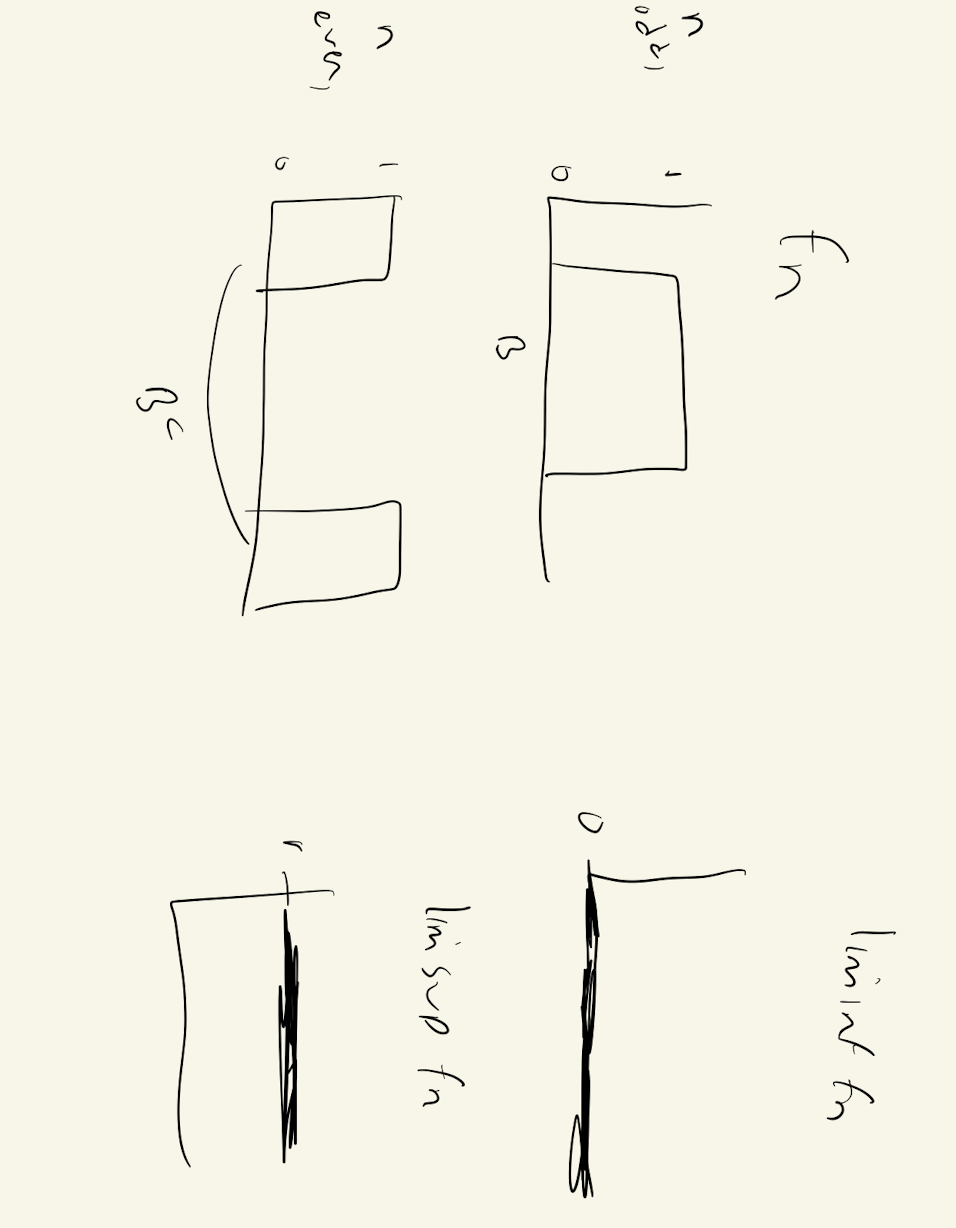
\includegraphics[width=.4\textwidth, angle=90]{images/fatous_lemma_example}	
 \end{figure}

 \begin{table}[htp!]
 \begin{tabular}{rl|l}
 & \textbf{Integrate first} & \textbf{Asymptotics first} \\
 \hline 
\textbf{Observation} & $\dint f_n  \dmu = 
\begin{cases}
\mu(B), & \text{n odd} \\ 
\mu(B^c), & \text{n even} \\ 	
 \end{cases}$	 &  $\liminf_{n \to \infty} f_n =0$ \\
 & & $\limsup_{n \to \infty} f_n =1$\\
 & & \\
 %\hline 
\textbf{Implication} & $\liminf_{n \to \infty} \dint f_n \dmu = \mu(B^c)$ & $\dint \liminf_{n \to \infty} f_n \dmu = 0$ \\
& $\limsup_{n \to \infty} \dint f_n \dmu = \mu(B)$ & $\dint \limsup_{n \to \infty} f_n \dmu = \mu(\Omega)$ \\
 \end{tabular}
 \end{table}

And so we see that strict inequalities occur in the expanded view of Fatou's lemma, \eqref{eqn:fatous_lemma_big_picture_view}. 

\begin{align*}
\explaintermbrace{0}{\ds\int_\Omega \bigg( \liminf_{n \to \infty} f_n \bigg) \dmu}  < \explaintermbrace{$\mu(B^c)$}{\liminf_{n \to \infty} \dint_\Omega f_n \dmu} < \explaintermbrace{$\mu(B)$}{\limsup_{n \to \infty} \dint_\Omega f_n \dmu} <  \explaintermbrace{$\mu(\Omega)$}{\ds\int_\Omega \bigg( \limsup_{n \to \infty} f_n \bigg) \dmu}  
%\labelit \label{eqn:fatous_lemma_big_picture_view_applied_to_example_with_strict_inequalities}
\end{align*}
The example captures the fact that \textit{integrals of asymptotics give more extreme values than asymptotics of integrals}.

\end{example}

\begin{remark}{\remarktitle{Fatou's Lemma for series.}} In the special case where $\Omega = \set{1,2,3, ...}$, $\F=2^\Omega$ (i.e. all subsets of $\Omega$), and $\mu$ is the counting measure, Example~\ref{ex:integrals_as_sums} tells us that the integrals are series. That is, we can write $\sum_{k=1}^\infty x_k = \int f \wrt{\mu}$, where $f : \Omega \to \mathcal{X}$ maps $\omega_1, \omega_2, \hdots$ to $x_1, x_2, \hdots$. 

In this setting, the big picture conclusion of Fatou's lemma  \eqref{eqn:fatous_lemma_big_picture_view} specializes to: \textit{\sout{integrals} series of asymptotics give more extreme values than asymptotics of series \sout{integrals}}:
%
\begin{align} 
\sum_{k=1}^\infty  \liminf_{n \to \infty} x_{nk}  \leq \liminf_{n \to \infty} \sum_{k=1}^\infty  x_{nk} \leq  \limsup_{n \to \infty} \sum_{k=1}^\infty  x_{nk} \leq \sum_{k=1}^\infty  \limsup_{n \to \infty} x_{nk}   
\label{eqn:fatous_lemma_applied_to_series}
\end{align}

This observation will be useful when we discuss weak convergence.

\label{rk:fatous_lemma_for_series}
\end{remark}


\subsection{Dominated Convergence Theorem}

The dominated convergence theorem justifies exchanging integrals and limits.  We begin with a motivating example where the exchange is not warranted.

\begin{example}{\remarktitle{Example where limits and integrals cannot be exchanged.}} Let $f_n = \frac{1}{n} \indicate{[0,n]}$.  Then $\int_{\R} f_n = 1$ for all $n$, and so $\lim_{n \to \infty} \int_{\R} f_n =1$.  But the pointwise limit $f := \lim_{n \to \infty} f_n = 0 $ and so $\int_{\R} f = \int_{\R}  0 = 0$.  %Note that the conditions of the Dominated Convergence Theorem cannot be met; there cannot be an integrable $g$ such that $|f_n| \leq g$, since $\sup_n f_n = f$ (see Remark \ref{rk:when_upper_or_lower_bound_is_contained_in_the_set_itself}) and $f$ is not integrable.  

% Reference: https://tex.stackexchange.com/questions/169638/simple-characteristic-function-or-step-function-in-pgfplots
%https://ctan.math.washington.edu/tex-archive/graphics/pstricks/contrib/pst-plot/doc/pst-plot-doc.pdf
\begin{figure}[H]
\centering 
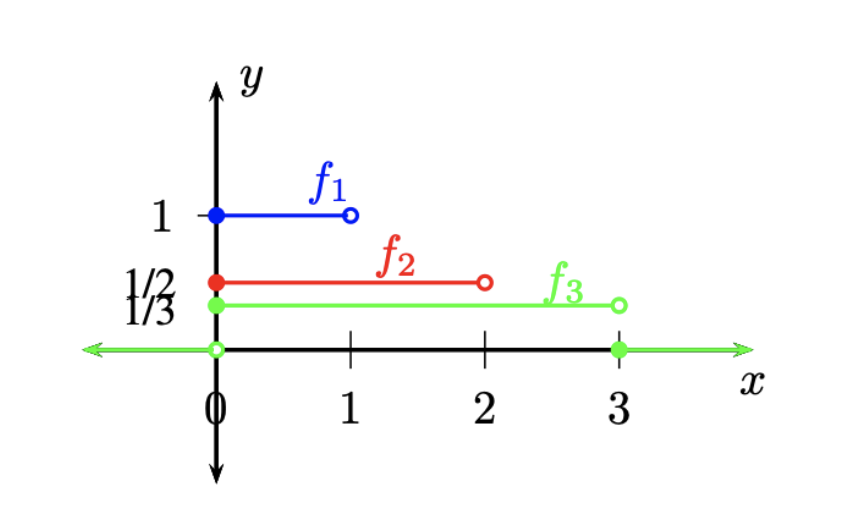
\includegraphics[width=.5\textwidth]{images/sequence_of_functions_where_limit_and_integral_cannot_be_exchanged}
\caption{The first 3 functions in a sequence $f_n$ where limit and integral (against Lebesgue measure) cannot be exchanged.}
% 
% Source code for making picture 
% \begin{pspicture}(-3.5,-1)(6,2)
% \psaxes[dx=1,Dx=1]{<->}(0,0)(-1,-1)(4,2)[$x$,-90][$y$,0]
%\rput(-0.5,0.5){\small 1/2}
%\rput(-0.5,0.3){\small 1/3}
%  
%%f_1
%%\psplot[linecolor=blue,arrows=<-o]{-3}{0}{0}
%\psplot[linecolor=blue,arrows=*-o]{0}{1}{1}
%%\psplot[linecolor=blue,arrows=*->]{1}{5}{0}
%\uput[0](.5,1.25){\blue{$f_1$}}
%%f_2
%%\psplot[linecolor=red,arrows=<-o]{-3}{0}{0}
%\psplot[linecolor=red,arrows=*-o]{0}{2}{.5}
%\uput[0](1,.7){\red{$f_2$}}
%%\psplot[linecolor=red,arrows=*->]{2}{5}{0}
%%f_3
%\psplot[linecolor=green,arrows=<-o]{-1}{0}{0}
%\psplot[linecolor=green,arrows=*-o]{0}{3}{.33}
%\uput[0](2.25,.5){\green{$f_3$}}
%\psplot[linecolor=green,arrows=*->]{3}{4}{0}
%\end{pspicture}
\end{figure}
\label{ex:a_sequence_where_limits_and_integrals_cannot_be_exchanged}
\end{example}

The dominated convergence theorem says that if all functions in a sequence are dominated by an integrable function ($|f_n| \leq g$), then the pathology of Example~\ref{ex:a_sequence_where_limits_and_integrals_cannot_be_exchanged} cannot happen, and limits and integrals can be safely exchanged. 



\begin{theorem}{\textbf{Dominated Convergence Theorem.}}. If $f_1,f_2,...,f,g$ are Borel measurable, $|f_n| \leq g$ for all $n$, where $g$ is $\mu$-integrable, and $f_n \to f$ a.e. $[\mu]$, then $f$ is $\mu$-integrable, and $\int_\Omega f_n \dmu \to \int_\Omega f \dmu$.
\label{thm:dominated_convergence}
\end{theorem}

\begin{proof}
We have $|f| \leq g$ a.e. {\tiny (In detail, $|f_n| \leq g$ can be unpacked into $f_n \leq g$ and $f_n \geq -g$.  Since limits preserve non-strict inequalities, we have ($f \leq g$ and $f \geq -g$) a.e.   So repacking the absolute value operator, the conclusion follows.)}, hence $f$ is integrable by Cor. \ref{cor:additivity_corollaries} (b).   

By hypothesis, both sides of the expanded Fatou's lemma apply, and so we have \eqref{eqn:fatous_lemma_big_picture_view}:

\begin{align*} 
\explaintermbrace{\tinycircled{1}}{\ds\int_\Omega \bigg( \liminf_{n \to \infty} f_n \bigg) \dmu}  \leq \explaintermbrace{\tinycircled{2}}{\liminf_{n \to \infty} \dint_\Omega f_n \dmu} \leq  \explaintermbrace{\tinycircled{3}}{\limsup_{n \to \infty} \dint_\Omega f_n \dmu} \leq \explaintermbrace{\tinycircled{4}}{\ds\int_\Omega \bigg( \limsup_{n \to \infty} f_n \bigg) \dmu}   
\end{align*}
But since $f_n \to f$ a.e, $\liminf_{n \to \infty} f_n = \limsup_{n \to \infty} f_n = \lim_{n \to \infty} f_n$ a.e., and so by the a.e. theorem (Thm. \ref{thm:almost_everywhere}), they have the same integrals: $\int_\Omega \liminf_{n \to \infty} f_n \dmu = \int_\Omega \limsup_{n \to \infty} f_n \dmu = \int_\Omega \lim_{n \to \infty} f_n \dmu $.   In other words, \tinycircled{1}=\tinycircled{4}, and so by sandwiching \tinycircled{2}=\tinycircled{3}.  Since the limit inferior and limit superior of the integrals are equal, the limit of the integrals exists as well, and all together we have
\[ \ds\lim_{n \to \infty} \dint_\Omega f_n \dmu = \dint_\Omega \ds\lim_{n \to \infty} f_n \dmu.\]
\end{proof}






\subsection{Continuity and differentiability of functions defined with an integral}

We now consider \textit{dependence on a parameter}.  Specifically, we consider integrals where the integrand depends on a real parameter.\footnote{Here, a ``parameter" refers to a variable in the domain of the function that is not integrated over.}  The following theorem describes continuity and the computation of derivative for such functions. 

\begin{theorem}{\textbf{Continuity and differentiability of functions defined with an integral.}}
Let 
%$f : \mathcal{X} \times [a,b] \to \R$, where $(-\infty < a < b < \infty)$.  
\begin{align*}
& f : \mathcal{X} \times [a,b] \to \R, && \text{ where } (-\infty < a < b < \infty) \\
& f(\cdot, t) : \mathcal{X} \to \R \text{ be integrable} && \forall t \in [a,b] \\
&F(t) := \ds\int_{\mathcal{X}} f(x,t) \dmu(x)  
\end{align*}
\begin{alphabate}
\item Suppose
\[ |f(x,t)| \leq g(x) \quad \quad \forall x,t \]
for some integrable $g$.   If $f(x,\cdot)$ is continuous for each $x$, then $F$ is continuous.
\item Suppose $\partial f / \partial t$ exists and 
\[ \bigg|\df{\partial f}{\partial t}(x,t)\bigg| \leq g(x) \quad \quad \forall x,t \]
for some integrable $g$.  Then $F$ is differentiable and 
\[ F'(t) = \ds\int_{\mathcal{X}} \df{\partial f}{\partial t}(x,t) \dmu(x) \]
\end{alphabate}
\label{thm:continuity_and_differentiability_of_functions_defined_with_an_integral}
\end{theorem}
	
\begin{proof}
\begin{alphabate}
\item We need to show that
\[ \ds\lim_{t \to t_0} f(x,t) = f(x,t_0) \implies  \ds\lim_{t \to t_0} F(t) = F(t_0)  \]	
So 
\begin{align*}
\ds\lim_{t \to t_0} F(t) &=   \ds\lim_{t \to t_0} \ds\int_{\mathcal{X}} f(x,t) \dmu(x) && \tinytext{definition of $F$}\\
&= \ds\int_{\mathcal{X}}  \ds\lim_{t \to t_0}  f(x,t) \dmu(x) && \tinytext{Dominated Convergence Thm}\\
&= \ds\int_{\mathcal{X}}  f(x,t_0) \dmu(x) && \tinytext{hypothesis}\\
&= F(t_0) && \tinytext{definition of $F$}
\end{align*}
\item First we note that $\frac{\partial f}{\partial t}$ is measurable.  This is true by the closure properties of measurable functions (Sec. \ref{sec:closure_properties_of_measurable_functions}), since
\[ \df{\partial f}{\partial t}(x,t_0) = \ds\lim_{n \to \infty} \explaintermbrace{$:=h_n(x)$}{\df{f(x, t_n) - f(x,t_0)}{t_n - t_0}} \]
for any sequence $\set{t_n}$ converging to $t_0$.

Next we note that $h_n(x)$ is bounded uniformly in $n$.  For all $n$, there is an $s_n$ between $t_0$ and $t_n$ such that
\[  |h_n| \stackexplain{(def)}{=} \bigg|\df{f(x, t_n) - f(x,t_0)}{t_n - t_0} \bigg| \stackexplain{(MVT)}{=} \bigg| \df{\partial f}{\partial t}(x,s_n) \bigg| \stackexplain{(hypothesis)}{\leq} g(x)\]
where MVT stands for the Mean Value Theorem.

Thus, we can apply the Dominated Convergence Theorem to $h_n$, i.e. $\lim_{n \to \infty} \int h_n(x) \dmu(x) = \int \lim_{n \to \infty} h_n(x) \dmu(x)$.  Using this, we obtain
\begin{align*}
F'(t_0) &= \ds\lim_{n \to \infty} \df{F(t_n) - F(t_0)}{t_n-t_0} && \tinytext{def. derivative} \\
&= \ds\lim_{n \to \infty }	\df{ \int f(x,t_n) \dmu(x)  - \int f(x,t_0) \dmu(x)}{t_n-t_0} && \tinytext{def. $F$} \\
&= \ds\lim_{n \to \infty }	\ds\int \df{ f(x,t_n)  -  f(x,t_0) }{t_n-t_0} \dmu(x) && \tinytext{linearity, applies since $f$ integrable} \\
&= \ds\int \df{\partial}{\partial t} f(x,t) \dmu(x) && \tinytext{Dominated Convergence Theorem, def. derivative}
\end{align*}

\end{alphabate}
	
\end{proof}

\begin{remark}{\remarktitle{Extensions to real-valued parameters with unbounded support.}}
Theorem \ref{thm:continuity_and_differentiability_of_functions_defined_with_an_integral}  may seem overly restrictive, since the real-valued parameter has bounded support.  However, as noted by \cite{folland1999real} pp. 56, continuity and differentiability are \textit{local} in nature.  Thus, if the hypotheses of (a) or (b) hold for all $[a,b] \subset I$ of an open interval $I$ (which is perhaps $\R$ itself), perhaps with the dominating function $g$ depending on $a$ and $b$, one obtains the continuity and differentiability of the integrated function $F$ on all of $I$! 	
\end{remark}


\section{$\S$ 1.7 Comparison of Lebesgue and Riemann integrals}

In this section, we show that integration with respect to Lebesgue measure is more general than Riemann integration, and we give a precise criterion for Riemann integration.

\paragraph{Review of Riemann integration.} Let $[a,b]$ be a bounded closed subset of the reals, and $f$ be a bounded real valued function on $[a,b]$. We assume $f$ is fixed throughout the discussion (i.e., we suppress dependence on $f$ in the notation).  Let $P: a=x_0 < x_1 < ... < x_n =b$ be a partition of $[a,b]$.  We construct the upper and lower sums as follows.  Let 
\begin{align*}
M_i &:= \sup \set{f(y) : x_{i-1} < y \leq x_i}, && i=1,...,n \\	
m_i &:= \inf \set{f(y) : x_{i-1} < y \leq x_i}, && i=1,...,n 
\end{align*}
And define step functions $\alpha$ and $\beta$, called the \textit{upper} and \textit{lower} functions for $f$ via 
\begin{align*}
\alpha(x) &= M_i && \text{ if } x_{i-1} < x \leq x_{i}   && i=1,...,n \\	
\beta(x) &= m_i && \text{ if } x_{i-1} < x \leq x_{i}  && i=1,...,n 	
\end{align*}
[$\alpha(a)$ and $\beta(a)$ may be chosen arbitrarily].   The upper and lower sums are defined as
\begin{subequations}
\begin{align}
U(P) &= \ds\sum_{i=1}^n M_i (x_i - x_{i-1}) \\	
L(P) &= \ds\sum_{i=1}^n m_i (x_i - x_{i-1}) 
\end{align}
\label{eqn:upper_and_lower_sums}	
\end{subequations}


Now let $P_1, P_2, ...$ be a sequence of partitions such that $P_{k+1}$ is a refinement of $P_k$ for each $K$, and such that $|P_k|$ (the length of the largest subinterval of $P_k$) approaches 0 as $k \to \infty$.  

If 
\begin{align}
 \lim_{k \to \infty} L(P_k) =  \lim_{k \to \infty} U(P_k) = r,
 \label{eqn:criterion_for_riemann_integrability}	
\end{align}
 independent of the particular sequence of partitions, then $f$ is said to be \textit{Riemann integrable} on $[a,b]$, and $r$ is the value of the \textit{Riemann integral}.\redfootnote{TODO: integrate this with my review of the Riemann integral in the appendix.} 

\paragraph{The criterion for Riemann integrability criterion in terms of Lebesgue integration.}

Now consider the measure space $(\Omega, \F, \mu) = ([a,b], \L([a,b]), \text{Lebesgue measure})$, where $\L([a,b])$ are the Lebesgue measurable sets (see Section \ref{sec:Lebesgue measurable sets}).  Let $P_k$ be a sequence of partitions described earlier, with $\alpha_k$ and $\beta_k$ the corresponding upper and lower functions.  Now since $\alpha_k$ and $\beta_k$ are simple functions, we can express the upper and lower sums \eqref{eqn:upper_and_lower_sums} as integrals with respect to Lebesgue measure $\mu$:
\begin{align*}
U(P_k) &= \ds\int_{[a,b]} \alpha_k \dmu \\
L(P_k) &= \ds\int_{[a,b]} \beta_k \dmu \\		
\end{align*}
Now we can bound the upper and lower functions by an integrable function. {\tiny (In detail, since we assumed $f$ is bounded,  we can write $|f| \leq M$, and therefore $|\alpha_k|,|\beta_k| \leq M$.  Moreover $M$ is integrable, since $\int_{[a,b]} M \dmu = M(b-a) < \infty$.)} Moreover, {\tiny (by Proposition \ref{prop:sup_and_inf_for_subsets_are_tighter})}, we have 
\[ \alpha_1 \geq \alpha_2 \geq ... \geq f \geq ... \geq \beta_2 \geq \beta_1 \]
so $\alpha_k$ and $\beta_k$ approach limit functions $\alpha$ and $\beta$.   Thus, we can apply Lebesgue dominated convergence theorem to obtain
\begin{align*}
\ds\lim_{k \to \infty} U(P_k) &= \ds\lim_{k \to \infty} \ds\int_{[a,b]} \alpha_k \dmu \stackexplain{(LDCT)}{=}  \ds\int_{[a,b]} \alpha \dmu  \\
\ds\lim_{k \to \infty} L(P_k) &= \ds\lim_{k \to \infty} \ds\int_{[a,b]} \beta_k \dmu \stackexplain{(LDCT)}{=}  \ds\int_{[a,b]} \beta \dmu   \\	
\end{align*}
Thus, we can write the criterion for Riemann integrability \eqref{eqn:criterion_for_riemann_integrability} in terms of the Lebesgue integral.  In particular, $f$ is Riemann integrable over $[a,b]$ with value $r$ iff 
\begin{align}
\ds\int_{[a,b]} \alpha \dmu = \ds\int_{[a,b]} \beta \dmu  = r
\label{eqn:criterion_for_riemann_integrability_in_terms_of_lebesgue_integral}
\end{align}
independent of the sequence of partitions $\set{P_k}$.


\paragraph{Continuity at a point as equality of the upper and lower functions.}  Here we provide a key observation which will help us to relate the Riemann integral and the Lebesgue integral. 

\begin{lemma}
If $x$ is not an endpoint of any subintervals of $P_k$, then 
\[ f \text{ is continuous at } x \quad \text{iff} \quad \alpha(x) = f(x) = \beta(x)\]	
\label{lemma:continuity_at_a_point_as_equality_of_upper_and_lower_functions}
\end{lemma}

\begin{proof}
\begin{itemize}
\item $\boxed{\implies}$.  $f$ is continuous at $x$ means that $\forall \epsilon>0, \exists \delta >0 :$
\begin{align*}
|y-x| < \delta \implies & |f(y) - f(x) | < \epsilon && \\
\implies &f(y) \leq f(x) + \epsilon  && \forall y \in B_x(\delta) \\ 
\implies &\sup_{y \in B_x(\delta)} f(y) \leq f(x) + \epsilon && \tinycircled{1}. 
\end{align*}
where $B_x(\delta)$ refers to a ball centered at $x$ with radius $\delta$.

Now let $I_k(x)$ be the subinterval in the $k$th partition to which $x$ belongs.  Since $|P_k| \to 0$, $|I_k(x)| \to 0$, and so
\[ \forall \delta>0, \exists K : \forall k \geq K, \quad  |y-x| < \delta \quad \forall y \in I_k(x) \quad \quad  \tinycircled{2} \]
Combining \tinycircled{1} and \tinycircled{2}, we obtain
\[ \forall \delta>0, \exists K : \forall k \geq K, \quad  \sup_{y \in I_k(x)} f(y) \leq f(x) + \epsilon \quad \quad  \tinycircled{3}\]
And of course, since the supremum is an upper bound and $x \in I_k(x)$, 
\[ \sup_{y \in I_k(x)} f(y) \geq f(x). \quad \quad  \tinycircled{4}\]
So combining \tinycircled{3} and \tinycircled{4}, and recalling that $\alpha_k(x) :=  \sup_{y \in I_k(x)} f(y)$, we have 
\[ \forall \delta>0, \exists K : \forall k \geq K, \quad  | \alpha_k(x) - f(x) | \leq  \epsilon\]
which is the definition of the limit.   That is,
\[ \ds\lim_{k \to \infty} \alpha_k(x) = f(x)\]
A similar argument holds for $\beta_k$.
\item $\boxed{\impliedby}$.  By hypothesis, 
\begin{align*}
\forall \epsilon>0, \exists K : \forall k \geq K, \\
 & | \sup_{y \in I_k(x)} f(y) - f(x) | \leq  \epsilon & \text{ and } && | \inf_{y \in I_k(x)} f(y) - f(x) | \leq  \epsilon  && \\	
 \stackrel{1}{\implies} & f(y) - f(x) < \epsilon & \text{ and } && f(y) - f(x) > -\epsilon && \forall y \in I_k(x) \\
\end{align*}
where (1) holds since the supremum is an upper bound and the infimum is a lower bound.  So 
\[ \forall \epsilon>0, \exists K : \forall k \geq K, \quad |f(y) - f(x) | < \epsilon \quad  \forall y \in I_k(x) \]
and taking $\delta$ to be the radius of $I_k(x)$, the definition of the continuity of $f$ at $x$ holds. 
\begin{figure}[H]
\centering
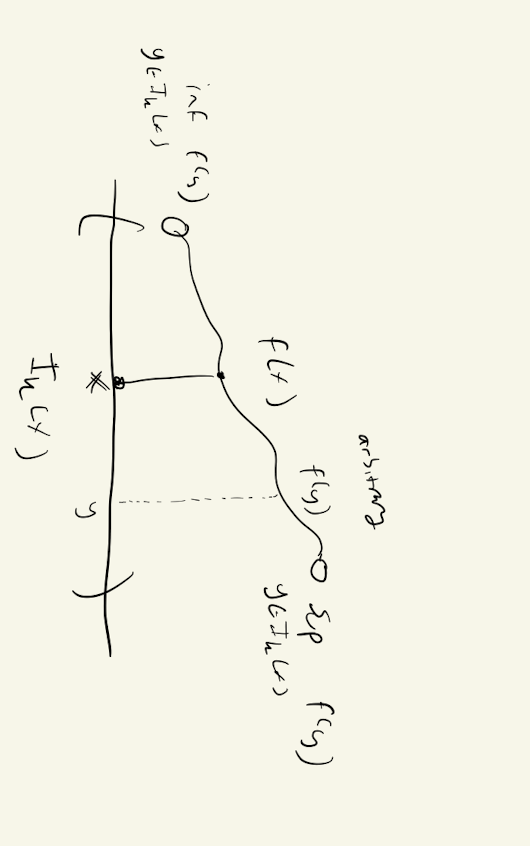
\includegraphics[width=.4\textwidth, angle=90]{images/continuity_from_equality_of_limits_of_upper_and_lower_functions}	
\end{figure}

\end{itemize}
\end{proof}

\paragraph{The theorem.}

\begin{theorem}
Let $f$ be a bounded real-valued function on $[a,b]$.	
\begin{alphabate}
\item The function $f$ is Riemann integrable on $[a,b]$ iff $f$ is continuous almost everywhere on $[a,b]$ (with respect to Lebesgue measure).
\item If $f$ is Riemann integrable on $[a,b]$, then $f$ is integrable with respect to Lebesgue measure on $[a,b]$, and the two integrals are equal.	
\end{alphabate}
\label{thm:relating_lebesgue_and_riemann_integrals}
\end{theorem}

\begin{proof}
\begin{alphabate}
\item
\begin{itemize}
\item $\boxed{\implies}$.  By \eqref{eqn:criterion_for_riemann_integrability_in_terms_of_lebesgue_integral}, if $f$ is Riemann integrable, then 
\[ \ds\int_{[a,b]} \alpha \dmu = \ds\int_{[a,b]} \beta \dmu = r\]
By linearity {\tiny (which holds immediately since $\alpha$, $\beta$ are integrable by the above equation; see Remark \ref{rk:additivity_holds_automatically_for_integrable_functions})}, 
\[  \ds\int_{[a,b]} (\alpha-\beta) \dmu =0  \]
Since $\beta \leq f \leq \alpha$ {\tiny (since each $\beta_k$ and $\alpha_k$ are lower and upper bounds by construction, and limits preserve non-strict inequalities)}, we have $\alpha-\beta \geq 0$, so by Theorem \ref{thm:properties_of_functions_derived_from_properties_of_integrals} (b), $\alpha-\beta =0$ a.e.  So {\tiny (by sandwiching)} $\alpha=\beta=f$ a.e.   So by Lemma \ref{lemma:continuity_at_a_point_as_equality_of_upper_and_lower_functions}, $f$ is continuous a.e.\footnote{Implicit in this last statement, I think, is that the endpoints are are set of measure 0, even in the limit.  If $E_k$ denotes the set of endpoints of the subintervals of $P_k$, and $E_{ik}$ denotes the $i$th such endpoint for $i=1,...,N_k$, then $\mu(\lim_{k \to \infty} E_k) \stackrel{1}{=} \lim_{k \to \infty} \mu(E_k) = \lim_k \mu(\cup_{i=1}^{N_k} E_{ik}) \stackrel{2}{=} 0$, where (1) holds by continuity of measure (from below; recall each successive partition is a refinement of the previous) and (2) holds since by additivity of measure, since each $E_{ik}$ is a singleton and the Lebesgue measure of any singleton is 0.
}
\item $\boxed{\impliedby}$.  By hypothesis and Lemma  \ref{lemma:continuity_at_a_point_as_equality_of_upper_and_lower_functions}, $\alpha = f = \beta$ a.e.   As a result, $f$ is measurable.   {\tiny ($\alpha, \beta$ are limits of simple functions, and hence measurable by closure properties of simple functions.  Thus, $f$ differs from a measurable function only on a subset of a set of measure 0.   Since the Lebesgue measurable sets $\L([a,b])$ are complete, $f$ must be measurable by Problem \ref{prob:in_a_complete_metric_space_you_are_a_measurable_function_if_you_are_equal_to_some_other_measurable_function_ae}.)}\footnote{After this line \cite{ash2000probability} also adds that $f$ is integrable. {\tiny (Since $f$ is bounded, say $|f| \leq L$, we have $\int_{[a,b]} f \dmu \leq \int_{[a,b]} L \dmu = L (b-a) < \infty $.) } But on my reading, we can just use the a.e. theorem directly after arguing that $f$ is measurable.} Since $\alpha=f=\beta$ a.e., by Theorem \ref{thm:almost_everywhere} (b),  we have
\begin{align}
\ds\int_{[a,b]} \alpha \dmu =  \ds\int_{[a,b]} f \dmu  = \ds\int_{[a,b]} \beta \dmu  
\label{eqn:lebesgue_integral_of_riemann_integral_fucntion_equals_the_lebesgue_integral_of_the_limits_of_the_upper_and_lower_functions}
\end{align}

Thus $f$ is Riemann integrable by \eqref{eqn:criterion_for_riemann_integrability_in_terms_of_lebesgue_integral}.\footnote{Presumably the ``independent of the sequence of partitions" condition of \eqref{eqn:criterion_for_riemann_integrability_in_terms_of_lebesgue_integral} is met here, since the argument -- in particular, Lemma  \ref{lemma:continuity_at_a_point_as_equality_of_upper_and_lower_functions} -- does not seem to depend on the sequence of partitions.}
\end{itemize}
\item If $f$ is Riemann integrable, then $f$ is continuous a.e. by part (a).   So \eqref{eqn:lebesgue_integral_of_riemann_integral_fucntion_equals_the_lebesgue_integral_of_the_limits_of_the_upper_and_lower_functions} holds.  Then, by \eqref{eqn:criterion_for_riemann_integrability_in_terms_of_lebesgue_integral}, $\int_{[a,b]} f \dmu = r$, the value of the Riemann integral. 
\end{alphabate}
\end{proof}

\section{\S 2.1 Signed measures} \label{sec:signed_measures}

This section plays the same role as Section 2.1 of \cite{ash2000probability}, although the primary reference here is Section 3.1 of \cite{folland1999real}.

\subsection{Overview of signed measures}



\begin{definition} Let $(\Omega,\F)$ be a measurable space.\footnote{Recall Definition \ref{def:measurable_space_and_measurable_sets}.}A \textbf{signed measure} on $(\Omega,\F)$ is a function $\nu : \F \to [-\infty, \infty]$ such that
\begin{itemize}
\item $\nu(\emptyset) = 0$;
\item $\nu$ assumes at most one of the values $\pm \infty$;
\item (\textit{countable additivity}) If $\set{A_j}$ is a sequence of disjoint sets in $\F$, then $\nu(\cup_{j=1}^\infty A_j) = \sum_{j=1}^\infty \nu(A_j)$.
\end{itemize}
\label{def:signed_measure}
\end{definition}

\begin{remark}
Every measure is a signed measure. 
\end{remark}

More generally, two mechanisms for forming signed measures come to mind:
\begin{enumerate}
\item $\nu = \mu_1 - \mu_2$, where $\mu_1$ and $\mu_2$ are measures on $\F$, and at least one measure is finite.
\item The set function defined by $\nu(A) = \int_A h \dmu$, where $h : \Omega \to [-\infty, \infty]$ is a measurable function such that at least one of $\int h^+ \dmu$ and $\int h^- \dmu$ is finite.  {\tiny (The function is defined $\forall A \in \F$ on measure space $(\Omega, \F, \mu)$.)}.
\end{enumerate}

\begin{remark}
\cite{folland1999real} points out that these are the \textit{only} two examples; every signed measure can be represented in either of these two forms.
\end{remark}


\begin{example}

We can define a signed measure on all subsets of the reals by the number of blue ticks minus the number of red ticks.\footnote{Note that even though \textit{Lebesgue measure} could not be defined on \textit{all} subsets of the reals, clearly other signed measures can be.   Recall from Remark \label{rk:implications_of_existence_of_set_that_is_not_Lebesgue_measurable} that the problem was translation invariance:  we showed that there cannot be a translation invariant measure that assigns a finite value to all intervals.  The (signed) measure in this example, however, is clearly not translation invariant.}
  
\begin{figure}[H]
\centering 
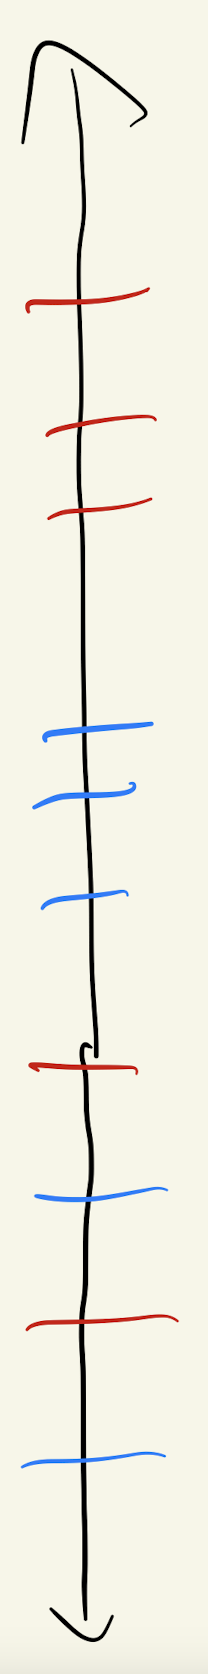
\includegraphics[width=.1\linewidth, angle=90]{images/signed_measure_example_with_ticks}
\end{figure}
\label{ex:a_signed_measure_with_ticks}
\end{example}


\begin{example}
We can define a signed measure on the reals by 
\[ \nu(A) := \ds\int_A |x| \dmu(x) \]
where $\mu$ is the Lebesgue measure.    To illustrate, compare the behavior of these set functions on two different sets:

\begin{tabular}{rcc}
& \multicolumn{2}{c}{Set} \\
Output & $[-5,-4]$ & $[-5,5]$\\	
$\mu$ & 1 & 10\\
$\nu$ & -1 & 0\\
\end{tabular}
 	
\end{example}


\begin{remark}
Signed measures are continuous by Theorem \ref{thm:continuity_of_countably_additive_set_functions} (continuity of countably additive set functions).
\end{remark}

\subsection{Hanh and Jordan Decompositions}

\begin{definition}
Given a signed measure $\nu$ on a measurable space $(\Omega, \F)$, a set $A \in \F$ is called
\begin{itemize}
\item \textbf{positive} if $\nu(B) \geq 0$ for all $B \subset A$.
\item \textbf{negative} if $\nu(B) \leq 0$ for all $B \subset A$.
\item \textbf{null}	if $\nu(B) = 0$ for all $B \subset A$.
\end{itemize}
\label{def:positive_negative_and_null_sets}
\end{definition}

\begin{remark}
To motivate Definition \ref{def:positive_negative_and_null_sets}, consider that unlike measures, \textit{signed} measures do not have the monotonicity property. So, for example, the condition $\nu(A)=0$ in isolation provides no information about the value of $\nu$ on subsets. For an illustration, recall  Example~\ref{ex:a_signed_measure_with_ticks}.
\end{remark}

\begin{theorem}{\textbf{The Hanh Decomposition Theorem}}
If $\nu$ is a signed measure on $(\Omega, \F)$, there exist a positive set $P$ and a negative set $N$ such that $\Omega = P \cupdot N$.  Moreover, if $P',N'$ is another such pair, then $P \triangle P' (= N \triangle N')$ is null for $\nu$.
\label{thm:hanh_decomposition}
\end{theorem}

\begin{proof}
See \cite{folland1999real} pp. 86.	
\end{proof}

\begin{example}
Let us consider two possible Hanh decompositions $(P,N), (P',N')$ for the signed measure of Example~\ref{ex:a_signed_measure_with_ticks}. The union of green intervals is a positive set $P$, and the union of orange intervals is a negative set $N$.  While there are a number of possible Hanh decompositions, these choices are ``not that different" from each other in the sense that for any two decompositions $(P,N), (P',N')$, the set $P \triangle P'$ (i.e. the set of points in exactly one version of green coloring), which equals $N \triangle N'$ (i.e. the set of points in exactly one version of orange coloring), is null for $\nu$. [In other words, the set of ``disagreement" is such that all subsets have signed measure 0.]  
\begin{figure}[H]
\centering 
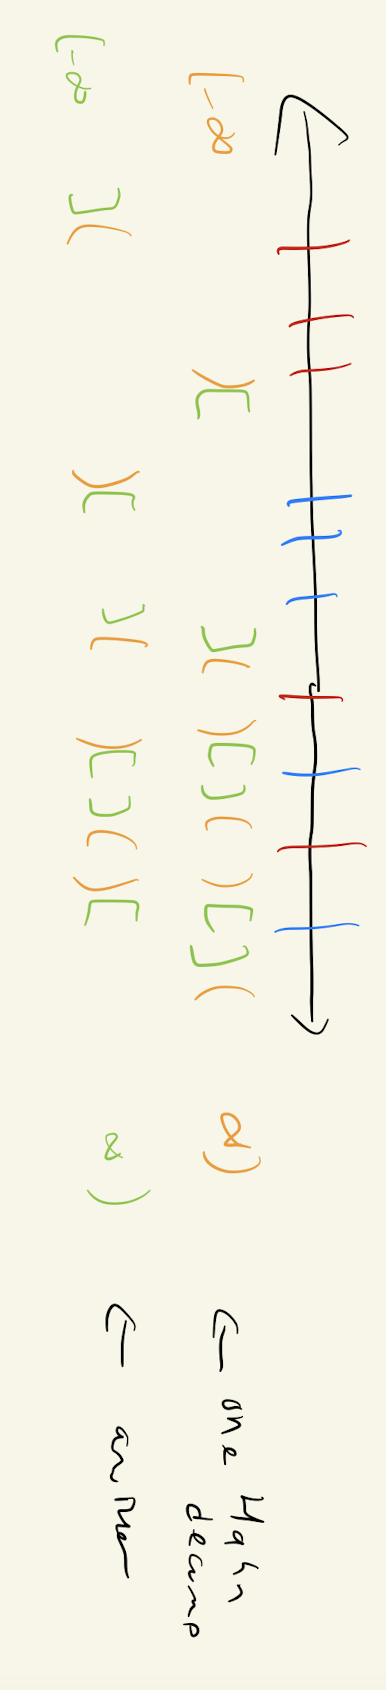
\includegraphics[width=.2\linewidth, angle=90]{images/hanh_decomposition_for_the_signed_measure_example_with_ticks}
\end{figure}
\label{ex:hanh_decomposition_for_the_signed_measure_example_with_ticks}
\end{example}


\begin{definition}
Let $\nu, \lambda$ be signed measures on a measurable space $(\Omega, \F)$.   Then $\nu$ and $\lambda$ are said to be \textbf{mutually singular}, written $\nu \perp \lambda$, if there exist $A,B \in \F$ such that $\Omega = A \cupdot B$ where $\nu$ is null for $A$ and $\lambda$ is null for $B$.
\label{def:mutually_singular}  
\end{definition}

So two signed measures are mutually singular if there is a partition of the universe into two cells such that each cell is null for a different signed measure.

\begin{example}
The normal distributions truncated to the positive reals ($\N_+$) and negative reals ($\N_-$) provide an example of mutually singular measures.  Note that in Definition \ref{def:mutually_singular}, we can take either $(A,B)=(\R_0^+,\R^-)$  or $(A'
,B')=(\R^+,\R_0^-)$, illustrating the non-uniqueness of the Hanh Decomposition.
\end{example}

Now we show that any signed measure can be expressed as the difference of two (latent) measures, which are moreover mutually singular. 

\begin{theorem}{\textbf{The Jordan decomposition theorem.}}
If $\nu$ is a signed measure, there exist unique measures $\nu^+$ and $\nu^-$ such that $\nu = \nu^+ - \nu^-$ and $\nu^+ \perp \nu^-$.
\end{theorem}

\begin{proof}
\begin{itemize}
\item \textit{Existence}.  Let $\Omega = P \cupdot N$ be a Hanh decomposition for $\nu$. {\tiny (So $\nu(A) \geq 0$ for all $A \subset P$ and  $\nu(B) \leq 0$ for all $B \subset N$)}. 

Define set functions $\nu^+$ and $\nu^-$ by:
\begin{align*}
\nu^+(E) &:= \nu(E \cap P) \\
\nu^-(E) &:= -\nu(E \cap N)
\end{align*}
which are both measures {\tiny (as they are non-negative and countably additive)}.  

Then:
	\begin{itemize}
	\item $\nu = \nu^+ - \nu^-$.  
	
	{\tiny This holds because E = $(E \cap P) \cupdot (E \cap N)$, so by countable additivity, $\nu(E) = \nu(E \cap P) + \nu(E \cap N) := \nu^+(E) - \nu^-(E)$. 
	}
	\item $\nu^+ \perp \nu^-$.
	
	{\tiny This holds because \begin{align*}
 		\nu^+(N) &= \nu(N \cap P) = \nu(\emptyset) =  0 \\
 		\nu^-(P) &= -\nu(P \cap N) = \nu(\emptyset) = 0,
 		\end{align*}
so $\Omega = P \cupdot N$ is the partition required for mutual singularity. (By monotonicity of measure, the equalities hold for subsets as well).}
	\end{itemize}

\item \textit{Uniqueness}.  TBD, or see \cite{folland1999real} pp. 87.	
\end{itemize}
	
\end{proof}

\begin{remark}
Don't let the notation confuse you.   Both $\nu^+$ and $\nu^-$ are (positive) measures.  The superscripts are meant to designate that $\nu^+$ is the minuend and  $\nu^-$  is the subtrahend in $\nu = \nu^+ - \nu^-$.	
\end{remark}


\subsection{Total Variation}

\begin{definition}
The \textbf{total variation} of a signed measure $\nu$, denoted $|\nu|$, is the measure given by 
\[ |\nu| := \nu^+ + \nu^- \]
\label{def:total_variation}	
\end{definition}

\begin{remark}
Definition \ref{def:total_variation} is well-defined because the sum of two measures is a measure:
\begin{itemize}
\item Non-negativity \checkmark 
\item Countable additivity \checkmark 

{\tiny Countable additivity holds because\footnote{TODO: Argue instead by appealing to a more general theorem.} 
\begin{align*}
|\nu|\bp{\bigcup_{i=1}^\infty A_i} &= \nu^+ \bp{\bigcup_{i=1}^\infty A_i}   + \nu^- \bp{\bigcup_{i=1}^\infty A_i}  \\
&= \ds\sum_{i=1}^\infty  \nu^+ (A_i) + \ds\sum_{i=1}^\infty  \nu^- (A_i) && \text{$\nu^+, \nu^-$ are measures} \\
&= \ds\sum_{i=1}^\infty \nu^+ (A_i) + \nu^-(A_i) && \text{Limits and sums commute; see \cite{strichartz2000way} Theorem 2.3.2 and apply it to partial sums} \\
&= \ds\sum_{i=1}^\infty |\nu|(A_i) && \text{def. of $|\nu|$}
\end{align*}

}	
\end{itemize}
	
\end{remark}

\begin{remark}{\remarktitle{An illustrative example of Hanh-Jordan Decomposition.}}
The picture below illustrates the structure of a signed measure $\nu$, as provided by a Jordan decomposition. As we will see in Problem \ref{prob:null_sets_are_those_with_zero_total_variation}, we can think about the ``set of disagreement" ( $P \triangle P' (= N \triangle N')$ ) between any two Hanh Decompositions ($(P,N), (P',N')$) as having a total variation $|\nu|$ of 0, so both $\nu^+$ and $\nu^-$ give zero measure to the sets of disagreement.
\begin{figure}[H]
\centering 
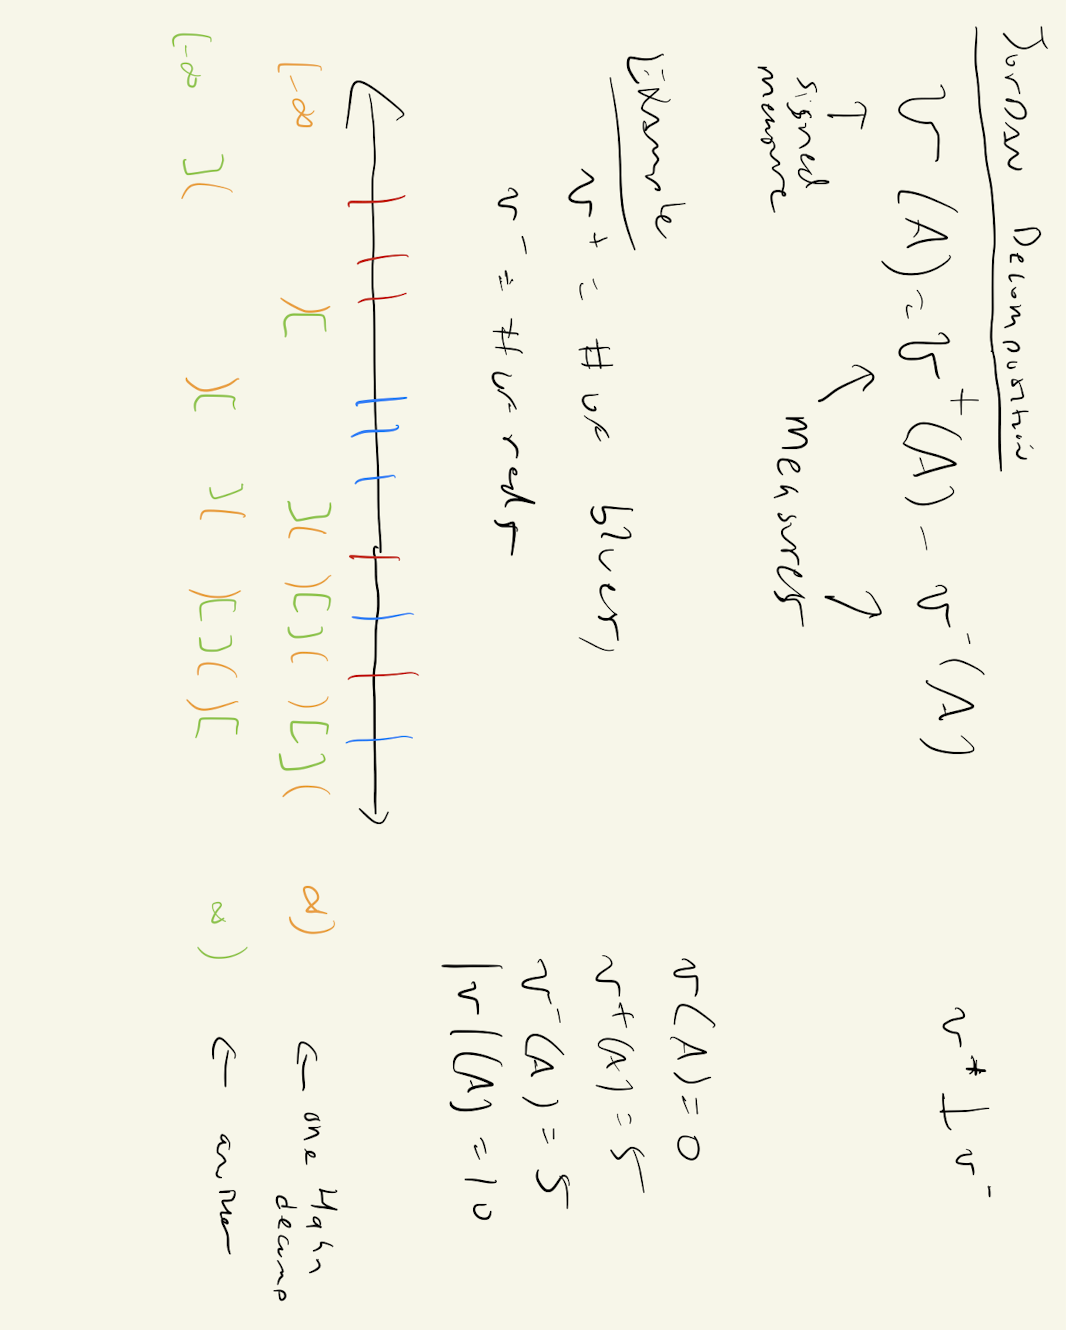
\includegraphics[width=.6\textwidth, angle=90]{images/hanh_jordan_decomp}
\end{figure}

\end{remark}

\begin{problem}{\remarktitle{Null sets are those with zero total variation.}}
Given a signed measure $\nu$ on a measure space $(\Omega,\F)$ and a set $E \in \F$, show that
\[ \text{$E$ is null for $\nu$}  \quad \text{iff} \quad |\nu|(E) = 0 \]	
\label{prob:null_sets_are_those_with_zero_total_variation}
\end{problem}

\begin{proof}[Solution.]
First recall the definitions
\begin{itemize}
\item 	$E$ is null for $\nu$: $\nu(F)=0 \quad  \forall F \subset E$.
\item  $|\nu|(E) = 0 $: $\nu^+(E) + \nu^-(E) = 0$.
\end{itemize}
Now the proof
\begin{itemize}
\item $\boxed{\implies}$.  Let $\Omega = P \cupdot N$ be a Hanh decomposition for $\nu$. 
Then 
\begin{align*}
\nu^+(E) &= \nu(E \cap P) = 0 \\
\nu^-(E) &= -\nu(E \cap N) = 0 
\end{align*}
where the first equalities are the Jordan decomposition, and the second equalities follow since $E$ is null for $\nu$ {\tiny (and $E \cap P, E \cap N \subset E$)}.

So 
\[  |\nu|(E) = \nu^+(E) + \nu^-(E) = 0. \]
\item $\boxed{\impliedby}$.	
\begin{align*}
|\nu|(E) = 0 & \iff  \nu^+(E) + \nu^-(E) =0 && \tinytext{def. $|\nu|$} \\
&\implies \nu^+(E) = 0, \nu^-(E) = 0 && \tinytext{non-negativity of measure} \\
&\implies \nu^+(F) = 0, \nu^-(F) = 0  \quad \forall F \subset E && \tinytext{monotonicity of measure}	\\
& \implies  \nu^+(F) + \nu^-(F) =0 \quad \forall F \subset E && \\
&\implies \nu(F) = 0 \quad \forall F \subset E && 
\end{align*}

\end{itemize}

\end{proof}


\subsection{Integrating against signed measure}

 We can define integration against a signed measure $\nu$ in terms of integrals against measure by using the Jordan decomposition $\nu = \nu^+ - \nu^-$.  

\begin{definition}{\textbf{Integration against signed measure}}
Let $\nu$ be a signed measure and let $f$ be a Borel measurable function.  Then we define
\begin{align}
\int f \, d\nu :=  \int f \, d\nu^+ - \int f \, d\nu^-
\label{eqn:integration_against_signed_measure}
\end{align}

\label{def:integration_against_signed_measure}
\end{definition}

The integral is finite if both $\int f d\nu^+$ and $\int f d\nu^+$ are finite. 




\section{\S 2.2 Lebesgue-Radon-Nikodym Theorem}

This section plays the same role as Section 2.2 of \cite{ash2000probability}, although the primary reference here is Section 3.2 of \cite{folland1999real}.

\subsection{Absolute continuity} \label{sec:absolute_continuity}

In this section, we define absolute continuity and give some useful properties.

\begin{definition}
Let $\nu$ be a signed measure and $\mu$ a measure on a measurable space $(\Omega, \F)$.  We say that $\nu$ is \textbf{absolutely continuous} with respect to $\mu$, and write
\[ \nu \ll \mu \]
if 
\[ \mu(A) = 0 \implies \nu(A) = 0 \quad \forall A \in \F. \]
\label{def:absolute_continuity}	
\end{definition}

\begin{example}

Below we give examples.  For these examples, let $(\Omega, \F) = (\R, \B(\R))$.

\ifActive
\textbf{Workshop Discussion:} Can you think of any examples?
\else 
	\begin{enumerate}
	\item Let $\mu$ be a univariate Gaussian and $\nu$ be a Gaussian that is truncated (e.g. to the set of positive reals).  Then $\nu \ll \mu$ but $\mu \not\ll \nu$.
	\item Let $\mu$ be Lebesgue measure and $\nu$ give the number of integers in a set.  Then $\nu \not\ll \mu$ and $\mu \not\ll \nu$.
	\item Let $\mu$ be Lebesgue measure and $\nu$ be twice Lebesgue measure.  Then $\nu \ll \mu$ and $\mu \ll \nu$.
	\end{enumerate}
\fi 
\label{ex:examples_with_absolute_continuity}
\end{example}


\begin{remark}{\remarktitle{Indefinite integrals are absolutely continuous.}}

Let $\nu$ be an ``indefinite integral" with respect to $\mu$.\footnote{This interpretation of ``indefinite integral" is used in \cite[pp.~61]{ash2000probability}.}
\[ \text{ i.e. } \; \nu(A) = \ds\int_A h \dmu, \quad \quad \forall A \in \F \]

Then $\nu \ll \mu$
\[ \text{ i.e. } \; \mu(A) = 0 \implies \nu(A) = 0  \quad \quad \forall A \in \F \]
\label{rk:indefinite_integrals_are_absolutely_continuous}
\end{remark}

\begin{proof}\footnote{My first attempt at a proof worked through the definition for Lebesgue integral, working up from simple functions to non-negative to arbitrary functions.  However, the proof we provide here, which uses the strategy in Section 2.2 of \cite{ash2000probability}, is much nicer.  Note that my original strategy of proving via the definition just basically recapitulates the proof of Theorem \ref{thm:almost_everywhere} (a), so we might as well rely on the Theorem to do that dirty work.}

\ifActive
\textbf{Workshop Exercise: Prove this.}
\else 
	If $\mu(A) =0$, $h \indicate{A} = 0$ a.e.  So by Theorem \ref{thm:almost_everywhere} (a), 
	\[ \ds\int_A h \dmu = 0 \]
\fi 
\end{proof}

\begin{remark}{\remarktitle{Radon-Nikodym as a converse.}}
The Radon-Nikodym theorem is an assertion in the opposite direction of Remark \ref{rk:indefinite_integrals_are_absolutely_continuous}:  if $\nu \ll \mu$ (and $\mu$ is $\sigma$-finite on $\F$), then $\nu$ is an indefinite integral with respect  to $\mu$. 
\end{remark}


\begin{remark}{\remarktitle{A signed measure is absolutely continuous iff its total variation is absolutely continuous.}}\footnote{This is \cite{folland1999real} Problem 3.2.8a}
Let $\nu$ be a signed measure and $\mu$ a measure on a measurable space $(\Omega, \F)$.  Then 
\[ \nu \ll \mu \quad \text{iff} \quad |\nu| \ll \mu \]
\label{rk:signed_measure_is_absolutely_continuous_iff_its_total_variation_is_absolutely_continuous}
\end{remark}

\begin{proof}
Using the Jordan decomposition and the definitions (of absolute continuity and total variation), we write the following for reference:
\begin{align*}
\nu \ll \mu &\; \text{ means}  \\
&\mu(A) = 0 \implies \nu(A) = 0 \\
& \quad \text{ i.e. } \nu^+(A) - \nu^-(A) = 0 \\
|\nu| \ll \mu &\; \text{ means}  \\
&\mu(A) = 0 \implies |\nu|(A) = 0 \\
& \quad \text{ i.e. } \nu^+(A) + \nu^-(A) = 0 \\
\end{align*}
for all $A \in \F$.

And now we proceed:
\begin{itemize}
\item $\boxed{\impliedby}$. The hypothesis plus non-negativity implies
\[ \nu^+(A), \; \nu^-(A) =0 \]
\item $\boxed{\implies}$. 
\[ \begin{array}{rcl}
\mu(A) = 0  &\stackexplain{monotonicity}{\implies} & A \text{ is $\mu$-null } \\
&& \quad \text{ i.e. } \mu(B)=0 \quad \forall \, B \subset A \\
& \stackexplain{hypothesis}{\implies} &  \nu(B) = 0 \quad \forall \, B \subset A \\
& \stackexplain{null sets have zero total variation (Problem \ref{prob:null_sets_are_those_with_zero_total_variation}) }{\implies}& |\nu|(A) = 0  
\end{array}
\] 

%\end{array}

\end{itemize}

\end{proof}

\begin{remark}{\remarktitle{Absolute continuity is the antithesis of mutual singularity.}}

This statement (from \cite{folland1999real}) captures the fact that 
%
\[ \begin{array}{rl}
\text{ if } & \nu \text{ is a signed measure } \\
   & \mu \text{ is a measure } \\
   & \nu \ll \mu \\
   & \nu \perp \mu \\
\text{ then } & \nu \equiv 0
\end{array}
\]
%

	
\label{rk:absolute_continuity_is_the_antithesis_of_mutual_singularity}
\end{remark}

\begin{proof}
First recall
\[ \nu \ll \mu \stackexplain{Remark~\ref{rk:signed_measure_is_absolutely_continuous_iff_its_total_variation_is_absolutely_continuous}}{\iff} |\nu| \ll \mu \]
Now by mutual singularity
\[
\begin{array}{rlclcl}
\exists A,B \in \F: & \Omega = A \cupdot B && \\
& \nu \text{ is null for } A & \stackexplain{Problem \ref{prob:null_sets_are_those_with_zero_total_variation}}{\iff}& |\nu|(A) = 0\\ 
& \mu \text{ is null for } B & \stackexplain{special case}{\implies}& \mu(B) = 0 & \stackexplain{$|\nu| \ll \mu$}{\implies} & |\nu|(B) = 0\\ 
\end{array}
\]

So 
\begin{align*}
|\nu|(\Omega) & \stackexplain{countable additivity}{=} |\nu|(A) + |\nu|(B)  \stackexplain{see above}{=}  0 	 \\
& \stackexplain{monotonicity, since $|\nu|$ is a measure}{\implies} |\nu| \equiv 0 \\
& \stackexplain{*}{\implies} \nu \equiv 0.
\end{align*}
{\tiny Implication (*) holds since 
\begin{align*}
|\nu| \equiv 0 & \stackexplain{def}{\iff} \nu^+ + \nu^- \equiv 0 \\
& \stackexplain{non-negativity}{\implies} \nu^+  \equiv 0, \nu^- \equiv 0 \\
& \implies \nu^+ - \nu^- \equiv 0 \\
& \stackexplain{def.}{\iff} \nu \equiv 0.
\end{align*}
}

\end{proof}

We now provide some motivation for the name ``absolute continuity".

\begin{theorem}{\textnormal{(Name-justifying characterization of absolute continuity.)}}
Let $\nu$ be a finite signed measure and $\mu$ a positive measure on $(\Omega, \F)$.  Then 


\[
\begin{array}{lcr}	
\nu \ll \mu  & \text{iff} &  \forall \epsilon > 0, \; \exists \delta > 0 : \forall A \in \F, \\
(\text{i.e. } \mu(A) = 0 \implies \nu(A) = 0) & & \mu(A) < \delta \implies |\nu(A)| < \epsilon \\
\tinycircled{A} & & \tinycircled{B} 
\end{array}
\]	
\label{thm:justifying_the_name_absolutely_continuous}
\end{theorem}

\begin{proof}
\begin{itemize}
\item $\boxed{\impliedby}$. 
\[  \mu(A) = 0 \implies \mu(A) < \delta \quad \forall \delta \stackexplain{hypothesis}{\implies} |\nu(A)| < \epsilon \quad \forall \epsilon \implies \nu(A) = 0\]
\item $\boxed{\implies}$.   We proceed by contraposition. Since not \tinycircled{B},
\[
\begin{array}{lcrr}
\exists \epsilon > 0 : & \forall n \in \mathbb{N}, &  \exists A_n \in \F : & \\
\mu(A_n) \leq 2^{-n} & \text{ but } & |\nu|(A_n) \stackexplain{*}{\geq} |\nu(A_n) | \geq \epsilon 
& \quad \tinycircled{+} \end{array}
\]
where in Equation (*), we move work with $|\nu|$ since it is a measure.

{\tiny The inequality holds since  
\begin{align*}
|\nu(A)| &	\leq |\nu|(A) \\
|\nu^+(A) - \nu^-(A)| &\leq |\nu^+(A) + \nu^-(A)| \\
| x -y | &\leq |x + y|
\end{align*}
where we have applied the Jordan decomposition and properties of real numbers.
}

To show \tinycircled{A}, recall from Remark \ref{rk:signed_measure_is_absolutely_continuous_iff_its_total_variation_is_absolutely_continuous} that $\nu \ll \mu$ iff $|\nu| \ll \mu$, so
\[  \text{N.T.S.} \quad  \exists B \in \F : \; \mu(B) = 0 \quad \text{but} \quad |\nu|(B) \neq 0 \]
Let $B_k = \cup_{n=k}^\infty A_n, \; B = \cap_{k=1}^\infty B_k$.  So 
\[  B = \limsup A_n = \set{x : x \in A_n \text{ i.o. }}\]
Then by the Borel-Cantelli Lemma (Lemma \ref{lemma:borel_cantelli}), $\mu(B)=0$.  But 
\[ |\nu|(B) \stackexplain{cty from above}{=} \ds\lim_{k \to \infty} |\nu| (B_k) \stackexplain{monotonicity, \tinycircled{+}}{\geq} \ds\lim_{k \to \infty} \epsilon = \epsilon.  \]
where continuity from above holds because $B_k$ are decreasing, and $|\nu|(B_1)$ is finite because $\nu$ finite $\implies |\nu|$ finite.

{\tiny In fact $\nu$ finite $\iff |\nu|$ finite. This  can be seen by appealing to the  Jordan decomposition of $\nu$ and the definition of $|\nu|$.  For any $E \in \F$, 
\begin{align*}
\nu(E) &= \nu^+(E) - \nu^-(E) \not\in \set{\infty, -\infty}\\
\iff &\\
|\nu|(E) &= \nu^+(E) + \nu^-(E) \not\in \set{\infty, -\infty}.
\end{align*}
%
Both statements say that the two numbers $\nu^+(E), \nu^-(E)$ are both finite.}
\end{itemize}	
\end{proof}

As a corollary, we have that an integral of any (integrable) function over a set can be made arbitrarily small if the measure of the set is sufficiently small.

\begin{corollary}
Let $f$ be an integrable function with respect to $\mu$. Then $\forall \epsilon > 0, \; \exists \delta > 0$ such that 
\[  \mu(A) < \delta \implies \bigg| \int_A f \wrt{\mu} \bigg| < \epsilon \]	
\end{corollary}

\begin{proof}
By Theorem \ref{thm:integrals_are_countably_additive_set_functions}, the set function $\nu : \F \to \overline{\R}$ defined by $\nu(A) = \int_A f \wrt{\mu}$ is a signed measure.    Moreover, $\nu \ll \mu$, since indefinite integrals are absolutely continuous (see Remark \ref{rk:indefinite_integrals_are_absolutely_continuous}).  Thus, the implication follows from the name-justifying characterization of absolute continuity (Theorem \ref{thm:justifying_the_name_absolutely_continuous}). 
\end{proof}

\subsection{The theorem}

\begin{lemma}
Let $\nu, \mu$ be a finite  measures on $(\Omega, \F)$.  Then either $\nu \perp \mu$ or there exist $\epsilon > 0$ and $A \in \F$ such that $\mu(A) > 0$ and $\nu \geq \epsilon \mu$ on $A$.
\label{lemma:lemma_for_lebesgue_radon_nikodym}
\end{lemma}

\begin{proof}
See \cite[pp.~89]{folland1999real}.
\end{proof}


\begin{theorem}{\textbf{The Lebesgue-Radon-Nikodym Theorem.}} Let $\nu$ be a $\sigma$-finite signed measure and $\mu$ a $\sigma$-finite (positive) measure on $(\Omega, \F)$.  There exist unique $\sigma$-finite signed measures $\lambda, \rho$ on $(\Omega, \F)$ such that
\[ \nu = \lambda + \rho, \quad \text{ where } \quad \lambda \perp \mu \quad \text{ and } \quad \rho \ll \mu\]
Moreover, there is an extended $\mu$-integrable function $f : \Omega \to \R$ such that $d\rho = f \, d\mu$, and any two such functions are equal $\mu$-a.e.
\label{thm:lebesgue_radon_nikodym}
\end{theorem}


\begin{proof}
We prove the theorem in the special case that $\nu$ and $\mu$ are finite (positive) measures.  For a full proof, see \cite[pp.~90]{folland1999real}.
	
Let 
\[ \mathcal{S} := \biggset{ f : \Omega \to [0,\infty] : \ds\int_E f \, d\mu \leq \nu(E) \quad \forall E \in \F}\]
$\mathcal{S}$ is nonempty since $0 \in \mathcal{S}$.  Now if $f,g \in \mathcal{S}$, then $h:=\max(f,g) \in \mathcal{S}$, because if $A:=\set{x: f(x) > g(x)}$, then for any $E \in \F$, we have
\begin{align*}
\ds\int_E h \dmu = \ds\int_\Omega \indicate{E} h \dmu &= \ds\int_\Omega \bigg( \indicate{E \cap A} + \indicate{E \cap A^c}  \bigg) h \dmu  \\
&= \ds\int_{E \cap A} h \dmu +  \ds\int_{E \cap A^c} h \dmu \\
&= \ds\int_{E \cap A} f \dmu +  \ds\int_{E \cap A^c} g \dmu \\
& \stackexplain{(since $f,g \in \mathcal{S}$)}{\leq} \nu(E \cap A) + \nu(E \cap A^c) \\
& \stackexplain{countable additivity}{=} \nu(E). 
\end{align*}

Now let $a:=\sup \set{\int_\Omega f \dmu : f \in \mathcal{S}}$, and note that $a \stackexplain{sup is LUB}{\leq} \nu(\Omega) \stackexplain{assumption}{<} \infty$.  By a property of the supremum (see Remark~\ref{rk:existence_of_sequences_converging_to_infimum_and_supremum}), we can find a sequence $\set{f_n} \in \mathcal{S}$ such that $\int_\Omega f_n \dmu \to a$.  Now if we let $g_n := \max (f_1,\hdots, f_n)$, then $g_n \in \mathcal{S}$ by applying induction, since we have shown that $\mathcal{S}$ is closed under the maximum operator. It follows that $\int_\Omega g_n \dmu \to a$.

{\tiny 
Let us show that $\ds\lim_{n \to \infty} \int_\Omega g_n \dmu = a$.

\begin{itemize}
\item $\boxed{\geq}$.
\begin{align*}
\int_\Omega g_n \dmu &\geq \int_\Omega f_n \dmu && \text{by monotonicity of integral} \\
\implies \ds\lim_{n \to \infty} \int_\Omega g_n \dmu &\geq \ds\lim_{n \to \infty}  \int_\Omega f_n \dmu  = a && \text{limits preserve non-strict inequalities}
\end{align*}

\item 	$\boxed{\leq}$. Since $g_n \in \mathcal{S}$,
\begin{align*}
\int_\Omega g_n \dmu &\leq a && \text{supremum is upper bound} \\
\implies \ds\lim_{n \to \infty} \int_\Omega g_n \dmu &\leq a && \text{limits preserve non-strict inequalities}
\end{align*}
\end{itemize}
}

Since $g_n$ is an increasing sequence, there exists a function $f : \Omega \to [0,\infty]$ such that $g_n \uparrow f$ (see Prop.~\ref{prop:limit_of_an_increasing_sequence_of_functions_exists_and_is_the_supremum_if_we_allow_functions_to_map_to_the_extended_reals}),\redfootnote{TODO: Show specifically that $f = \sup_n f_n$. The proposition gives us that $g = \sup_n g_n = \sup_n \max_{m \leq n} f_n$.} and by monotone convergence theorem
\[ \ds\int_\Omega f \dmu = \ds\lim_{n \to \infty} \ds\int_\Omega g_n \dmu = a < \infty  \]
So $f < \infty$ a.e. (by Theorem~\ref{thm:properties_of_functions_derived_from_properties_of_integrals} a), and so we may take $f$ to be real-valued everywhere. 

Now define $\rho$ by $\rho(A) = \int_A f \dmu$, and define $\lambda := \nu-\rho$.  {\tiny (In differential notation, we can express both conditions simultaneously via $d\lambda = d\nu - f d\mu$.) }  Then the existence conditions of the theorem hold:
\begin{itemize}
\item $\nu = \lambda + \rho$? \greencheck  {\tiny Addition.} 
\item $\rho \ll \mu$? \greencheck  {\tiny This holds because indefinite integrals are absolutely continuous (see Remark \ref{rk:indefinite_integrals_are_absolutely_continuous}).}
\item $\lambda \perp \mu$? \greencheck  {\tiny First note $\lambda \geq 0$ since $f \in \mathcal{S}$.  So we proceed via Lemma~\ref{lemma:lemma_for_lebesgue_radon_nikodym}.  BWOC, suppose not $\lambda \perp \mu$. Then there is $\epsilon >0, A \in \F : \mu(A) >0$ and $\lambda \geq \epsilon \mu$ on $A$.   Now
\begin{align*}
\lambda & \geq \indicate{A} \epsilon \mu && \tinytext{by hypothesis, and $\lambda \geq 0$} \\
\implies d\nu - f \, \dmu & \geq \epsilon \indicate{A} \dmu && \tinytext{by def. $\lambda$, differential notation} \\ 
\implies d\nu & \geq (f+\epsilon \indicate{A}) \dmu && \tinytext{addition} \\
\implies (f+\epsilon \indicate{A}) & \in \mathcal{S} && \tinytext{by def. $\mathcal{S}$}
\end{align*}

But by linearity {\tiny (which applies immediately since $(f+\epsilon \indicate{A})$ is integrable)}, we have
\[ \ds\int_\Omega (f+\epsilon \indicate{A}) \dmu = a + \epsilon \mu(A) > a,\]
which contradicts the definition of the supremum.
}
\end{itemize}

Now we show uniqueness.
\[ \begin{array}{rl}
\text{We have} & d\nu = d\lambda + f d\mu \\
\text{Suppose also} & d\nu = d\lambda' + f' d\mu
\end{array}
\]
Then
\[ \begin{array}{lrlr}
 & d\lambda - d\lambda' &=  (f-f') d\mu &\\
\text{But} & \lambda - \lambda' & \perp \mu & \tinytext{Justified below} \\
\text{And} & \lambda - \lambda' & \ll \mu & \tinytext{Since $d(\lambda - \lambda') = (f-f')\dmu$ ; indefinite integrals are absolutely continuous (Remark \ref{rk:indefinite_integrals_are_absolutely_continuous})} \\
\text{So} & \lambda-\lambda' &=0 & \tinytext{$\ll$ and $\perp$ are antitheses; see Remark~\ref{rk:absolute_continuity_is_the_antithesis_of_mutual_singularity}}\\
\text{So} & \lambda&=\lambda' &\\
\text{So} & f&=f' \quad [\mu]-a.e. &  \tinytext{Cor.~\ref{cor:equal_integrals_for_all_measurable_sets_implies_the_functions_are_equal_ae}}
\end{array}
\]

{\tiny 
Let us show that if $\lambda_1 \perp \mu$ and $\lambda_2 \perp \mu$, then $\lambda_1  - \lambda_2 \perp \mu$.

\[ 
\begin{array}{rcl}
\lambda_1 \perp \mu & \text{means} & \exists E_1, F_1 : E_1 \cupdot F_1 = \Omega \\
& & E_1 \text{ null for } \lambda_1 \\
& & F_1 \text{ null for } \mu  \\
\lambda_2 \perp \mu & \text{means} & \exists E_2, F_2 : E_2 \cupdot F_2 = \Omega \\
& & E_2 \text{ null for } \lambda_2 \\
& & F_2 \text{ null for } \mu  \\
\end{array}
\]
Now let $\lambda = \lambda_1 - \lambda_2$.
\[ 
\begin{array}{rl}
\text{Let} & E = E_1 \cap E_2 \\
& \text{Then $E$ null for $\lambda_1$ and $\lambda_2$, so $E$ null for $\lambda = \lambda_1 - \lambda_2$} \\
\text{Let} & F := E^c = (E_1 \cap E_2)^c = E_1^c \cup E_2^c = F_1 \cup F_2 \\
& \text{So $F$ null for $\mu$}.
\end{array}
\]
}

  
\end{proof}


\subsection{Focus on Radon-Nikodym}


\begin{corollary}{\textbf{Radon-Nikodym Theorem.}}
Let $\nu$ be a $\sigma$-finite signed measure and $\mu$ a $\sigma$-finite (positive) measure on $(\Omega, \F)$.  Let $\nu \ll \mu$. Then $d \nu = f d\mu$ for some (extended $\mu$-integrable) function $f: \Omega \to \R$. In other words,
\begin{align}
 \nu(A) = \ds\int_A f \wrt{\mu} \quad \text{ for all } \quad A \in \F 
 \label{eqn:radon_nikodym}	
\end{align}
\label{cor:radon_nikodym}
\end{corollary}

\begin{proof}
In the Lebesgue-Radon-Nikodym theorem, set $\rho=\nu$ and $\lambda=0$.	
\end{proof}


\begin{terminology}
We refer to $f$ in \eqref{eqn:radon_nikodym} as the \textbf{Radon-Nikodym derivative} or \textbf{density} of $\nu$ with respect to $\mu$.   We denote it by $d\nu/d\mu$.  (Strictly speaking, $d\nu/d\mu$ should be construed as a class of functions equal to $f$ $\mu$-a.e.). When $\mu$ is the Lebesgue measure, then $f$ is often simply called the density of $\nu$.
\end{terminology}

Below we note that in the special case where $\nu$ is a measure, the Radon-Nikodym derivative must be non-negative almost everywhere. (Hence, it can be taken to be non-negative everywhere.)
 
\begin{corollary}
Let the hypotheses of the Radon-Nikodym Theorem (Cor.~\ref{cor:radon_nikodym}) hold.  If $\nu \geq 0$, then $f \geq 0$ a.e. $[\mu]$. 
\end{corollary}

\begin{proof}
Let $A := \set{x : f(x) < 0}$.  Now 
\[ 0 \stackexplain{measure}{\leq} \nu(A) = \int_A f \dmu \stackexplain{monotonicity}{\leq} 0 \]
So $\int_A f \dmu =0$.  Negating this and applying the scalar multiple property, we have that a non-negative function integrates to zero :  $\int - f \indicate{A} \dmu =0$.  Thus, by Theorem~\ref{thm:properties_of_functions_derived_from_properties_of_integrals} b), the integrand $- f \indicate{A} =0$ a.e. $[\mu]$, and so negating again, $f \indicate{A} =0$ a.e. $[\mu]$.  But by construction, $f < 0$ on $A$, so $\mu(A)=0$.
\end{proof}


%As pointed out by \cite[pp.91]{folland1999real}, the formulas suggested by the differential notation $d\nu/d\mu$ generally apply. For example, $d(\nu_1 + \nu_2)d\mu = d\nu_1/d\mu + d\nu_2/d\mu$.  Additionally, the Radon-Nikodym derivative satisfies a chain rule. 

\begin{proposition}{\remarktitle{Calculus with Radon-Nikodym Derivatives.}}\footnote{The terminology is borrowed from \url{https://pages.stat.wisc.edu/~doksum/STAT709/n709-5.pdf}.}
\begin{alphabate}
\item \textnormal{(Additivity.)} Let $\nu = \nu_1 + \nu_2$ be a $\sigma$-finite signed measure on $(\Omega,\F)$.  If $\nu_1, \nu_2 \ll \mu$, then $\nu_1 + \nu_2 \ll \mu$, and 
\[ \frac{d(\nu_1+\nu_2)}{d\mu} = \frac{d\nu_1}{d\mu} + \frac{d\nu_2}{d\mu} \quad \mu-\text{a.e.} \] 
\item \textnormal{(Change of variables.)} Suppose that $\nu$ is a $\sigma$-finite signed measure and $\mu$ is a  $\sigma$-finite measure on $(\Omega, \F)$ such that $\nu \ll \mu$. If $g$ is integrable, then $g(d\nu/d\mu)$ is integrable, and 
\[ \int g \wrt{\nu} = \int g \frac{d\nu}{d\mu} \wrt{\mu} \]
\item \textnormal{(Chain rule.)} Suppose that $\nu$ is a $\sigma$-finite signed measure and $\mu, \lambda$ are $\sigma$-finite measures on $(\Omega, \F)$ such that $\nu \ll \mu$ and $\mu \ll \lambda$. We have $\nu \ll \lambda$, and 
\begin{align}
 \df{d\nu}{d\lambda} = \df{d\nu}{d\mu}  \df{d\mu}{d\lambda} \quad \lambda-\text{a.e.} 
 \label{eqn:chain_rule}
\end{align}

\end{alphabate}
\end{proposition}

\begin{proof}
\begin{alphabate}
\item For all $A \in \F$,
%
\begin{align*}
\nu(A) &= \nu_1(A) + \nu_2(A)  \\
&= \int_A f_1 \dmu + \int_A f_2 \dmu &\tinytext{Radon-Nikodym derivatives} \\
& \stackrel{*}{=} \int_A (f_1 + f_2) \dmu & \tinytext{linearity applies (see below)}  
\end{align*}
%
So $f_1+f_2$ must be a Radon-Nikodym derivative of $\nu$ w.r.t to $\mu$.   Linearity applies in (*) because if not, then $\nu$ would fail to map some $A \in \F$ to a number, which would violate the definition of signed measure.  

\item See \cite[pp.91]{folland1999real}.  The proof is similar to that of Prop.~\ref{prop:change_of_differential}, except that now we do not assume that $f:=\frac{d\nu}{d\mu} \geq 0$. 

Let us show that if the identity holds in the $\nu \geq 0$ case, it must hold for general $\nu$.  We have 
\begin{align*}
\int g \, d\nu &= \int g \, d\nu^+ - \int g \, d\nu^- &&\tinytext{Def. integrals of signed measure \eqref{def:integration_against_signed_measure}} \\
& \stackrel{1}{=} \int g f^+ d\mu - \int g f^- d\mu && \tinytext{by hypothesis, where $f^+, f^-$ are RN derivatives of $\nu^+, \nu^-$}\\
& \stackrel{2}{=}  \int g (f^+ - f^-) d\mu && \tinytext{linearity applies (see below)}
\end{align*}
so $f^+ - f^-$ is a Radon-Nikodym derivative of $\nu$ w.r.t $\mu$.  The Radon-Nikodym derivatives in (1) are possible since $\nu \ll \mu$ implies $\nu^+, \nu^- \ll \mu$.  {\tiny (See Remark ~\ref{rk:signed_measure_is_absolutely_continuous_iff_its_total_variation_is_absolutely_continuous}. In particular, since $\nu^+$ and $\nu^-$ are both measures and therefore non-negative, $|\nu|(A) = \nu^+(A) + \nu^-(A) =0$ implies that $\nu^+(A), \nu^-(A) =0$.)}  Linearity applies in (2) since $\int g d\nu $ exists by hypothesis, so the expansion in the second line cannot take the form of $\infty - \infty$ or $-\infty + \infty$.\redfootnote{TODO: This argument is essentially the additivity argument all over again. Can I just refer to that directly?} 

\item For all $A \in \F$, we have
\begin{align*}
\nu(A) &= \ds\int_A d\nu && \tinytext{Def. $\int$ simple functions, since $\int_A d\nu := \int \indicate{A} d\nu$}\\
&= \int_A \frac{d\nu}{d\mu} \dmu && \tinytext{$\nu \ll \mu$, Radon-Nikodym} \\
&= \int_A \frac{d\nu}{d\mu} \frac{d\mu}{d\lambda} \wrt{\lambda} && \tinytext{$\mu \ll \lambda$ and part (a) (replacing $\nu, \mu$ by $\mu, \lambda$) where $g=\frac{d\nu}{d\mu} \indicate{A}$.} \labelit \label{eqn:RN_chain_rule_RHS} 
\end{align*} 

On the other hand, we have $\nu \ll \lambda$. ($\ll$ can be seen to be transitive immediately from the definition).  Thus, by Radon-Nikodym, 
\begin{align}
\nu(A) = \ds\int_A \df{d\nu}{d\lambda} \wrt{\lambda}
\label{eqn:RN_chain_rule_LHS}	
\end{align}

Since \eqref{eqn:RN_chain_rule_RHS}  and \eqref{eqn:RN_chain_rule_LHS} both hold for all $A \in \F$, then by Cor.~\ref{cor:equal_integrals_for_all_measurable_sets_implies_the_functions_are_equal_ae} , 
\[ \df{d\nu}{d\lambda} = \df{d\nu}{d\mu}  \df{d\mu}{d\lambda} \quad \lambda-\text{a.e.} \]	

\end{alphabate}
	
\end{proof}

%\begin{question}
%\cite[pp.~91]{folland1999real}'s proof uses his Prop. 2.23 rather than our Cor.~\ref{cor:equal_integrals_for_all_measurable_sets_implies_the_functions_are_equal_ae}.   But his Prop requires integrals to be finite, rather than to simply exist.  How does  Folland know that $\frac{d\nu}{d\mu} \indicate{A}$ is integrable, given that the Lebesgue-Radon-Nikdoym theorem only states that $\frac{d\nu}{d\mu}$ is an \textit{extended} integrable function? 	
%\end{question}


Although we can \textit{generally} treat the differentials as fractions, care must be taken, as shown in the Remark below. 

\begin{remark}{\remarktitle{Problems with treating differentials as fractions.}}
Let $a,b,c,d,e,f \in \R \setminus \set{0}$. Then by cross-multiplying, we of course have
\[ \df{a}{b} = \df{c}{d} \df{e}{f} \iff \df{b}{a} = \df{d}{c} \df{f}{e} \]
However, note that for Radon-Nikodym derivatives, we have 
\[ \df{d\nu}{d\lambda} = \df{d\nu}{d\mu}  \df{d\mu}{d\lambda}   \red{\notiff} \df{d\mu}{d\nu} = \df{d\mu}{d\lambda}  \df{d\lambda}{d\nu} \]
The first trouble is that for the expression on the left side of $\red{\notiff}$ to exist, the chain rule \eqref{eqn:chain_rule} requires that $\nu \ll \mu, \mu \ll \lambda$.  But absolute continuity is not a symmetric relation (recall Example~\ref{ex:examples_with_absolute_continuity}), and if the dominance relations do not hold in the other direction, then the Radon-Nikodym derivatives on the right hand side of $\red{\notiff}$ may not exist.   A second trouble is that the left side does not apply everywhere, but $\lambda$-a.e.; one might be tempted to flip the fractions on each side of the equality without taking care of the constraints on where the equality applies.
\end{remark}

\section{$\S$ 2.4 $L^p$ spaces}

\subsection{Integrating complex-valued functions}

We follow \cite[pp.~83]{ash2000probability}. Let $(\Omega, \F)$ be a measurable space, and let $f$ be a complex-valued function on $\Omega$, so that $f = \Re f + i \, \Im f$. We say that $f$ is a \textit{complex-valued Borel measurable function} on $(\Omega, \F)$ if both $\Re f$ and $\Im f$ are real-valued Borel measurable functions.  If $\mu$ is a measure on $\F$, we define
\begin{align}
\int_\Omega f \dmu = \int_\Omega \Re f \dmu + i \int_\Omega \Im f \dmu 
\label{eqn:def_of_integral_of_complex_functions}	
\end{align}
provided $\Re f$ and $\Im f$ are \textit{both} finite.   In this case, we say that $f$ is $\mu$-integrable.  Thus, in working with complex-valued functions, we do not consider any cases in which integrals exist but are finite. 

\subsection{What properties are preserved?}

Many standard properties of the integral carry over to the complex case.   (For a complete list, see \cite[pp.~84]{ash2000probability}.)  In almost all cases, the result is an immediate consequence of the fact that integrating a complex function is equivalent to integrating the real and complex parts separately. 

The only theorems that require additional comment are the triangle inequality (Prop~\ref{prop:properties_of_integrals_of_arbitrary_borel_measurable_functions} c), dominated convergence theorem, the  Radon-Nikodym theorem, and transfer of integrability (Cor~\ref{cor:additivity_corollaries} (a)).  For the first two, see \cite[pp.~84]{ash2000probability}. For the third, see \cite[Problem 10, pp.~95]{ash2000probability}. We show the fourth here.   

\begin{proposition}
Let $f$ be a complex-valued Borel measurable function on $(\Omega, \F)$.  Then $f$ is integrable iff $|f|$ is integrable. 	
\end{proposition}

\begin{proof}
First, a note.  By definition, $|f|$ being integrable means that $|\int |f| \dmu| < \infty$. But the integral of a non-negative function can only be non-negative (by monotonicity of the integral of real valued functions), so this is equivalent to $\int |f| \dmu < \infty$.

We will apply the strategy of bounding the complex modulus by real moduli \eqref{eqn:bounding_the_complex_modulus_by_real_moduli_appendix}, which in the case of functions can be written as 
\begin{align}
|\Re f|, |\Im f| \; \stackrel{A}{\leq} |f| \; \stackrel{B}{\leq} |\Re f|+|\Im f|
\label{eqn:bounding_the_complex_modulus_by_real_moduli_for_functions} 
\end{align}


\begin{itemize}
\item $\boxed{\impliedby}$.  To show that $f$ is integrable, we need to show that $| \int_\Omega \Re f \dmu |, | \int_\Omega \Im f \dmu |  < \infty$.
\[
\begin{array}{rrrr}
\bigg| \int_\Omega \Re f \dmu \bigg| & \stackexplain{1}{\leq} \int_\Omega |\Re f| \dmu & \stackexplain{by A}{\leq} \int_\Omega |f| \dmu &\stackexplain{hypoth}{<} \infty  \\
\bigg| \int_\Omega \Im f \dmu \bigg| & \stackexplain{1}{\leq} \int_\Omega |\Im f| \dmu & \stackexplain{by A}{\leq} \int_\Omega |f| \dmu &\stackexplain{hypoth}{<} \infty  \\
\end{array}	
\]
where (1) is the triangle inequality for integrals of real-valued functions (Prop~\ref{prop:properties_of_integrals_of_arbitrary_borel_measurable_functions} c).  

\item $\boxed{\implies}$.  We have 
\[ \int_\Omega |f| \dmu \stackexplain{by B}{\leq} \int_\Omega |\Im f|  +  |\Re f| \dmu \stackexplain{linearity}{=}  \int_\Omega |\Im f| \dmu + \int_\Omega |\Re f| \dmu  \stackexplain{hypothesis}{<} \infty \]
where in applying both linearity and the hypothesis, we utilize from (Cor~\ref{cor:additivity_corollaries} (a)) that the proposition is true for real-valued functions ($|\int f \dmu | < \infty$ iff $\int |f| \dmu < \infty $).
\end{itemize}

\end{proof}


%

%{eqn:bounding_the_complex_modulus_by_real_moduli} 

Note that monotonicity does not transfer over, because the complex numbers cannot be ordered \cite[Sec~1.8]{stewart2018complex}. 

\subsection{$L^p$ spaces  $(0<p<\infty)$}

We begin with a definition of $L^p$ spaces when $p$ is a finite positive real number.   

\begin{definition}{(\textbf{$L^p$ space, $0<p<\infty$}.)} If $0<p<\infty$, we define the space $L^p = L^p(\Omega, \F, \mu)$ as the collection of complex-valued Borel measurable functions $f$ such that $\int_\Omega |f|^p \dmu < \infty$.
\end{definition}

We defer defining $L^\infty$ spaces to later.

\subsection{$L^p$ spaces $(1\leq p<\infty)$ as normed vector spaces}

When $1 \leq p \leq \infty$, $L^p$ is a \textit{vector space} (see Sec.~\ref{sec:vector_space}).   To show this, we will use Minkowski's inequality.
\begin{theorem}{\textbf{Minkowski's inequality}}
If $f,g \in L^p (1 \leq p < \infty)$, then $f+g \in L^p$ and $|| f+g ||_p \leq ||f||_p + ||g||_p$.
\end{theorem}

\begin{proof}	
See \cite[pp.86]{ash2000probability}.
\end{proof} 


Now let us check that $L^p$ is a \textit{vector space} (see Sec.~\ref{sec:vector_space}) for $1 \leq p <\infty$. (For the $p=\infty$ case, see \cite[pp.93]{ash2000probability}.)
\begin{itemize}
\item \textit{Closure under scalar multiplication?}  \greencheck.  This is given by the scalar multiple property of integrals (Prop.~\ref{prop:properties_of_integrals_of_arbitrary_borel_measurable_functions} a)  {\tiny (which extends immediately to the complex case by definition of the integral of a complex-valued function)}. 
\item \textit{Closure under addition?} \greencheck.  Given by Minkowski's inequality.  	
\end{itemize}


Moreover, by defining
\begin{align}
||f||_p := \bigg( \ds\int_\Omega |f|^p \dmu \bigg)^{1/p}, \quad f \in L^p.	
\end{align}
we see that the vector space $L^p (1 \leq p < \infty) $  has a \textit{semi-norm} (Def.~\ref{def:norm_and_semi_norm}). We check:
\begin{itemize}
\item \textit{Non-negativity?}  \greencheck. Immediate from the definition.
\item \textit{Scalar multiple property?}  \greencheck. Immediate from the scalar multiple property of integrals (Prop.~\ref{prop:properties_of_integrals_of_arbitrary_borel_measurable_functions} a) ). 
\item \textit{Triangle inequality?} \greencheck.  Given by Minkowski's inequality.
\end{itemize}
The semi-norm immediately induces a \textit{psuedo-distance} (Def.~\ref{def:metric_and_psuedometric}) by $d(f,g) := ||f-g||_p$.

If we define equivalence classes $f \sim g$ iff $f=g$ a.e. $[\mu]$, then $||\cdot||_p$ becomes a \textit{norm} (Def.~\ref{def:norm_and_semi_norm}) and $d$ becomes a \textit{distance} (Def.~\ref{def:metric_and_psuedometric}).   



\subsection{Approximation Theorems on $L^p$ spaces $(0<p<\infty)$} \label{sec:approximation_theorems_on_Lp_spaces}

Functions in $L^p$ for $0<p<\infty$ can be approximated nicely.  We point out two basic approximation theorems.

\begin{itemize}
\item Finite valued simple functions are dense in $L^p$ for $0<p<\infty$. (see Theorem ~\ref{thm:finite_valued_simple_functions_are_dense_in_Lp}). Here  $L^p = L^p((\Omega, \F, \mu))$, where $(\Omega, \F, \mu)$ is any measure space.

\item Continuous functions are dense in $L^p(\R^n, \B(\R^n), \mu)$ for $0<p<\infty$, where $\mu$ is a Lebesgue-Stieltjes measure.  (See \cite[Thm~2.4.14]{ash2000probability}.)
\end{itemize}

\begin{exercise}
How can these approximation theorems hold any meaning if $||f||_p$ is not a norm for $0 < p < 1$?	
\end{exercise}


\subsection{$L^\infty$ spaces} \label{sec:L_infty_spaces}

We may also define $L^\infty$ spaces, but we must proceed differently.   We first define the essential supremum.

\begin{definition}
If $f$ is a real-valued Borel measurable function on $(\Omega, \F, \mu)$, we define its \textbf{essential supremum} as:
\[ \esssup f := \inf \bigg\{c \in \overline{R} : \mu\set{\omega : f(\omega) < c} = 0 \bigg\} \]
that is, the smallest number $c$ such that $g \leq c$ a.e. $[\mu]$.
\end{definition}


We may now define $L^\infty$ spaces.

\begin{definition}{(\textbf{$L^\infty$ space}.)} If $f$ is a complex-valued Borel measurable function on $(\Omega, \F, \mu)$, define 
\[  ||f||_\infty = \esssup |f|\]
Then the space $L^\infty = L^\infty(\Omega, \F, \mu)$ is the collection of complex-valued Borel measurable functions $f$ such that $||f||_\infty < \infty$.
\end{definition}

Thus $f \in L^\infty$ if $f$ is essentially bounded; that is, bounded outside a set of measure 0.

\paragraph{$L^\infty$ is a normed vector space.} As with $0<p<\infty$, $L^\infty$ is a vector space, and $||\cdot||_\infty$ is a semi-norm, which becomes a norm if we pass to equivalence classes as before.  For details, see \cite[pp.93]{ash2000probability}.

\paragraph{Convergence in $L^\infty$.} If $f,f_1,f_2,\hdots \in L^\infty$ and $||f_n - f||_\infty \to 0$, we write $f_n \convergenceInLinfty f$.  

\begin{remark}
$L^\infty$ convergence is equivalent to uniform convergence a.e. \cite[pp.93]{ash2000probability}.
\label{rk:L_infty_convergence_is_equivalent_to_uniform_cconvergence_ae}
\end{remark}



\section{$\S$ 2.5 Convergence of sequences of measurable functions}

\subsection{Definitions}

\begin{definition}{\textbf{(Modes of convergence.)}}
A sequence of complex-valued Borel functions $f_1, f_2, \hdots$ on $(\Omega, \F, \mu)$ is said to
\begin{enumerate}
\item \textbf{Converge almost everywhere}, written $f_n \to f \, \text{a.e.}$, if
\begin{align*} 
& \exists A \in \F : \\
& \mu(A) =0 \quad \text{and} \quad f_n \to f \quad \text{on} \; A^c 	
\end{align*}

In fully quantified form, we have 
\begin{align*}
 &\exists \, A \in \F : \mu(A) =0  \quad \text{and} \quad \forall \, \omega \in A^c, \epsilon >0, \, \exists \, N : \forall \, n \geq N \\
 & |f_n(\omega) - f(\omega)| < \epsilon 	
\end{align*}
\item \textbf{Converge almost uniformly}, written $f_n \stackrel{AU}{\to} f$ if 
\begin{align*} 
& \forall \epsilon >0, \; \exists A_\epsilon \in \F : \\
& \mu(A_\epsilon) < \epsilon \quad \text{and} \quad f_n \to f \quad \text{uniformly on} \; A_\epsilon^c 	
\end{align*} 
In fully quantified form\footnote{Recall that $f_n \to f$ uniformly means 
\begin{align*}
&\forall \epsilon <0, \exists N : \forall n \geq N, \omega \in \Omega \\
& |f_n(\omega) - f(\omega) | < \epsilon 	
\end{align*}
}, we have 
\begin{align*}
&\forall \, \epsilon <0, \exists \, A_\epsilon \in \F : \mu(A_\epsilon) < \epsilon \quad \text{and} \quad \forall \, \epsilontilde >0, \, \exists \, N : \forall \, n \geq N, \omega \in A_\epsilon^c \\
& |f_n(\omega) - f(\omega) | < \epsilontilde 
\labelit \label{eqn:def_of_convergence_almost_uniformly_in_quantified_form}	
\end{align*}
 

\item \textbf{Converge in measure}, written $f_n \stackrel{\mu}{\to} f$, if	
\[\forall \, \epsilon >0, \quad \quad \mu \set{\omega : |f_n(\omega) - f(\omega)| \geq \epsilon} \to 0 \quad \text{as} \quad n \to \infty \]
We can write this in fully quantified form as
\begin{align*}
\forall \, \epsilontilde>0, \epsilon>0, \exists \, N : \forall \, n \geq N: \\
\mu \set{\omega : |f_n(\omega) - f(\omega)| \geq \epsilontilde} < \epsilon
\end{align*}
\item \textbf{Converge in $L^p$} (here assumed $0 < p < \infty$), written $f_n \stackrel{L^p}{\to} f$, if	
\[ \bigg( \ds\int |f_n - f|^p \dmu \bigg)^{\cancel{\frac{1}{p}}} \to 0 \quad \text{as} \quad n \to \infty \]
In quantified form:
\begin{align*}
\forall \, \epsilon >0, \exists \, N : \forall \, n \geq N: \\
 \bigg( \ds\int |f_n - f|^p \dmu \bigg)^{\cancel{\frac{1}{p}}} < \epsilon 	
\end{align*}
Note that we have canceled out the $1/p$ exponent since convergence holds with it iff it holds without it. 


\end{enumerate}
\end{definition}

\begin{remark}{\remarktitle{On the asymmetry in the definitions of convergence a.e. and convergence almost uniformly.}}
It is regrettable \cite[pp.72]{bartle2014elements} that the modifier ``almost" has different meanings in \textit{almost everywhere} convergence and \textit{almost uniform} convergence.  For AU convergence, what is required is uniform convergence outside a set of \textit{arbitrarily large measure}, rather than uniform convergence outside a set of \textit{zero measure}.  The latter is a stronger condition (see \cite[Exercise 7J]{bartle2014elements}), which presumably Egoroff's Theorem (which motivated the construction of the AU definition) cannot attain.
\end{remark}


\subsection{Relations between modes of convergence: Overview} \label{sec:overview_of_relations_between_modes_of_convergence}

In the Figures below, we summarize the relationship between modes of convergence.  The Figures borrow from the charts of \cite[pp.75]{bartle2014elements}. In each chart, a solid line means that convergence in the mode at the tail of the arrow implies convergence in the mode at the head.  

\begin{figure}[H]
\centering	
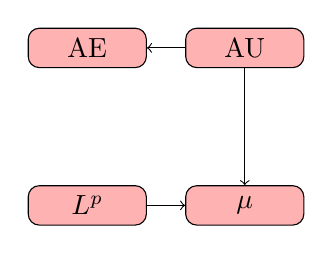
\begin{tikzpicture}[node distance=2cm]
% Reference: https://www.overleaf.com/learn/latex/LaTeX_Graphics_using_TikZ%3A_A_Tutorial_for_Beginners_(Part_3)%E2%80%94Creating_Flowcharts
\tikzstyle{roundrect} = [rectangle, rounded corners, minimum width=1.5cm, minimum height=.5cm,text centered, draw=black, fill=red!30]
\node (AE)[roundrect] {AE};
\node (Lp) [roundrect, below of=AE]{$L^p$};
\node (AU)[roundrect, right of=AE]{AU};
\node (mu)[roundrect, below of=AU]{$\mu$};
\draw [->] (AU) -- (AE);
\draw [->](AU) -- (mu);
\draw [->] (Lp) -- (mu);
\end{tikzpicture}
\caption{ \textit{Relationship between modes of convergence in a general measure space.} }
\label{fig:modes_of_convergence_general_measure_space}
\end{figure}


\begin{figure}[H]
\centering	
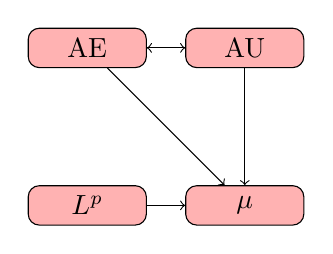
\begin{tikzpicture}[node distance=2cm]
% Reference: https://www.overleaf.com/learn/latex/LaTeX_Graphics_using_TikZ%3A_A_Tutorial_for_Beginners_(Part_3)%E2%80%94Creating_Flowcharts
\tikzstyle{roundrect} = [rectangle, rounded corners, minimum width=1.5cm, minimum height=.5cm,text centered, draw=black, fill=red!30]
\node (AE)[roundrect] {AE};
\node (Lp) [roundrect, below of=AE]{$L^p$};
\node (AU)[roundrect, right of=AE]{AU};
\node (mu)[roundrect, below of=AU]{$\mu$};
\draw [->] (AU) -- (AE);
\draw [->](AU) -- (mu);
\draw [->] (Lp) -- (mu);
\draw [->] (AE) -- (AU);
\draw [->] (AE) -- (mu);
\end{tikzpicture}
\caption{ \textit{Relationship between modes of convergence in a finite measure space.}}
\label{fig:modes_of_convergence_finite_measure_space}
\end{figure}


\begin{figure}[H]
\centering	
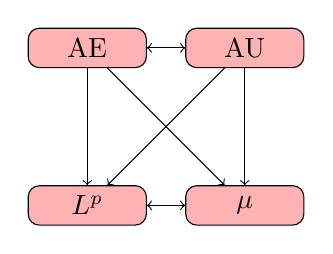
\begin{tikzpicture}[node distance=2cm]
% Reference: https://www.overleaf.com/learn/latex/LaTeX_Graphics_using_TikZ%3A_A_Tutorial_for_Beginners_(Part_3)%E2%80%94Creating_Flowcharts
\tikzstyle{roundrect} = [rectangle, rounded corners, minimum width=1.5cm, minimum height=.5cm,text centered, draw=black, fill=red!30]
\node (AE)[roundrect] {AE};
\node (Lp) [roundrect, below of=AE]{$L^p$};
\node (AU)[roundrect, right of=AE]{AU};
\node (mu)[roundrect, below of=AU]{$\mu$};
\draw [->] (AU) -- (AE);
\draw [->](AU) -- (mu);
\draw [->] (Lp) -- (mu);
\draw [->] (AE) -- (AU);
\draw [->] (AE) -- (mu);
\draw [->] (AE) -- (Lp);
\draw [->] (mu) -- (Lp);
\draw [->] (AU) -- (Lp);
\end{tikzpicture}
\caption{ \textit{Relationship between modes of convergence under a dominating function.} Here we assume the sequence $(f_n)$ is dominated by a function $g$ in $L^p$.  The measure space is general (not necessarily finite.)}
\label{fig:modes_of_convergence_under_dominating_function}
\end{figure}

We note:

\begin{itemize}
\item In a finite measure space, or when a dominating function exists, a.e. convergence becomes stronger than it is in general measure spaces. The additional two edges in moving from measure general spaces ( Fig.~\ref{fig:modes_of_convergence_general_measure_space}) to finite measure spaces  (Fig.~\ref{fig:modes_of_convergence_finite_measure_space}) are obtained from Egoroff's Theorem.   
\item When a dominating function exists, the same relations exist as in a finite measure space, along with three new ones.  In particular, the three other modes of convergence becomes stronger relative to $L^p$ convergence.  We note that in this context, \textit{a.e. convergence implies all three other modes of convergence}!
\end{itemize}


\subsection{Convergence on general measure spaces: Implications}

The implications in the section are powerful because they \textit{always} hold. In some special case, if one can prove that the antecedent holds, then the consequent automatically follows as well.

\subsubsection{Convergence in $L^p$ implies convergence in measure}
To relate $\convergenceInLp$ and $\convergenceInMu$, we can will utilize Chebyshev's Inequality. 

\begin{theorem}{\textbf{(Chebyshev's Inequality.)}}
Let $f : \Omega \to [0,\infty]$ be a Borel measurable function on $(\Omega, \F, \mu)$. 

If $0 < p < \infty$ and $0 < \epsilon < \infty$, then 
\[ \mu \set{\omega :  f(\omega) \geq \epsilon} \leq \frac{1}{\epsilon^p} \dint f^p \dmu \] 
\label{thm:chebyshevs_inequality}
\end{theorem}

\begin{proof}
Using monotonicity, we can obtain a lower bound the integral by the integral of a simple function. 

\begin{align*}
\dint_\Omega f^p \dmu \stackexplain{monotonicity}{\geq} \dint_{\set{\omega : f(\omega) > \epsilon}} f^p \dmu  \stackexplain{monotonicity}{\geq} 	\dint_{\set{\omega : f(\omega) > \epsilon}} \epsilon^p \dmu \stackexplain{int. simple func.}{=} \epsilon^p \mu\set{\omega : f(\omega) > \epsilon}
\end{align*}
\end{proof}

% TODO: Save the application of Chebyshev's Inequality to probability (as given by Ash) until we get to the actual probability section!
%\begin{remark}
%In the probability section, we will see that Chebyshev is often applied to $X$ being a rando	
%\end{remark}


\begin{remark}
The proof of Chebyshev's theorem highlights yet again the niceities of Lebesgue integration - we can integrate over any set we want (so long as the set is measurable), and those sets can be defined in terms of conditions in the range.  	
\end{remark}
 

Now we can show that convergence in $L^p$ is stronger than convergence in measure

\begin{theorem}
If $f_1, f_2, \hdots \in L^p \, (0 < p < \infty)$, then $f_n \convergenceInLp f \implies f_n \convergenceInMu f$. 
\label{thm:convergence_in_Lp_implies_convergence_in_measure}	
\end{theorem}

\begin{proof}
We have
%
\begin{align*}
& \forall \, \epsilon < 0, \exists N : \forall \, n \geq N, \\
& \mu \set{\omega : |f_n (\omega) - f(\omega)| \geq \epsilontilde}  \stackexplain{(1)}{\leq} \frac{1}{\epsilontilde^p} \dint |f_n -f|^p \dmu \stackexplain{(2)}{<} \epsilon 	
\end{align*}
%
where (1) is obtained by applying Chebyshev's Inequality to the non-negative function $|f_n -f|$, and (2) is obtained by the hypothesis of $L^p$ convergence. {\tiny (More precisely,  $L^p$ convergence can make $\dint |f_n -f|^p \dmu  < \epsilon_1$ for any desired $\epsilon_1 >0$ for sufficiently large $n$.  So we decompose we write $\epsilon = \frac{1}{\epsilontilde^p} \epsilon_1$.  Since $\epsilontilde^p$ is fixed, we can choose $\epsilon_1$ to get any desired $\epsilon.$)} 
\end{proof}


\subsubsection{Almost uniform convergence implies convergence almost everywhere and convergence in measure} 

Now we show that almost uniform convergence is stronger than convergence almost everywhere and convergence in measure.
\begin{theorem}
We have
\begin{alphabate}
\item $f_n \convergenceAU f \implies f_n \convergenceAE f$
\item $f_n \convergenceAU f \implies f_n \convergenceInMu f$		
\end{alphabate}
\label{thm:convergence_AU_implies_convergence_in_measure_and_convergence_AE}
\end{theorem}

\begin{proof}
\begin{alphabate}
\item TBD.
\item We take the definition of $\convergenceAU$ in quantified form \eqref{eqn:def_of_convergence_almost_uniformly_in_quantified_form} 
\begin{align*}
&\forall \, \epsilontilde >0, \exists \, A \in \F : \mu(A) < \epsilontilde \quad \text{and} \quad \forall \, \epsilon >0, \, \exists \, N : \forall \, n \geq N, \omega \in A^c \\
& |f_n(\omega) - f(\omega) | < \epsilon 
\end{align*}
and remove the explicit reference to the set $A$. In particular, for fixed $\epsilontilde, \epsilon>0$ and sufficiently large $n$, we have
\begin{align*} 
& \set{\omega : |f_n(\omega) - f(\omega) | \geq \epsilon  } \subset A \\
&\implies \mu\set{\omega : |f_n(\omega) - f(\omega) | \geq \epsilon  } \stackexplain{monotonicity of measure}{\leq} \mu(A) \stackexplain{hypoth}{<} \epsilontilde 
\end{align*}
So the original quantified statement becomes
\begin{align*}
&\forall \, \epsilontilde >0,  \epsilon >0, \exists \, N : \forall \, n \geq N \\
& \mu\set{\omega : |f_n(\omega) - f(\omega) | \geq \epsilon  } < \epsilontilde 
\end{align*}
which is the definition of convergence in measure. 
\end{alphabate}
\end{proof}

\subsection{Convergence on finite measure spaces: Implications}

As noted in Sec.~\ref{sec:overview_of_relations_between_modes_of_convergence}, finite measure spaces have two implications that doesn't exist for general measure spaces:  $f_n \convergenceAE f \implies f_n \convergenceAU f, f_n \convergenceInMu f$.  We obtain the former implication via Egoroff's Theorem, and then the latter follows immediately from Thm.~\ref{thm:convergence_AU_implies_convergence_in_measure_and_convergence_AE}.

\begin{theorem}\textbf{(Egoroff's Theorem.)} If $\mu$ is finite and $f_1, f_2, \hdots$ and $f$ are measurable complex-valued functions, then $f_n \convergenceAE f \implies f_n \convergenceAU f$.
\label{thm:egoroffs_theorem}
\end{theorem}

\begin{proof}
Without loss of generality, we assume $f_n \to f$ everywhere. {\tiny (If the implication holds for everywhere convergence, it must hold for a.e. convergence.  Suppose that $N$ is a set such that $\mu(N)=0$ and $f_n \to f$ outside $N$, and suppose that $A_\epsilon$ are the sets we have obtained for AU convergence from the weaker condition.  Then we simply form the sets $N \cup A_\epsilon$ in the definition of AU convergence, and we will automatically have $\mu(N \cup A_\epsilon) \stackexplain{subadditivity}{<} \mu(N) + \mu(A_\epsilon) < \epsilon)$ and uniform convergence will hold outside of $N \cup A_\epsilon$.)}

For $k,n \in \mathbb{N}$, define
\[E_n(k) := \explaintermbrace{Set of points whose outputs are at least $\frac{1}{k}$ away from the target somewhere in the tail starting at $n$}{\bigcup_{m=n}^\infty \bigg\{ x : |f_m(x) - f(x) | > \frac{1}{k} \bigg\}} \] 
Let us fix $k$, consider this a sequence of sets in $n$, and check the conditions for continuity from above:
\begin{itemize}
\item $E_n(k)$ decreases as $n$ increases? \greencheck. 
	\begin{itemize}
	\item Note: $\bigcap_{n=1}^\infty E_n(k) = \emptyset$ by hypothesis that $f_n \to f$ everywhere. 	
	\end{itemize}
\item $\mu(E_1(k)) < \infty$? \greencheck.  By hypothesis, $\mu$ is finite. 
\end{itemize}
Thus, by continuity from above, 
\[  \mu\big(E_n(k)\big) \to 0 \quad \text{as} \quad n \to \infty\]
As a result, given $\epsilon>0$ and $k \in \mathbb{N}$, we can choose $n_k$ so large that 
\[  \mu\big(E_{n_k}(k)\big) < \epsilon 2^{-k}\]
Now let $E := \cup_{k=1}^\infty E_{n_k}(k)$.  By subadditivity, we have
\[ \ \mu(E) \stackexplain{subadditivity}{\leq} \ds\sum_{k=1}^\infty \mu\big(E_n(k)\big) \stackexplain{see above}{<} \ds\sum_{k=1}^\infty \epsilon 2^{-k} \stackexplain{geometric series}{=} \epsilon  \]
Now we show that $f_n \to f$ uniformly on $E^c$.  Applying DeMorgan's law
\[E^c \stackexplain{def. E, DeMorgan}{=}  \bigcap_{k=1}^\infty E_{n_k}(k)^c  \stackexplain{def. $E_{n}$, DeMorgan}{=}\explaintermbrace{...for all $k$}{\bigcap_{k=1}^\infty \explaintermbrace{points within a $\frac{1}{k}$ distance of target in tail starting at $n_k$}{\bigcap_{m=n_k}^\infty \bigg\{ x: |f_m(x) - f(x)| < \frac{1}{k} \bigg\}}}  \]
Thus, $E^c$ describes precisely the points of uniform convergence. 
\end{proof}

\begin{remark}
The proof above utilizes a set theoretic definition of uniform convergence. See Remark~\ref{rk:set_theoretic_definition_of_uniform_convergence}.	
\end{remark}

\begin{remark}
Combining Egoroff's Theorem with Thm.~\ref{thm:convergence_AU_implies_convergence_in_measure_and_convergence_AE}, we obtain that if $\mu$ is finite, then 
\[ f_n \convergenceAE 0 \stackexplain{Egoroff's Theorem (Thm.~\ref{thm:egoroffs_theorem})}{\implies} f_n \convergenceAU 0 \stackexplain{Thm.~\ref{thm:convergence_AU_implies_convergence_in_measure_and_convergence_AE}}{\implies}  f_n \convergenceInMu 0  \]
This chain of implications explains the two new links that appear in Fig.~\ref{fig:modes_of_convergence_finite_measure_space} compared to Fig.~\ref{fig:modes_of_convergence_general_measure_space}.
\end{remark}

\subsection{Convergence under a dominating function: Implications}

\subsubsection{Convergence a.e. and convergence in $L^p$}

First we show that in general
\[ f_n \convergenceAE f \notimplies f_n \convergenceInLp f \]

Let $\Omega = [0, \infty)$ and $\mu$ be Lebesgue measure. Let $f_n = n \, \indicate{(0, \frac{1}{n}]}$.  Then $f_n \to 0$ a.e.  But 
\[ || f_n -0 ||_p^p = \dint_\Omega \bigg( n \, \indicate{(0, \frac{1}{n}]} \bigg)^p \dmu = n^p \mu((0,1/n]) = n^p (\frac{1}{n}) = n^{p-1} \not\to 0 \quad \text{as} \quad n \to \infty\]

However, if the sequence has a \textit{dominating function} (in $L^p$, i.e. its $p$th power is integrable), then the implication holds.

\begin{theorem}
\cite[Cor.~1.6.10]{ash2000probability}.  Let $f_1, f_2, \hdots, f, g$ be Borel measurable, and $|f_n| \leq g$ for all $n$, where $|g|^p$ is $\mu$-integrable $(p>0, \textnormal{fixed})$.  Then $f \in L^p$ and 
 \[ f_n \convergenceAE f \implies f_n \convergenceInLp f \]
\label{thm:ae_convergence_plus_dominating_function_implies_Lp_convergence}
\end{theorem}

\begin{proof}
First note that
\[ |f_n| \leq g \stackrel{1}{\implies} \lim_{n \to \infty } |f_n| \leq g \stackrel{2}{\implies} |f| \leq g\]
where (1) holds because limits preserve non-strict inequalities and (2) holds because limits and absolute values commute. 

From this, by raising both sides of the implication to the $p$-th power, we immediately obtain
\[ |f_n|^p \leq |g|^p, \quad |f|^p \leq |g|^p \]	

At this point, we know that $|f|^p$ is integrable (i.e. $f \in L^p$). 

Now we will apply the Dominated Convergence Theorem to show $L^p$ convergence.  First, we obtain a dominating function
\[ |f_n -f|^p \stackexplain{tr. inequal.}{\leq} (|f_n| + |f|)^p \stackexplain{from above}{\leq} (2 |g|)^p \stackexplain{hypoth.}{<} \infty\]

Then we have
%
\[ \dlim_{n \to \infty} \dint |f_n - f|^p \dmu \stackexplain{LDCT}{=} \dint \dlim_{n \to \infty}  |f_n - f|^p \dmu \stackexplain{1}{=}   0 \]
where (1) holds by the hypothesis of a.e. convergence (so $|f_n - f|^p =0$ a.e.) followed by the a.e. theorems (see Theorem \ref{thm:almost_everywhere} (a)). 
\end{proof}


We can use Theorem~\ref{thm:ae_convergence_plus_dominating_function_implies_Lp_convergence} to prove that finite-valued simple functions are dense in $L^p$.

\begin{theorem}\textnormal{(Finite valued simple functions are dense in $L^p$.)}
Let $f \in L^p, \; (0 < p < \infty)$. If $\epsilon >0$, there is a simple function $s \in L^p$ such that $||f-s||_p < \epsilon$; $s$ can be chosen to be finite-valued and to satisfy $|s| \leq |f|$.
\label{thm:finite_valued_simple_functions_are_dense_in_Lp}	
\end{theorem}

\begin{proof}
First note that Cor \ref{cor:measurable_function_is_limit_of_simple_functions_which_it_dominates} states that any measurable function  is the limit of a sequence of simple functions which it dominates.   In particular, we have
\[s_n \to f \quad \text{everywhere}, \quad\quad |s_n| < f \]
where $s_n$ is a sequence of finite-valued simple functions.

Since we have identified a.e. convergence and a dominating function with the correct integrability condition {\tiny (note that $|f|^p$ is $\mu$-integrable, since $f \in L^p$ by hypothesis.)}, we can apply Theorem~\ref{thm:ae_convergence_plus_dominating_function_implies_Lp_convergence} to obtain  $s_n \convergenceInLp f$.   

The conclusion immediately follows. {\tiny (For any $\epsilon>0$, we can choose an $n$ so that $||f-s_n||_p < \epsilon$.)}
 

\end{proof}


\subsection{Counterexamples}

The counterexamples below will prove the \textit{non}-existence of all 9 missing edges from the 12 possible edges in Figure~\ref{fig:modes_of_convergence_general_measure_space}.

\subsubsection{Counterexample 1: No other modes imply $L^p$ convergence in a finite (and therefore in a general) measure space}

This counterexample justifies the non-existence of the three crossed-out links in Fig.~\ref{fig:non_existing_relationships_between_modes_of_convergence_in_a_finite_space}. 

\begin{figure}[H]
\centering	
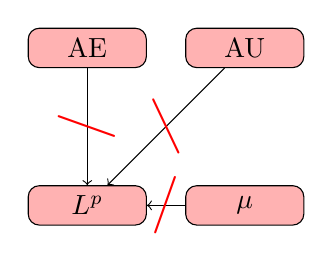
\begin{tikzpicture}[node distance=2cm]
% Reference: https://www.overleaf.com/learn/latex/LaTeX_Graphics_using_TikZ%3A_A_Tutorial_for_Beginners_(Part_3)%E2%80%94Creating_Flowcharts
\tikzstyle{roundrect} = [rectangle, rounded corners, minimum width=1.5cm, minimum height=.5cm,text centered, draw=black, fill=red!30]
\node (AE)[roundrect] {AE};
\node (Lp) [roundrect, below of=AE]{$L^p$};
\node (AU)[roundrect, right of=AE]{AU};
\node (mu)[roundrect, below of=AU]{$\mu$};
\draw [->] (AE) -- (Lp) node[pos=0.5,red,sloped] {\huge$/$} ;
\draw [->] (AU) -- (Lp) node[pos=0.5,red,sloped] {\huge$/$} ;
\draw [->] (mu) -- (Lp) node[pos=0.5,red,sloped] {\huge$/$} ;
\end{tikzpicture}
\caption{ \textit{Three non-existing relationships between modes of convergence in a finite (and therefore general) measure space.}  The non-existence of these links is justified by the counterexample in this section.}
\label{fig:non_existing_relationships_between_modes_of_convergence_in_a_finite_space}
\end{figure}


Let $\Omega=[0,1]$, $\mu$ be Lebesgue measure, and $\F$ be the Borel sets.  Define
\[f_n(x) =
\begin{cases}
e^n & \text{if} \quad 0 \leq x \leq \frac{1}{n} \\
0 & \text{otherwise}	
\end{cases}
 \]
 
\begin{figure}[H]
\centering
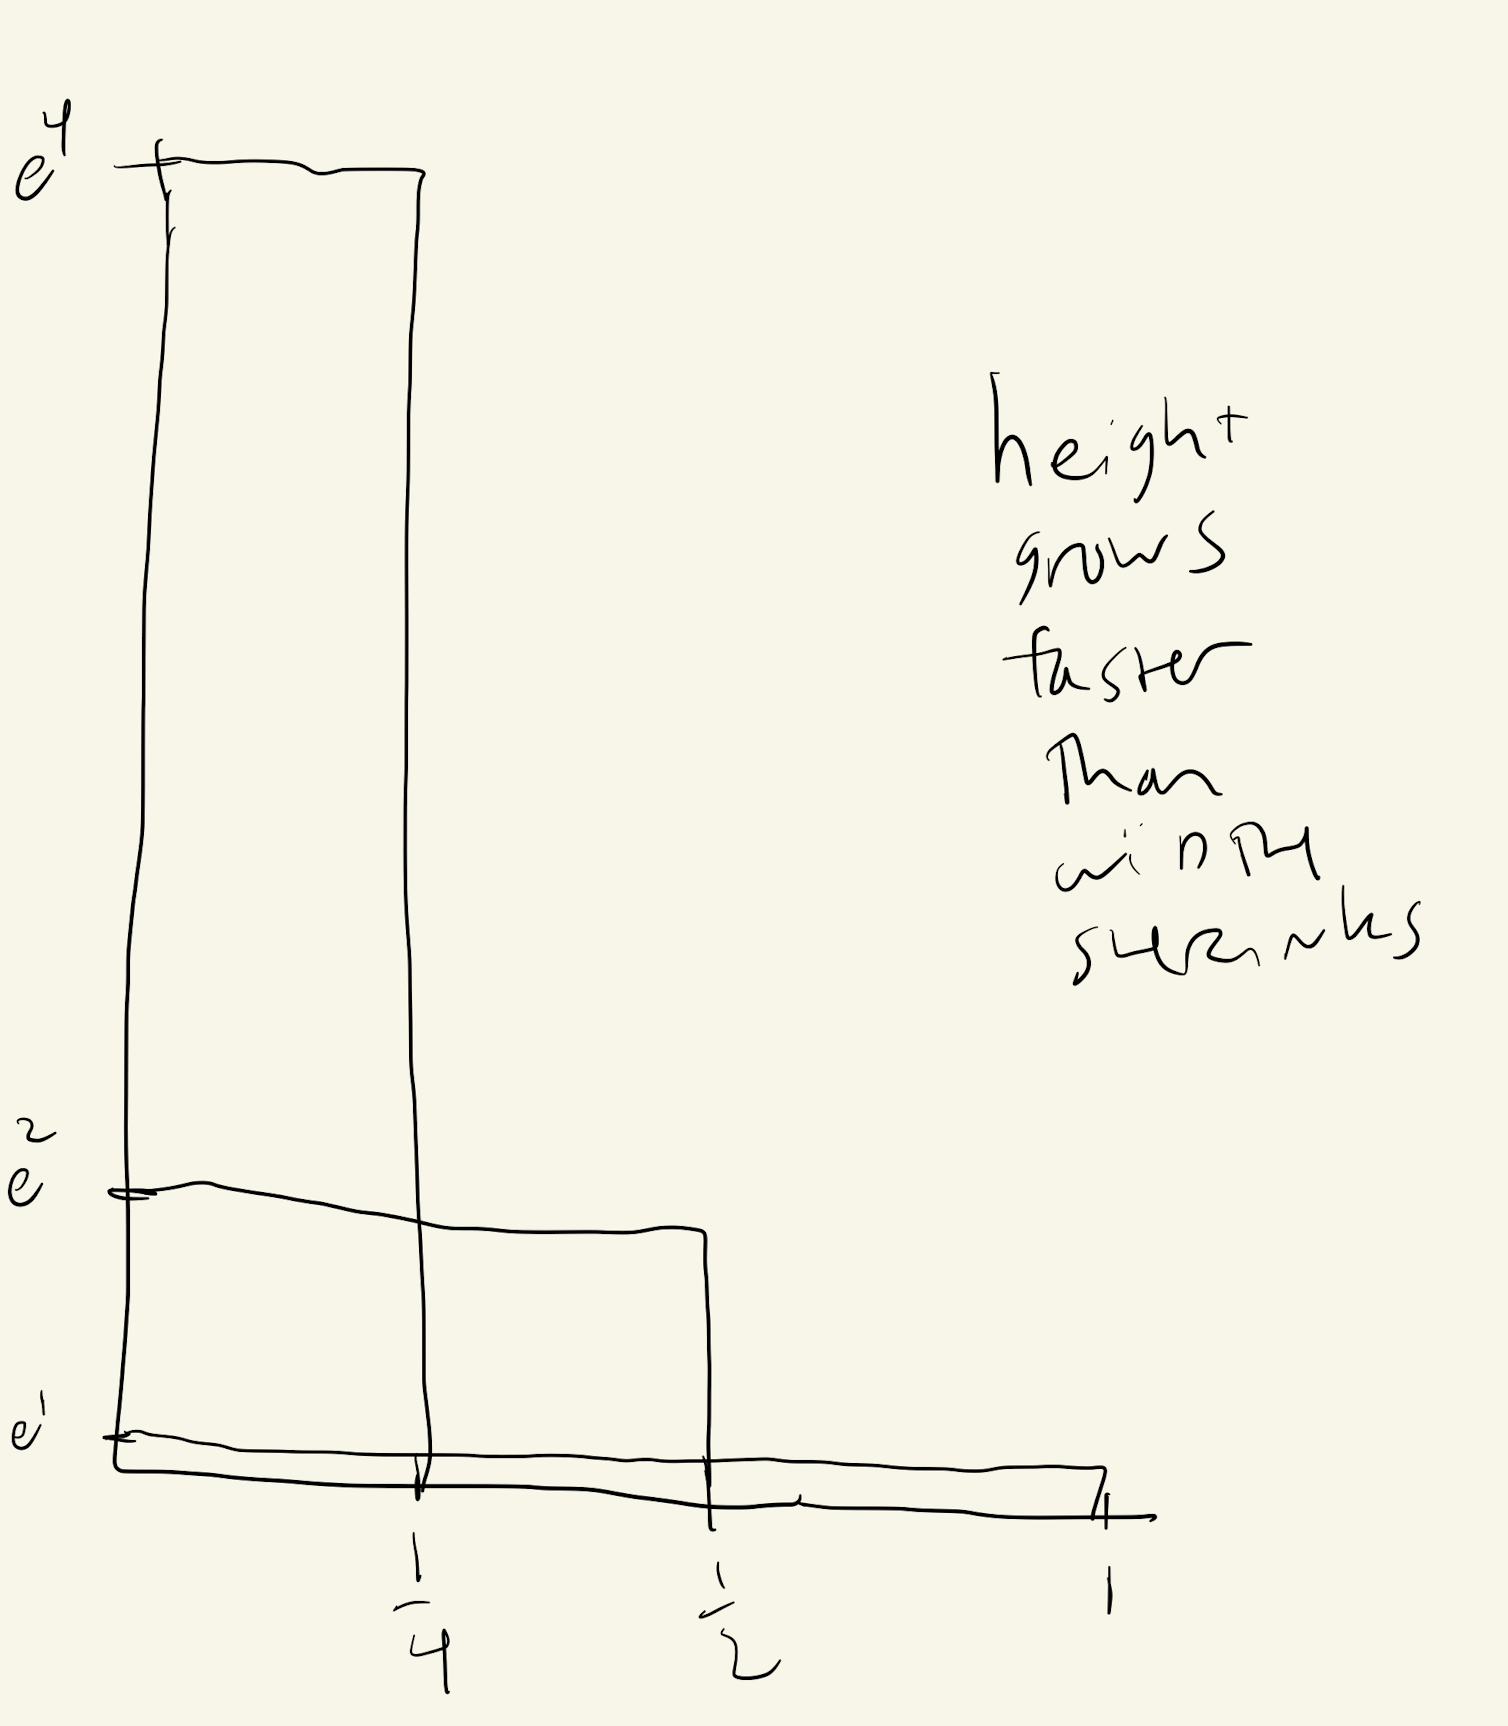
\includegraphics[width=.4\textwidth]{images/modes_of_convergence_counter_example_1}	
\caption{}
\label{fig:modes_of_convergence_counter_example_1}	
\end{figure}



Then clearly $f_n \convergenceAE 0$.  Moreover we have 
\[ f_n \convergenceAE 0 \stackexplain{Egoroff's Theorem (Thm.~\ref{thm:egoroffs_theorem})}{\implies} f_n \convergenceAU 0 \stackexplain{Thm.~\ref{thm:convergence_AU_implies_convergence_in_measure_and_convergence_AE}}{\implies}  f_n \convergenceInMu 0  \] 
{\tiny (Egoroff's Theorem  applies since the measure is finite.)} 

However, for $0 < p < \infty$, 
\begin{align}
||f_n||_p^p &= \int_0^1 \bigg|e^n \indicate{[0,\frac{1}{n}]} \bigg|^p \wrt{\mu} \nonumber \\
&= 	\int_0^1 e^{np}  \nonumber \indicate{[0,\frac{1}{n}]} \wrt{\mu} \nonumber  \\
&= e^{np} \mu \big[0,\frac{1}{n}\big] && \tinytext{int. simple func.} \nonumber  \\
&= e^{np} \frac{1}{n} \to \infty \nonumber %\label{eqn:modes_of_convergence_counterexample_one_height_grows_faster_than_width_shrinks}
\end{align}
And so $f_n \notConvergenceInLp 0$ for $p \in (0, \infty)$.

\begin{remark}{\remarktitle{Convergence in $L^\infty$.}}
Likewise, for $p=\infty$
\[ ||f_n||_\infty = e^n \to \infty \]
 so $f_n \notConvergenceInLp 0$ for $p=\infty$. 
\end{remark}

\subsubsection{Counterexample 2: Another counterexample showing that no other modes imply $L^p$ convergence in a general measure space}


We provide a second counterexample showing that no other modes imply $L^p$ convergence in a general measure space (see Fig.~\ref{fig:non_existing_relationships_between_modes_of_convergence_in_a_finite_space}). 

Let $\Omega=\R$, $\mu$ be Lebesgue measure, and $\F$ be the Borel sets.  Define
\[f_n(x) =
\begin{cases}
\frac{1}{n} & \text{if} \quad 0 \leq x \leq e^n \\
0 & \text{otherwise}	
\end{cases}
 \]
 
\begin{figure}[H]
\centering
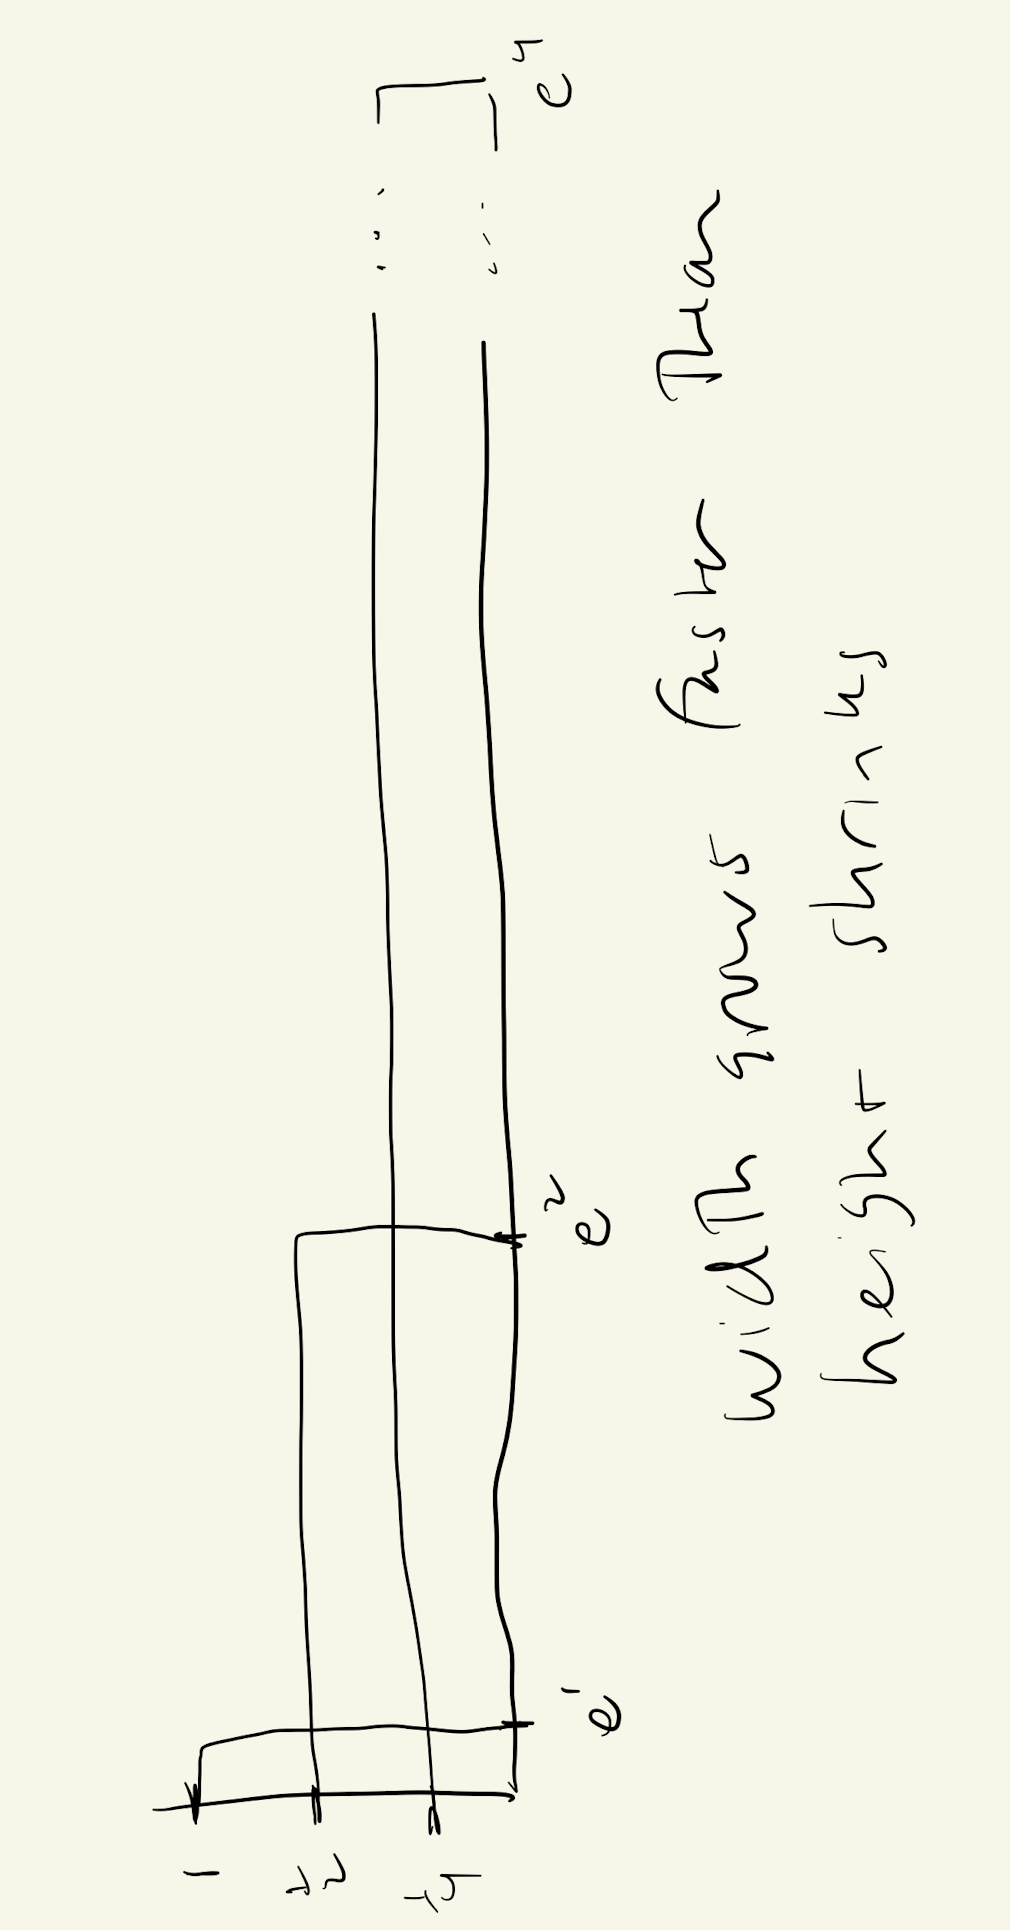
\includegraphics[width=.4\textwidth, angle=270]{images/modes_of_convergence_counter_example_2}	
\caption{}
\label{fig:modes_of_convergence_counter_example_2}	
\end{figure}

 Then $f_n \to 0$ uniformly on $\R$ {\tiny (Recall Def.~\ref{def:uniform_convergence}.)}  Thus, by Thm.~\ref{thm:convergence_AU_implies_convergence_in_measure_and_convergence_AE}, $f_n \convergenceAE 0, f_n \convergenceInMu 0$.
 
 However, for $0<p<\infty$,
 
 \begin{align*}
 ||f_n||_p^p &= \int \bigg| \frac{1}{n} \indicate{[0,e^n]} \bigg|^p \wrt{\mu} \\
 &= \big(\frac{1}{n}\big)^p \int \indicate{[0,e^n]}  \wrt{\mu} \\
 &= \big(\frac{1}{n}\big)^p \mu[0,e^n] \\
 &= \big(\frac{1}{n}\big)^p \; e^n \to \infty 
 \end{align*}



\begin{remark}{\remarktitle{Convergence in $L^\infty$.}}
Although $(f_n)$ does not converge in $L^p$ for $(0<p<\infty)$, it does converge in $L^\infty$. This is because uniform convergence a.e. implies convergence in $L^\infty$ ; see Remark~\ref{rk:L_infty_convergence_is_equivalent_to_uniform_cconvergence_ae}.
\end{remark}

\subsubsection{Counterexample 3: no other mode of convergence implies AU convergence in a general measure space}


Here we provide a counterexample showing that no other mode of convergence implies AU convergence in a general measure space.


\begin{figure}[H]
\centering	
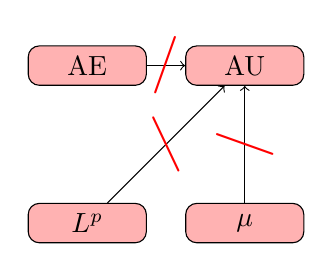
\begin{tikzpicture}[node distance=2cm]
% Reference: https://www.overleaf.com/learn/latex/LaTeX_Graphics_using_TikZ%3A_A_Tutorial_for_Beginners_(Part_3)%E2%80%94Creating_Flowcharts
\tikzstyle{roundrect} = [rectangle, rounded corners, minimum width=1.5cm, minimum height=.5cm,text centered, draw=black, fill=red!30]
\node (AE)[roundrect] {AE};
\node (Lp) [roundrect, below of=AE]{$L^p$};
\node (AU)[roundrect, right of=AE]{AU};
\node (mu)[roundrect, below of=AU]{$\mu$};
\draw [->] (Lp) -- (AU) node[pos=0.5,red,sloped] {\huge$/$} ;
\draw [->] (mu) -- (AU) node[pos=0.5,red,sloped] {\huge$/$} ;
\draw [->] (AE) -- (AU) node[pos=0.5,red,sloped] {\huge$/$} ;
\end{tikzpicture}
\caption{ \textit{Three more non-existing relationships between modes of convergence in a general measure space.}  The non-existence of these links is justified by the counterexample in this section.}
\label{fig:non_existing_relationships_between_modes_of_convergence_in_a_general_measure_space_nothing_implies_AU}
\end{figure}

Let $\Omega=[0,\infty)$, $\mu$ be Lebesgue measure, and $\F$ be the Borel sets.  Define
\[f_n(x) =
\begin{cases}
1 & \text{if} \quad n \leq x \leq n+ \frac{1}{n} \\
0 & \text{otherwise}	
\end{cases}
 \]
 
\begin{figure}[H]
\centering
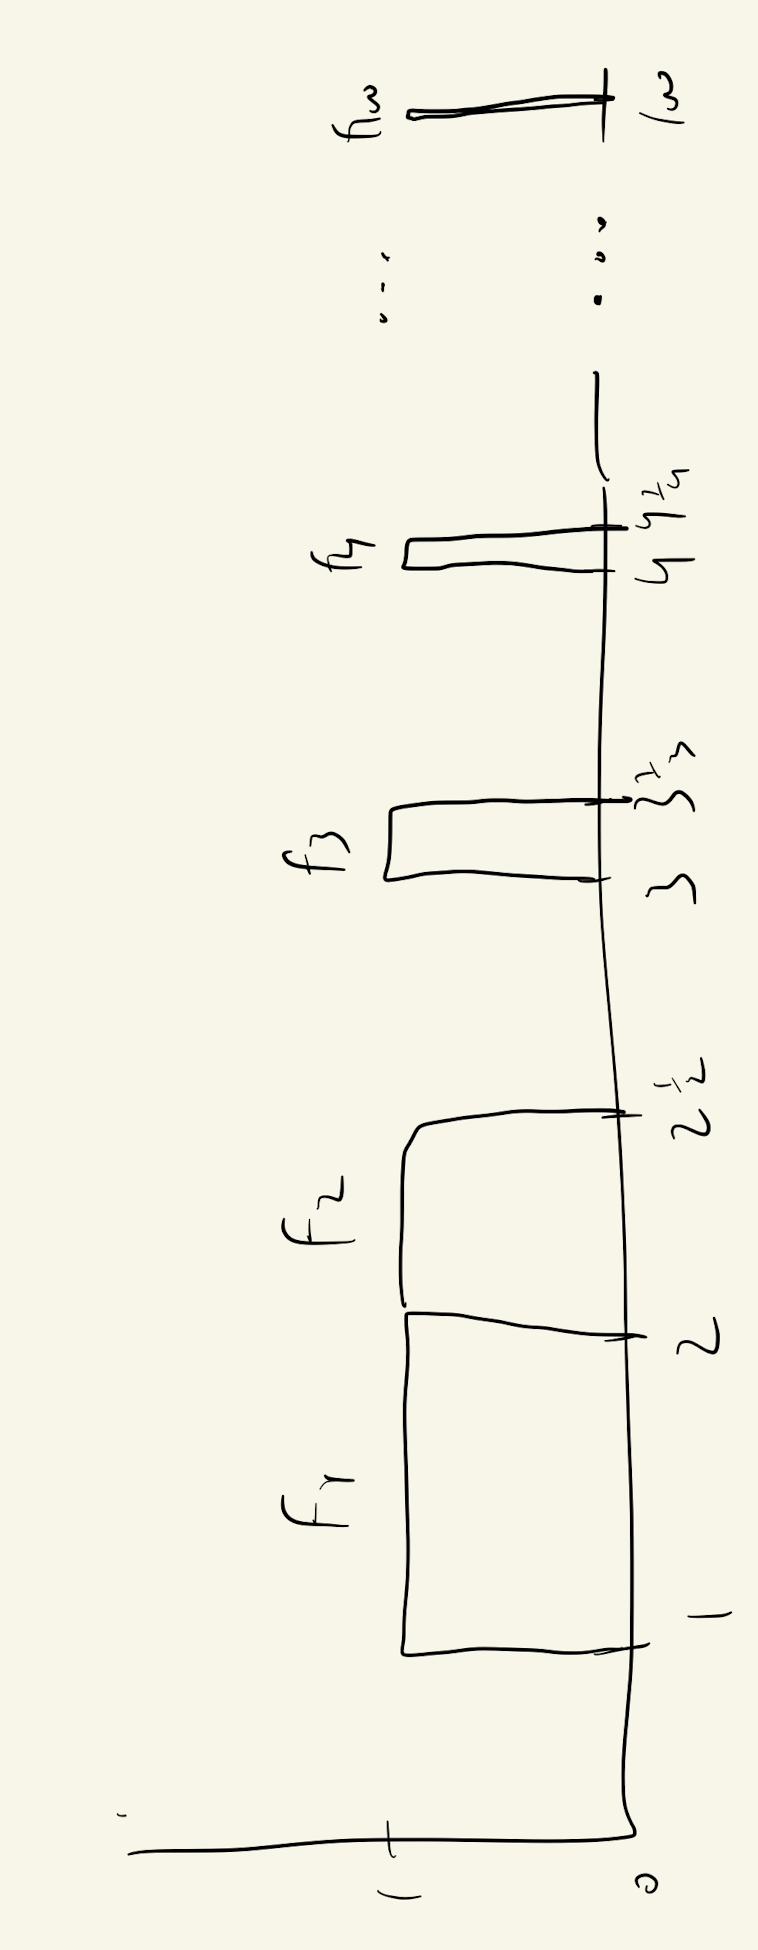
\includegraphics[width=.25\textwidth, angle=270]{images/modes_of_convergence_counter_example_3}	
\caption{}
\label{fig:modes_of_convergence_counter_example_3}	
\end{figure}

We first show that convergence holds AE, in $\mu$, and in $L^p$.
\begin{itemize}
\item $f_n \convergenceAE 0$? \greencheck  Clearly $f_n \to 0$ pointwise.	
\item $f_n \convergenceInLp 0$? \greencheck  
\[ ||f_n||_p^p = \int \bigg| \indicate{[n, n + \frac{1}{n}} \bigg|^{\cancel{p}} \wrt{\mu} = \mu\big[n , n+\frac{1}{n}\big] = \frac{1}{n} \to 0 \quad \text{as} \quad n \to \infty\]
\item $f_n \convergenceInMu 0$? \greencheck This is implied by convergence in $L^p$ (Thm.~\ref{thm:convergence_in_Lp_implies_convergence_in_measure}).  Alternatively, we could check directly. For all $\epsilon >0$,
\[ \mu \big\{ x : |f_n(x)| \geq \epsilon \big\} = \frac{1}{n} \to 0 \quad \text{as} \quad n \to \infty \]  
\end{itemize}

But $(f_n)$ does not converge AU (see \cite[pp.99]{ash2000probability}.
 

\subsubsection{Counterexample 4: Convergence in $L^p$ or in $\mu$ does not imply convergence  AE or AU}


Here we provide a counterexample showing that convergence in $L^p$ (and therefore measure) does not imply convergence AE (and therefore AU).


\begin{figure}[H]
\centering	
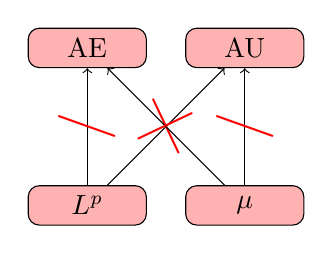
\begin{tikzpicture}[node distance=2cm]
% Reference: https://www.overleaf.com/learn/latex/LaTeX_Graphics_using_TikZ%3A_A_Tutorial_for_Beginners_(Part_3)%E2%80%94Creating_Flowcharts
\tikzstyle{roundrect} = [rectangle, rounded corners, minimum width=1.5cm, minimum height=.5cm,text centered, draw=black, fill=red!30]
\node (AE)[roundrect] {AE};
\node (Lp) [roundrect, below of=AE]{$L^p$};
\node (AU)[roundrect, right of=AE]{AU};
\node (mu)[roundrect, below of=AU]{$\mu$};
\draw [->] (Lp) -- (AU) node[pos=0.5,red,sloped] {\huge$/$} ;
\draw [->] (Lp) -- (AE) node[pos=0.5,red,sloped] {\huge$/$} ;
\draw [->] (mu) -- (AU) node[pos=0.5,red,sloped] {\huge$/$} ;
\draw [->] (mu) -- (AE) node[pos=0.5,red,sloped] {\huge$/$} ;
\end{tikzpicture}
\caption{ \textit{Four more non-existing relationships between modes of convergence in a finite (and therefore general) measure space.}  The non-existence of these links is justified by the counterexample in this section. (Note that the absence of link from $L^p$ to $AU$ was already justified in Fig.~\ref{fig:non_existing_relationships_between_modes_of_convergence_in_a_general_measure_space_nothing_implies_AU}.)}
\label{fig:non_existing_relationships_between_modes_of_convergence_Lp_and_measure_do_not_imply_AE_or_AU}
\end{figure}

Let $\Omega=(0,1]$, $\mu$ be Lebesgue measure, and $\F$ be the Borel sets.  Define
\[f_{nm}(x) =
\begin{cases}
1 & \text{if} \quad \frac{m-1}{n}  < x \leq \frac{m}{n}, \quad\quad m=1,\hdots,n, \quad n=1,2,\hdots \\
0 & \text{elsewhere}	
\end{cases}
 \]
 
\begin{figure}[H]
\centering
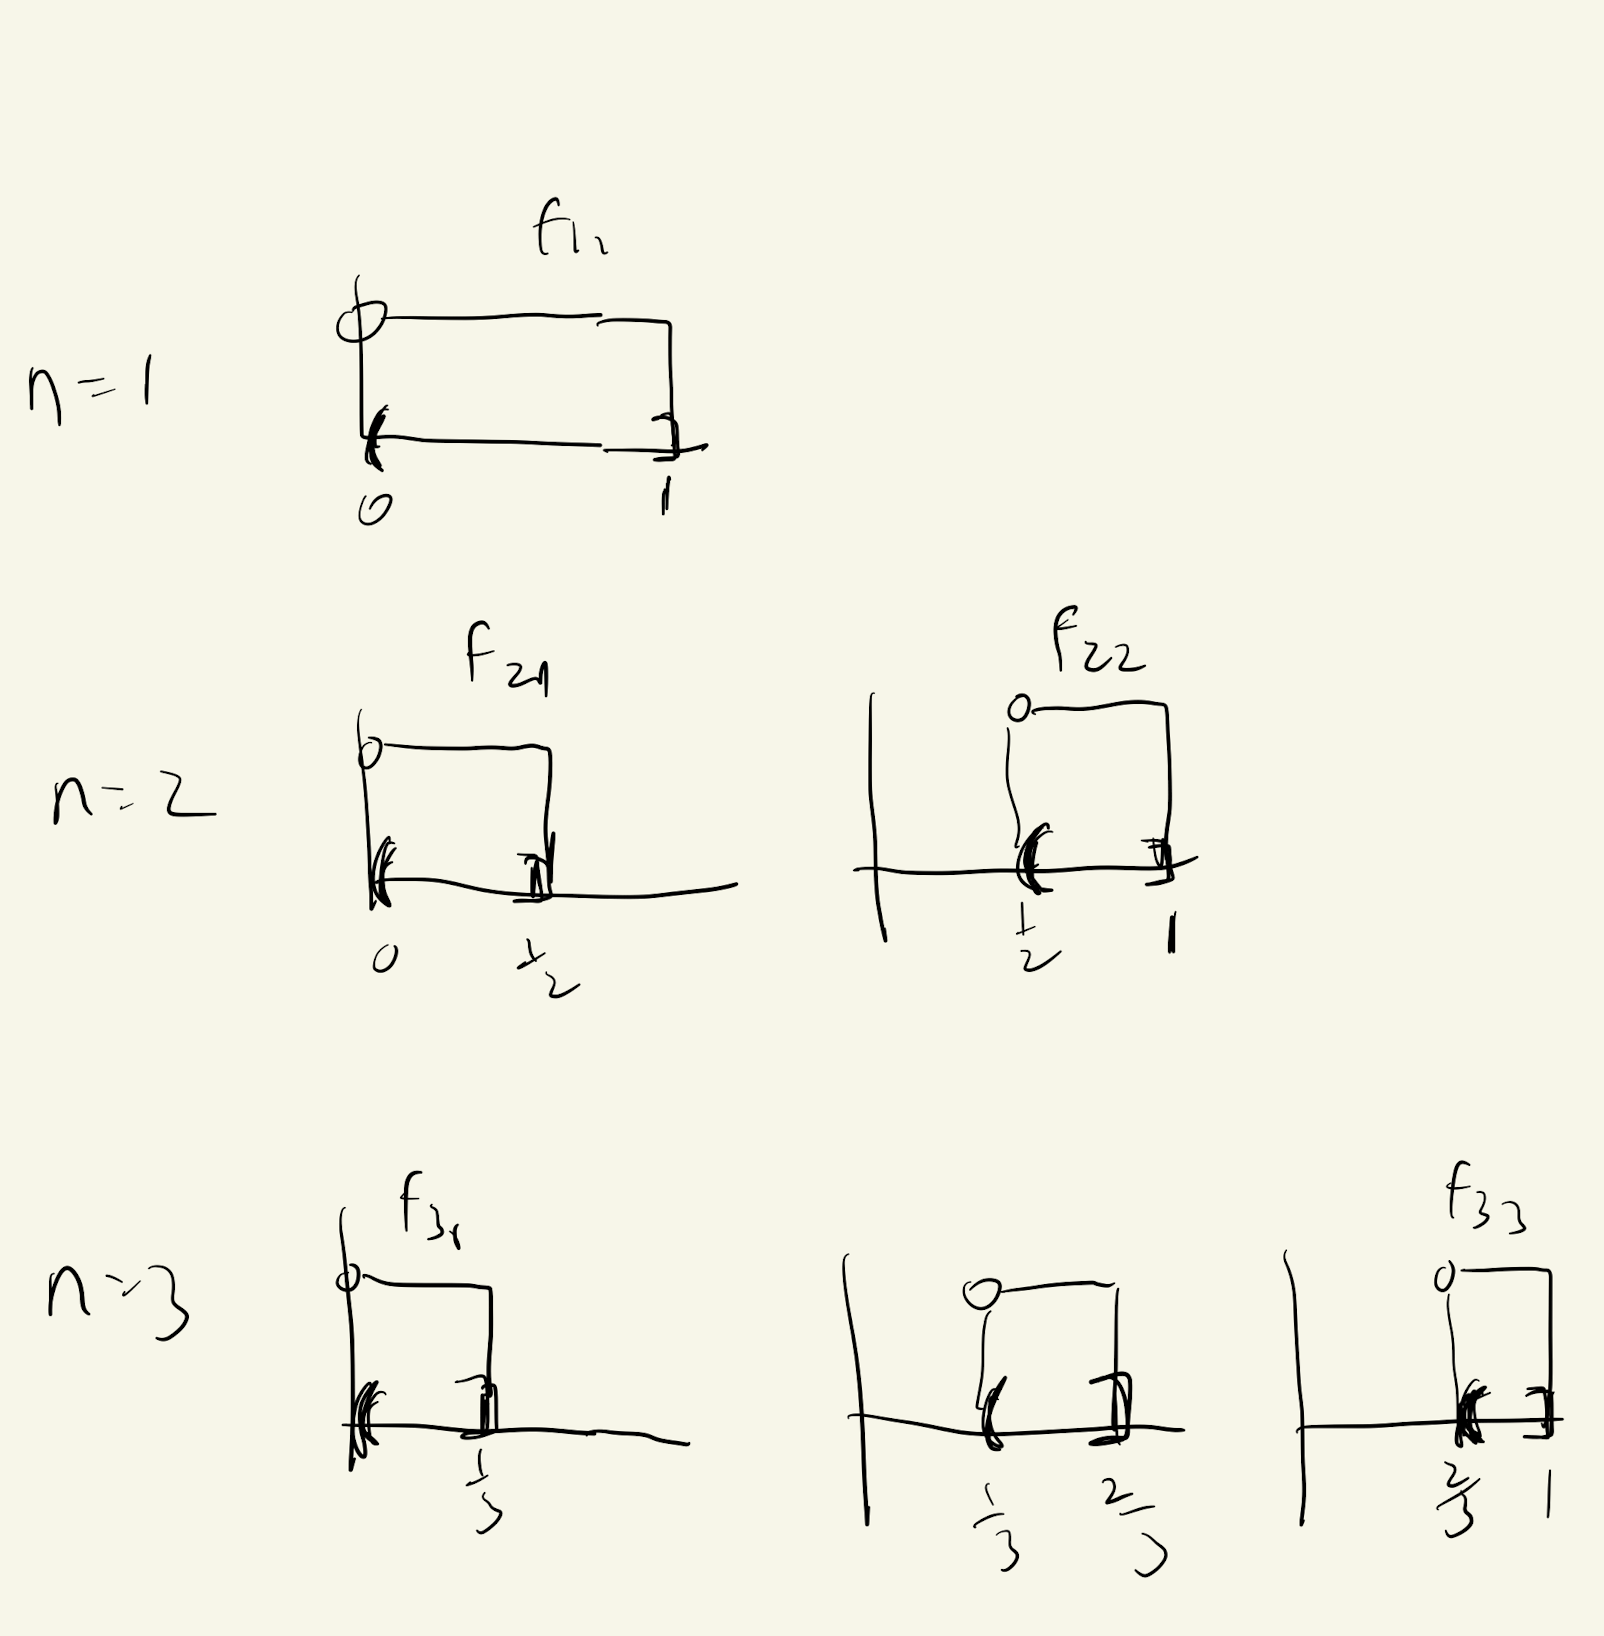
\includegraphics[width=.4\textwidth]{images/modes_of_convergence_counter_example_4}	
\caption{}
\label{fig:modes_of_convergence_counter_example_4}	
\end{figure}

We construct a sequence of  functions $f_{nm}$ by ordering the functions first by $n$ and then by $m$.

Now $f_{nm} \not\to 0$ a.e. {\tiny (since for any $x \in (0,1], f_{nm}(x)$ has infinitely many 0's and 1's).}. Thus, $f_{nm} \notConvergenceAU 0$, by Thm.~\ref{thm:convergence_AU_implies_convergence_in_measure_and_convergence_AE}.
 
 However, $f_{nm}\convergenceInLp 0$ for $0<p<\infty$, since
  
 \begin{align*}
 ||f_{nm}||_p^p &= \int \bigg| f_{nm} \bigg|^p \wrt{\mu} \\
 &= \int \indicate{[\frac{m-1}{n} < x \leq \frac{m}{n}]}  \wrt{\mu} \\
 &= \mu \bigg[\frac{m-1}{n}, \frac{m}{n}\bigg] \\
 &= \frac{1}{n} \to 0. 
 \end{align*}

Hence, $f_{nm} \convergenceInMu 0$ by Theorem~\ref{thm:convergence_in_Lp_implies_convergence_in_measure}. 


\begin{remark}
Although $(f_n)$ does not converge in $L^p$ for $(0<p<\infty)$, it does converge in $L^\infty$. This is because uniform convergence a.e. implies convergence in $L^\infty$ ; see Remark~\ref{rk:L_infty_convergence_is_equivalent_to_uniform_cconvergence_ae}.
\end{remark}


\section{$\S$ 2.6 Product measures and Fubini's theorem}

\subsection{Product $\sigma$-fields}


Throughout this section, let $(X,\M)$ and $(Y,\N)$ be measurable spaces.\footnote{For this section, we follow \url{https://www.math.ucdavis.edu/~hunter/measure_theory/measure_notes_ch5.pdf}.  First, the notation for sections seems nicer - and more commonly used - than Ash's.  Second, the presentation is more modular (e.g., the proposition that sections of a measurable set are measurable in buried in Ash's general product measure proof.)}

\begin{definition}
A \textbf{measurable rectangle} is a subset $A \times B$ of $X \times Y$ where $A \in \M$ and $B \in \N$ are measurable subsets of $X$ and $Y$, respectively.\footnote{See Def.~\ref{def:cartesian_product} for the definition of the Cartesian product.}
\end{definition}

\begin{remark}{\remarktitle{Measurable rectangles need not have intervals for ``sides".}}
The ``sides" of a measurable rectangle $A \times B$ are not required to be intervals.  For instance, if $\R$ is equipped with the Borel $\sigma$-field, then $\Q \times \Q$ is a measurable rectangle in $\R \times \R$. 	
\end{remark}

\begin{figure}[H]
\centering
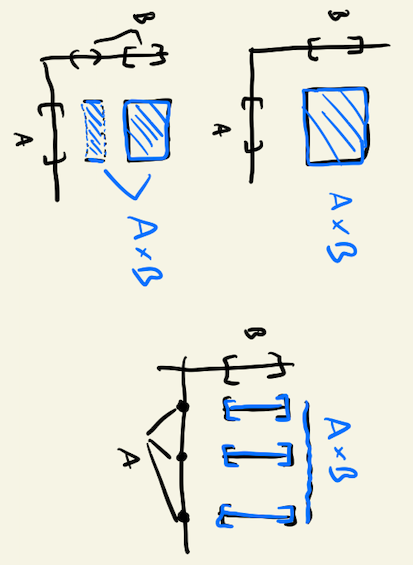
\includegraphics[width=.4\textwidth, angle=90]{images/measurable_rectangles}	
\caption{Three examples of measurable rectangles.}
\label{fig:three_examples_of_measurable_rectangles}
\end{figure}


\begin{definition}
The \textbf{product $\sigma$-field} $\M \otimes \N$ is the $\sigma$-field on $X \times Y$ generated by the collection of all measurable rectangles.
\[ \M \otimes \N := \sigma(\{ A \times B : A \in \M, \, B \in \N \})\]
\end{definition}

\begin{definition}{\textbf{Sections of sets.}}
Suppose that $E \subset X \times Y$.  For any $x \in X$ and $y \in Y$, we define the \textit{x-section} $E_x \subset Y$ and \textit{y-section} $E^y \subset X$ by:
\[ E_x := \set{y \in Y : (x,y) \in E}, \quad E^y := \set{x \in X : (x,y) \in E} \]
\end{definition}

\begin{figure}[H]
\centering
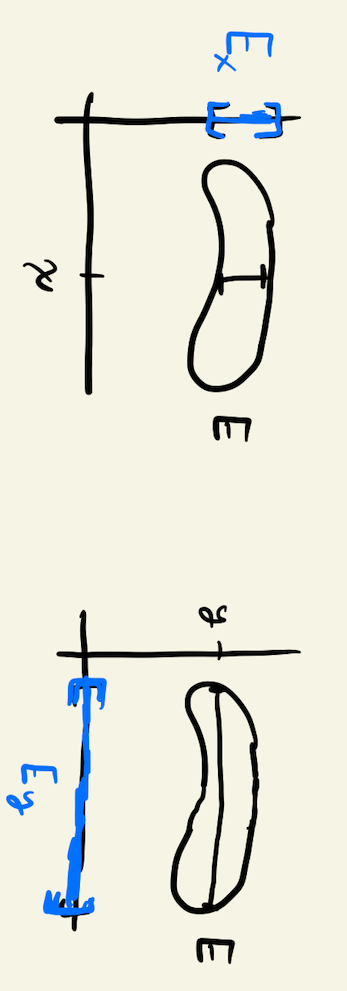
\includegraphics[width=.2\textwidth, angle=90]{images/sections}	
\caption{The \textit{x-section} and \textit{y-section} of a set $E$. }
\end{figure}

\begin{example}{\remarktitle{Sections of rectangles.}}
Given a rectangle $A \times B \subset X \times Y$, the sections are given by  
\begin{align}
(A \times B)_x = 
\begin{cases}
B,& x \in A \\
\emptyset, & x \not\in A	
\end{cases} \quad \quad \quad 
(A \times B)^y = 
\begin{cases}
A,& y \in B \\
\emptyset, & y \not\in B 	
\end{cases}
\label{eqn:sections_of_rectangles}
\end{align}
{\tiny For intuition, see Fig.~\ref{fig:three_examples_of_measurable_rectangles}.}
\label{ex:sections_of_rectangles}
\end{example}


\begin{proposition}{\remarktitle{All sections of a measurable set are measurable.}} If $(X,\M)$ and $(Y,\N)$ are measurable spaces, and $E \in \M \otimes \N$, then $E_x \in \M$ for every $x \in X$ and $E^y \in \N$ for every $y \in Y$. 
\label{prop:sections_of_a_measurable_set_are_measurable}
\end{proposition}

\begin{proof}
We apply the ``Good sets strategy" (Sec.~\ref{sec:good_sets_strategy}).   Let
\[  \G := \{ E \subset X \times Y : E_x \in \N \text{ for all} \; x \in X \quad \text{and} \quad E^y \in \M \text{ for all} \; y \in Y \}. \]
We have
\begin{itemize}
\item $\G$ contains all measurable rectangles, since the sections of $A \times B$ are given by \eqref{eqn:sections_of_rectangles}.
\item $\G$ is a $\sigma$-field, since, for example, if $E,E_i \subset X \times Y$ and $x \in X$, then 
\begin{align}
\explaintermbrace{section of complement}{(E^c)_x} = \explaintermbrace{complement of section}{(E_x)^c}, \quad \quad \quad \explaintermbrace{section of union}{\bigg(
\bigcup_{i=1}^\infty E_i \bigg)_x} = \explaintermbrace{union of sections}{\bigcup_{i=1}^\infty (E_i)_x}.  	
\label{eqn:sections_commute_with_complements_and_unions}
\end{align}

\begin{figure}[H]
\centering
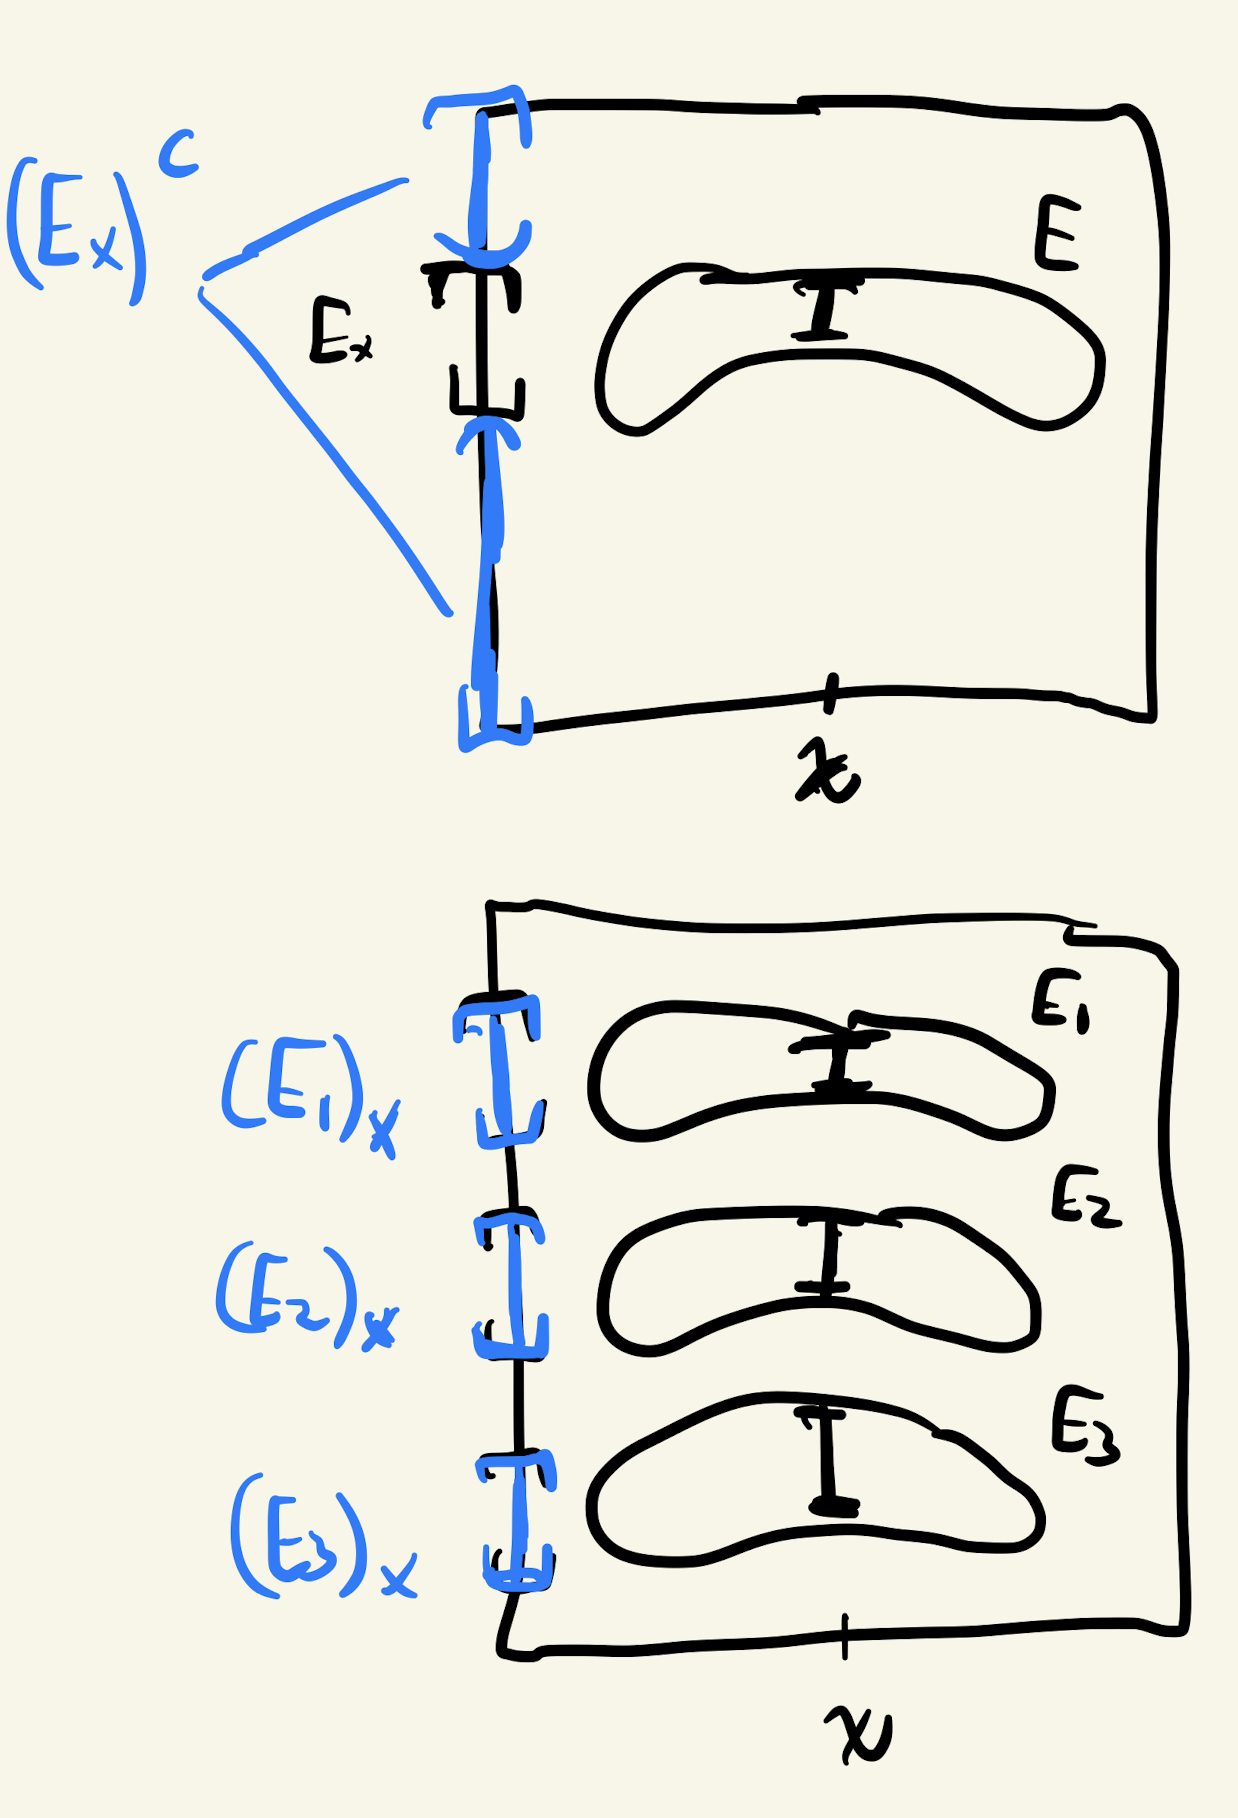
\includegraphics[width=.33\textwidth]{images/section_complement_and_union}	
\caption{\textit{Complement and union of a section}. Note the complement of the section is the section of the complement, and the union of sections is the section of the union.}
\end{figure}

\end{itemize}
\end{proof}

\subsection{Product measure} \label{sec:product_measure}

Here we follow \cite[pp.64]{folland1999real}.  Let $(X,\M, \mu)$ and $(Y,\N, \nu)$ be measure spaces. We have already discussed the product $\sigma$-algebra $\M \otimes \N$ on $X \times Y$.  Now we construct a measure on $\M \otimes \N$ that is, in an obvious sense, the product of $\mu$ and $\nu$. 

\subsubsection{Preliminaries}

\begin{remark}{\remarktitle{Measurable rectangles are an elementary family.}}

The set of measurable rectangles is an elementary family (Def.~\ref{def:elementary_family}).  First, we see that rectangles are closed under intersection.

\begin{figure}[H]
\centering 
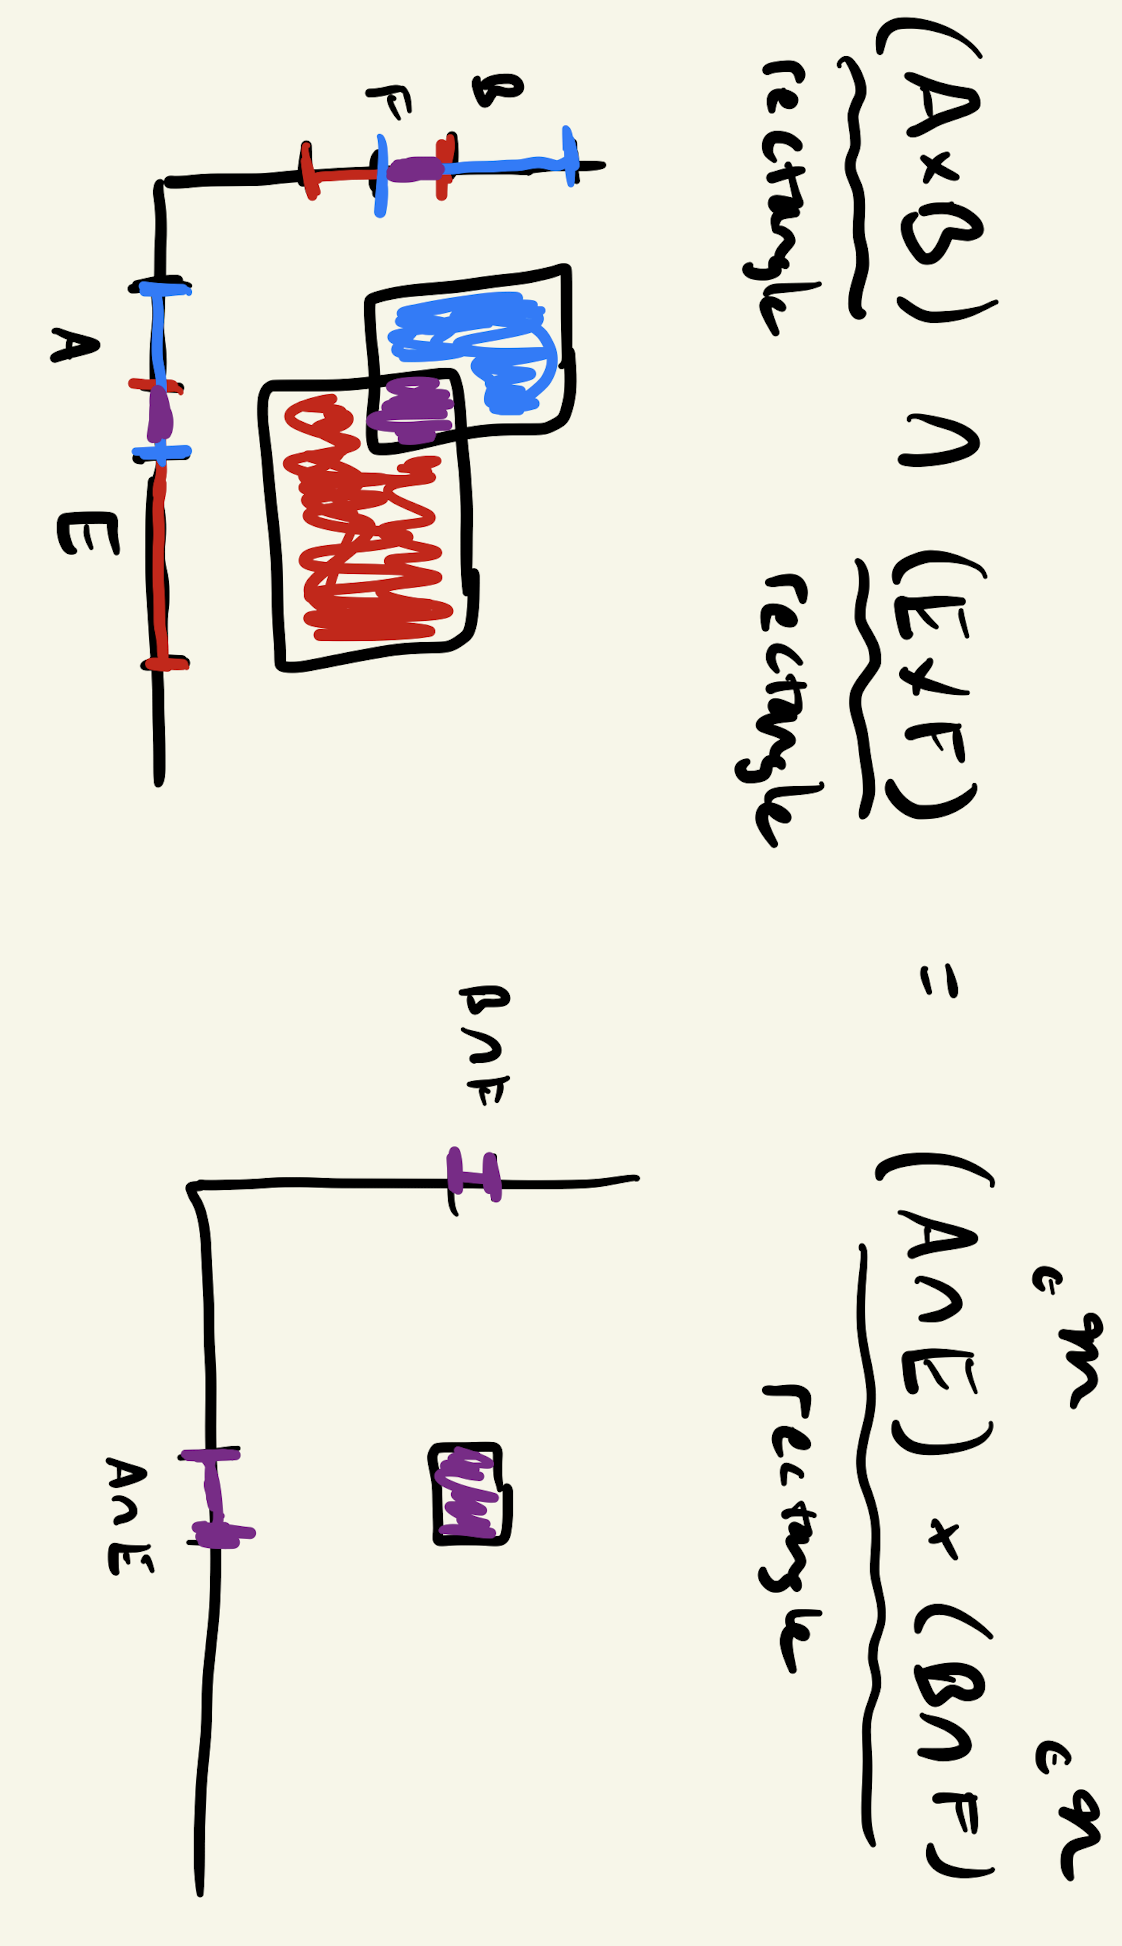
\includegraphics[width=.4\textwidth, angle=90]{images/rectangles_are_closed_under_intersection}	
\end{figure}

{\tiny We can formally prove this as follows:

\begin{align*}
(A \times B) \cap (E \times F)	&= \set{ (x,y) : x \in A, y \in B} \cap \set{ (x,y) : x \in E, y \in F} \\
&= \set{ (x,y) : x \in A \cap E , y \in B \cap F} \\
= (A \cap E) \times (B \cap F)
\end{align*}
}

Similarly, the complement of a rectangle is a disjoint union of rectangles:

\begin{figure}[H]
\centering 
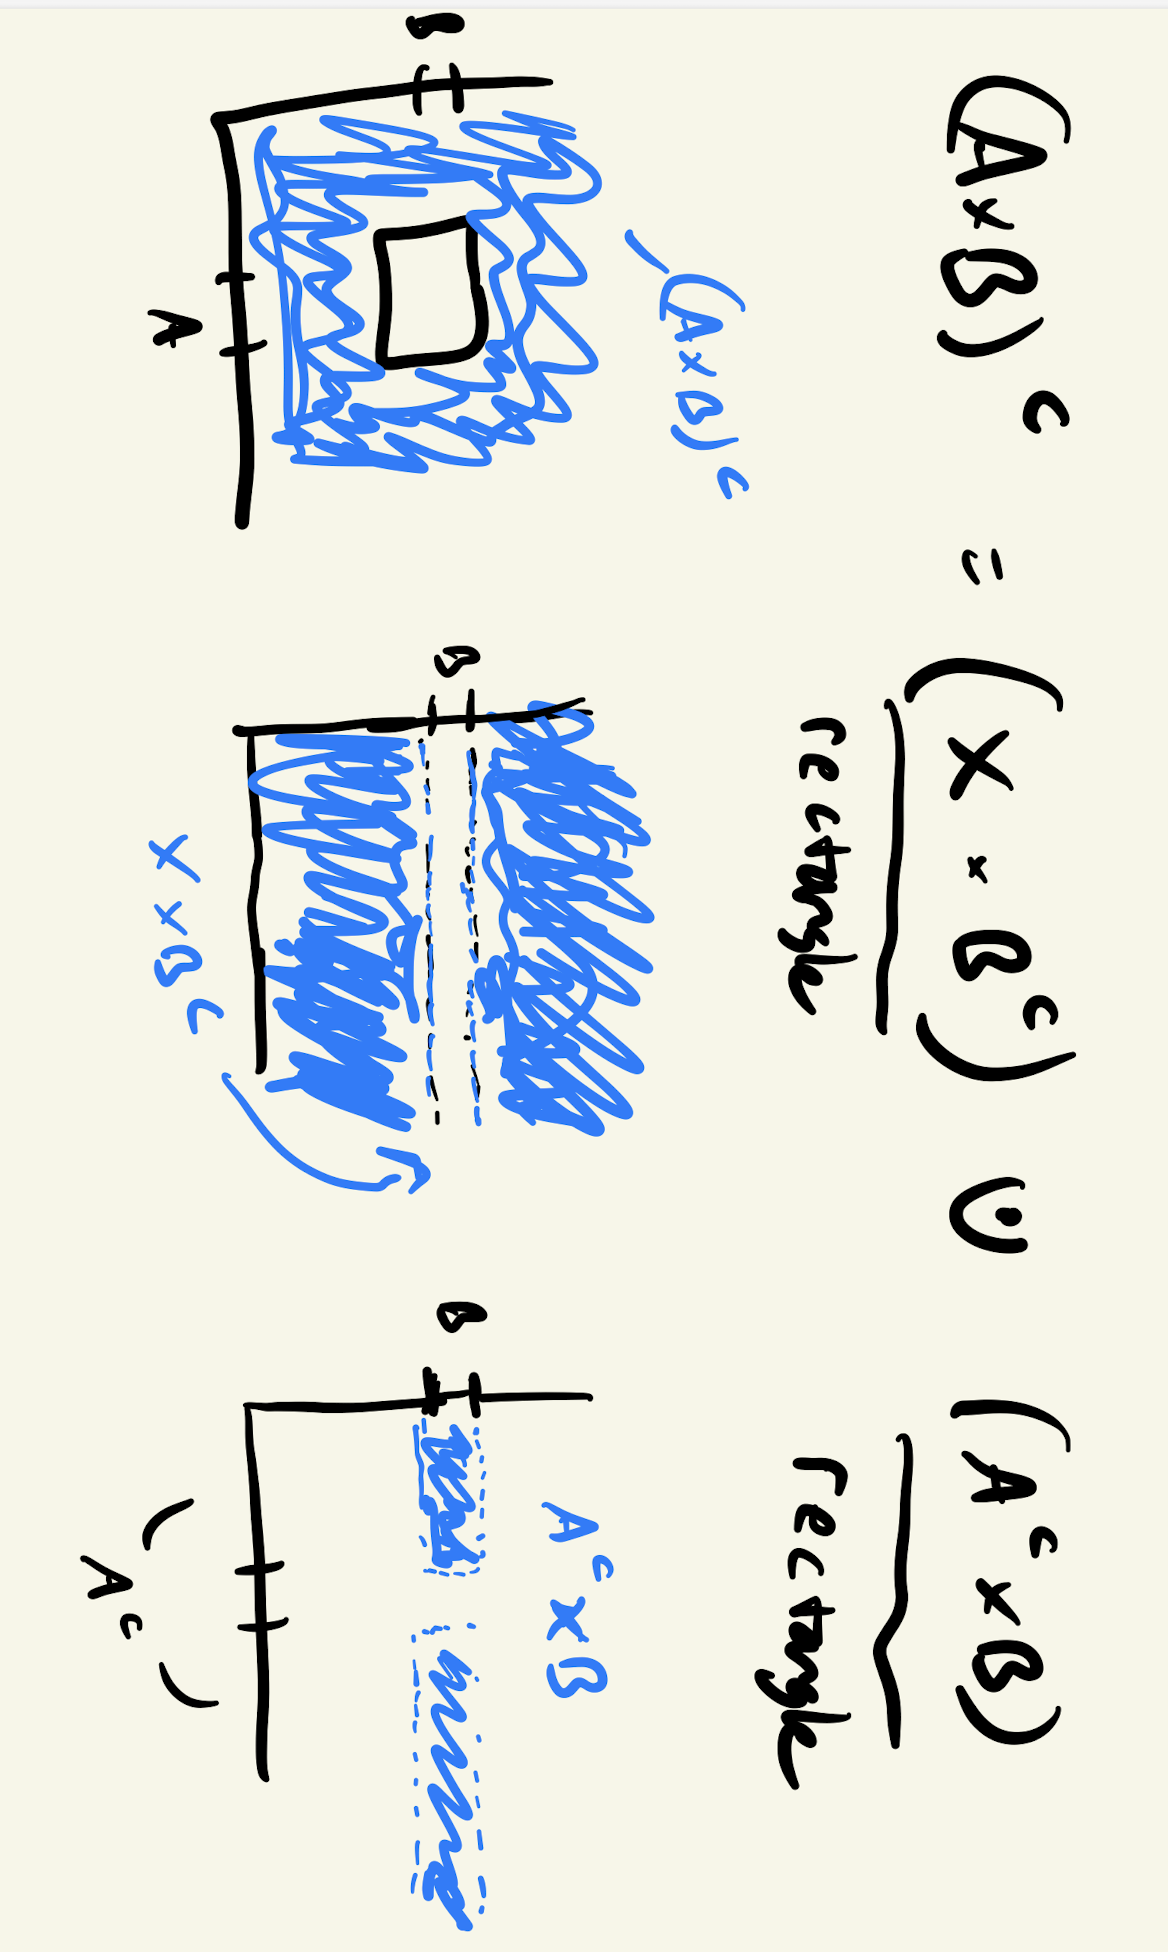
\includegraphics[width=.4\textwidth, angle=90]{images/complement_of_a_rectangle_is_a_disjoint_union_of_rectangles}	
\end{figure}
\label{rk:measurable_rectangles_are_an_elementary_family}
\end{remark}

\begin{remark}{\remarktitle{The collection of finite disjoint unions of rectangles is a field.}}
	
This follows immediately from Remark~\ref{rk:measurable_rectangles_are_an_elementary_family} and Proposition~\ref{prop:from_elementary_families_to_fields}.

Note that this collection now includes sets that aren't rectangles 

\begin{figure}[H]
\centering 
\includegraphics[width=.4\textwidth, angle=90]{images/disjoint_union_of_rectangles_neednt_be_a_rectangle}	
\end{figure}
\label{rk:the_collection_of_finite_disjoint__unions_of_rectangles_is_a_field}
\end{remark}


\subsubsection{Construction of the product measure} \label{sec:construction_of_the_product_measure}

Let $C \in F_0$ be a finite disjoint union of rectangles $A_1 \times B_1, A_2 \times B_2, \hdots A_n \times B_n$.  {\tiny  (By Remark Rk.~\ref{rk:the_collection_of_finite_disjoint__unions_of_rectangles_is_a_field},  $F_0$ is a field. ) }

Define the set function 
\[ \pi_0 (C) := \ds\sum_{i=1}^n \mu(A_i) \nu(B_i) \]
Then $\pi_0$ is well-defined, and a premeasure on $\F_0$ (see \cite[pp.64]{folland1999real} for a brief argument). 

By the \Caratheodory~Extension Theorem, $\pi_0$ extends to a measure $\pi$ on $\F:=\sigma(\F_0)$.  Moroever, it can be given constructively (see \eqref{eqn:explicit_construction_of_measure_extended_from_premeasure}) as follows:
\begin{subequations}
\begin{align}
\pi(E) &= \inf \bigg\{ \ds\sum_{i=1}^\infty \pi_0 (C_j) : C_j \in \F_0,  E \subset \cup_{j=1}^\infty C_j \bigg\} && \tinytext{} \label{eqn:direct_def_of_product_measure} \\	
& \quad \quad \quad \quad  \quad \quad \quad  \text{ where }  \pi_0 (C_j) = \ds\sum_{i=1}^{n_j} \mu(A_{ji}) \nu(B_{ji})  \nonumber \\
&=\inf \bigg\{ \ds\sum_{k=1}^\infty \mu(A_k) \nu(B_k) : A_k \in \M, B_k \in \N, \;  E \subset \cup_{k=1}^\infty (A_k \times B_k) \bigg \} && \tinytext{by reindexing} \label{eqn:computational_def_of_product_measure}	
\end{align}
\end{subequations}

{\tiny Eq.~\eqref{eqn:direct_def_of_product_measure} is the \textit{direct} definition of product measure, given directly by the explicit construction of a measure extended from a pre-measure.   Eq.~\ref{eqn:computational_def_of_product_measure} can be considered the \textit{computational} definition of product measure; the reindexing simplifies the infimum to be directly over rectangles rather than over disjoint unions of them. For an application of \eqref{eqn:computational_def_of_product_measure}, see Ex.~\ref{ex:lebesgue_counting_measure_on_the_unit_square_diagonal}.) }

The measure $\pi$ is called the product of $\mu$ and $\nu$, and is written $\pi = \mu \times \nu$.  Note that by \Caratheodory~Extension theorem {\tiny (or direct manipulation of the infimum)}, $\pi|_{\F_0} = \pi_0$.  Note also that (obviously) $\sigma(\F_0) = \M \otimes \N$, the product sigma-field.  

\begin{remark}
When $(X,\M, \mu)$ and $(Y,\N, \nu)$ are $\sigma$-finite measure spaces, the product measure is uniquely determined \cite[pp.64]{folland1999real}
\end{remark}
 

\subsection{Extended product measure theorem}

Below we get an alternate view on the product measure as integrated measures of sections (see Cor.~\ref{cor:classical_product_measure_theorem}).   But \cite{ash2000probability} actually works with a more general construction, which we might call an ``extended product measure".  This extended product measure seems like it will be useful for conditional probabilities. 

\begin{theorem}\textbf{(Extended product measure theorem.)} \cite[Thm.~2.6.2]{ash2000probability}
Consider the measure spaces $(X, \M, \mu), (Y, \N, \nu(x, \cdot))$, where 
\begin{itemize}
\item $\nu(x,A)$ is Borel measurable in $x$ for each fixed $A \in A$
\item $\nu(x, \cdot)$ are uniformly $\sigma$-finite \tiny{ (i.e., $Y= \bigcupdot_{n=1}^\infty B_n$, where $\nu(x,B) \leq k_n$ for all $x \in X$)}.	
\end{itemize}
Then $\exists!$ a measure $\lambda$ on $\F := \M \otimes \N$ such that 
\[\lambda(A \times B) = \int_A \nu(x,B) \mu(dx) \quad \quad \forall A \in \M, B \in \N \]
Namely
\begin{align}
\lambda(E) = \int_X \nu(x,E_x) \mu(dx), \quad \quad \forall E \in \F
\label{eqn:measure_of_set_in_product_space}
\end{align}
\label{thm:extended_product_measure_theorem}
\end{theorem}

\begin{remark}
Theorem~\ref{thm:extended_product_measure_theorem} says that the measure of a set $E \in \F$ is obtained as follows: for each $x \in X$, compute the measure of $E_x$, the section of $E$ at $x$, by $\nu(\explaintermbrace{parameter}{x}, \explaintermbrace{set to be measured}{E_x})$.  Then integrate this over all $x$, weighted by the measure on $X$. 
\begin{figure}[H]
\centering
\includegraphics[width=.4\textwidth]{images/product_measure_theorem}	
\end{figure}

\end{remark}


\begin{proof}
First assume that the $\nu(x, \cdot)$ are finite.
\begin{enumerate}
\item[(1.)] If $E \in \F$, then $\nu(x, E_x)$ is Borel measurable in $x \in X$. (For a proof, see item (2) of the proof in \cite{ash2000probability}).\redfootnote{TODO: Add my proof.}
\item[(2.)] Define 
\[ \lambda(E) = \int_A \nu(x,E_x) \mu(dx), \quad \quad \forall E \in F\] 
The integral exists by (1.) {\tiny(since the integral of a non-negative Borel measurable function always exists)}.   Then 
	\begin{alphabate}
	\item \textit{$\lambda$ is a measure on $\F$.}  To see this note that 
	\begin{align*}
	\lambda (\cupdot_{n=1}^\infty E_n) &\stackexplain{def}{=} \int_X \nu\bigg(x, (\cupdot_{n=1}^\infty E_n)_x \bigg) \mu(dx) \\
	& \stackexplain{(+)}{=} \int_X \sum_{n=1}^\infty \nu\bigg(x, (E_n)_x \bigg) \mu(dx) \\
	&\stackexplain{Ash Cor 1.6.4}{=} \sum_{n=1}^\infty \int_X  \nu\bigg(x, (E_n)_x \bigg) \mu(dx) \\
	&\stackexplain{def}{=} \sum_{n=1}^\infty \lambda(E_n) 
	\end{align*}
	To justify (+), we have 
	\begin{align*}
	(\cupdot_{n=1}^\infty E_n)_x &= \cupdot_{n=1}^\infty (E_n)_x && \tinytext{sections commute with unions, \eqref{eqn:sections_commute_with_complements_and_unions}} \\
	\implies \nu\bigg(x,(\cupdot_{n=1}^\infty E_n)_x\bigg) &= \nu\bigg(x,\cupdot_{n=1}^\infty (E_n)_x\bigg)  && \tinytext{substitution} \\
	&= \sum_{n=1}^\infty \nu \bigg(x, (E_n)_x\bigg) && \tinytext{countable additivity. each $(E_n)_x$ is measurable by   Prop.~\ref{prop:sections_of_a_measurable_set_are_measurable}, hence so is the union}
	\end{align*}
	\item Moreoever,
	\[\lambda(A \times B) = \int_A \nu(x,B) \mu(dx) \quad \quad \forall A \in \M, B \in \N \]
	To see this, note that
	\begin{align*}
	\lambda(A \times B) &\stackexplain{def.}{=} \int_X \nu \bigg(x, (A \times B)_x \bigg) \mu(dx)\\
	& \stackexplain{(*)}{=} \int_X \nu (x, B_x) \indicate{x \in A} \, \mu(dx) \\
	& = \int_A \nu (x, B_x) \,  \mu(dx)
	\end{align*}
	where (*) holds since by sections of rectangles (Example~\ref{ex:sections_of_rectangles}), we have $\nu \big(x, (A \times B)_x \big) = \nu (x, B_x) \indicate{x \in A}$.
	\end{alphabate}
\end{enumerate}

For an extension to the uniformly $\sigma$-finite case, and to show uniqueness, see \cite{ash2000probability}.
\end{proof}

\begin{question}
I'm not sure that $\lambda$ in Thm~\ref{thm:extended_product_measure_theorem} should be called a product measure.  Other references use product measure solely to refer to the more restricted object given below in Cor.~\ref{cor:classical_product_measure_theorem}.  So how shall we refer to $\lambda$ in Thm~\ref{thm:extended_product_measure_theorem} by name?  As a joint measure?  As an extended product measure?
\end{question}


\begin{corollary}\textbf{(Classical product measure theorem.)}
Let $(X, \M, \mu)$ and $(Y, \N, \nu)$ be $\sigma$-finite measure spaces.  Then the set function given by 
\[ \pi(E) := \int \nu(E_x) \mu(dx) = \int \mu(E^y) \nu(dy) \]
is the unique measure on $\M \otimes \N$ such that 
\[ \pi(A \times B) = \mu(A) \nu(B) \]
for all $A \in \M, B \in \N$.  Moreover, $\pi$ is $\sigma$-finite on $\M \otimes \N$, and is a probability measure if $\mu$ and $\nu$ are.  The measure $\pi$ is called the product of $\mu$ and $\nu$, and is written $\pi = \mu \times \nu$.
\label{cor:classical_product_measure_theorem}
\end{corollary}

\begin{proof}
In Theorem~\ref{thm:extended_product_measure_theorem}, take $\nu(x, \cdot) = \nu$ for all $x \in X$.  The second formula for $\pi$ is obtained by interchanging $\mu$ and $\nu$.	
\end{proof}

\subsection{Classical Fubini-Tonelli theorem}

In this section, we follow \cite{folland1999real} in restricting our consideration to classical product measures (as defined in Cor.~\ref{cor:classical_product_measure_theorem}).  For more general statements that work with extended product measures (as defined in Theorem.~\ref{thm:extended_product_measure_theorem}), see \cite[pp.105]{ash2000probability}. 

\begin{definition}\textbf{(Sections of functions)} If $f$ is a function on $X \times Y$, we define the \textbf{x-section} $f_x$ and \textbf{y-section} $f^y$ by
\[ f_x(y) = f^y(x) = f(x,y)\] 	
\end{definition}

So the section is obtained by fixing one variable and letting the other vary. 

\begin{example}
\[ (\indicate{E})_x =  \indicate{{E_x}} \quad \text{and} \quad (\indicate{E})_y =  \indicate{{E_y}}  \]

{\tiny We prove the left hand side only (as the right side follows immediately by interchanging variables). By definition of sections of functions, we have
\[\bigg(\indicate{E}\bigg)_x = \bigg(\indicate{ \set{(x,y) : (x,y) \in E}}\bigg)_x \stackexplain{def. sections of functions}{=} \indicate{\set{y: (x,y) \in E}}\] 
By definition of sections of sets, we have
\[ \indicate{{E_x}} = \indicate{\set{y: (x,y) \in E}} \]
since by definition, $E_x := \set{y \in Y : (x,y) \in E}$. 
}
\end{example}


The classical Fubini-Tonelli Theorem tells us when integrating against product measure is the same as iterated integration in either order. 

\begin{theorem}\textbf{Classical Fubini-Tonelli Theorem.}   Suppose that $(X,\M,\mu)$ and $(Y, \N, \nu)$ are $\sigma$-finite measure spaces.  
\begin{alphabate}
\item (Tonelli.) If $f$ is a non-negative measurable function on $X \times Y$ then
\[ g(x) = \int f_x \wrt{\nu}, \quad \quad h(y) = \int f^y \wrt{\mu} \]
are non-negative measurable functions on $X$ and $Y$, respectively, and 
\begin{align}
\int f \wrt{(\mu \times \nu)} = \int \int f(x,y) \wrt{\nu(y)}   \wrt{\mu(x)}  = \int \int f(x,y) \wrt{\mu(x)}  \wrt{\nu(y)}   
\label{eqn:classical_fubini_tonelli_equation}
\end{align}
\item (Fubini.) If $f \in L^1(\mu \times \nu)$ then 
	\begin{enumerate}
		\item[i)] $f_x \in L^1(\nu)$ for a.e. $x \in X$, \quad $f^y \in L^1(\mu)$ for a.e. $y \in Y$
		\item[ii)] $g(x) = \int f_x \wrt{\nu} \in L^1(\mu),  \quad h(y) = \int f^y \wrt{\mu} \in L^1(\nu)$
	\end{enumerate}
and \eqref{eqn:classical_fubini_tonelli_equation} holds.
\end{alphabate}	
\label{thm:classical_fubini_tonelli}
\end{theorem}

\begin{proof}
Our proof of Fubini-Tonelli mimics the construction of the integral.   

We begin with Tonelli's, which covers the first three steps.
\begin{enumerate}
\item \textit{Step 1: $f$ is an indicator function}.   Here, Tonelli's theorem reduces to the classical product measure theorem {\tiny  [If $f=\indicate{E}$, then \eqref{eqn:classical_fubini_tonelli_equation} becomes $\pi(E) := \int \nu(E_x) \mu(dx) = \int \mu(E^y) \nu(dy) $, which holds by   Cor.~\ref{cor:classical_product_measure_theorem}.]}   % Note that when integrating $f(x,y)$ against one variable, the function becomes a section.  So when integrating $f(x,y)$ against a measure on $y$, it becomes $f_x(y)$.]}  
\item \textit{Step 2: $f$ is a non-negative simple function.}  Here, Tonelli's theorem follows from step 1 and linearity. {\tiny (Recall linearity always applies for non-negative simple functions; see Remark~\ref{rk:integrals_are_linear_over_non_negative_Borel_measurable_function}.)}  
\item \textit{Step 3: $f$ is a general non-negative measurable function}.  We can find a sequence of simple functions $\set{f_n} \uparrow f$ by Prop.~\ref{prop:there_is_a_sequence_of_simple_fucntions_that_increases_to_any_non_negative_borel_measurable_function}.   We now show two things:
	\begin{itemize}
	\item The inner integrands $g, h$ are measurable. To see this, define corresponding sequences $\set{g_n}, \set{h_n}$ via 
	\[ g_n(x) = \int (f_n)_x \wrt{\nu}, \quad \quad h_n(y) = \int (f_n)^y \wrt{\mu} \]
	Since $f_n \uparrow f$, by Monotone Convergence Theorem, $g_n \uparrow g, h_n \uparrow h$. Thus, $g, h$ are measurable. 
	\item Tonelli's theorem holds.  To see this, we apply Monotone Convergence Theorem again {\tiny (this time on $g_n \uparrow g, h_n \uparrow h$)}, and we obtain 
	\begin{align*}
	\int g \dmu & \stackexplain{MCT
	}{=} \lim_n \int g_n \dmu  \\
	&\stackexplain{def $g_n$
	}{=}\lim_n \int \bigg( \int (f_n)_x \wrt{\nu} \bigg) \dmu \\
	& \stackexplain{def sec. of functions}{=} \lim_n \int \bigg( \int f_n(x,y) \wrt{\nu(y)} \bigg) \dmu(x) \\
	& \stackexplain{Step 2}{=} \lim_n \int f_n \wrt{(\mu \times \nu)} \\
	& \stackexplain{MCT}{=} \int f \wrt{(\mu \times \nu)}
	\end{align*}
	which is the first equality of \eqref{eqn:classical_fubini_tonelli_equation}.  The second equality is obtained by applying the same logic to $h$. 
	\end{itemize}
\end{enumerate}
Now we do Fubini's part of the theorem.  We start by verifying the conditions (i),(ii), and then show that \eqref{eqn:classical_fubini_tonelli_equation} holds (which parallels ``Step 4" in the construction of the integral).

\begin{itemize}
\item[i)] 
\begin{align*} 
f \in L^1(\mu \times \nu) &\iff \int f \wrt{(\mu \times \nu)} < \infty  && \tinytext{by definition} \\
& \iff \int |f| \wrt{(\mu \times \nu)} < \infty \\
& \iff \int \int |f| \wrt{\mu} \wrt{\nu} = \int \int |f| \wrt{\nu} \wrt{\mu} < \infty && \tinytext{Tonelli} \\
& \iff \int \int f \wrt{\mu} \wrt{\nu} = \int \int f \wrt{\nu} \wrt{\mu} < \infty \\
& \implies \explaintermbrace{$:=h(y)$}{\int f^y \wrt{\mu(x)}} < \infty \; \text{ a.e. } y , \quad \explaintermbrace{$:=g(x)$}{\int f_x \wrt{\nu(y)}} < \infty  \text{ a.e. } x && \tinytext{Finite integrals have finite integrands a.e.; Thm.~\ref{thm:properties_of_functions_derived_from_properties_of_integrals}} \\
& \iff f^y \in L^1(\mu) \text{ for a.e. } y \in Y, \quad f_x \in L^1(\nu) \text{ for a.e.  } x \in X && \tinytext{by definition}
\end{align*}
\item[ii)] \red{TODO}	
\item \textit{Step 4:} \red{TODO} 
\end{itemize}

%{thm:properties_of_functions_derived_from_properties_of_integrals}
\end{proof}

When integrating a function $f$ which is not necessarily non-negative, verifying that Fubini's theorem applies requires integrating against product measure.  Integrating against product measure can be difficult -- product measure is defined in terms of an infimum.  Remark~\ref{rk:using_fubini_and_tonelli_theorems_in_tandem_to_avoid_integrating_against_product_measure_when_verifying_interchange_of_order_of_integration} shows us a way out of this quandry. 

\begin{remark}{\remarktitle{Using Fubini and Tonelli theorems in tandem in order to avoid integrating against product measure to verify interchanging the order of integration .}}
The Fubini and Tonelli theorems are frequently used in tandem.  Typically one wishes to reverse the order of integration in a double integral $\int \int f \wrt{\mu} \wrt{\nu}$.  \textit{First} one verifies that $ \int |f| \wrt{(\mu \times \nu)} < \infty$ by using Tonelli's theorem to evaluate this integral as an iterated integral; \textit{then} one applies Fubini's theorem to conclude that $\int \int f \wrt{\mu} \wrt{\nu} = \int \int f  \wrt{\nu} \wrt{\mu}$.
{\tiny (This remark is taken verbatim from \cite[pp.68]{folland1999real}.) }

\label{rk:using_fubini_and_tonelli_theorems_in_tandem_to_avoid_integrating_against_product_measure_when_verifying_interchange_of_order_of_integration}
\end{remark}


\subsection{Examples}

The example below shows that the classical Fubini-Tonelli Theorem (Thm.~\ref{thm:classical_fubini_tonelli}) can fail when at least one factor in the product measure is not $\sigma$-finite.  In fact, in the example below, the three kinds of integrals yield \textit{three} distinct values!\footnote{I like this example because it illustrates how integrating against product measure is conceptually \textit{distinct} from iterated integrals, rather than defined in terms of them (as sometimes seems to be the case in calculus).} % MTW: I've commented this out because the example doesn't show that the relation fails to hold for sigma-finite spaces.  {\tiny (Moreover, an iterated integral can be finite even when the integral against product measure is infinite.  So when verifying the conditions for exchanging the order of integration, it's not sufficient to just show that one iterated integral is finite.  We actually need to integrate against product measure, or use the strategy of Remark~\ref{rk:using_fubini_and_tonelli_theorems_in_tandem_to_avoid_integrating_against_product_measure_when_verifying_interchange_of_order_of_integration}).} 
  
\begin{example}{\remarktitle{Lebesgue-counting measure of the diagonal of the unit square.}}
\cite[Exercise 2.46, pp.68]{folland1999real} Let $X=Y=[0,1], \M =\N = \B_{[0,1]}, \mu = \text{Lebesgue measure}$ and $\nu = \text{counting measure}$.  If $D:=\set{(x,x) : x \in [0,1]}$ is the diagonal in $X \times Y$, then 
\[\int \int \indicate{D} \wrt{\mu} \wrt{\nu}\neq \int \int \indicate{D} \wrt{\nu} \wrt{\mu} \neq \int \indicate{D} \wrt{(\mu \times \nu)} \]

\begin{figure}[H]
\centering 
\includegraphics[width=.4\textwidth]{images/lebesgue_counting_measure_on_unit_square_diagonal}	
\end{figure}
\label{ex:lebesgue_counting_measure_on_the_unit_square_diagonal}
\end{example}

\begin{proof}

\begin{alphabate}
\item First we show $\int \int \indicate{D} \wrt{\mu} \wrt{\nu} = 0$.
%
\begin{align*}
\int \int \indicate{D} \wrt{\mu} \wrt{\nu} 
& = \int_{[0,1]} \int_{\set{x: x=y}} 1 \wrt{\mu(x)} \wrt{\nu(y)} \\
& = \int_{[0,1]} \mu(\set{x: x=y}) \wrt{\nu(y)} \\
&= \int_{[0,1]} 0 \wrt{\nu(y)} = 0
\end{align*}
\item Next, we show $\int \int \indicate{D} \wrt{\nu} \wrt{\mu}  = 1$.
%
\begin{align*}
\int \int \indicate{D}  \wrt{\nu} \wrt{\mu} 
& = \int_{[0,1]} \int_{\set{y: y=x}} 1  \wrt{\nu(y)} \wrt{\mu(x)} \\
& = \int_{[0,1]} \nu(\set{y: y=x}) \wrt{\mu(x)} \\
&= \int_{[0,1]} 1 \wrt{\mu(x)} = \mu([0,1]) = 1
\end{align*}

\item Now we show $\int \indicate{D} \wrt{(\mu \times \nu)} = \infty$. By the definition of integrals of simple functions, we have $\int \indicate{D} \wrt{(\mu \times \nu)} = \mu \times \nu(D)$.  So applying the (computational) definition of product measure \eqref{eqn:computational_def_of_product_measure}, we want to show 
\begin{align}
\mu \times \nu(D): = \inf \bigg\{ \ds\sum_{n=1}^\infty \mu(A_n) \nu(B_n) : \cup_{n=1}^\infty (A_n \times B_n) \supseteq D, \; A_n, B_n \in \B(\R)\bigg\} = \infty 
\label{eqn:lesbegue_counting_product_measure_of_diagonal_of_unit_square_is_infinity}
\end{align}


To do this, we first observe that
\[\cup_{n=1}^\infty (A_n \times B_n) \supseteq D \implies \cup_{n=1}^\infty (A_n \cap B_n) \supseteq [0,1] \quad \quad \quad \tinycircled{1}. \]
%
{\tiny $\tinycircled{1}$ holds because
\[\cup_{n=1}^\infty (A_n \times B_n) = \set{(x,y) : x \in A_n \text{ and } y \in B_n \text{ for some } n } \] 
So if $\cup_{n=1}^\infty (A_n \times B_n) \supseteq D:=\set{(x,x) : x \in [0,1]}$, then 
\[ \forall x \in [0,1], \exists n : x \in A_n \text{ and } y \in B_n \]
In other words, the implication holds. }

Next we observe that
\[\cup_{n=1}^\infty (A_n \times B_n) \supseteq D \implies \exists N : \mu(A_N), \mu(B_N) \geq \epsilon > 0 \quad \quad \quad \tinycircled{2}. \]
%
{\tiny $\tinycircled{2}$ holds because

\begin{align*}
\tinytext{$\tinycircled{1}$} \implies & 1 = \mu([0,1]) \stackexplain{monotonicity}{\leq} \mu(\cup_{n=1}^\infty A_n \cap B_n) \stackexplain{subadditivity}{\leq} \ds\sum_{n=1}^\infty \mu(A_n \cap B_n) 	&& \\
\implies & \exists N : \mu(A_N \cap B_N) \geq \epsilon > 0 && \tinytext{True by contraposition} \\
\implies & \exists N : \mu(A_N), \mu(B_N) \geq \epsilon > 0  && \tinytext{by monotonicity, since $A_N \cap B_N \subseteq A_N, B_N$}
\end{align*}
}
Finally we prove \eqref{eqn:lesbegue_counting_product_measure_of_diagonal_of_unit_square_is_infinity}. For any $\cup_{n=1}^\infty (A_n \times B_n) \supseteq D$, we have 

{\tiny 
\begin{align*}
 \mu(B_N) \stackexplain{\tinycircled{2}}{\geq} \epsilon > 0 & \implies B_N \text{ has (uncountably) infinitely many points }	&& \tinytext{ By contraposition.  Otherwise $\mu(B_N) =0$.} \\
 &\implies \nu(B_N) = \infty && \tinytext{ Def. counting measure $\nu$}. \\
 & \implies \mu(A_N) \nu(B_N) \geq \epsilon \cdot \infty = \infty && \tinytext{ $\mu(A_N) \geq \epsilon$ by $\tinycircled{2}$}. \\
& \implies \ds\sum_{n=1}^\infty \mu(A_n) \nu(B_n) = \infty && \tinytext{non-negativity of measure}\\
& \implies \eqref{eqn:lesbegue_counting_product_measure_of_diagonal_of_unit_square_is_infinity} \text { holds } && \tinytext{Infimum in \eqref{eqn:lesbegue_counting_product_measure_of_diagonal_of_unit_square_is_infinity} must be lower bound on the set $\set{\infty}$ }
\end{align*}
}

\end{alphabate}
	
\end{proof}


The example below demonstrates a case where we are unable to swap the order of a series. We can read this example through Fubini-Tonelli by seeing each series as an integral against counting measure. 

\begin{example}{\remarktitle{A function defined on a bivariate grid of natural numbers for which the Fubini-Tonelli Theorem fails.}}
\cite[Exercise 2.48, pp.69]{folland1999real} Let $X=Y=\mathbb{N}, \M =\N = \mathcal{P}(\mathbb{N}), \mu = \nu = \text{counting measure}$.  Define $f(m,n)=1$ if $m=n$, $f(m,n)=-1$ if $m=n+1$, and $f(m,n)=0$ otherwise.  Then $\int |f| d(\mu \times \nu) = \infty$, and $\int \int f \wrt{\mu} \wrt{\nu}$ and $\int \int f \wrt{\nu} \wrt{\mu} $ exist and are unequal. 

\begin{figure}[H]
\centering 
\includegraphics[width=.4\textwidth]{images/durretts_function_on_a_grid_of_natural_numbers_for_which_fubini_tonelli_fails}	
\caption{A function defined on a bivariate grid of natural numbers for which the Fubini-Tonelli Theorem fails.  When integrating against counting measure, the two iterated integrals have the form of sums. In the words of \cite{durrett2010probability}, "[...] If we sum the columns first, the first one gives us a 1 and the others 0, while if we sum the rows each one gives us a 0." Hence,  $\sum_m \sum_n f(m,n) = 1$, but  $\sum_n \sum_m f(m,n) = 0.$  Image from \cite{durrett2010probability}.}
\label{fig:durretts_function_on_a_grid_of_natural_numbers_for_which_fubini_tonelli_fails}
\end{figure}
\label{ex:NAME_ME}
\end{example}

\begin{proof}
\begin{alphabate}
\item First we show $\int \int f \wrt{\mu}\wrt{\nu} =0$.
\begin{align*}
\int \int f(m,n) \wrt{\mu(m)}\wrt{\nu(n)} &= \int 0 \wrt{\nu(n)} \\
& = 0 \cdot \nu(\mathbb{N}) = 0 \cdot \infty = 0.
\end{align*}
\item Next we show $\int \int f \wrt{\nu} \wrt{\mu} =1$.
\begin{align*}
\int \int f(m,n) \wrt{\nu(n)} \wrt{\mu(m)} &= \int (1 \cdot \indicate{m=1} + 0 \cdot  \indicate{m>1}) \wrt{\mu(m)} \\
& \stackexplain{int. simple functions}{=} 1 \cdot \mu(m=1) + 0 \cdot \mu(m>1) = 1. 
\end{align*}
\item Finally, we show $\int |f| \wrt{(\mu \times \nu)} = \infty$, which is why Fubini-Tonelli does not apply. 
\begin{align*}
\int |f| \wrt{(\mu \times \nu)} &= \int \indicate{m=n \; \text{ or} \; m=n+1}  \wrt{(\mu \times \nu)} \\
&= (\mu \times \nu)\set{(m,n) : m=n \; \text{ or} \; m=n+1} && \tinytext{integral of indicator} \\
& = \ds\sum_{m=1}^\infty (\mu \times \nu)\set{(m,m)} +  \ds\sum_{m=2}^\infty (\mu \times \nu)\set{(m,m-1)} && \tinytext{countable additivity}\\
&= \ds\sum_{m=1}^\infty \mu \set{m} \nu \set{m} +  \ds\sum_{m=2}^\infty \mu \set{m} \nu \set{m-1}  && \tinytext{$\mu \times \nu$ factorizes across rectangles by construction; see Sec.\ref{sec:construction_of_the_product_measure} } \\
&= \ds\sum_{m=1}^\infty 1 \cdot 1 + \ds\sum_{m=2}^\infty 1 \cdot 1 = \infty 
\end{align*}
\end{alphabate}
	
\end{proof}

\begin{example}{\remarktitle{Area under the curve can be obtained by either horizontal or vertical sections.}}\;\cite[Exercise~1.7.2]{durrett2010probability}
Let $g \geq 0$ be a measurable function on a sigma-finite measure space $(\Omega, \F, \mu)$. Use the classical Fubini-Tonelli Theorem (Thm.~\ref{thm:classical_fubini_tonelli}) to conclude that

\[  \int_\Omega g \dmu = (\mu \times \lambda)\set{(x,y): 0 \leq y < g(x)} = \int_0^\infty \mu(\set{x : g(x) > y}) \wrt{y} \]
for some choice of measure $\lambda$.

\begin{figure}[H]
\centering
\includegraphics[width=.4\textwidth, angle=90]{images/auc_through_horizontal_or_vertical_sections}	
\end{figure}

\label{ex:area_under_the_curve_via_horizontal_sections}
\end{example}

\begin{proof}
Let $\lambda$ be Lebesgue measure on $\R$.  Then 

\begin{align*}
(\mu \times \lambda)\set{(x,y): 0 \leq y < g(x)} &= \int \int \indicate{\set{(x,y): 0 \leq y < g(x)}} \wrt{\mu(x)} \wrt{\lambda(y)} && \tinytext{Tonelli} \\
&= \int \indicate{\set{y: y \geq 0}} \int \indicate{\set{x: g(x) >y}}  \wrt{\mu(x)} \wrt{\lambda(y)} && \tinytext{Rewrite indicator; constant multiple} \\
 &= \int \indicate{\set{y: y \geq 0}}  \mu(x: g(x) > y) \wrt{\lambda(y)} && \tinytext{Integral of indicator} \\
 & \stackrel{1}{=} \int_0^\infty \mu(x: g(x) > y) dy && \tinytext{$\lambda$ is Lebesgue measure} \\
\end{align*}
In (1), we reduce the Lebesgue integral to a Riemann integral. By Thm.~\ref{thm:relating_lebesgue_and_riemann_integrals}, this is possible iff $\mu(x: g(x) > y)$ is continuous for a.e. y. {\tiny (I believe we could show this by continuity of measure.)}   

On the other hand,
\begin{align*}
(\mu \times \lambda)\set{(x,y): 0 \leq y < g(x)} &= \int \int \indicate{\set{(x,y): 0 \leq y < g(x)}}  \wrt{\lambda(y)} \wrt{\mu(x)} && \tinytext{Tonelli} \\
 &= \int   \lambda(y: 0 \leq y < g(x)) \wrt{\mu(x)} && \tinytext{Integral of indicator} \\
&= \int   g(x) \wrt{\mu(x)} && \tinytext{$\lambda$ is Lebesgue measure} \\
\end{align*}	

\end{proof}


\begin{remark}
In probability theory, the argument of Example~\ref{ex:area_under_the_curve_via_horizontal_sections} can be used to show that if $X$ is a non-negative random variable, then its expected value equals the integral of its survival function, i.e. 
\[ \E[X] = \int_0^\infty P(X > x) dx \]
\end{remark}


\subsection{The n-fold product measure}

\subsubsection{Construction}

The construction of the n-fold product measure \cite[pp.65]{folland1999real} is obtained through the virtually the same procedure as the construction of the 2-fold product measure.

Let $(\Omega_j, \F_j, \mu_j)$ be measure spaces for $j=1,\hdots,n$. Let a rectangle be $A_1 \times \hdots \times A_n$ for $A_j \in \F_j$. Then the collection of finite disjoint union of rectangles is a field, using a similar argument as given in Remark~\ref{rk:the_collection_of_finite_disjoint__unions_of_rectangles_is_a_field}.  So following the same procedure as in the construction of the 2-fold product measure (Sec.~\ref{sec:construction_of_the_product_measure}), we obtain a measure $\mu_1 \times \hdots \times \mu_n$ on $\F_1 \otimes \hdots \otimes \F_n$ such that
\[ \mu_1 \times \hdots \times \mu_n (A_1 \times \hdots \times A_n) = \prod_{j=1}^n \mu_j(A_j) \]  

\subsection{Lebesgue measure on $\R^n$}
As an example of an n-fold product measure, Lebesgue measure on $\R^n$ is the $n$-fold product of Lebesgue measure on $\R$ with itself. For convenience, it is sometimes instead defined as the completion of that n-fold product.  

\begin{example}{\remarktitle{Lebesgue measure on $\R^n$.}} When $(\Omega_j, \F_j, \mu_j) = (\R, \B(\R) \text{ or } \L(\R), \text{Lebesgue measure})$, the n-fold product measure  $\mu_1 \times \hdots \times \mu_n$ on $\B(\R) \otimes \hdots \otimes  \B(\R)$ (or equivalently $\L(\R) \otimes \hdots \otimes  \L(\R)$) is called \textit{Lebesgue measure on $\R^n$}.  
\end{example}

It is often convenient to define Lebesgue measure as the \textit{completion} of this n-fold product. The domain of the resulting measure is the class of \textit{Lebesgue measurable sets} in $\R^n$, and is denoted $\L^n$. 

\begin{question}
It is interesting that the product of complete measures is not necessarily complete (and so must be completed again).  Give an example illustrating why this is necessary. 	
\end{question}

\subsubsection{Approximation properties}

Here we show that we can approximate \textit{any} Lebesgue measurable set in $\R^n$ with simpler sets: open sets, compact sets, of finite collections of disjoint rectangles. 

\begin{theorem}\cite[Thm 2.40a,c]{folland1999real}.
Let $m$ be Lebesgue measure on $\R^n$.  Let $E \in \L^n$.  Then 
\begin{alphabate}
\item $m(E) = \inf \set{m(U) : U \supset E, U \text{ open }} = \sup \set{m(K) : K \subset E, K \text{ compact }}$.
\item If $m(E) < \infty$ for any $\epsilon > 0$, there is a finite collection $\set{R_j}_{1}^N$ of disjoint rectangles whose sides are intervals such that $m(E \triangle  \cup_{j=1}^N R_j) < \epsilon$.  
\end{alphabate}
\end{theorem}

\begin{proof}
We prove the first equality of part (a).  For the remainder of the proof, see \cite[pp.70]{folland1999real}.  

Our strategy is summarized in the Figure below.

\begin{figure}[H]
\centering
\includegraphics[width=.4\textwidth]{images/another_pic_for_proof_of_approximation_of_lebesgue_measurable_sets_in_Rn}	
\end{figure}

First, we note that by monotonicity, $m(E)$ is a lower bound on the set $\set{m(U) : U \supset E, U \text{ open }}$.  So it remains to show that $m(E)$ is the \textit{greatest} lower bound. We proceed in steps.

\begin{enumerate}
\item \textit{Each $E \in \L^n$ can be approximated by a cover of countable rectangles.}

By definition of the product measure {\tiny (as the \textit{infimum} of measures of countable rectangle covers; see \eqref{eqn:computational_def_of_product_measure}; also see Remark~\ref{rk:usage_of_alternate_characterization_of_inf_and_sup} for a refresher on infima)}, we have $\forall \epsilon >0$, there is a countable family $\set{T_j}_{j=1}^\infty$ of rectangles such that $\set{T_j}_{j=1}^\infty \supset E$ and
\[\explaintermbrace{... 2) and there is a countable union of rectangles with smaller measure}{\ds\sum_{j=1}^\infty m(T_j)}\leq m(E) + \explaintermbrace{1) bump a little bit up from infimum}{\epsilon} \] 

\begin{figure}[H]
\centering
\includegraphics[width=.2\textwidth, angle=90]{images/pic_for_proof_of_approximation_of_lebesgue_measurable_sets_in_Rn}	
\end{figure}

\item \textit{Each such rectangle can be approximated by a covering open rectangle (by applying the 1-dim case to each side).}
 
 Now for each rectangle $T_j$ apply the one-dimensional theorem allowing open-set-approximations \cite[Thm~1.18]{folland1999real} to each side to find a rectangle $U_j \supset T_j$ whose sides are open sets such that  
 \[ m(U_j) \leq m(T_j) + \epsilon 2^{-j} \]

\item \textit{The lower bound $m(E)$ is the greatest lower bound.}

First note that the countable union of open rectangle covers $U := \cup_{j=1}^\infty U_j$ is an open set.  Moreover $U \supset E$.  For all $\epsilon>0$, we have 

\begin{align*}
m(U) \stackexplain{subadditivity}{\leq} \sum_{j=1}^\infty m(U_j) \stackexplain{Step 2}{\leq} \sum_{j=1}^\infty m(T_j) + \epsilon  \stackexplain{Step 1}{\leq} m(E) + 2\epsilon,
\end{align*} 
which by Remark~\ref{rk:usage_of_alternate_characterization_of_inf_and_sup} proves that the lower bound is the greatest lower bound. 
\end{enumerate}
	
\end{proof}


%{prop:supremum_and_infimum_alternate_characterization}


\section{$\S$ 2.7 Measures on infinite product spaces}

\subsection{$\S$ 2.7.1-2.7.3: Measures on countably infinite product spaces (i.e., on \textit{sequences})}

In this section, we define a measure on countably infinite product spaces.  

The construction is syntactically similar to how we constructed Lebesgue measure.   Recall that for Lebesgue measure, we defined a pre-measure on an elementary family (the r.s.c intervals), which gave us a pre-measure on a field (finite disjoint unions of r.s.c intervals), and then we used the \Caratheodory~extension theorem to obtain a measure on a $\sigma$-field.  

We followed a similar process when constructing the product measure.   

Similarly, here, we:
\begin{itemize}
\item Define an elementary family that is convenient to work with.
\item Extend that elementary family to a field.
\item Define a pre-measure on the field.
\item Use the \Caratheodory~extension theorem to extend the pre-measure to a measure on a $\sigma$-field. 	
\end{itemize}


\subsubsection{Cylinders and rectangles}
Throughout, for each $j=1,2,\hdots$, let $(\Omega_j, \F_j)$ be a measurable space.  Let $\Omega := \prod_{j=1}^\infty \Omega_j$, the set of all sequences $(\omega_1, \omega_2, \hdots)$ such that $\omega_j \in \Omega_j$. 



% HOW TO MAKE FOOTNOTES IN THE DEFINITION
% Reference: https://tex.stackexchange.com/questions/6505/footnote-marker-placement-in-heading-of-theorem-definition-etc/200445#200445
% Note that we have to wrap the whole construction in \begingroup and \endgroup
\begingroup
\makeatletter
\apptocmd{\thedefinition}{\unless\ifx\protect\@unexpandable@protect\protect\footnote{Note that in $\S$2.7.1-2.7.3, \cite{ash2000probability} uses $B_n$ for cylinder and $B^n$ for base.  However, I find the superscript/subscript notation confusing.  Therefore, I use a different notation, which actually comes from $\S$2.7.4-2.7.5, the uncountable product section of \cite{ash2000probability}. The notation $B_n(v)$ for a cylinder can be interpreted as the set $B_n$ located at coordinates $v=(t_1, \hdots, t_n)$.}\fi}{}{}
\makeatother

\begin{definition}
Given $v:=(t_1, \hdots, t_n)$, a finite subset of $\set{1,2,\hdots}$, and a set $B_v \in \Omega_v := \prod_{i=1}^n \Omega_{t_i}$, we define a \textbf{cylinder} as
\begin{align}
 \explaintermbrace{cylinder}{\cylinder{B_v}} := \set{\omega \in \Omega : (\omega_{t_1}, \hdots \omega_{t_n}) \in \explaintermbrace{base}{B_v}}  
\label{eqn:cylinder_in_sequence_space}	
\end{align}
If $B_v \in \F_v := \prod_{i=1}^n \F_{t_i}$, we call this a \textbf{measurable cylinder}.
\end{definition}
\endgroup

\begin{definition}
A cylinder whose base is a rectangle with $n$ sides (i.e. $B_v = A_i \times \hdots \times A_n$ with $A_i \in \Omega_{t_i}$ for all $i$) is called a \textbf{rectangle}.   If $A_i \in \F_{t_i}$ for each $i$, the cylinder is called a \textbf{measurable rectangle}. 
\end{definition}



\begin{example}

Let $\Omega_i = \R$ for all $i$ (written $\Omega = \R^\mathbb{N}$), and let $B_v$ be the base given in Fig.~\ref{fig:cylinder_base_in_2_coordinates}. A cylinder can be defined for any choice of $v=(t_1, t_2)$ by
\begin{align}
\cylinder{B_v} := \set{ \omega \in \Omega : (\omega_{t_1}, \omega_{t_2}) \in B_2 }  
\end{align}
For instance, $(1.5, 1.5, \omega_3, \omega_4, \hdots) \in \cylinder{B}_{(1,2)}$, and  $(\omega_1, 1.5, \omega_3, 1.5, \omega_5, \hdots) \in \cylinder{B}_{(2,4)}$.

The projection of the cylinder $\cylinder{B_v}$ onto $(\omega_{t_1}, \omega_{t_2}, \omega_{t_3})$ is given in Fig.~\ref{fig:cylinder_projected_to_first_three_coordinates}.  

\begin{figure}
     \centering
     \begin{subfigure}[b]{0.45\textwidth}
         \centering
\includegraphics[width=\textwidth]{images/cylinder_base_in_2_coordinates} 
         \caption{A base (in 2 coordinates) for a cylinder.}
\label{fig:cylinder_base_in_2_coordinates}
     \end{subfigure}
     \hfill
     \begin{subfigure}[b]{0.45\textwidth}
         \centering
         \includegraphics[width=\textwidth]{images/cylinder_projected_to_first_three_coordinates}
         \caption{The cylinder projected to the first three coordinates.}
\label{fig:cylinder_projected_to_first_three_coordinates}
     \end{subfigure}
     \hfill
 \caption{A cylinder in a countably infinite product space (i.e., a sequence space).}
\label{fig:cylinders_in_sequence_space}
\end{figure}

\end{example}

\subsubsection{Measurable cylinders are a field.}

\begin{remark}{\remarktitle{A cylinder can always be regarded as having a higher dimensional base.}}
For example, given a base $B \subset \R^3$, we can write:
\[ \cylinder{B_{1:3}} = \cylinder{[B_{1:3} \times \Omega_4]} \]
since
\begin{align*}
\cylinder{B_{1:3}} &=\set{\omega \in \Omega : (\omega_1, \omega_2, \omega_3) \in B_{1:3}} \\
&=\set{\omega \in \Omega : (\omega_1, \omega_2, \omega_3) \in B_{1:3}, \omega_4 \in \Omega_4} \\
&=\set{\omega \in \Omega : (\omega_1, \omega_2, \omega_3, \omega_4) \in B_{1:3} \times \Omega_4} \\	
&= \cylinder{[B_{1:3} \times \Omega_4]} 
\end{align*}
\label{rk:cylinder_can_always_be_regarded_as_having_a_higher_dimensional_base}
\end{remark}


%\red{TODO [WIP]: I think the preceding exposition and notation implicitly assumes each set $\Omega_i$ is identical; I seem to be assuming that the base $B_n$ can be put along\textit{any} coordinates by choice of $v$, but this clearly isn't true (e.g. suppose $\Omega_i=\R$ if $i$ odd and $\Omega_i=\mathbb{N}$ if $i$ even).  I need to review this and re-notate.}

\begin{remark}{\remarktitle{Measurable cylinders are an elementary family.}}
	
Let $\C \subset \Omega$ be the measurable cylinders. We verify $\C$ satisfies the definition of an elementary family (Def.~\ref{def:elementary_family}):


 
\begin{alphabate}
\item $\emptyset \in \C$? \greencheck
\item if $\cylinder{B_v} \in \C$, then $(\cylinder{B_v})^c$ is a finite disjoint union of members of $\C$? \greencheck  In fact, if $\cylinder{B_v} \in \C$, then $(\cylinder{B_v})^c \in \C$.  To see this, observe that given a base $B_v \in \F_v$, we have
\begin{align*}
(\cylinder{B_v})^c &= \set{\omega \in \Omega : (\omega_{t_1}, \hdots \omega_{t_n}) \in B_v}^c \\
&= \set{\omega \in \Omega : (\omega_{t_1}, \hdots \omega_{t_n}) \in \explaintermbrace{$\in \F_v$, since $\F_v$ is a $\sigma$-field}{(B_v)^c}}
\end{align*}
\item if $\cylinder{B_v},\cylinder{A_w}\in \C$ then $\cylinder{B_v}\cap \cylinder{A_w} \in \C$? \greencheck  By Remark~\ref{rk:cylinder_can_always_be_regarded_as_having_a_higher_dimensional_base}, we can assume that $v=w$, so it remains to show that if $\cylinder{B_v},\cylinder{A_v}\in \C$ then $\cylinder{B_v}\cap \cylinder{A_v} \in \C$.  This holds because 
\[ \cylinder{B_v} \cap \cylinder{A_v} = \set{\omega \in \Omega : (\omega_{t_1}, \hdots \omega_{t_n}) \in \explaintermbrace{$\in \F_v$, since $\F_v$ is a $\sigma$-field}{B_v \cap A_v}}
 \]

\end{alphabate}
\label{rk:measurable_cylinders_are_an_elementary_family}
\end{remark}

\begin{remark}{\remarktitle{Measurable cylinders are a field.}} 
By Remark~\ref{rk:measurable_cylinders_are_an_elementary_family}, measurable cylinders are an elementary family.  So by Prop.~\ref{prop:from_elementary_families_to_fields}, the collection of finite disjoint unions of measurable cylinders are a field.  But finite disjoint unions of measurable cylinders are just measurable cylinders. (This can be seen by a similar argument as in part c) of 	Remark~\ref{rk:measurable_cylinders_are_an_elementary_family}.) Hence, the measurable cylinders are a field. 	
\end{remark}

\subsubsection{(Extended) product measure theorem over countably infinite factors}

Now we provide a version of the (extended) product measure theorem over countably many factors.  This extends Theorem~\ref{thm:extended_product_measure_theorem}, which worked with 2 factors, and \cite[Thm 2.6.7]{ash2000probability}, which worked with $n$ factors. 

We restrict consideration here to \textit{probability} measures.  The theorem does not hold for arbitrary measures. 

We let $\prod_{i=1}^\infty \F_i$ be the smallest $\sigma$-field over measurable cylinders.  (This is also the smallest $\sigma$-field over measurable rectangles; see \cite[Sec 2.7, Problem 1]{ash2000probability}.) 

Due to Remark~\ref{rk:cylinder_can_always_be_regarded_as_having_a_higher_dimensional_base}, we will assume WLOG in the Theorem that $v=(1,\hdots,n)$, and we will write $B_{1:n} (\in \prod_{j=1}^n \Omega_j)$ simply as $B_n$.  

\begin{theorem}
Let $(\Omega_j, \F_j)$, $j=1,2,\hdots$ be arbitrary measurable spaces.  Let $\Omega = \prod_{j=1}^\infty \Omega_j$ and   $\F = \prod_{j=1}^\infty \F_j$.  Suppose we are given an arbitrary probability measure $P_1$ on $\F_1$, and for each $j=1,2,\hdots$ and each $(\omega_1, \hdots, \omega_j) \in \Omega_1 \times \cdots \Omega_j$ we are given a probability measure $P_{j+1}(\omega_1, \hdots, \omega_j; \cdot)$ on $\F_{j+1}$.  Assume that for each fixed $C \in \F_{j+1}$ the function $P_{j+1}(\cdot, \hdots, \cdot; C) : (\prod_{i=1}^j \Omega_i, \prod_{i=1}^j \F_i, ) \to (\R, \B(\R))$ is measurable.\footnote{Unlike \cite{ash2000probability}, we use a subscript (e.g. $P_{n}$) to differentiate the probability measures over different spaces. We justify this because sometimes these probability measures become independent of certain parameters; e.g. for Markov kernels, $P_n(\omega_1, \hdots \omega_{n-1}; \wrt{\omega_{n}})$ would simplify to $P_n(\omega_{n-1}; \wrt{\omega_{n}})$; without the subscript, one could perhaps mistakenly believe that the quantity represented an evaluation of $P_2(\cdot, \cdot)$.}  

For $B_n \in \prod_{j=1}^n \F_j$, define  
\begin{align}
P_{1:n}(B_n) &= \int_{\Omega_1} P_1(\wrt{\omega_1}) \int_{\Omega_2} P_2(\omega_1; \wrt{\omega_2}) \cdots \int_{\Omega_{n-1}} P_{n-1}(\omega_1, \hdots \omega_{n-2}; \wrt{\omega_{n-1}})  
\nonumber 
 \\
& \quad \quad \quad \int_{\Omega_{n}} P_n(\omega_1, \hdots \omega_{n-1}; \wrt{\omega_{n}}) \;\indicate{(\omega_1,\hdots, \omega_n) \in B_n}  
\label{eqn:product_measure_in_n_coordinates}
\end{align}	
Note that $P_{1:n}$ is a probability measure (on $(\prod_{j=1}^n \Omega_j, \prod_{j=1}^n \F_j)$) by \cite[Thm.~2.6.7]{ash2000probability}.

Then there is a unique probability measure $P$ on $\F$ such that for all $n$, $P$ agrees with $P_{1:n}$ on $n$-dimensional cylinders; that is $P(\explaintermbrace{cylinder}{\cylinder{B_n}}) = P_{1:n}(\explaintermbrace{base}{B_n})$ for all $B_n \in \prod_{j=1}^n \F_j$ and $n=1,2,\hdots$. 
\label{thm:extended_product_measure_theorem_over_countably_infinite_spaces}
\end{theorem}

\begin{proof}
\begin{enumerate}
\item \textit{We first show that $P$ is well-defined on measurable cylinders.}

Recall from Remark~\ref{rk:cylinder_can_always_be_regarded_as_having_a_higher_dimensional_base} that a cylinder can have multiple representations (since we can always increase the dimensionality of the base).  

Suppose $\cylinder{B_n}=\cylinder{C_m}$ for $m<n$.\footnote{Recall from the definition of cylinders that 
\begin{align*}
 \cylinder{B_n} &= \set{\omega \in \Omega : (\omega_1, \hdots, \omega_n) \in B_n}, \quad B_n \in \prod_{i=1}^n \F_i \\
 \cylinder{C_m} &= \set{\omega \in \Omega : (\omega_1, \hdots, \omega_n) \in  C_m}, \quad  C_m \in \prod_{i=1}^m \F_i 
\end{align*}
} Then we can relate the bases of the cylinders by $B_n = C_m \times \Omega_{m+1} \times \cdots \times \Omega_n$.

We need to show that the probability mass assigned to the cylinder is invariant to representation, i.e. $P(\cylinder{B_n})=P(\cylinder{C_m}) \stackexplain{(def P)}{\iff} P_{1:n}(B_n)=P_{1:m}(C_m)$. 

Observe\footnote{Here we use the fact that $P(\omega_1, \hdots, \omega_j; \cdot)$ are probability measures.  This theorem does not hold for arbitrary measures}:
\begin{align*}
P_{1:n}(B_n) &= \int_{\Omega_{1:m}}  \bigg[ \int_{\Omega_{m+1:n}}   \; \indicate{\omega_{1:m} \in C_m} \; \cancel{\indicate{\omega_{m+1:n} \in \Omega_{m+1:n}}} P_{m+1:n}(\omega_{1:m}; \wrt{\omega_{m+1:n}}) \bigg]  P_{1:m}(\wrt{\omega_{1:m}}) && \tinytext{def $P_n$, Tonelli compression} \\
&= \int_{\Omega_{1:m}}  \indicate{\omega_{1:m} \in C_m} \explaintermbrace{$=1$}{\bigg[ \int_{\Omega_{m+1:n}}   P_{m+1:n}(\omega_{1:m}; \wrt{\omega_{m+1:n}}) \bigg]}  P_{1:m}(\wrt{\omega_{1:m}}) && \tinytext{constant multiple} \\
&= P_{1:m}(C_m) && \tinytext{Tonelli expansion, def $P_m$} 
\end{align*}

\item \textit{$P$ is finitely additive on the field $\F_0$ of measurable cylinders.}

Consider a collection of finitely many disjoint cylinders.  Represent the bases in a common number of factors, $n$, using Remark~\ref{rk:cylinder_can_always_be_regarded_as_having_a_higher_dimensional_base}.  Now disjoint cylinders have disjoint bases, so apply the finite additivity of $P_{1:n}$ obtain the finite additivity of $P$.

\item \textit{If we can show that $P$ is countably additive on $\F_0$, then the \Caratheodory~extension theorem extends $P$ to a probability measure on $\prod_{j=1}^\infty \F_j$ which agrees with $P_{1:n}$ on $n$-dimensional cylinders. }
\begin{enumerate}
\item \textit{$P$ is countably additive on $\F_0$.}  Since $P$ is finitely additive on $\F_0$, Thm.~\ref{thm:finite_additivity_plus_continuity_gives_countable_additivity} tells us that it suffices to show that $P$ is continuous from above at $\emptyset$. 

Let $\set{\cylinder{B_n}}, n=n_1,n_2,\hdots$ be a sequence of measurable cylinders decreasing to $\emptyset$.  We may assume $n_1 < n_2 < \hdots$\footnote{Note that the base growing in dimension from $n$ to $n+1$ means that we \textit{restrict} the extra coordinates relative to $\Omega_{n+1}$.}, and in fact nothing is lost if we assume $n_i=i$ for all $i$.  

For each $n>1$, decompose \eqref{eqn:product_measure_in_n_coordinates} to write
\[ P_{1:n}(B_n) = \int_{\Omega_1} g_n(\omega_1) P_1(\wrt{\omega_1}) \]
where
\begin{align}
g_n(\omega_1) = \int_{\Omega_2} P_2(\omega_1; \wrt{\omega_2}) \int_{\Omega_{n}} P_{n-1}(\omega_1, \hdots \omega_{n-1}; \wrt{\omega_{n}}) \;\indicate{(\omega_1,\hdots, \omega_n) \in B_n}  
\label{eqn:def_of_gn_in_proof_of_infinite_product_measure}	
\end{align}


Now we have 

\begin{align*}
\cylinder{B_{n+1}}& \subset \cylinder{B_n} && \tinytext{decreasing seq. of cylinders} \\
\implies B_{n+1} & \subset B_n \times \Omega_{n+1} && \tinytext{Remark~\ref{rk:cylinder_can_always_be_regarded_as_having_a_higher_dimensional_base}, and cylinder subset $\implies$ base subset} \\
\implies \indicate{(\omega_1, \hdots, \omega_{n+1}) \in B_{n+1}} & \leq \indicate{(\omega_1, \hdots, \omega_{n+1}) \in  B_n \times \Omega_{n+1}}  \\
\implies g_n(\omega_1) & \leq g_{n+1}(\omega_1) && \tinytext{monotonicity of $\int$, and using an argument like Step 1 to align dimensions in def. $g_n$, \eqref{eqn:def_of_gn_in_proof_of_infinite_product_measure} }
\end{align*}

Since $g_n$ is a decreasing sequence of functions, it has a limit; say $h$.  Thus, by monotone convergence theorem,
\[ P(B_n) \to \int h(\omega_1) P_1(\wrt{\omega_1}) \]

Now BWOC, assume that $\lim_{n \to \infty} P_{1:n}(B_n) > 0$.  Then (by monotonicity) $h(\omega_1')>0$ for some $\omega_1' \in \Omega_1$.  In fact, $\omega_1' \in B_1$.  (See \cite{ash2000probability} for a one sentence argument.)

Repeat this inductively (See \cite{ash2000probability}) to obtain points $(\omega_1', \omega_2', \hdots)$ such that for each $n$, $(\omega_1', \hdots, \omega_n') \in B_n$.  Hence $(\omega_1', \omega_2', \hdots) \in \cap_{n=1}^\infty \cylinder{B_n} = \emptyset$, a contradiction. 
\end{enumerate}
\item \textit{$P$ is unique.} This follows immediately from the \Caratheodory~extension theorem. See \cite{ash2000probability}.
\end{enumerate}

\end{proof}

\begin{remark-for-data-scientists}\remarktitle{Application to Markov processes.}
Consider the setting of Thm.~\ref{thm:extended_product_measure_theorem_over_countably_infinite_spaces}, where we build up joint probability measures on multivariate or infinite dimensional spaces by chaining together probability measures parametrized by the preceding coordinates.   When those probability measures are parametrized by only the immediately preceding coordinate -- that is, when $P_n(\omega_1, \hdots \omega_{n-1}; \wrt{\omega_{n}})$ simplifies to $P_n(\omega_{n-1}; \wrt{\omega_{n}})$ for all $n$ -- these probability measures are called \textbf{Markov kernels} or \textbf{transition functions}.  Thus, one way to define joint measures is by taking products of Markov kernels.\footnote{See \url{https://mathoverflow.net/questions/369747/defining-measures-through-products-of-markov-kernels}.}
\end{remark-for-data-scientists}

\subsection{$\S$ 2.7.4 - 2.7.5: Measures on uncountably infinite product spaces}

Now for $t$ in the arbitrary index set $T$, let $(\Omega_t, \F_t)$ be a measurable space.  Let $\prod_{t \in T} \Omega_t$ be the set of all functions $\omega(t), t \in T$ such that $\omega(t) \in \Omega_t$ for each $t \in T$.  

We now consider the problem of constructing probability measures on $\prod_{t \in T} \F_t$.  The approach will be as follows.  Let $v=(t_1, \hdots, t_n)$ be a finite subset of $T$, where $t_1 < t_2 < \hdots < t_n$.  Assume that for each such $v$, we are given a probability measure $P_v$ on $\prod_{i=1}^n \F_{t_i}$.   $P_v(B)$ is to represent $P(\omega \in \prod_{t \in T} \Omega_t : (\omega(t_1), \hdots, \omega(t_n)) \in B)$.  We shall require the $P_v$ to be ``consistent".  To define the consistency needed, we must first define the projection of a probability measure.  Note that below,  the space $(\prod_{i=1}^n \Omega_{t_i}, \prod_{i=1}^n \F_{t_i})$ will be denoted $(\Omega_v, \F_v)$. 

\begin{definition}
Let $P_v$ be a probability measure on $\F_v$ and $u \subset v$. The \textbf{projection} of $P_v$ on $\F_u$ is the probability measure $\pi_u(P_v)$ on $\F_u$ defined by
\[ [\pi_u(P_v)](B) = P_v(\omega \in \Omega_v : y_u \in B), \quad B \in F_u. \]
Similarly, if $Q$ is a probability measure on $\prod_{t \in T} \F_t$, the projection of $Q$ on $\F_v$ is given by 
\[ [\pi_v(Q)](B) = Q(\omega \in \prod_{t \in T} \Omega_t : \omega_v \in B), \quad B \in F_v. \]
\label{def:projection_of_probability_measure}
\end{definition}

Now we can provide the Kolmogorov extension theorem.  It can be proved when each $\Omega_t$ is a complete, separable metric space, with $\F_t$ the class of Borel sets (the $\sigma$-field generated by the open sets). However, to avoid serious technical complications, \cite{ash2000probability} takes all $\Omega_t$ to be $\R$ and $\F_t =\B(\R)$. 

\begin{theorem}\textnormal{\textbf{(Kolmogorov Extension Theorem.)}} For each $t$ in the arbitrary index set $T$, let $\Omega_t = \R$ and $\F_t$ be the Borel sets of $\R$.  

Assume that for each finite nonempty subset $v$ of $T$, we are given a probability measure $P_v$ on $\F_v$.   Assume the $P_v$ are consistent; that is, $\pi_u(P_v) = P_u$ for each nonempty $u \subset v$. 

Then there is a unique probability measure $P$ on $\F = \prod_{t \in T} \F_t$ such that $\pi_v(P)=P_v$ for all $v$.
\end{theorem}

\begin{proof}
See \cite[pp.18]{ash2000probability}.	
\end{proof}

For illustrations, see \cite[Fig.~2.7.1, pp.117]{ash2000probability} or \cite[Fig 1.1, pp.4]{matthews2017scalable}.

\section{$\S$ 2.8: Weak convergence of measures}

Weak convergence is the starting point for the study of the central limit theorem of probability.

If $\Omega$ is a metric space, the class of Borel sets of $\Omega$, denoted by $\B(\Omega)$, is defined as the $\sigma$-field generated by the open sets of $\Omega$.

\begin{definition}
Let $\mu, \mu_1, \mu_2, \hdots$ be finite measures on the Borel sets of a metric space $\Omega$.  Then $\mu_n$ \textbf{converges weakly} to $\mu$, written $\mu_n \weakConvergence \mu$,  if any of the conditions of Thm.~\ref{thm:weak_convergence} hold.
\label{def:weak_convergence}
\end{definition}

We begin with a lemma that will be useful.  It tells us that if a set has a boundary of measure zero, then its measure equals the measure of both its interior and of its closure.
\begin{lemma}
Let $A \subseteq X$ be a subset of set $X$. Let $\interior{A}$ be the interior of $A$, $\overline{A}$ the closure of $A$, and $\partial A$ the boundary of A.  If $\mu(\partial A) =0$, then $\mu(A) = \mu(\overline{A}) = \mu(\interior{A})$.
\label{lemma:null_boundaries_mean_that_a_set_has_the_same_measure_as_its_interior_and_its_closure}
\end{lemma}

\begin{proof}
We want to show that 
\[\mu(A) \stackexplain{(1)}{=} \mu(\overline{A}) \stackexplain{(2)}{=} \mu(\interior{A}).\] 
\begin{itemize}
\item [(1).] We can write $\overline{A} = A \cup \partial A$ (not necessarily disjointly). 	 So
\[ \mu(\overline{A}) \stackexplain{subadditivity}{\leq} \mu(A) + \cancelto{0, \textit{(by hypoth.)}}{\mu(\partial(A))} = \mu(A)\]
But also 
\[ \mu(\overline{A}) \stackexplain{monotonicity}{\geq} \mu(A).  \]
So $\mu(\overline{A}) = \mu(A)$. 
\item [(2).] Can be argued similarly as in (1), noting that $A = \interior{A} \cup \partial A$.
\end{itemize}

\end{proof}


Now we provide the various characterizations of weak convergence.\footnote{For a bit of intuition, see \url{https://math.stackexchange.com/questions/3497341/example-of-weak-convergence}.}

\begin{theorem}{\textnormal{(The Portmanteau Theorem.)}}
Let $\mu, \mu_1, \mu_2, \hdots$ be finite measures on the Borel sets of a metric space $\Omega$. The following conditions are equivalent:
\begin{alphabate}
\item[(a)] $\int_\Omega f \wrt{\mu_n} \to \int_\Omega f \wrt{\mu} $ for all bounded continuous $f: \Omega \to \R$.
\item[(b)] $\liminf_{n \to \infty} \int_\Omega f \wrt{\mu_n} \geq \int_\Omega f \wrt{\mu} $ for all bounded lower semicontinuous $f: \Omega \to \R$.
\item[(b')] $\limsup_{n \to \infty} \int_\Omega f \wrt{\mu_n} \leq \int_\Omega f \wrt{\mu} $ for all bounded upper semicontinuous $f: \Omega \to \R$.
\item[(c)]  $\int_\Omega f \wrt{\mu_n} \to \int_\Omega f \wrt{\mu} $ for all bounded $f: (\Omega, \B(\Omega)) \to (\R, \B(\R))$ such that $f$ is continuous a.e. $[\mu]$.
\item[(d)] $\liminf_{n \to \infty} \mu_n(A) \geq \mu(A)$ for every open set $A \subset \Omega$, and $\mu_n(\Omega) \to \mu(\Omega).$
\item[(d')] $\limsup_{n \to \infty} \mu_n(A) \leq \mu(A)$ for every closed set $A \subset \Omega$, and $\mu_n(\Omega) \to \mu(\Omega).$
\item[(e)] $\mu_n(A) \to \mu(A)$ for every $A \in \B(\Omega)$ such that $\mu(\partial A) =0$ ($\partial A$ denotes the boundary of $A$).
\end{alphabate}
\label{thm:weak_convergence}	
\end{theorem}

\begin{proof}
We prove the implications in a cycle.
\begin{itemize}
\item [$\boxed{(a) \implies (b).}$]  Let $f$ be a bounded LSC function. By \cite[Theorem A2.6]{ash2000probability}, there is a sequence of continuous functions $\set{g_k}$ such that 
\begin{align*}
\explaintermbrace{continuous}{g_k} \uparrow \explaintermbrace{LSC}{f}. && \tinycircled{1} 
\end{align*} 
 Now since each $g_k \leq f$, we have for fixed $k$ that
 \begin{align*}
 \int g_k \wrt{\mu_n} & \leq \int f \wrt{\mu_n} \quad \text{ for any measure } \mu_n && \tinytext{monotonicity of integral} \\
\liminf_{n \to \infty} \int g_k \wrt{\mu_n} & \leq \liminf_{n \to \infty}  \int f \wrt{\mu_n} && \tinytext{order preserved by asymptotics} \\
\int g_k \wrt{\mu} & \leq \liminf_{n \to \infty}  \int f \wrt{\mu_n} && \tinytext{by (a), $\liminf_{n \to \infty} \int g_k \wrt{\mu_n}= \lim_{n \to \infty} \int g_k \wrt{\mu_n} =  \int g_k \wrt{\mu}$} \\
 \end{align*} 
 Taking the limit as $k \to \infty$ in the equation immediately above, we obtain 
 \[ \liminf_{n \to \infty}  \int f \wrt{\mu_n} \geq \lim_{k \to \infty} \int g_k \wrt{\mu} \stackexplain{extended MCT}{=} \int \lim_{k \to \infty}  g_k \wrt{\mu}  \stackexplain{\tinycircled{1}}{=} \int f \wrt{\mu} \] 
where the criteria for the extended MCT are met since $\mu$ is finite.\footnote{\cite{ash2000probability} does not use MCT, but rather takes a supremum along with an additional boundedness argument. I'm not sure why he does it this way; it seems more obscure and convoluted to me than just using MCT. }
%\red{REMOVE REST} that $\int g_k \wrt{\mu_n} \leq \int f \wrt{\mu_n}$ for any measure $\mu_n$.  Hence $\liminf_{n \to \infty} \int g_k \wrt{\mu_n} \leq \liminf_{n \to \infty}  \int f \wrt{\mu_n}$.
\item [$\boxed{(b) \iff (b').}$]  Let $f$ be a bounded LSC function.   Then we have 
\begin{align*}
\liminf_{n \to \infty} \int f \wrt{\mu_n} & \geq \int f \wrt{\mu} && \tinytext{Characterization (b)}  \\
- \liminf_{n \to \infty} \int f \wrt{\mu_n} & \leq - \int f \wrt{\mu} && \tinytext{Multiply both sides by -1}  \\
\limsup_{n \to \infty} \int - f \wrt{\mu_n} & \leq  \int - f \wrt{\mu} && \tinytext{Prop.~\ref{prop:liminf_and_limsup_of_negated_sequences}, constant multiple prop of $\int$}  \\
\end{align*}
Now use that $f$ is LSC if and only if $-f$ is USC (Prop.~\ref{prop:f_is_LSC_if_negative_f_is_USC}); the negation doesn't affect boundedness. 
\item [$\boxed{(b) \implies (c).}$] See \cite{ash2000probability}.
\item [$\boxed{(c) \implies (d).}$] Clearly (c) implies (a), which in turn implies (b).  If $A$ is open, then $f=\indicate{A}$ is LSC (Def. ~\ref{def:semi_continuous_functions}), since
\[ 
\set{f^{-1}(y > a)} = 
\begin{cases}
\emptyset, & \text { if } a > 1 \\
A, &\text{ if } 0 < a \leq 1\\
\Omega, &\text{ if } a \leq 0	
\end{cases},
\]
\begin{center}
\includegraphics[angle=90, width=.3\textwidth]{images/indicator_of_open_interval}	
\end{center}
all of which are open. So by (b) $\liminf_{n \to \infty} \mu_n(A) \geq \mu(A)$.  Now $\indicate{\Omega} \equiv 1$, so $\mu_n(\Omega) \to \mu(\Omega)$ by (c). 
\item [$\boxed{(d) \iff (d').}$]  We argue that $(d) \implies (d')$, but the argument goes both ways.  Let $B \subseteq \Omega$ be closed.  Then $\Omega - B := A$ is open, and any finite measure $\nu$, we have 
\begin{align*}
\nu(A) &= \nu(\Omega) - \nu(B) && \tinycircled{1} 	
\end{align*}
\tinytext{(This equation holds by the piece-and-difference decomposition of Thm.~\ref{thm:basic_properties_of_finitely_additive_set_functions}, with the finiteness of $\nu$ allowing subtraction.)}

So
\begin{align*}
\liminf_{n \to \infty } \mu_n(A) &= \liminf_{n \to \infty } [\mu_n (\Omega) - \mu_n(B)] && \tinytext{by \tinycircled{1}} \\
\mu(A) & \leq  \liminf_{n \to \infty } [\mu_n (\Omega) - \mu_n(B)] && \tinytext{by (d)} \\
& = \liminf_{n \to \infty } \mu_n (\Omega) - \limsup_{n \to \infty } \mu_n(B) && \tinytext{Prop.~\ref{prop:sup_and_inf_for_minkowski_sum_and_diff} and def. liminf} \\
& = \mu (\Omega) - \limsup_{n \to \infty } \mu_n(B) && \tinytext{Since $\mu_n(\Omega) \to \mu(\Omega)$} \\
\implies \mu(\Omega) - \mu(B) &	\leq \mu (\Omega) - \limsup_{n \to \infty } \mu_n(B) && \tinytext{by \tinycircled{1}} \\
\implies \mu(B) &\geq \limsup_{n \to \infty} \mu_n(B) && \tinytext{Subtract off $\mu(\Omega)$ (ok since $\mu$ finite); multiply by -1} 
\end{align*}

\item [$\boxed{(d) \implies (e).}$]  We will show that if (d) hold and $\mu(\partial A) =0$, then
\[ \mu(A) \stackexplain{(1)}{\leq} \liminf_{n \to \infty} \mu_n(A) \stackexplain{Prop.~\ref{prop:liminf_upper_bounded_by_limsup}}{\leq} \limsup_{n \to \infty} \mu_n(A)  \stackexplain{(2)}{\leq} \mu(A).  \] 

	\begin{itemize}
	\item [(1.)] Since $\interior{A} \subseteq A$, we have
	\begin{align*} 
\mu_n(\interior{A}) \stackexplain{monotonicity}{\leq} \mu_n(A) \quad \forall n && \tinycircled{+}
	\end{align*}
	So 
	\[ \liminf_n \mu_n(A) \stackexplain{\tinycircled{+}}{\geq} \liminf_n \mu_n(\interior{A}) \stackexplain{(d)}{\geq} \mu(\interior{A}) \stackexplain{hypothesis, Lemma~\ref{lemma:null_boundaries_mean_that_a_set_has_the_same_measure_as_its_interior_and_its_closure}}{=} \mu(A) \]
	\item [(2.)] Since $A \subseteq \overline{A}$, we have
	\begin{align*} 
\mu_n(A) \stackexplain{monotonicity}{\leq} \mu_n(\overline{A}) \quad \forall n && \tinycircled{+}
	\end{align*}
	So 
	\[ \limsup_n \mu_n(A) \stackexplain{\tinycircled{+}}{\leq} \liminf_n \mu_n(\overline{A}) \stackexplain{(d')}{\leq} \mu(\overline{A}) \stackexplain{hypothesis, Lemma~\ref{lemma:null_boundaries_mean_that_a_set_has_the_same_measure_as_its_interior_and_its_closure}}{=} \mu(A) \]	
	\end{itemize}
\item [$\boxed{(e) \implies (a).}$] See \cite{ash2000probability}. 
\end{itemize}
\end{proof}

\begin{example-for-data-scientists}
For an application of the Portmaneau Theorem, see \cite{cheng2020matched}.
\end{example-for-data-scientists}


\begin{theorem}\textnormal{(Characterizing weak convergence via distribution functions.)} Let $\mu, \mu_1, \mu_2, \hdots$ be finite measures on $\B(\R)$, with corresponding distribution functions $F, F_1, F_2, \hdots$.\footnote{Note that any finite measure is a Lebesgue-Stieltjes measure, and hence has a corresponding distribution function.} The following are equivalent:

\begin{alphabate}
\item $\mu_n \weakConvergence \mu$
\item $\mu_n(a,b] \to \mu(a,b]$ at all continuity points $a,b$ of $F$, where $\mu(a,b] = F(b) - F(a), F(\infty) = \lim_{x \to \infty} F(x), F(-\infty) = \lim_{x \to -\infty} F(x)$.

If all distribution functions are 0 at $-\infty$, condition (b) is equivalent to the statement that $F_n(x) \to F(x)$ at all points $x \in \R$ at which $F$ is continuous, and $F_n(\infty) \to F(\infty)$.
\end{alphabate}
\label{thm:weak_convergence_as_convergence_of_distribution_function_at_points_of_continuity}	
\end{theorem}

\begin{remark}
Here, we sketch the proof of Thm~\ref{thm:weak_convergence_as_convergence_of_distribution_function_at_points_of_continuity}.  For a full proof, see \cite{ash2000probability}.	
\begin{itemize}
\item $\boxed{(a) \implies (b)}$. This follows almost immediately from the characterization given by  Thm.~\ref{thm:weak_convergence} (e). First note that by Example~\ref{ex:boundary_of_rsc_interval}, the boundary of $(a,b]$ is given by $\partial (a,b] = \set{a} \cupdot \set{b}$.  Next, we show that $\mu(\partial (a,b]) =0$ if $a,b$ are continuity points of $F$.   Note that $\mu(\set{a} \cupdot \set{b}) \stackexplain{countable additivity}{=} \mu(\set{a}) + \mu(\set{b})$, so it suffices to show that $\mu(\set{c})=0$ at any continuity point $c$ of $F$. 
\begin{align*}
\mu(\set{c}) &= F(c) - \ds\lim_{x \uparrow c} F(x) && \tinytext{Properties of Lebesgue-Stieltjes measures; see Prop~\ref{prop:properties_of_LS_measures} (e) } \\
&= F(c) - F(c) && \tinytext{$c$ is a point of continuity of $F$} \\
&=0.
\end{align*}

\item $\boxed{(b) \implies (a)}$. Weak convergence is proved using the characterization given by  Thm.~\ref{thm:weak_convergence} (d).  We note:
\begin{enumerate}
	\item[1.)] Any open set $A \subset \R$ can be written as a countable union of disjoint open intervals, $A = \cupdot_{k=1}^\infty I_k$.
	\item[2.)] $F$ can only have at most countably many discontinuities (see \cite[Sec.~1.5, HW~9]{ash2000probability}).
	\begin{enumerate}
	\item[2i.)] Thus, we can approximate any open interval $I_k=(a_k,b_k)$ arbitrarily well by a right semi-closed subinterval $I_k'=(a_k',b_k']$ whose endpoints are continuity points of $F$.  
	
	\begin{center}
	\includegraphics[width=.3\textwidth, angle=90]{images/weak_convergence_via_distribution_functions_step_in_proof}	
	\end{center}
	\item[2ii.)] And so $\mu_n(I_k') \to \mu(I_k')$ by (b).
	\end{enumerate}
	\item[3.)] Now we prove weak convergence (characterization  Thm.~\ref{thm:weak_convergence} (d))  by
	\begin{align*}
		\liminf_{n \to \infty} \mu_n(A) &\stackexplain{(1.)}{=} \liminf_{n \to \infty} \sum_{k=1}^\infty \mu_n(I_k) \\& \geq \sum_{k=1}^\infty \liminf_{n \to \infty} \mu_n(I_k) && \tinytext{Fatou's Lemma for series; Rk.~\ref{rk:fatous_lemma_for_series}}\\
	&\stackexplain{(2i.)}{\approx}\sum_{k=1}^\infty \liminf_{n \to \infty} \mu_n(I_k') \\
	&\stackexplain{(2ii.)}{=} \sum_{k=1}^\infty \mu(I_k') \\
	&\stackexplain{(2i.)}{\approx} \sum_{k=1}^\infty \mu(I_k) \\
	&\stackexplain{(1.)}{=} \mu(A)
	 	\end{align*} 
\end{enumerate} 
\end{itemize}
\end{remark}


\section{$\S$ 4 Basic Concepts of Probability}

\subsection{Introduction}

\begin{definitions}
Let $(\Omega, \F, P)$ be a probability space. We refer to $\Omega$ as the \textbf{sample space} and sets in $\F$ as \textbf{events}.
\end{definitions}

\subsection{$\S$ 4.6 Random variables}

\begin{definition}
A \textbf{random variable} $X$ on a probability space $(\Omega, \F, P)$ is a Borel measurable function from $(\Omega, \F)$ to $(\R, \B(\R))$.\footnote{Ash expresses random variables as $X : (\Omega, \F) \to (\R, \B(\R))$, and he interprets this notation as implying that the measurability condition $X^{-1}(B) \in \F, \quad \forall \; B \in \B(\R)$ is satisfied (e.g. see \cite[pp.176, top paragraph before Sec 4.7]{ash2000probability}). However, I find this notation to be unclear; to me it suggests that the \textit{direct} images of $X$ are in $\B(\R)$ for each set in $\F$.}   $X$ is said to be an \textbf{extended random variable}  if it is a Borel measurable function from $(\Omega, \F)$ to $(\overline{\R}, \B(\overline{\R}))$. 
\end{definition}

\begin{example}
If $(\Omega, \F, P)$ corresponds to a sequence of 4 Bernoulli trials \cite[Sec.~4.4]{ash2000probability} and $X$ is the number of successes, then $X(1 0 1 1) =3, X(0 1 0 0 ) = 1$, and so on.	
\end{example}


\begin{definition}
If $X$ is a random variable on  $(\Omega, \F, P)$, the \textbf{probability measure induced} by $X$ is the probability measure $P_X$ on $\B(\R)$ given by
\[  P_X(B) := P\set{\omega : X(\omega) \in B}, \quad B \in \B(\R). \] 
\end{definition}

The numbers $P_X(B), \; B \in \B(\R)$ completely characterize the random variable $X$ in the sense that they provide the probabilities of all events involving $X$.  It is useful to know that this information may be captured by a single function from $\R$ to $\R$.

\begin{definition}
The \textbf{distribution function} of a random variable $X$ is the function $F$ from $\R$ to $[0,1]$ given by 
\[F_X(x) = P\set{\omega : X(\omega) \leq x}, \quad x \in \R.\]
\label{def:distribution_function_of_random_variable}
\end{definition}

 
 \begin{remark}{\remarktitle{Correspondence between distribution functions of random variables and probability measures induced by random variables.}}
There is a correspondence between distribution functions of random variables $F_X$ and probability measures induced by random variables $P_X$.  In essence, this holds due to the results of Sec.~\ref{sec:ls_measures_and_distribution_functions}, where we found a correspondence between distribution functions $F$ (not necessarily of random variables) and Lebesgue-Stieltjes measures, since $P_X$ is a Lebesgue-Stieltjes measure. 
\begin{itemize}
\item \textit{Let $X$ be a random variable with induced probability measure $P_X$.  Let $F_X$ be a distribution of a random variable (see Def.~\ref{def:distribution_function_of_random_variable}).   Then $F_X$ is one of the distribution functions $F$ corresponding to the Lebesgue-Stieltjes measure $P_X$, and we choose the one where $F(\infty)=1$ and $F(-\infty)=0$.} 

We have
\begin{align*}
F_X(b)-F_X(a) &\stackexplain{def}{=} P \set{\omega : X(\omega) \leq b} - P\set{\omega : X(\omega) \leq a} \\
& \stackexplain{piece-and-diff}{=} P\set{\omega : a < X(\omega) \leq b} \\
&\stackexplain{def}{=} P_X(a,b]
\end{align*}
And so by Thm~\ref{thm:from_ls_measure_to_distribution_function}, $F_X$ is one of the distribution functions $F$ corresponding to the Lebesgue-Stieltjes measure $P_X$. 

Now note that $\lim_{x \to \infty} F_X(x) =1$ and $\lim_{x \to -\infty} F_X(x) =0$. We prove the first of these. For $x \in \R$, define $A_x := \set{X \leq x}$. Then $A_x \uparrow A := \set{X \in \R}$. So
\[ 1 \stackexplain{prob space}{=} P(A) \stackexplain{cty of measure}{=} \lim_{x \to \infty} P(A_x) \stackexplain{L-S}{=} \lim_{x \to \infty} F_X(x).   \]
 
For this reason, out of all the distribution functions $F$ corresponding to the Lebesgue-Stieltjes measure $P_X$, we choose the one where $F(\infty)=1$ and $F(-\infty)=0$.
\item \textit{If $F: \R \to [0,1]$ is increasing and right-continuous, with $F(\infty)=1$ and $F(-\infty)=0$, then $F$ is the distribution function of some random variable.}

By Theorem~\ref{thm:extension_for_Lebesgue_stietljes_measure}, there is a Lebesgue-Stieltjes measure $P$ corresponding to any distribution function $F$,  and $P(\R) = F(\infty) - F(-\infty) \stackexplain{hypoth.}{=} 1 - 0 = 1$, and so $P$ must further be a probability measure.   Now by taking $X$ to be the identity function (see Remark~\ref{rk:canonical_underlying_probability_space_for_a_random_variable}), we have $P_X =P$, and we are done.  
\end{itemize}
\label{rk:correspondence_between_distribution_functions_of_random_variables_and_probability_measures_induced_by_random_variables}
\end{remark}


\begin{remark}{\remarktitle{Canonical method for constructing an underlying probability space.}} 

A beautiful quote from \cite[pp.174]{ash2000probability}.

\begin{quotation}
Very often, the following statement is made: ``Let $X$ be a random variable with distribution function $F$," where $F$ is a given function from $\R$ to $[0,1]$ that is increasing and right continuous, with $F(\infty)=1$ and $F(-\infty)=0$.  There is no reference to the underlying probability space $(\Omega, \F, P)$, and actually the nature of the underlying probability space is not important.  The distribution function $F$ determines the probability measure $P_X$, which in turn determines the probability of all events involving $X$.  The only thing we have to check is that there be at least one $(\Omega, \F, P)$ on which a random variable $X$ with distribution function $F$ can be defined.  In fact, we can always supply the probability space in a canonical way; take $\Omega = \R, \F = \B(\R)$, with $P$ the Lebesgue-Stieltjes measure corresponding to $F$, and define $X(\omega) = \omega, \omega \in \Omega$, that is, $X$ is the identity map.   Since $P_X(B) = P\set{\omega: X(\omega) \in B}=P(B)$, $X$ has induced probability measure $P$ and therefore distribution function $F$.
\end{quotation}
\label{rk:canonical_underlying_probability_space_for_a_random_variable}
\end{remark}

\begin{definition}{\remarktitle{Absolutely continuous random variable.}}
A random variable $X$ is said to be \textbf{absolutely continuous} if there is a non-negative real-valued Borel measurable function $f$ on $\R$ such that its distribution function $F$ is given by
\[ F(x) = \int_{-\infty}^x f(t) \wrt{t}, \quad x \in \R.\]
We call $f$ the \textit{density} or \textit{density function} of $X$. 
\label{def:absolutely_continuous_random_variable}
\end{definition}

\begin{remark}\remarktitle{Density functions integrate to 1.}
Because $F(x) \to 1$ as $x \to \infty$ (see Remark~\ref{rk:correspondence_between_distribution_functions_of_random_variables_and_probability_measures_induced_by_random_variables} for the brief argument), we have 
$\int_{-\infty}^\infty f(x) \wrt{x} = 1.$ 	
\end{remark}

\begin{remark}\remarktitle{The probability induced by an absolutely continuous random variable can be determined by integrating its density function.}
If $X$ is absolutely continuous with density $f$, it follows that
\begin{align}
P_X(B) = \int_B f(x) \wrt{x}, \quad \forall B \in \B(\R).
\label{eqn:probability_for_an_absolutely_continuous_rv_is_determined_by_integrating_the_density_function}	
\end{align}

This is due to the uniqueness of the L-S measure.  In particular, by Cor.~\ref{cor:indefinite_integrals_as_measures}, $\mu : \mu(B) = \int_B f(x) \wrt{x}, B \in \B(\R)$ is a measure.  Moreover, this measure satisfies $\mu(a,b] = F(b) - F(a)$ by the Fundamental Theorem of Calculus.  So by Thm.~\ref{thm:extension_for_Lebesgue_stietljes_measure},  $\mu$ is the unique Lebesgue-Stieltjes measure corresponding to $F$. Hence, $\mu=P_X$.
\label{rk:probability_for_an_absolutely_continuous_random_variable_is_determined_by_integrating_the_density_function}	
\end{remark}

\begin{remark}\remarktitle{Justifying the name of absolutely continuous random variables.}
Recall from Sec.~\ref{sec:absolute_continuity} that absolutely continuity was defined in terms of (signed) measures.  So what justifies the name absolutely continuous \textit{random variables}?  Recall from Remark~\ref{rk:indefinite_integrals_are_absolutely_continuous} that indefinite integrals give new measures that are absolutely continuous with respect to the original measure.  But we saw in Remark~\ref{rk:probability_for_an_absolutely_continuous_random_variable_is_determined_by_integrating_the_density_function} that the probability $P_X$ induced by an absolutely continuous random variable is determined by integrating its density functions (i.e, it can be expressed as an indefinite integral with respect to Lebesgue measure).   Thus, $P_X \ll \text{Lebesgue measure}$.\footnote{For an alternate view, $F_X$ is an absolutely continuous function, as mentioned by \cite[p.175]{ash2000probability}. However, Ash defines absolutely continuous functions in \cite[Sec.~2.3]{ash2000probability}, and that material is not (yet) covered in these notes.}
\end{remark}

\begin{question}
Eq.~\eqref{eqn:probability_for_an_absolutely_continuous_rv_is_determined_by_integrating_the_density_function} implies that for any Borel set $B$ and density function $f$, the function $\indicate{B} f$ is continuous a.e. with respect to Lebesgue measure. (Why this implication? Because a function is Reimann integrable iff it is continuous a.e.; see Thm.~\ref{thm:relating_lebesgue_and_riemann_integrals}.) This fact is surprising to me;  How to see this?
\end{question}

\begin{terminology}
The \textbf{distribution} of a random variable is a generic term; to say that we know the distribution of a random variable $X$ means that we know how to calculate $P\set{X \in B}$ for all Borel sets $B$ \cite[pp.185]{ash2000probability}.  Based on the material in this section, we therefore need one of the following pieces of information:
\begin{alphabate}
\item The \textit{induced probability measure}, 
 \[P_X(B) := P\set{\omega : X(\omega) \in B}\]
\item The \textit{distribution function}, 
 	\[F_X(x) := P\set{\omega : X(\omega) \leq x}, x \in \R.\]  (The distribution function fully specifies the induced probability measure; see Remark~\ref{rk:correspondence_between_distribution_functions_of_random_variables_and_probability_measures_induced_by_random_variables}.)		
\end{alphabate}
	
In particular, we have the following special cases:
\begin{enumerate}
\item If $X$ is an absolutely continuous random variable, then it suffices to know its density $f_X$, since by \eqref{eqn:probability_for_an_absolutely_continuous_rv_is_determined_by_integrating_the_density_function},
	\[ P_X(B) = \int_B f(x) \wrt{x}, \quad \forall B \in \B(\R)\]	
\item If $X$ is a discrete random variable (taking on values in a countable set $S$), then it suffices to know its probability mass function $p_X$, since then\redfootnote{Justify this explicitly.  See e.g. \cite[pp.174]{ash2000probability}.} 
     \[ P_X(B) = \sum_{x \in B} p_X(x), \quad \forall B \in \P(S).\]	
\end{enumerate}
	
\end{terminology}



\subsection{$\S$ 4.7 Random vectors}

\begin{definition}
Let $(\Omega, \F, P)$ be a probability space.  A \textbf{ $n$-dimensional random vector} is a Borel measurable map from $\Omega$ to $\R^n$.
\end{definition}


\begin{remark}
A random vector $X$ may be regarded as an $n$-tuple $(X_1, \hdots X_n)$ of random variables.  This is because $X$ is Borel measurable iff each $X_i$ is Borel measurable (see Prop.~\ref{prop:multivariate_function_is_Borel_measurbale_iff_component_functions_are_Borel_measurable}).
\end{remark}

\begin{definition}{\remarktitle{Absolutely continuous random vector.}}
A random vector $X=(X_1,\hdots,X_n)$ is said to be \textbf{absolutely continuous} if there is a non-negative real-valued Borel measurable function $f$ on $\R^n$, called the \textit{density} or \textit{density function} of $X$, such that its distribution function $F$ is given by
\[ F(x) = \int_{-(\infty,x]} f(t) \wrt{t}, \quad x \in \R^n.\]
\label{def:absolutely_continuous_random_variable}
\end{definition}

\begin{remark}
By Tonelli's Theorem, we can also express the distribution function of an absolutely continuous random vector via
\[F(x) = \int_{-\infty}^{x_1} \cdots \int_{-\infty}^{x_n} f(t_1, \hdots, t_n) \wrt{t_1} \cdots \wrt{t_n} \]
\end{remark}


\begin{remark}\remarktitle{The probability induced by an absolutely continuous random vector can be determined by integrating its density function.}
If $X$ is absolutely continuous with density $f$, it follows that
\begin{align}
P_X(B) = \int_B f(x) \wrt{x}, \quad \forall B \in \B(\R^n).
\label{eqn:probability_for_an_absolutely_continuous_rv_is_determined_by_integrating_the_density_function}	
\end{align}

This is due to the uniqueness of the L-S measure. The argument parallels that of Remark~\ref{rk:probability_for_an_absolutely_continuous_random_variable_is_determined_by_integrating_the_density_function}.	 In particular, by Cor.~\ref{cor:indefinite_integrals_as_measures}, $\mu : \mu(B) = \int_B f(x) \wrt{x}, B \in \B(\R^n)$ is a measure.  Moreover, this measure satisfies $\mu(a,b] = \int_{(a,b]} f(x) \wrt{x} = \Delta_{(a,b]} F$ (See Sec.~\ref{sec:examples_of_how_to_construct_lebesgue_stieltjes_measures_from_distribution_functions}, Example 2).  So by Thm.~\ref{thm:extension_for_Lebesgue_stietljes_measure},  $\mu$ is the unique Lebesgue-Stieltjes measure corresponding to $F$. Hence, $\mu=P_X$.
\label{rk:probability_for_an_absolutely_continuous_random_vector_is_determined_by_integrating_the_density_function}	
\end{remark}

%{sec:examples_of_how_to_construct_lebesgue_stieltjes_measures_from_distribution_functions}

% \Delta_{(a,b]}

\subsection{$\S$ 4.8 Independent random variables}

Independence of random events is defined in \cite[Sec.~4.3]{ash2000probability}.   Here we define independence of random variables.

\begin{definition}
Let $X_1,\hdots, X_n$ be random variables on $(\Omega, \F, P)$.  Then $X_1,\hdots, X_n$ are said to be \textbf{independent} if for all sets $B_1, \hdots, B_n \in \B(\R)$, we have 
\begin{align}
P_X[X_1 \in B_1, \hdots, X_n \in B_n] = P_{X_1}[X_1 \in B_1] \cdots P_{X_n}[X_n \in B_n].	
\label{eqn:independence_of_random_variables}	
\end{align}

\label{def:independence_of_random_variables}
\end{definition}


\begin{remark}{\remarktitle{Independence as induced product measure: A collection of independent RV's has an induced probability measure which is the product of the individual induced probability measures.}}
Note that independent random variables are defined according to a constraint that the (induced) probability measure must satisfy \textit{only for measurable rectangles} (sets of the form $B=B_1 \times \cdots \times B_n$);   see the left hand side of Eq.~\eqref{eqn:independence_of_random_variables}.  However, this definition automatically determines the probability measure on \textit{all} sets (see the classical product measure theorem as given in Cor.~\ref{cor:classical_product_measure_theorem}, or in \cite[2.6.8(b)]{ash2000probability} for a corresponding statement over $n$ factors).  Hence, independence of $X_1,\hdots, X_n$  may be expressed by saying that if $X=(X_1,\hdots,X_n)$ is a collection of independent random variables, then $P_X$ is the product of the $P_{X_i}, i=1,\hdots, n$.  We write $P_X = \prod_{i=1}^n P_{X_i}.$
\label{rk:independent_random_variables_induce_product_measures}
\end{remark}

\begin{proposition}
\textbf{(Functions of independent random variables are independent.)}
Let $X_1,\hdots, X_n$ be independent random variables on $(\Omega, \F, P)$.  Let $g_i: (\R, \B(\R)) \to (\R, \B(\R))$ be measurable functions for $i=1,\hdots,n$.  Then $g_1(X_1),\hdots, g_n(X_n)$ are independent random variables.
\label{prop:functions_of_independent_random_variables_are_independent}
\end{proposition}

\begin{proof}
Let $X=(X_1, \hdots, X_n)$ be the $n$-dimensional random vector with independent components.  Let  $g \circ X : (\Omega, \F, P) \to (\R^n, \B(\R^n))$ be defined by  $g \circ X = (g_1 \circ X_1, \hdots g_n \circ X_n)$.  Then for any $B_1, \hdots, B_n \in \B(\R)$,
%
\begin{align*}
P_{g(X)}&[g_1(X_1) \in B_1, \hdots g_n(X_n) \in B_n]\\
&= P_\Omega[\omega \in \Omega : (g_1 \circ X_1)(\omega) \in B_1, \hdots, (g_n \circ X_n)(\omega) \in B_n]  &&\tinytext{Def. prob measure induced by $g(X)$} \\
&= P_\Omega[\omega \in \Omega : X_1(\omega) \in g_1^{-1}(B_1), \hdots, X_n(\omega) \in g_n^{-1}(B_n)]  &&\tinytext{Def. inverse image} \\
&= P_X[X_1 \in \explaintermbrace{$\in \B(\R)$ since $g$ measurable}{g_1^{-1}(B_1)}, \hdots, X_n \in \explaintermbrace{$\in \B(\R)$ since $g$ measurable}{g_n^{-1}(B_n)}]  &&\tinytext{Def. prob measure induced by $X$} \\
&= P_{X_1}[X_1 \in g_1^{-1}(B_1)] \cdots   P_{X_n}[X_n  \in g_n^{-1}(B_n)]  &&\tinytext{Independence of X} \\
&= P_{g_1(X_1)}[g_1(X_1) \in B_1] \cdots  P_{g_n(X_n)}[g_n(X_n)\in B_n]  &&\tinytext{Def. inverse image, def.  prob measure induced by g(X)} 
\end{align*}
\end{proof}


\begin{remark}{\remarktitle{Functions of independent random \textnormal{objects} are independent.}}
The conclusion of Prop.~\ref{prop:functions_of_independent_random_variables_are_independent} applies more generally even if each $X_i$ is a  \textit{random object}.  Random objects are relaxations of random variables that allow $X_i$ to map to any measurable space (not just the reals equipped with the Borel sets).  In this context, we have $(\Omega, \F, P) \stackrel{X_i}{\to} (\Omega_i, \F_i) \stackrel{g_i}{\to} (\Omega_i', \F_i')$.
\end{remark}

\subsection{$\S$ 4.10 Expectation}

\begin{definition}
If $X$ is a random variable on $(\Omega, \F, P)$, then the \textbf{expectation} of $X$ is defined by
\[  E(X) = \int_\Omega X \; dP,\] 
provided the integral exists.
\end{definition}

\begin{theorem}{\textbf{The Law of the Unconscious Statistician (LOTUS).}}
Let $X$ be a random variable on $(\Omega, \F, P)$.  Let $g$ be a Borel measurable function from $\R$ to $\R$.  If $Y = g \circ X$, then 
\begin{align}
 E(Y) = \int_\R g \; dP_X
\label{eqn:expectation_as_integral_wrt_induced_probability_measure}	
\end{align}

in the sense that if either of the two sides exist, so does the other, and the two sides are equal.
\label{thm:LOTUS}	
\end{theorem}

\begin{proof}
We use the basic technique of starting with indicators and proceeding to more complicated functions.

\begin{itemize}
\item $\boxed{\text{Step 1: Indicator functions.}}$  Let $g$ be an indicator function, $g=\indicate{B}, B \in \B(\R)$. Then
\begin{align*}
E(Y) &= E(\indicate{B} \circ X) && \tinytext{def. $Y$} \\
&= P(\set{\omega : X(\omega) \in B}) && \tinytext{Integral of indicator} \\
&= P_X(B) && \tinytext{def. $P_X$} \\
&= \int_R \indicate{B} \; dP_X && \tinytext{integral of indicator} \\ 
&= \int_R g \; dP_X && \tinytext{def. $g$} 
\end{align*}
 so if one side exists, so does the other, and the two sides are equal.
\item $\boxed{\text{Step 2: Non-negative simple functions.}}$  Let $g$ be a non-negative simple function, $g(x) = \sum_{j=1}^n x_j \indicate{B_j}(x)$, with $B_j$ disjoint sets in $\B(\R)$.   

Then
\[g \circ X = \bigg( \sum_{j=1}^n x_j \indicate{B_j}(x) \bigg) \circ X = \sum_{j=1}^n x_j \bigg( \indicate{B_j}(x) \circ X \bigg) \quad \quad \quad \tinycircled{a}\]

So
\begin{align*}
E(g \circ X) &= \sum_{j=1}^n x_j E(\indicate{B_j}(x) \circ X ) && \tinytext{by \tinycircled{a}, linearity of integral}	\\
&= \sum_{j=1}^n x_j \int_\R \indicate{B_j}(x) \; dP_X && \tinytext{Step 1} \\
&=  \int_\R \sum_{j=1}^n x_j \indicate{B_j}(x) \; dP_X && \tinytext{linearity of integral} \\
&= \int_R g \; dP_X && \tinytext{def. $g$}
\end{align*}
where linearity of the integral holds due to non-negativity (see Remark~\ref{rk:linearity_holds_if_additivity_holds}).    Thus, if one side exists, so does the other, and the two sides are equal.
\item $\boxed{\text{Step 3: Non-negative Borel measurable functions.}}$ Let $g$ be a non-negative Borel measurable function.  Let $g_1, g_2, \hdots$ be non-negative simple functions with $g_n \uparrow g$.  We have
\begin{align*}
\lim_{n \to \infty} E[g_n \circ X] & \stackexplain{MCT}{=} 	 E[ \lim_{n \to \infty} (g_n \circ X)] \stackexplain{*}{=} E[ g \circ X] 
\end{align*}
where in justifying the MCT and in (*) we used that if $g_n \uparrow g$, then $(g_n \circ f) \uparrow (g \circ f)$.\footnote{Justification: $\lim_{n \to \infty} (g_n \circ f) (x) = \lim_{n \to \infty} g_n(f(x)) = g(f(x)).$}   

At the same time, though, we have
\begin{align*}
\lim_{n \to \infty} E[g_n \circ X] & \stackexplain{Step 2}{=} 	 \lim_{n \to \infty} \int_\R g_n \; dP_X  \stackexplain{MCT}{=}  \int_\R g \; dP_X 
\end{align*}
Thus, $ E[ g \circ X] = \int_\R g \; dP_X $; if one side exists, so does the other, and the two sides are equal. 
\item $\boxed{\text{Step 4: Arbitrary Borel measurable functions.}}$ Let $g = g^+ - g^-$ be an arbitrary Borel measurable function and $Y = g \circ X$.  Then 
\begin{align*}
E[Y] & = E[Y^+] - E[Y^-] && \tinytext{def. integral of arbitrary Borel measurable function}\\
& = E[g^+ \circ X] - E[g^- \circ X] && \tinytext{positive, negative parts are determined by outer layer of composition}\\
& = \int_\R g^+ \; dP_X - \int_\R g^- \; dP_X && \tinytext{by Step 3 }\\
&= \int_\R g \; dP_X && \tinytext{def. integral of arbitrary Borel measurable function}\\
\end{align*}
If $E(Y)$ exists and, say, $E(Y^-)$ is finite, then $\int_\R g^- \; dP_X$ is finite, and hence $\int_\R g \; dP_X$ exists; by the same reasoning, the existence of $\int_\R g \; dP_X$ implies the existence of $E(Y)$.  
\end{itemize}
	
\end{proof}
%{thm:additivity}




\begin{remark}{\remarktitle{Motivating LOTUS.}} 
In many situations, it may be inconvenient to compute $E(X)$ by integrating over $\Omega$.  LOTUS allows us to write the integral with respect to the induced probability measure $P_X$, therefore integrating over $\R$ (or $\R^n$ for random vectors).   In other words, LOTUS converts an integral over $(\Omega, \F, P)$ into an integral over $(\R, \B(\R), P_X)$.\footnote{For an example of where this conversion is useful, consider that independence of random variables is \textit{defined} in terms of $P_X$, not $P$ (see Def.~\ref{def:independence_of_random_variables}).  So we use LOTUS when proving that the expectation of the product of independent RV's is equal to the product of the expectations.}
\end{remark}

\begin{question}{\remarktitle{An alternate notation for LOTUS.}}	
\cite[pp.188]{ash2000probability} writes Eq.~\eqref{eqn:expectation_as_integral_wrt_induced_probability_measure} as 
\[  E(Y)= \int_\R g(x) dF(x) (= \int_\R g \; dP_X), \]
where $F$ is the distribution function of X.  He states that $\int_\R g(x) dF(x)$ \textit{means} $\int_\R g \; dP_X$; it is \textit{not} a Riemann-Stieltjes integral.\footnote{Which, interestingly, contradicts the current statement of LOTUS on Wikipedia, as of 08/05/2022.} This raises two questions

\begin{enumerate}
	\item Why introduce the new, indirect notation at all?
	\item What does it mean to say that this is \textit{not} a Riemann-Stieltjes integral?  
\end{enumerate} 


\end{question}

\begin{remark}{\remarktitle{LOTUS also applies for random vectors and random objects}}
LOTUS (Theorem~\ref{thm:LOTUS}) still holds if 
\begin{alphabate}
\item $X$ is a random vector, i.e. $X : (\Omega, \F) \to (\R^n, \B(\R^n)$
\item $X$ is a random object, i.e $X: (\Omega, \F) \to (\Omega', \F')$.
\end{alphabate}
The proof is exactly as in Theorem~\ref{thm:LOTUS}, with $\R^n$ replacing $\R$ for (a) and $(\Omega', \F')$ replacing $\R, \B(\R)$ for (b).
\label{rk:LOTUS_applies_for_random_vectors_and_random_objects}
\end{remark}

\subsubsection{Moments}

We now investigate moments, which are special cases of expectations from which we can build means, variances, and so forth.

\begin{definition}
Let $X$ be a random variable.  If $k>0$, then 
\begin{itemize}
\item $E(X^k)$  is called the $k$-th  \textbf{moment} of $X$
\item $E(|X|^k)$  is called the $k$-th  \textbf{absolute moment} of $X$	
\end{itemize}
\end{definition}

\begin{proposition}\textbf{A moment is finite iff the absolute moment is finite.}
Let $X$ be a random variable and $k>0$. Then $E(X^k)$ is finite iff  	$E(|X|^k)$ is finite.
\label{prop:moment_is_finite_iff_absolute_moment_is_finite}
\end{proposition}

\begin{proof}
This is a special case of Cor.~\ref{cor:additivity_corollaries} (a).
\end{proof}

\begin{proposition}\textbf{Finiteness of moments implies finiteness of lower moments.}
If $k>0$ and $E(X^k)$ is finite, then $E(X^j)$ is finite for $0 < j < k$.
\label{prop:finiteness_of_moments_implies_finiteness_of_lower_moments}
\end{proposition}

\begin{proof}
\begin{align*}
E[|X|^j] &= \int_\Omega |X|^j \; dP && \tinytext{def. expectation} \\
&= 	\int_{\set{|X|^j < 1}} |X|^j \; dP + \int_{\set{|X|^j \geq 1}} |X|^j \; dP&& \tinytext{countable additivity of measure (recall Cor.~\ref{cor:indefinite_integrals_as_measures}) :-)} \\
&\leq \; \explaintermbrace{(A)}{P(|X|^j < 1)} + \explaintermbrace{(B)}{\int_\Omega |X|^k \, dP} && \tinytext{see below}\\
&< \infty. && \tinytext{since probabilities are less than one (left) and by assumption (right)}
\end{align*}

{\scriptsize  

Some Details: To justify that the inequality holds for term (A), note
\[ \int_{\set{|X|^j < 1}} |X|^j \; dP \stackexplain{monotonicity of integral}{\leq}  \int_{\set{|X|^j < 1}} 1 \; dP \stackexplain{integral of indicator}{=} P(|X|^j < 1) \] 
To justify that the inequality holds for term (B), note
\[ \int_{\set{|X|^j \geq 1}} |X|^j \; dP \stackexplain{*}{\leq}  \int_{\set{|X|^j < 1}} |X|^k \; dP \stackexplain{monotonicity}{=} \int_{\Omega} |X|^k \; dP  \]
where (*) holds since $|X|^k \geq |X|^j$ on the set $\set{|X|^j \geq 1}$, because $|X|^k = (|X|^j)^{k/j}$ and the exponent $>1$ by assumption and the base $\geq 1$ on the given set. 
}

\end{proof}
	

% MTW: I have commented this out because I think it's wrong; we could have just used linearity (with the indicator functions), which would have been finite since the summed integral exists.  I think the real use of working with absolute moments is to simplify the bounds. This is worth thinking about a bit more, probably.
 
%\begin{remark}
%I believe the proof of Prop.~\ref{prop:finiteness_of_moments_implies_finiteness_of_lower_moments} provides an example of the utility of Prop.~\ref{prop:moment_is_finite_iff_absolute_moment_is_finite} (a moment is finite iff the absolute moment is finite.) Since the integrand is non-negative, we can interpret the integrals as measures (Cor.~\ref{cor:indefinite_integrals_as_measures}) and so apply countable additivity to split up the integral into integrals over disjoint sets.  Another way to see this step is via linearity (expressing the domain of integration in terms of indicator functions), but 
%\end{remark}


\begin{theorem}
Let $X_1, \hdots, X_n$ be independent random variables on $(\Omega, \F, P)$.   If all the $X_i$ are nonnegative or if $E(X_i)$ is finite for all $i$, then $E(X_1 \cdots X_n)$ exists and equals $E(X_1)E(X_2)\cdots E(X_n)$.  
\end{theorem}

\begin{proof}
\begin{align*}
E(X_1 \cdots X_n) &= \int_{\R^n} x_1 \cdots x_n \, dP_X && \tinytext{LOTUS for random vectors (Remark~\ref{rk:LOTUS_applies_for_random_vectors_and_random_objects})} \\
&=\int_{\R^n} x_1 \cdots x_n \, \wrt{\big(\prod_{i=1}^n P_{X_i}(x_i)\big)} && \tinytext{Independence as induced product measure (Remark~\ref{rk:independent_random_variables_induce_product_measures})} \\
&= \int_{\R} \cdots \int_{\R} x_1 \cdots x_n \, \wrt{P_{X_1}(x_1)} \cdots \wrt{P_{X_n}(x_n)}  && \tinytext{Fubini's theorem} \\
&= \int_{\R} x_1 \, \wrt{P_{X_1}(x_1)} \cdots \int_{\R} x_n \, \wrt{P_{X_n}(x_n)} && \tinytext{Constant multiple property (Cor.~\ref{prop:properties_of_integrals_of_arbitrary_borel_measurable_functions} (a))} \\
&= E(X_1) \cdots E(X_n) && \tinytext{LOTUS (Theorem~\ref{thm:LOTUS})}
\end{align*}
To see why Fubini's theorem applies when $E(X_i)$ is finite for all $i$, recall first that $E(X_i)$ is finite iff $E(|X_i|)$ is finite (by Prop~\ref{prop:moment_is_finite_iff_absolute_moment_is_finite}), in which case we can justify Fubini using the strategy of Remark~\ref{rk:using_fubini_and_tonelli_theorems_in_tandem_to_avoid_integrating_against_product_measure_when_verifying_interchange_of_order_of_integration}. 
\end{proof}

\begin{definition}
Let $X$ be a random variable.  Then 
\begin{itemize}
\item The \textbf{mean} of $X$ is $E[X]$.
\item The \textbf{variance} of $X$ is given by $\sigma^2_X:=E[(X-E[X])^2]$.
\item The \textbf{standard deviation} of $X$ is given by $\sigma_X:=+\sqrt{\sigma^2_X}$.
\end{itemize}
\end{definition}

\begin{definition}
Let $X, Y$ be random variables with finite expectation, and assume $E[XY]$ is also finite.  Then 
\begin{itemize}
\item The \textbf{covariance} of $X$ and $Y$ is given by
\[ \Cov(X,Y) := E[(X-E[X])(Y-E(Y)]\]
\item If the variances $\sigma^2_X, \sigma^2_Y$ are finite, the \textbf{correlation coefficient} between $X$ and $Y$ are defined by
\[ \rho(X,Y):= \df{\Cov(X,Y)}{\sigma_X \sigma_Y}\]
\end{itemize}
\end{definition}

\begin{proposition}
The correlation coefficient between $X$ and $Y$ satisfies
\[-1 \leq \rho(X,Y) \leq 1  \]	
when it exists.
\end{proposition}

\begin{proof}
Apply the Cauchy-Schwarz inequality to $X-E(X)$ and $Y-E(Y)$.\\

{\scriptsize Recall \cite[pp.85]{ash2000probability} that the Cauchy-Schwarz inequality (in the case of real-valued functions) says that if $f,g \in L^2$ and $fg \in L^1$, then 
\[ \int_\Omega fg \wrt{\mu} \leq \bigg( \int_\Omega |f|^2 \wrt{\mu} \int_\Omega |g|^2 \wrt{\mu} \bigg)^{1/2}.\]
When $\mu=P$ is a probability measure, and using the stated substitutions, this becomes
\[ \Cov(X,Y) \leq \bigg(\Var(X) \Var(Y) \bigg)^{1/2} \]
}

\end{proof}

\subsection{$\S$ 4.11 Infinite Sequences of Random Variables}

\cite[Thm.~4.11.1]{ash2000probability} gives the existence of a single probability space on which one can define an infinite sequence of \textit{independent} random variables.  Now we move to construct a probability space for a \textit{Markov chain}.

\begin{theorem}\textnormal{(Markov chains exist.)}
Let $S$ be a finite or countably infinite set.  Let $A=(a_{ij})$ be a stochastic matrix, and let $\pi_i, i \in S$ be a probability distribution.  Then there is a sequence of random variables $X_0, X_1, \hdots$, all defined on the same probability space and taking values in $S$ such that
%
\begin{align}
P(X_0=i_0, X_1=i_1, \hdots, X_n=i_n) = \pi_{i_0} a_{i_0i_1} \cdots a_{i_{n-1}i_n} 
\label{eqn:markov_chain_head_probability}	
\end{align}
%
for all $i_0, i_1, \hdots, i_n \in S$ and all $n=0,1,\hdots$.
\label{thm:markov_chains_exist}
\end{theorem}

\begin{proof}
We prove existence as an application of Thm.~\ref{thm:extended_product_measure_theorem_over_countably_infinite_spaces}. Let $\Omega=S^\infty, \F = \Power(S)^\infty$.\footnote{We use $\Power(S)$ to denote the power set of $S$.} 

Define a probability measure on $\F_0 = \Power(S)$ by 
\[ P_0(B) = \sum_{j \in B} \pi_j \quad \text{for all} \quad B \in \Power(S) \]
For each $n=0,1,2,\hdots$ and each $(i_0, i_1, \hdots, i_n) \in S^{n+1}$, we define a probability measure $P_{n+1}(i_0, i_1, \hdots, i_n; B)$ on $\F_{n+1}=\Power(S)$ by 
\[ P_{n+1}(i_0, i_1, \hdots, i_n; B) = \sum_{j \in B} a_{(i_n, j)} \quad \text{for all} \quad B \in \Power(S).\]
Now for each $B \in \Power(S)$, the function $P_{n+1}(\cdot, \cdot, \hdots, \cdot; B): (S^{n+1}, \Power(S)^{n+1}) \to (\R, \B(\R))$ is automatically measurable.\footnote{The product of power sets $\Power(S)^{n+1}$ contains all subsets of $S^{n+1}$ and is a sigma field (Example~\ref{ex:the_largest_sigma_field_is_the_power_set}). Thus, the definition of measurable functions (Def.~\ref{def:measurable_function}) is automatically satisfied.}

Now for $\omega \in \Omega$ and $n=0,1, \hdots$, define the random variable $X_n$ by
%
\[ X_n(\omega) = \omega_n. \]
%
Then we can use \eqref{eqn:product_measure_in_n_coordinates}  to evaluate $P_{0:n}$, the extended product measure on $\prod_{i=0}^n \F_i$, at the singleton set $B_n := (\omega : X_0(\omega)=i_0, \hdots, X_n(\omega)=i_n)$ to obtain
%
\begin{align*}
P_{0:n}(X_0(\omega)=i_0, & \hdots, X_n(\omega)=i_n) \stackexplain{\eqref{eqn:product_measure_in_n_coordinates}}{=} \\
& \int_S P_0(\wrt{\omega_0}) \; \int_S P_1(\omega_0; \wrt{\omega_1})	\; \cdots \int_S P_{n-1}(\omega_0, \omega_1, \hdots, \omega_{n-2}; \wrt{\omega_{n-1}}) \\
& \quad \cdot \explaintermbrace{(A)}{\int_S \indicatebrackets{(\omega_1,\hdots, \omega_n) = (i_1,\hdots i_n)} \; P_n(\omega_0, \omega_1, \hdots, \omega_{n-1}; \wrt{\omega_{n}})}
\end{align*}
%
Now by Example~\ref{ex:integrals_as_sums}, we can reduce 
\[\explaintermbrace{(A)}{\int_S \indicatebrackets{(\omega_1,\hdots, \omega_n) = (i_1,\hdots i_n)} \; P_n(\omega_0, \omega_1, \hdots, \omega_{n-1}; \wrt{\omega_{n}})} = \indicatebrackets{(\omega_1,\hdots, \omega_n) = (i_1,\hdots i_n)} \; a_{\omega_{n-1}, i_n}. \]

{\scriptsize [Specifically, recall from Example~\ref{ex:integrals_as_sums} that if $f$ is a function on a countably infinite set and $\mu$ is the counting measure on that set, then the Lebesgue integral is just a sum: $\int f \wrt{\mu} = \sum_{n=1}^\infty f(n)$.  Similarly, if $P$ is a discrete probability measure with probability mass function $p$, then $\int f \wrt{P} = \int fp \wrt{\mu} = \sum_{n=1}^\infty f(n)p(n)$.  See also \cite[4.10.3(d)]{ash2000probability}.]}

Continuing this process gives
\[P_{0:n}(X_0=i_0, X_1=i_1, \hdots, X_n=i_n) = \pi_{i_0} a_{i_0i_1} \cdots a_{i_{n-1}i_n}\]

And by Thm.~\ref{thm:extended_product_measure_theorem_over_countably_infinite_spaces}, there is a probability measure $P$ on $\F$ such that for all $n$, $P$ agrees with $P_{0:n}$ on all $n$-dimensional cylinders.
\end{proof}

\begin{remark}
The sequence of random variables $(X_n)$ satisfying \eqref{eqn:markov_chain_head_probability} in Thm.~\ref{thm:markov_chains_exist} is called a \textbf{Markov chain} corresponding to \textbf{transition matrix} $A$ and \textbf{initial distribution} $\pi$. The set $S$ is called the \textbf{state space} of the chain.  The values $a_{ij}$ are called the \textbf{transition probabilities}.
\end{remark}

\begin{theorem}\textbf{Weak law of large numbers.} Let $X_1, X_2, \hdots$ be independent random variables (not necessarily with the same distribution), each with finite mean and variance. Assume the variances to be uniformly bounded by $M < \infty$.  Let $S_n = X_1 + \hdots X_n$. Then $(S_n - \E[S_n])/n$ converges in probability to 0. That is, given $\epsilon > 0$,
\[  P \bigg(\bigg|\df{S_n - E[S_n]}{n} \bigg|\geq \epsilon \bigg) \to 0 \quad \text{as} \quad n \to \infty \]
\label{thm:weak_law_of_large_numbers}
\end{theorem}

\begin{proof}
\begin{align*}
P \bigg(\bigg|\df{S_n - E[S_n]}{n} \bigg|\geq \epsilon \bigg) &\leq  \df{\E(S_n - \E S_n)^2}{n^2 \epsilon^2} && \tinytext{Chebyshev's inequality}	\\
&= \frac{1}{n^2 \epsilon^2} \Var S_n && \tinytext{Def. variance} \\
&= \frac{1}{n^2 \epsilon^2} \sum_{i=1}^n \Var S_i && \tinytext{See 4.10.11 of \cite{ash2000probability}} \\
& \leq \frac{M}{n \epsilon^2}&& \tinytext{Hypothesis}
& \to 0
\end{align*}

\end{proof}

\begin{remark}\remarktitle{Concentration of sample mean.}
In the special case where $\E[X_i]=m$ for all $i$, Thm.~\ref{thm:weak_law_of_large_numbers} says that $\frac{S_n}{n} \to m$ in probability.  That is, for large $n$, the arithmetic average of $n$ independent random variables each with finite expectation $m$ (and with the variances uniformly bounded) is quite likely to be very close to $m$.
\end{remark}

\begin{remark}\remarktitle{Weak vs strong law of large numbers.} See \cite[pp.199]{ash2000probability} for a discussion of WLLN vs SLLN.  Essentially, the WLLN is a statement about what happens for repeated experiments with fixed $n$. SLLN is a statement about what happens for a single experiment as $n$ increases. 
\end{remark}

\section{$\S$ Conditional Probability and Expectation}

\subsection{Introduction} \label{sec:intro_to_conditional_probability}

Let us start with a simple motivating example.

Consider the measurable space $(\Omega,\F) = (\R^2, \B(\R^2))$ with measurable functions $X(x,y)=x$ and $Y(x,y)=y$.  Instead of directly specifying the joint distribution of $X$ and $Y$, we specify the marginal distribution $P_X$ and a set of probability measures $\set{P(x, \cdot)}$ defined on $\B(\R)$ for all $x \in \R$. As we will see, $\set{P(x, \cdot)}$ are the conditional probabilities. 

By the extended product measure theorem, the probability of any event of the form $\set{(X,Y) \in C}$ is determined:
%
\begin{align}
P(C) &= \int_{-\infty}^\infty P(x, C(x)) \, dP_X(x)
\label{eqn:probability_of_joint_event}	
\end{align}
%
where $C(x)$ the section of $C$ at $x$. 

\begin{figure}[H]
\centering
\includegraphics[angle=90, width=.6\textwidth]{images/cross_section_of_rectangle}
\caption{\textit{Cross section of a measurable rectangle.} Let $(\mathcal{X} \times \mathcal{Y}, \mathcal{A} \times \mathcal{B})$ be a measurable space. Let $C=A \times B$ be a measurable rectangle, where $A \in \mathcal{A}$ and $B \in \mathcal{B}$.  Then the cross section of $C$ at point $x \in \mathcal{X}$ has the special form $C(x) = 
\begin{cases}
B, &  x \in A \\
\emptyset, & x \not\in A 	
 \end{cases}$.}
\label{fig:cross_sections_of_rectangles}
\end{figure}

 In the special case where $C=A \times B$ is a measurable rectangle, the cross section $C(x)$ has a special form (see Fig.~\ref{fig:cross_sections_of_rectangles}), which implies that $P(x,C(x))=P(x,B)\indicatebrackets{x \in A}$. Thus,  \eqref{eqn:probability_of_joint_event}	 becomes 
%
\begin{align}
P(A \times B) &= \int_B P(x, B) \, dP_X(x)
\label{eqn:probability_of_rectangle}	
\end{align}


Thus, we see that we can specify a joint distribution $P$ on $\F=\B(\R^2)$ by specifying a marginal distribution $P_X$ and a set of measures $\set{P(x,\cdot), x \in \R}$. Intuitively, this set of measures gives the conditional probabilities $P(Y \in B \cond X = x)$. 
%\red{TODO: Absorb the below.}
%
%By specifying a marginal distribution and a set of conditional probabilities, we specify the joint.  

\subsection{$\S$ 5.3 General Concept of Conditional Probability}

In Sec.~\ref{sec:intro_to_conditional_probability}, we illustrated how the extended product measure theorem plays out in the context of random variables.  Namely, we can construct a joint distribution from a marginal distribution $P_X$ and a set of distributions parameterized by $X=x$.  Intuitively, this set of distributions gives the conditional probabilities.

In this section, we work \textit{the other way}.  Here, given the marginal distribution  $P_X$ and the joint distribution, we will determine the conditional distribution.


\begin{theorem}\textbf{Existence of conditional probability measure.}
Let $X: (\Omega, \F) \to  (\Omega', \F')$ be a random object on $(\Omega, \F, P)$.  Let $B$ be a fixed set in $\F$.   Then there is a real-valued Borel measurable function $g$ on $(\Omega', \F')$ such that for each $A \in \F'$, 
\begin{align}
P( \set{X \in A} \cap B) = \int_A g(x) \, dP_X(x)
\label{eqn:existence_of_conditional_probability_measure}	
\end{align}
Furthermore, if $h$ is another such function, then $g=h$ a.e. $[P_X]$.  We define the \textbf{conditional pribability measure} by $P(B \cond X=x) = g(x)$; it is essentially unique \textnormal{for a given $B$}.
\end{theorem}

\begin{proof}
Let $\lambda(A) := 	P( \set{X \in A} \cap B) $ for all $A \in \F'$.\footnote{Here is an interesting case of a measure (besides Lebesgue) which is not a probability measure but which we care about.}  

Then $\lambda$ is
\begin{itemize}
\item a finite measure on $\F'$
\item absolutely continuous with respect to $P_X$. {\scriptsize (That is, $P_X(A) =0 \implies \lambda(A)=0$. This property holds since indefinite integrals are absolutely continuous; see Remark~\ref{rk:indefinite_integrals_are_absolutely_continuous}).}
\end{itemize}
The result then follows from the Radon-Nikodym theorem. 
\end{proof}

%%%%%%%%%%%%%%%%%%%%%%%%%%%%%
\bibliography{references_ash_notes.bib}
\bibliographystyle{apalike}
 
\newpage 
\appendix

\section{Supremum and Infimum}

Following are some definitions and propositions that we use in the notes.\footnote{For a nice introductory overview, see \url{https://www.math.ucdavis.edu/~hunter/m125b/ch2.pdf}.}

\subsection{Characterization}

First, we define upper and lower bounds.
\begin{definition}
A set $A \subset \R$ of real numbers is bounded from above if there exists a real number $M \in \R$, called an \textit{upper bound} of $A$, such that $x \leq M$ for every $x \in A$.  Similarly, $A$  is bounded from below if there exists a real number $m \in \R$, called an \textit{lower bound} of $A$, such that $x \geq m$ for every $x \in A$.  A set is \textit{bounded} if it is bounded from above and below.
\label{def:upper_and_lower_bound}	
\end{definition}


Now, we define infimum and supremum.
\begin{definition}
Suppose that $A \subset \R$ is a set of real numbers. If $M \in \R$ is an upper bound of $A$ such that $M \leq M'$ for every upper bound $M'$ of $A$, then $M$ is called the \textit{supremum} of $A$, denoted $M=\sup A$.   Similarly, if $m \in \R$ is an lower bound of $A$ such that $m \geq m'$ for every lower bound $m'$ of $A$, then $m$ is called the \textit{infimum} of $A$, denoted $m=\inf A$.\label{def:supremum_and_infimum}	
\end{definition}

We sometimes use an alternate characterization of infimum and supremum.

\begin{proposition}

If $A \subset \R$, then $M = \sup A$ if and only if (a) $M$ is an upper bound of $A$; (b) for every $M' < M$, there exists an $a \in A$ such that $a>M'$.  Similarly, $m = \inf A$ if and only if (a) $m$ is a lower bound of $A$; (b) for all $m'>m$, there exists an $a \in A$ such that $a<m'$.
\label{prop:supremum_and_infimum_alternate_characterization}
\end{proposition}

\begin{proof}
We prove the alternate characterization for the supremum only, as the proof for infimum is similar.    We only need to show equivalence for the part (b)'s, as the part (a)'s are identical. 

We first show that the definition implies part the proposition.  We proceed by way of contradiction.  Let $M = \sup A$, $M' <M$, and suppose there is no $a \in A : a > M'$. Then $M'$ is an upper bound of $A$ where $M' <M$, contradicting part (b) of the definition of supremum.   

Now we show that the proposition implies the definition. Part (b) of the proposition implies that if $M' < M$, then $M'$ is not an upper bound. Thus part (b) of the definition is satisfied.
\end{proof}



\begin{remark}
The (b) statement in Proposition \ref{prop:supremum_and_infimum_alternate_characterization} roughly tell us that any other candidate for a smaller supremum fails, because it will not be an upper bound.  Similarly, any other candidate for a larger infimum fails, because it will not be a lower bound. 	
\end{remark}

\begin{remark}
Another way to write Proposition \ref{prop:supremum_and_infimum_alternate_characterization} is as follows:	

If $A \subset \R$, then $M = \sup A$ if and only if (a) $M$ is an upper bound of $A$; (b) for all $\epsilon >0$, there exists an $a \in A$ such that $a>M-\epsilon$.  Similarly, $m = \inf A$ if and only if (a) $m$ is a lower bound of $A$; (b) for all $\epsilon >0$, there exists an $a \in A$ such that $a<m+\epsilon$.

\begin{figure}[H]
\centering
\includegraphics[angle=90, width=.5\textwidth]{images/infimum_and_supremum}
\end{figure}
\label{rk:usage_of_alternate_characterization_of_inf_and_sup}
\end{remark}

\begin{remark}{\remarktitle{Existence of sequences converging to the infimum and supremum}}
By Remark \ref{rk:usage_of_alternate_characterization_of_inf_and_sup}, if $A \subset \R$, we can always find a non-decreasing sequence $\set{x_n} \subset A$ such that $\lim_{n \to \infty} x_n = \sup A$, and likewise for the infimum.  
\label{rk:existence_of_sequences_converging_to_infimum_and_supremum}
\end{remark}

\begin{remark}{\remarktitle{When the upper or lower bound is contained in the set itself}}
Note that if a set $A$ \textit{contains} an upper bound, then it is automatically a supremum.  That is, if $M$ is an upper bound of $A$ such that $M \in A$, then the \textit{least} upper bound property (the second condition in the characterizations above) automatically follows.  For instance, condition (b) in Proposition \ref{prop:supremum_and_infimum_alternate_characterization} is immediately satisfied by setting $a=M$.   When the supremum is contained in the set, it is called a \textit{maximum}.   A similar remark holds for infima: when the lower bound is contained in the set, it is automatically the infimum, and it is called the minimum.
\label{rk:when_upper_or_lower_bound_is_contained_in_the_set_itself} 
\end{remark}


\begin{remark}
One way to show that $\sup A = \sup B$ is using breaking the equality into \framebox{$\leq$}, \framebox{$\geq$}.  We can then show
\begin{itemize}
\item \framebox{$\leq$} if RHS is an upper bound on the LHS
\item \framebox{$\geq$} if RHS is a supremum over a subset of the LHS (i.e. if $B \subset A)$	
\end{itemize}
\label{rk:one_way_to_show_two_supremums_are_equal}
\end{remark}

\subsection{Properties}

The proposition below characterizes the behavior of the infimum and supremum under set containment. Namely, making a set smaller increases its supremum and decreases its infimum. 

\begin{proposition}
Suppose that $A$ and $B$ are subsets of $\R$ such that $A \subset B$.  If $\sup A$ and $\sup B$ exist, then $\sup A \leq \sup B$.  If $\inf A$ and $\inf B$ exist, then $\inf A \geq \inf B$.
\label{prop:sup_and_inf_for_subsets_are_tighter}
\end{proposition}

Now we characterize the behavior of the infimum and supremum when we multiply a set by a constant.

\begin{definition}
If $A \subset \R$ and $c \in \R$, we define
\[ cA := \set{x \in \R : x = ca \text{ for some } a \in A}\]	
\end{definition}

\begin{proposition}

\begin{align*}
\intertext{If $c \geq 0$ then} 
\sup cA = c \sup A, &\quad \quad \inf cA = c \inf A\\
\intertext{If $c < 0$ then} 
\sup cA = c \inf A, &\quad \quad \inf cA = c \sup A
\end{align*}
\label{prop:supremum_and_infimum_under_constant_multiples_of_sets}
\end{proposition}

\begin{proof}
If $c=0$, then the result holds because $cA = \set{0}$ and $\sup \set{0} = \inf \set{0} = 0$ by Remark \ref{rk:when_upper_or_lower_bound_is_contained_in_the_set_itself}.	If $c >0$, then $M \geq a$ if and only if $cM \geq ca$, so $M$ is an upper bound of $A$ if and only if $cM$ is an upper bound of $cA$, so $\sup cA = c \sup A$.   If $c<0$, then $M \geq a$ if and only if $cM \leq ca$, so $M$ is an upper bound of $A$ if and only if $cM$ is a lower bound of $cA$, so $\inf cA = c \sup A$.  The remaining results follow similarly. 
\end{proof}


Now we characterize the behavior of infimum and supremum over set (Minskowski) sums and differences.

\begin{definition}
If $A, B \subset \R$ are non-empty, we define the \textit{Minkowski sum} of the two sets, denoted $A+B$, by 
\[ A + B := \set{z : z = x + y \text{ for some } x \in A, y \in B } \]
Similarly, we define the \textit{Minkowski difference} of two sets, denoted $A-B$, by
\[ A - B := \set{z : z = x - y \text{ for some } x \in A, y \in B } \]
\label{def:minkowski_sum_and_difference}	
\end{definition}

\begin{proposition}
If $A, B \subset \R$ are non-empty, then 
\begin{align*}
\sup (A+B) = \sup A + \sup B, &\quad \inf (A+B) = \inf A + \inf B 	 \\
\sup (A-B) = \sup A - \inf B, &\quad \inf (A-B) = \inf A - \sup B 	 \\
\end{align*}

\label{prop:sup_and_inf_for_minkowski_sum_and_diff}	
\end{proposition}

\begin{remark}
Proposition \ref{prop:sup_and_inf_for_minkowski_sum_and_diff} can be informally described as saying that the infimum and supremum distribute over addition and subtraction, but negative signs ``flip" infima to suprema, and vice versa. 
\end{remark}



\subsection{Limits of monotone real-valued sequences}

\begin{proposition}
Let $\set{x_n}$ be a sequence of real numbers.  
\begin{alphabate}
\item If $\set{x_n}$ is decreasing, then its infimum is the limit, i.e.
\[ \text{If } x_n \downarrow x, \text{ then } x = \inf x_n \]
\item If $\set{x_n}$ is increasing, then its supremum is the limit, i.e. 
\[ \text{If } x_n \uparrow x, \text{ then } x = \sup x_n \] 	
\end{alphabate}
\label{prop:limit_of_monotone_sequences_as_inf_and_sup}
\end{proposition}

\begin{proof}
First note that if $\set{x_n}$ is a monotone sequence of real-numbers, then it always has a limit (possibly $\pm \infty$). 

\begin{alphabate}
\item By the definition of the infimum, we need to show:

\begin{itemize}
\item[i)] $x$ is a lower bound? \greencheck.
\item[ii)]	$x$ is the greatest lower bound (i.e. for all $\epsilon > 0$, $x+ \epsilon$ is \textit{not} a lower bound;  see Remark~\ref{rk:usage_of_alternate_characterization_of_inf_and_sup})? 

So we need to show 
\begin{align}
 \forall \epsilon > 0, \exists\, x_n :  \quad x_n < x + \epsilon
\label{eqn:glb_property_for_decreasing_sequences}
\end{align}

\begin{center}
\includegraphics[width=.4\linewidth]{images/lim_of_decreasing_sequence_is_infimum}
\end{center}

Well, note that $\lim_{n \to \infty} x_n = x$ means that 
%
\begin{align*}
\forall \epsilon>0 , \exists N : \forall n \geq N, \quad 
 |x_n - x | < \epsilon && \tinycircled{\ast} 
\end{align*} 
Since $(x_n)$ is decreasing, the conclusion of  $\tinycircled{\ast}$ becomes 
\begin{align*}
x_n - x  < \epsilon && \tinycircled{\ast}\tinycircled{\ast} 
\end{align*} 
So given $\epsilon$, choose $x_N$ in $\tinycircled{\ast} \tinycircled{\ast}$ to obtain a sequence element satisfying \eqref{eqn:glb_property_for_decreasing_sequences}.
\end{itemize}

\item Can be argued similarly as part (a).
\end{alphabate}
  
\end{proof}


\subsection{Limit inferior and limit superior of real valued sequences}

\begin{definition}
If $a_n$ is a sequence of real numbers, then  we define its limit inferior and limit superior as 
\[ \liminf_{n \to \infty} a_n := \lim_{n \to \infty} \inf_{m \geq n} a_m, \quad \quad \limsup_{n \to \infty} a_n := \lim_{n \to \infty} \sup_{m \geq n} a_m \]	
\end{definition}

Unlike the limit, the limit inferior and limit superior always exist, although they may be $\pm \infty$.

\begin{remark}{\remarktitle{Definitions of limit inferior and limit superior in quantified form.}}
The definitions can be presented in quantified form.  For example, \cite{apostol1974mathematical} defines the limit superior as follows. Suppose there is a real number $S$ satisfying the following two conditions
\begin{enumerate}
\item \begin{align*}
 \forall \epsilon > 0, \exists N \in \mathbb{N}: \forall n \geq N,\\
 x_n < S + \epsilon 	
 \end{align*}

\item \begin{align*}
 \forall \epsilon > 0, N \in \mathbb{N}, \exists n \geq N : \\
 x_n > S - \epsilon 	
 \end{align*}
\end{enumerate}
then $S$ is the limit superior of $\set{x_n}$.  We can think of (1) as stating that $S$ is an asymptotic upper bound;  ultimately \textit{all} terms of the sequence lie to the left of $S + \epsilon$.  We can think of the additional condition (2) as then guaranteeing that $S$ is an asymptotic least upper bound; \textit{infinitely many} terms lie to the right of $U - \epsilon$ (so $U - \epsilon$ cannot be an upper bound for any $n$). 
\end{remark}

Now we give an alternate characterization of the limit superior and limit inferior

\begin{proposition}{\textnormal{(Alternate characterization of the limit superior and limit inferior.)}} If $x_n$ is a sequence of real numbers, then we can express its limit inferior and limit superior as follows:
\begin{alphabate}
	
\item $\liminf_{n \to \infty} x_n = \sup_n \inf_{k \geq n} x_k$
\item $\limsup_{n \to \infty} x_n = \inf_n \sup_{k \geq n} x_k$ 
\end{alphabate}
\label{prop:alt_characterization_liminf_and_limsup}
\end{proposition}

\begin{proof}

\begin{alphabate}
\item Define $X_n := (x_k)_{k \geq n}$ as the tail of the sequence beginning at index $n$.  Then clearly $X_{n+1} \subset X_n$. So by Proposition~\ref{prop:sup_and_inf_for_subsets_are_tighter}, 
\[ \explaintermbrace{$:= y_{n+1}$}{\inf X_{n+1}} \geq \explaintermbrace{$:= y_{n}$}{\inf X_n} \]
Hence, $(y_n)$ is an increasing sequence.  So by Prop.~\ref{prop:limit_of_monotone_sequences_as_inf_and_sup}, $\lim y_n = \sup y_n$. 
\item Can be argued similarly as in (a).  
\end{alphabate}
\end{proof}

\begin{proposition}
\begin{alphabate}
\item $\liminf_{n \to \infty} - x_n = -\limsup_{n \to \infty} x_n $
\item $\limsup_{n \to \infty} - x_n = -\liminf_{n \to \infty} x_n $ 
\end{alphabate}	
\label{prop:liminf_and_limsup_of_negated_sequences}
\end{proposition}

\begin{proof}
\begin{alphabate}
\item 
\[\liminf_{n \to \infty} - x_n \stackexplain{Prop.~\ref{prop:alt_characterization_liminf_and_limsup}}{=}  \lim_{n \to \infty} \inf_{k \geq n} -x_k \stackexplain{Prop.~\ref{prop:supremum_and_infimum_under_constant_multiples_of_sets}}{=}   \lim_{n \to \infty} -\sup_{k \geq n} x_k \stackexplain{limit properties}{=} -\lim_{n \to \infty} \sup_{k \geq n} x_k \stackexplain{Prop.~\ref{prop:alt_characterization_liminf_and_limsup}}{=}  -\limsup_{n \to \infty} x_n. \]
\item Set $y_n=-x_n$ in (a) to obtain  $\liminf_{n \to \infty} y_n = -\limsup_{n \to \infty} -y_n $. Then negate both sides of the equation. 
\end{alphabate}	
\end{proof}


\begin{proposition}
\[ \liminf_{n \to \infty} a_n  \leq \limsup_{n \to \infty} a_n  \]
\label{prop:liminf_upper_bounded_by_limsup}
\end{proposition}

\begin{proof}
\[\liminf_{n \to \infty} a_n  \stackexplain{def}{=} \lim_{n \to \infty} \inf_{m \geq n} a_m \; \stackexplain{*}{\leq} \;  \lim_{n \to \infty} \sup_{m \geq n} a_m \stackexplain{def}{=}  \limsup_{n \to \infty} a_n. \]
{\tiny (Note: * holds because limits preserve non-strict inequalities.)}	
\end{proof}

\subsection{Functions}

The supremum and infimum of functions are the supremum and infimum of its range, and so results about sets translate immediately to results about functions.

\begin{definition}
If $f : A \to \R$ is a function, then 
\[ \sup_A f := \sup \set{f(x) : x \in A}, \quad \quad \inf_A f := \inf \set{f(x) : x \in A} \]	
\end{definition}

One useful result is that the limit of an increasing sequence of functions is its supremum.

\begin{proposition}
Let $f_n : A \to \R$ be functions for all $n \in \mathbb{N}$. If $f_n \leq f_{n+1}$ for all $n$, and $f_n \to f$, then $f = \sup_n f_n$.
\label{prop:limit_of_an_increasing_sequence_of_functions_is_its_supremum}	
\end{proposition}

If we allow for extended real-valued functions, we can make a stronger proposition.
\begin{proposition}
Let $f_n : A \to \R$ be functions for all $n \in \mathbb{N}$. If $f_n \leq f_{n+1}$ for all $n$, then there exists $f: A \to \overline{\R}$ such that  $f_n \to f$ pointwise. In particular, $f=\sup_n f_n$.
\label{prop:limit_of_an_increasing_sequence_of_functions_exists_and_is_the_supremum_if_we_allow_functions_to_map_to_the_extended_reals}	
\end{proposition}



\subsubsection{Limit inferior and limit superior of functions}

\begin{definition}
If $\set{f_n}$ is a sequence of functions, then  we define its limit inferior and limit superior as 
\[ \liminf_{n \to \infty} f := \lim_{n \to \infty} \inf_{m \geq n} f_m, \quad \quad \limsup_{n \to \infty} f := \lim_{n \to \infty} \sup_{m \geq n} f_m \]	
\end{definition}


Applying Proposition \ref{prop:liminf_upper_bounded_by_limsup} to a function pointwise, we have 
\begin{align}
\liminf_{n \to \infty} f  \leq \limsup_{n \to \infty} f  
\label{eqn:liminf_upper_bounded_by_limsup_for_functions}
\end{align}



\section{Some information relevant to Riemann integrals} \label{sec:some_info_relevant_to_Riemann_integrals}

Let us present (using  \cite{strichartz2000way} for reference, along with pp. 56 of \cite{folland1999real} and pp.55 of \cite{ash2000probability}) some information relevant to Riemann integration for real-valued functions.  

First off, recall that the Riemann integral $\int_{a}^b f(x) \, dx$, when it exists,  is defined only for real-valued functions  $f$ whose domain is a compact space $[a,b] \subset \R$.   

Now consider the following definitions:

\begin{itemize}
\item A \textit{partition} of a compact interval $[a,b]$ is a finite sequence $P=\set{x_i}_{i=0}^n$ such that $a=x_0 < x_1 < ... < x_n = b$. 
\item Given a partition $P$, the \textit{upper sum} $S^+(f,P)$ and \textit{lower sum} $S^-(f,P)$ are defined by\footnote{References \cite{strichartz2000way} and \cite{folland1999real} define the supremum and infimum over closed sets $[x_{i-1}, x_i]$, whereas \cite{ash2000probability} defines them over $(x_{i-1},x_i]$.  It presumably doesn't matter.}
\begin{align*}
S^+(f,P) &:= \ds\sum_{i=1}^n M_i (x_i - x_{i-1}) \\
&\quad \text{ where $M_i$ is the supremum of $f$ on $(x_{i-1}, x_i]$.} \\	
S^-(f,P) &:= \ds\sum_{i=1}^n m_i (x_i - x_{i-1}) \\
&\quad \text{ where $m_i$ is the infimum of $f$ on $(x_{i-1}, x_i]$.} \\
\end{align*}
\item The \textit{oscillation} $\text{Osc}(f,P)$ of a function $f$ over a partition $P$ is given by the difference of the upper and lower sums; i.e. $ \text{Osc}(f,P) := S^+(f,P) - S^-(f,P)$.
\item The \textit{maximum interval length} of $P$ is defined by $ \max_{i=1,...,n} \big|[x_{i-1}, x_i]\big|$.
\end{itemize}

Finally, we present a proposition we use in the main text. 

\begin{proposition}
If $f$ is a bounded real-valued function on $[a,b]$, then $f$ is Riemann integrable iff $\text{Osc}(f,P) \to 0$ as the maximum interval length of $P$ goes to 0.
\label{prop:Riemann_integrable_iff_oscillation_goes_to_zero_as_partition_gets_finer}
\end{proposition}

\begin{proof}
See Theorem 6.2.1 of \cite{strichartz2000way}.	
\end{proof}

\section{Complex Analysis}

In the following, let $z \in \Com$. So $z = x+iy$ for $x,y \in \R$.  

\subsection{The the complex modulus} 

The \textit{modulus}, or absolute value, of $x \in \R$ is given by 
\[ |x| = 
\begin{cases}
x, & \text{if} \quad  x\geq 0 \\
-x, & \text{if} \quad x<0 \\ 	
\end{cases}
 \]

We can define the modulus of $z \in \Com$ by $|z| = + \sqrt{x^2 + y^2}$.   We interpret $|z|$ as the Euclidean distance from the origin to $z$. 

\subsection{Bounding the complex modulus by real moduli} 

 Let $z=x+iy, 	(x, y \in \R)$.   We can bound the complex modulus by moduli of real numbers as follows:
%
\begin{align}
|x|, |y| \leq |z|=|x+iy| \leq |x|+|y|
\label{eqn:bounding_the_complex_modulus_by_real_moduli_appendix} 
\end{align}
where the latter inequality is the triangle inequality. 

The bounds \eqref{eqn:bounding_the_complex_modulus_by_real_moduli}  are very useful.  For instance, from them, we can quickly deduce that the problem of finding limits of sequences of complex numbers can be reduced directly to the real case.

\begin{lemma}
\cite[Lemma~3.2]{stewart2018complex} Let $(z_n)$ be a sequence of complex numbers, with $z_n = x_n + i y_n, (x_n, y_n \in \R)$.  Let $z=x+iy, 	(x, y \in \R)$.  Then 
\[ \ds\lim_{n \to \infty} z_n = z\]
if and only if 
\[ \ds\lim_{n \to \infty} x_n = x \quad \text{and} \quad \ds\lim_{n \to \infty} y_n = y\]
\end{lemma}







\section{Miscellaneous}
\subsection{Right semi-closed intervals}
\begin{definition}
A \textbf{right semi-closed interval} is a set of the form $(a,b] = \set{x : a < x \leq b}, -\infty \leq a < b < \infty$.  By convention, we also count $(a,\infty)$ as right semi-closed for $-\infty \leq a < \infty$. 
\label{def:rsc_intervals}
\end{definition}

\subsection{DeMorgan's Law applies to relative complements} 

\begin{remark}
DeMorgan's Law also holds for relative complements.  That is, given a sequence of sets $A_1, A_2, ...$ that are subsets of another set $X$, we have:

\begin{align*}
X - \bigcap_{n=1}^\infty A_n = \bigcup_{n=1}^\infty (X - A_n)
\labelit \label{eqn:demorgan_for_relative_complements}	
\end{align*}
\end{remark}

\subsection{Vector space} \label{sec:vector_space}

\begin{figure}[H]
\centering 
\includegraphics[width=.8\textwidth]{images/def_vector_space}
\caption{Definition of a vector space.  From \url{http://www.math.toronto.edu/gscott/WhatVS.pdf}.}
\label{fig:def_vector_space}
\end{figure}

In this document, the field $\mathbb{F}$ is always either the real numbers or the complex numbers.  

\subsection{Norm and semi-norm} \label{sec:norm_and_semi_norm}


\begin{definition} \cite[pp.87]{ash2000probability}. 
A \textbf{norm} on a vector space $V$ (over the real or complex field) is a real-valued function $|| \cdot||$ on $V$ such that for any $f,g \in V$,
\begin{enumerate}
\item $||f|| =0 \implies f=0$.
\item \textit{(non-negativity)} $||f|| \geq 0$
\item \textit{(scalar multiple)} $||af|| = |a| \, ||f||$for each scalar $a$.
\item \textit{(triangle inequality)} $||f+g|| \leq ||f|| + ||g||$.
\end{enumerate}
A \textbf{semi-norm} is a real-valued function that satisfies only conditions 2 through 4.
\label{def:norm_and_semi_norm}
\end{definition}

\subsection{Metric and psuedo-metric} \label{sec:metric_and_psuedometric}

A metric provides a notion of distance between elements of a vector space. 


\begin{definition} \cite[pp.87]{ash2000probability}. 
A \textbf{metric} on a vector space $V$ (over the real or complex field) is a real-valued function $d$ on pairs of elements $f,g  \in V$ such that  
\begin{enumerate}
\item $d(f,g) =0 \iff f=g$.
\item \textit{(non-negativity)} $d(f,g) \geq 0$. 
\item \textit{(symmetry)} $d(f,g)=d(g,f)$.
\item \textit{(triangle inequality)} $d(f,h) \leq d(f,g)+ d(g,h)$.
\end{enumerate}
A \textbf{psuedometric} is a real-valued function that satisfies conditions 2 through 4 but only the $\impliedby$ direction of condition 1.
\label{def:metric_and_psuedometric}
\end{definition}

A norm immediately induces a metric (and a semi-norm immediately induces a psuedo-metric) via the relation $d(f,g) := ||f-g||$.

\subsection{Basic set theory definitions}

\begin{definition}
If $\set{E_\alpha}_{\alpha \in A}$ is an indexed collection of sets, the \textbf{union} and \textbf{intersection} are defined by
\begin{align*}
\bigcup_{\alpha \in A} E_\alpha & := \set{x : x \in E_\alpha \text{ for some } \alpha \in A} \\
\bigcap_{\alpha \in A} E_\alpha & := \set{x : x \in E_\alpha \text{ for all } \alpha \in A} 
\end{align*}

\end{definition}

\begin{definition}
If $X$ and $Y$ are sets, their \textbf{Cartesian product} $X \times Y$ is the set of all ordered pairs $(x,y)$ such that $x \in X$ and $y \in Y$.
\label{def:cartesian_product}	
\end{definition}

For more basic set theory definitions, see Section 0.1 of \cite{folland1999real}.

\subsection{Set theoretic definition of uniform convergence}

\begin{definition}\textbf{(Definition of uniform convergence.)}
Recall that $f_n \to f$ uniformly on set $A$ means 
\begin{align*}
&\forall \epsilon <0, \; \exists N_\epsilon : \;\forall n \geq N_\epsilon, x \in A\\
& |f_n(x) - f(x) | < \epsilon 
\end{align*}
\label{def:uniform_convergence}	
\end{definition}


\begin{remark}{\remarktitle{Set theoretic definition of uniform convergence}}.
By the density of the rationals, an equivalent condition to uniform convergence (Def.~\ref{def:uniform_convergence}) is
\begin{align*}
&\forall k \in \mathbb{N},  \; \exists N_k \in \mathbb{N} :  \; \forall n  \geq N_k, x \in A\\
& |f_n(x) - f(x) | < \frac{1}{k}
\end{align*}
Thus, set of points where $f_n \to f$ uniformly is given by 
\[ U:= \explaintermbrace{...for all $k$}{\bigcap_{k=1}^\infty \explaintermbrace{points within a $\frac{1}{k}$ distance of target in tail starting at $N_k$}{\bigcap_{n=N_k}^\infty \bigg\{ x: |f_n(x) - f(x)| < \frac{1}{k} \bigg\}}}  \]
And if $f_n \to f$ uniformly on $A$ then $A=U$.
\label{rk:set_theoretic_definition_of_uniform_convergence}
\end{remark}

\subsection{Semicontinuous functions\footnotemark}
\footnotetext{This section follows \cite[Appendix 2]{ash2000probability}.}

Semicontinuity is a weaker notion than continuity.   Below we give the definition of \cite[Appendix 2]{ash2000probability}.

\begin{definition}
Let $\Omega$ be a metric space. The function $\Omega \to \overline{\R}$ is said to be:
\begin{itemize}
\item  \textbf{lower semi-continuous} (LSC) if $\set{x \in \Omega: f(x) < a}$ is open for all $a \in \overline{R}$.
\item \textbf{upper semi-continuous} (USC) if $\set{x \in \Omega: f(x) > a}$ is open for all $a \in \overline{R}$.
\end{itemize}
\label{def:semi_continuous_functions}
\end{definition}

\begin{remark}

An alternate characterization of semi-continuity is as follows:

\begin{itemize}
\item  A function $f: \Omega \to \overline{\R}$ is LSC at $x_0 \in \Omega$ if for all $c < f(x_0)$, there is a neighborhood $U$ of $x_0$ such that $f(x) > c$ for all $x \in U$. 
\item  A function $f: \Omega \to \overline{\R}$ is USC at $x_0 \in \Omega$ if for all $c > f(x_0)$, there is a neighborhood $U$ of $x_0$ such that $f(x) < c$ for all $x \in U$. 
\end{itemize}

\begin{center}
\includegraphics[angle=90, width=.4\linewidth]{images/lsc_and_usc_function_examples}	
\end{center}

The alternate characterization clarifies the intuition behind the names:
\begin{itemize}
\item  LSC functions have function values near $x$ which are not much \textit{lower} than $f(x)$ (so big jumps up are allowed, but not big jumps down).
\item  USC functions have function values near $x$ which are not much \textit{higher} than $f(x)$ (so big jumps down are allowed, but not big jumps up).
\end{itemize}
\label{rk:semi_continuous_functions_alternate_characterization}
\end{remark} 


\begin{exercise}
Prove that the two characterizations of semicontinuity given in Def.~\ref{def:semi_continuous_functions} and Remark~\ref{rk:semi_continuous_functions_alternate_characterization} are equivalent.
\end{exercise}

Now we give some useful properties of semicontinuous functions.

\begin{proposition}
If $f$ is LSC and USC, then $f$ is continuous.
\end{proposition}

\begin{proof}
Continuous functions are characterized by the property that the inverse image of any open set $A$ is open.  Now since $A \subset \overline{\R}$, we can write it as a countable union of open intervals $A = \cup_{i=1}^\infty (a_i, b_i)$. So we have
%
\begin{align*}
f^{-1}\bigg( \bigcup_{i=1}^\infty (a_i, b_i) \bigg) &= \bigcup_{i=1}^\infty f^{-1}(a_i,b_i) && \tinytext{Inverse images preserve set operations; see Sec.~\ref{sec:why_define_measurability_this_way}} \\
&=	\bigcup_{i=1}^\infty \explaintermbrace{open by LSC}{f^{-1}(y>a_i)} \; \bigcap \; \explaintermbrace{open by USC}{f^{-1}(y<b_i)}  
\end{align*} 
which is open by the closure properties of open sets (finite intersections, countable unions)
\end{proof}

\begin{proposition}
$f$ is LSC iff $-f$ is USC.
\label{prop:f_is_LSC_if_negative_f_is_USC}
\end{proposition}

\begin{proof}
\begin{align*}
-f \text{ is USC} &\iff \set{x: -f(x) < c} \text { is open } \forall c \in \overline{\R} && \tinytext{def. USC}\\
&\iff \set{x: f(x) > -c} \text { is open } \forall c \in \overline{\R}  &&\tinytext{multiply by -1}\\
&\iff \set{x: f(x) > c} \text { is open } \forall c \in \overline{\R}  &&\tinytext{relabel}\\
&\iff f \text{ is LSC}  && \tinytext{def. LSC}
\end{align*}	
\end{proof}

% Third characterization via theorem. 

Now we give yet a third characterization of semicontinuous functions, which is useful when discussing weak convergence.

\begin{theorem}
The function $f : \Omega \to \overline{\R}$ is 
\begin{alphabate}
\item LSC iff \quad $\liminf_{n \to \infty} f(x_n) \geq f(x)$. 
\item USC iff \quad $\limsup_{n \to \infty} f(x_n) \leq f(x)$. 
\end{alphabate}
for all sequences $\set{x_n} \subset \Omega$ converging to a point $x \in \Omega$.
\end{theorem}

\begin{proof}
\begin{alphabate}
\item 
\begin{itemize}
\item $\boxed{\implies}$. Let (1) f be LSC, (2) $x_n \to x$, (3) $c<f(x)$.
 
Since $x_n \to x$, eventually $x_n \in N_\epsilon(x)$ for any $\epsilon$, where $N_\epsilon(x)$ denotes a neighborhood of radius $\epsilon$ centered on $x$.

Thus, eventually
\[ \explaintermbrace{open}{f^{-1}(c,\infty]} \supset N_\epsilon(x) \ni x_n\]
where the openness holds since by (3), $x \in f^{-1}(c,\infty]$, which by (1) is an open subset of $\Omega$. 


So eventually, 
\[f(x_n) \in (c,\infty] \quad \text{ for any } c<f(x)\]
That is, eventually
\[f(x_n) > c  \quad \text{ for any } c<f(x)\]

So by characterization of the infimum (Remark~\ref{rk:usage_of_alternate_characterization_of_inf_and_sup}), we have
\[ \liminf_{n \to \infty} f(x_n) \geq f(x) \]

 	
\item $\boxed{\impliedby}$.	 Suppose that (1) $x_n \to x$ implies $\liminf_{n \to \infty} f(x_n) \geq f(x)$.  We need to show that $V:=\set{x: f(x) >c}$ is open $\forall c \in \overline{\R}$.  Let $x_n \to x$ for any $x$ where (2) $f(x)>c$.  Then
\[ \liminf_{n \to \infty} f(x_n) \stackrel{(1)}{\geq} f(x) \stackrel{(2)}{>} c\]
So 
\[ f(x_n) > \explaintermbrace{eventual lower bound}{c}  \quad \text{eventually} \]
 So $x_n \in V$ eventually.  So $V$ is open.\footnote{This is a characterization of open sets: the tail of any sequence $\set{x_n}$ converging to $x \in V$ lies in $V$.}      
\end{itemize}
\item By Prop.~\ref{prop:f_is_LSC_if_negative_f_is_USC}, we have that
\[ f \text{ is USC } \iff  -f \text{ is LSC. } \]
Therefore, by part (a), we have 
\begin{align*}
\liminf_{n \to \infty} -f(x_n) &\geq -f(x) \\
\lim_{n \to \infty} \inf_{k \geq n} -f(x_k) &\geq -f(x) && \tinytext{def. liminf} \\
\lim_{n \to \infty} - \sup_{k \geq n} f(x_k) &\geq -f(x) && \tinytext{Infimum of negated set; Prop.~\ref{prop:supremum_and_infimum_under_constant_multiples_of_sets}} \\
- \lim_{n \to \infty} \sup_{k \geq n} f(x_k) &\geq -f(x) && \tinytext{Limit properties} \\
- \limsup_{n \to \infty} f(x_n) &\geq -f(x) && \tinytext{def. limsup} \\
\limsup_{n \to \infty} f(x_n) &\leq f(x) && \tinytext{multiply by -1} \\
\end{align*}

\end{alphabate}

\end{proof}

\subsection{Interior, boundary, and closure \footnotemark} \footnotetext{Large chunks of this section are lifted verbatim or almost verbatim from \url{http://math.stanford.edu/~conrad/diffgeomPage/handouts/closure.pdf}.}

\begin{definitions}
Let $X$ be a metric space and $A \subseteq X$ a subset.  
\begin{itemize}
\item We define the \textbf{interior} of $A$ to be the set
\[\interior{A} = \set{a \in A | \text{ some } B_{r_a} \subseteq A, r_a > 0} \]
consisting of points for which $A$ is a "neighborhood". 
\item We define the \textbf{closure} of $A$ to be the set 
\[ \overline{A} = \set{x \in X | x = \ds\lim_{n \to \infty} a_n, \text{ with } a_n \in A \text{ for all } n} \]
consisting of limits of sequences in $A$. 	
\end{itemize}
\end{definitions}

\begin{remark}{\remarktitle{Comments on interior and closure.}}
In words, the interior consists of points in $A$ for which all nearby points of $X$ are also in $A$, whereas the closure allows for "points on the edge of A".  Note that obviously
\[ \interior{A} \subseteq A \subseteq \overline{A}. \]
It can be shown that $\interior{A}$ is the largest open set inside of $A$ - that is, it is open and contains any open set lying inside of $A$ (so in fact $A$ is open if and only if $A = \interior{A}$) - while $\overline{A}$ is the smallest closed set containing $A$, i.e. $\overline(A)$ is closed and lies inside of any closed set containing $A$ (so in fact $A$ is closed if and only if $A = \overline{A}$). 
\end{remark}

\begin{definition}
Let $A$ be a subset of a metric space $X$.  We define the $\textbf{boundary}$ $\partial A$ of $A$ to be $\overline{A} - \interior{A}$.	
\end{definition}

\begin{center}
\includegraphics[angle=90,width=.3\linewidth]{images/boundary_closure_and_interior}	
\end{center}


\begin{example}{\remarktitle{Boundary of a right semi-closed interval.}} The right semi-closed interval $I=(a,b]$ has boundary given by
\begin{align*}
\partial I &= \overline{I} - \interior{I} \\
&= [a,b] - (a,b) \\
& = \set{a} \cupdot \set{b}
\end{align*}
%The right semi-closed interval $I=(a,b]$ has boundary $\partial I = \set{a} \cupdot \set{b}$. 
% Proof:
%
%\begin{align*}
%\overline{I} &= [a,b] \\
%\interior{I} &= (a,b)
%\end{align*}
\label{ex:boundary_of_rsc_interval}	
\end{example}


\end{document}
